\documentclass{article}
\PassOptionsToPackage{quiet}{fontspec}
\usepackage{amsmath, amsthm, amssymb, amsfonts}
\usepackage{thmtools}
\usepackage{graphicx}
\usepackage{setspace}
\usepackage{geometry}
\usepackage{float}
\usepackage{hyperref}
\usepackage[UTF8]{ctex}
\usepackage{framed}
\usepackage[dvipsnames]{xcolor}
\usepackage{tcolorbox}

% 定义颜色
% \colorlet{LightGray}{White!90!Periwinkle}
% \colorlet{LightOrange}{Orange!15}
% \colorlet{LightGreen}{Green!15}

% 定义横线
% \newcommand{\HRule}[1]{\rule{\linewidth}{#1}}

% % 定义定理环境
% \declaretheoremstyle[name=Definition,]{thmsty}
% \declaretheorem[style=thmsty,numberwithin=section]{definition}
% \tcolorboxenvironment{definition}{}



% definition 
\declaretheoremstyle[name=Definition,]{thmsty}
\declaretheorem[style=thmsty,numberwithin=section]{definition}
\tcolorboxenvironment{definition}{}

% theorem
\declaretheoremstyle[name=Theorem,]{thmsty}
\declaretheorem[style=thmsty,numberwithin=section]{theorem}
\tcolorboxenvironment{theorem}{}

% lemma
\declaretheoremstyle[name=Lemma,]{thmsty}
\declaretheorem[style=thmsty,numberwithin=section]{lemma}
\tcolorboxenvironment{lemma}{}


% corollary 
\declaretheoremstyle[name=Corollary,]{thmsty}
\declaretheorem[style=thmsty,numberwithin=section]{corollary}
\tcolorboxenvironment{corollary}{}


%proposition 
\declaretheoremstyle[name=Proposition,]{prosty}
\declaretheorem[style=prosty,numberlike=theorem]{proposition}
\tcolorboxenvironment{proposition}{}

% remark
\declaretheoremstyle[name=Remark,]{thmsty}
\declaretheorem[style=thmsty,numberwithin=section]{remark}
% \tcolorboxenvironment{remark}{colback=White}


% example 
\declaretheoremstyle[name=Example,]{thmsty}
\declaretheorem[style=thmsty,numberwithin=section]{example}


% exercise 
\declaretheoremstyle[name=Exercise,]{thmsty}
\declaretheorem[style=thmsty,numberwithin=section]{exercise}


% proof
% \declaretheoremstyle[name=Proof,]{prosty}
% \declaretheorem[style=prosty,numberlike=theorem]{proof}



% 调整行间距
\setstretch{1.2}

% 调整布局参数
% \geometry{
%     textheight=9in,
%     textwidth=5.5in,
%     top=1in,
%     headheight=12pt,
%     headsep=25pt,
%     footskip=30pt
% }

% ------------------------------------------------------------------------------

\begin{document}
% ------------------------------------------------------------------------------
% Cover Page and ToC
% ------------------------------------------------------------------------------

% \title{ \normalsize \textsc{}
% 		\\ [2.0cm]
% 		\HRule{1.5pt} \\
% 		\LARGE \textbf{\uppercase{平面几何}
% 		\HRule{2.0pt} \\ [0.6cm] \LARGE{Subtitle} \vspace*{10\baselineskip}}
% 		}
\title{平面几何}
\date{}
\author{}

% \maketitle
% \newpage

% \tableofcontents
% \newpage


\part{全等与相似}
\section{全等三角形}
\subsection{基础定义}
\begin{definition}[全等关系]
    (1) 经过翻转、平移、旋转后,能够完全重合的两个三角形叫做全等三角形。
    
    (2) 若$\triangle ABC$与$\triangle DEF$全等,记作
    $$\triangle ABC \cong \triangle DEF.$$

    (3) 全等三角形的的三组对应边以及三组对应角全部相等,即
    $$\angle A = \angle D, \quad \angle B = \angle E, \quad \angle C = \angle F.$$
    $$AB = DE, \quad BC =EF, \quad AC=DF.$$
\end{definition}

\begin{figure}[h]
    \centering
    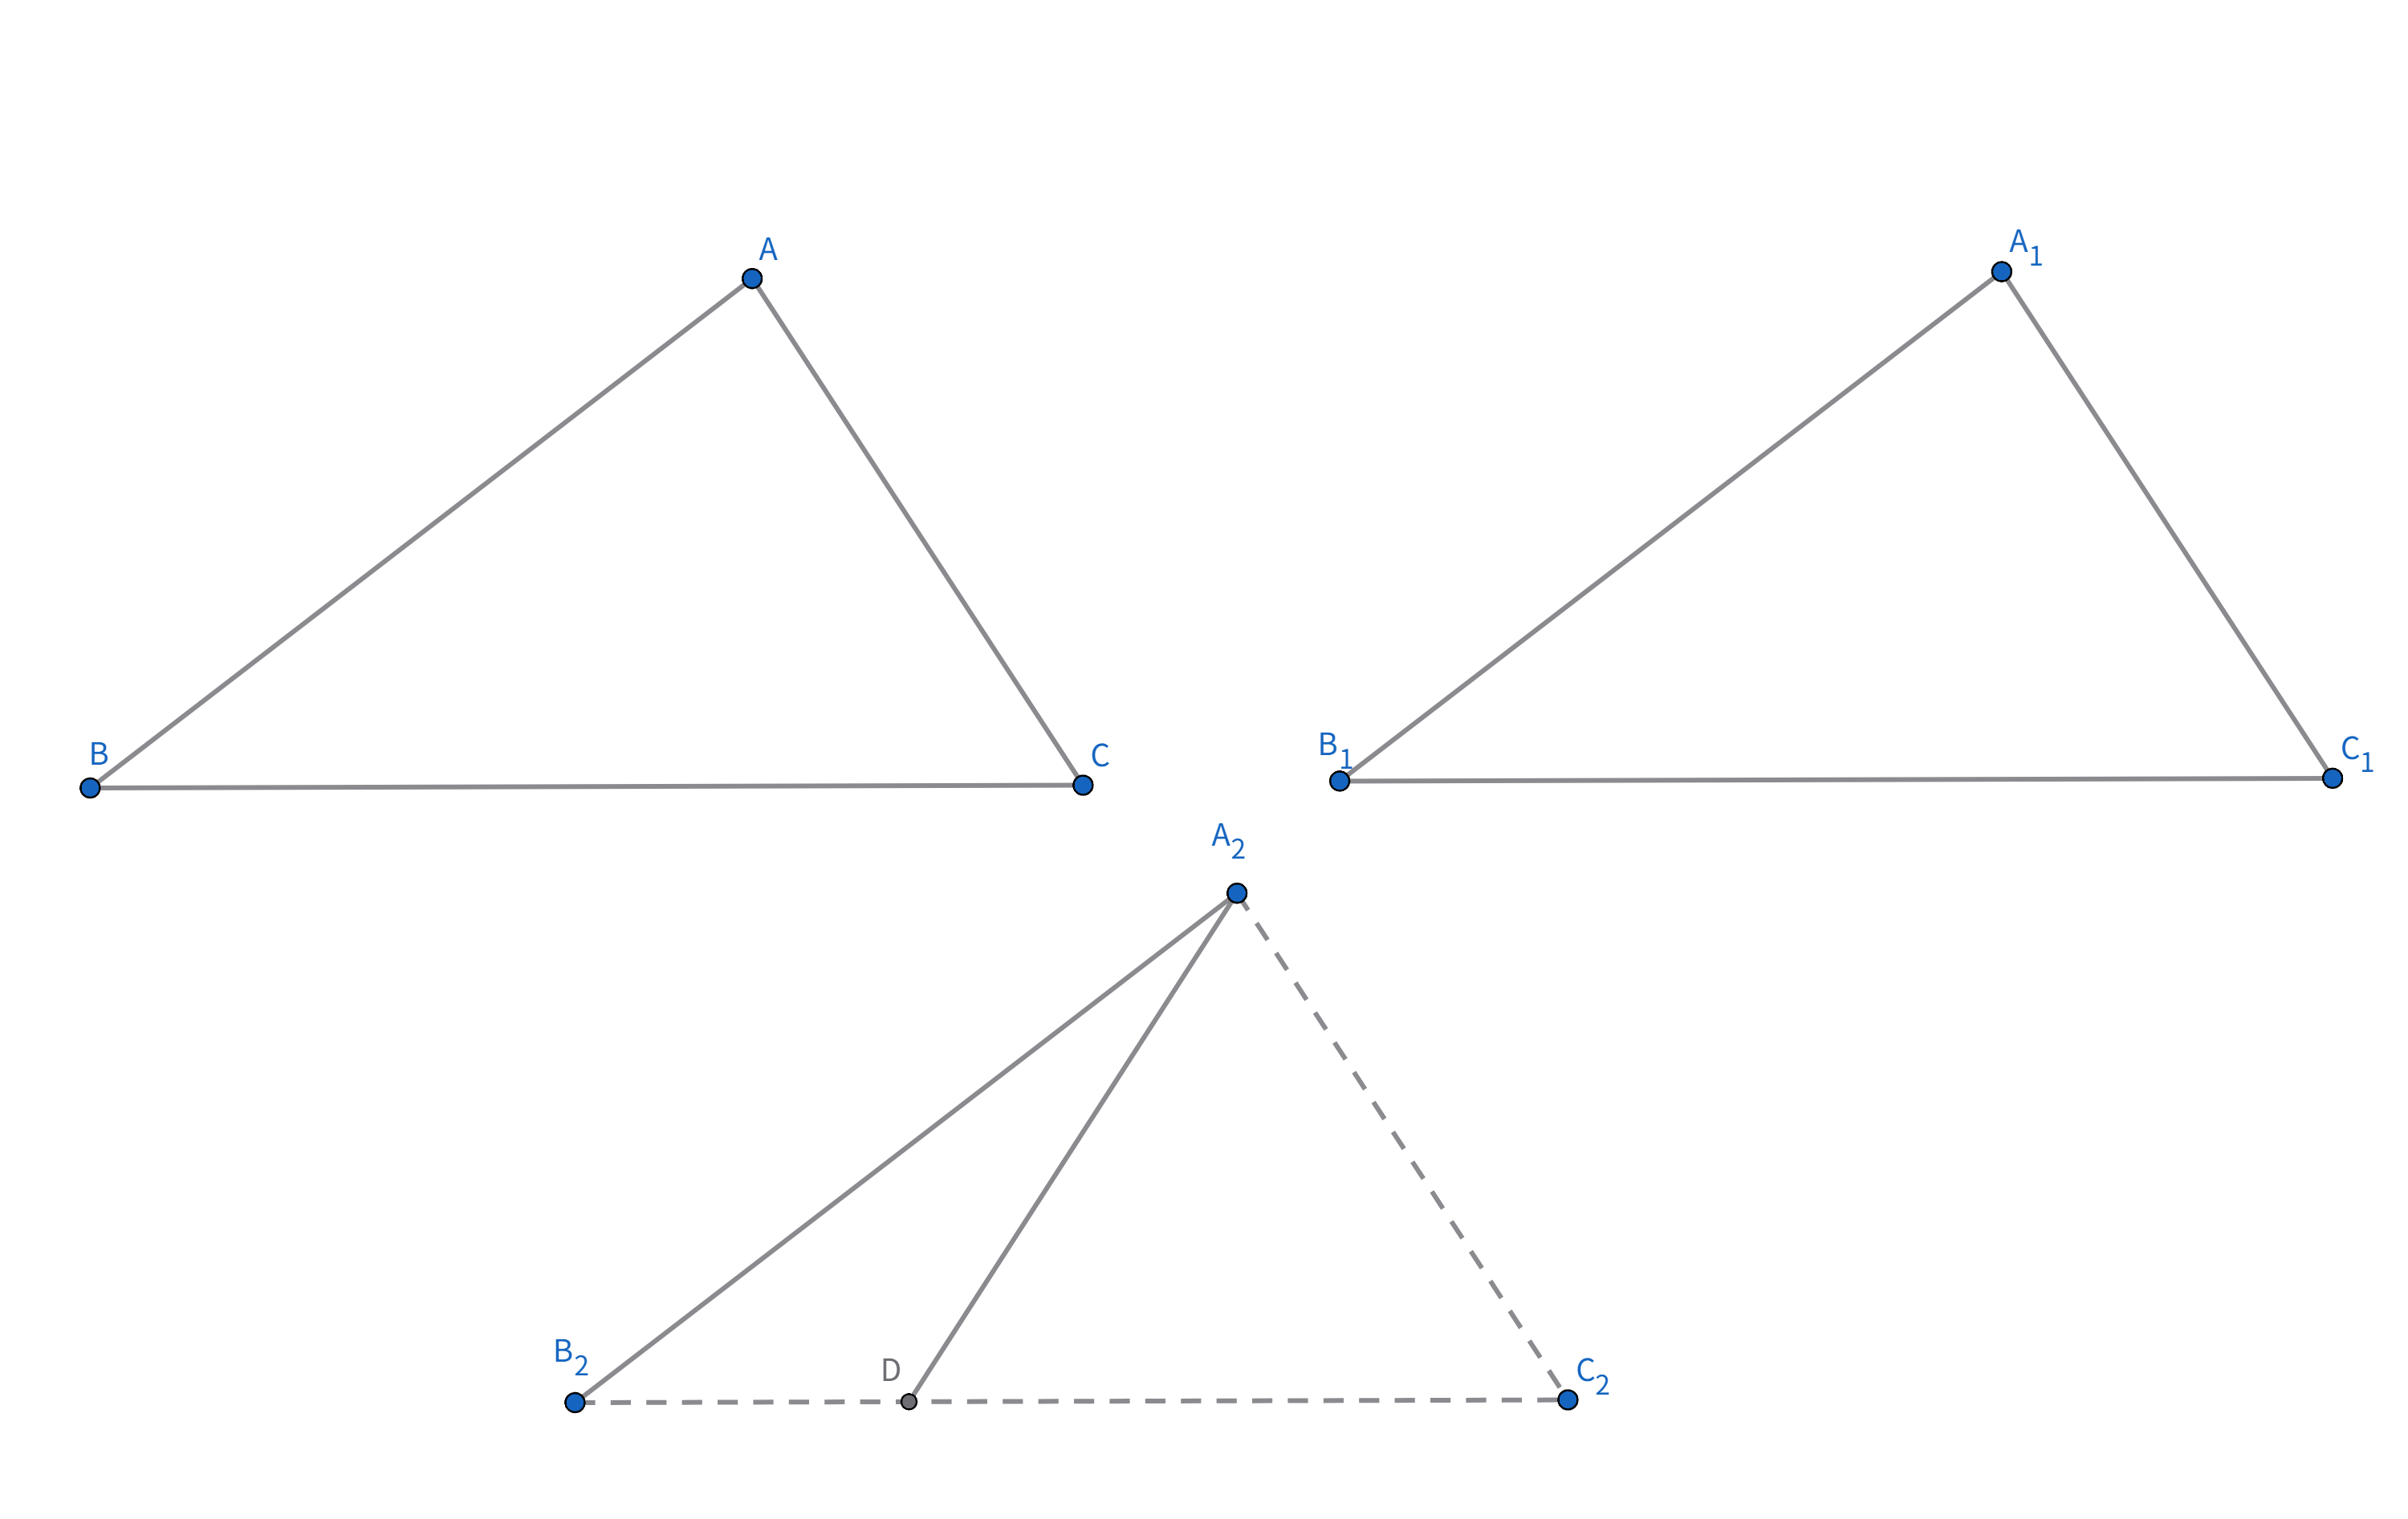
\includegraphics[width=\linewidth]{figures/全等三角形.png}
    \caption{边边角不能判定全等}
    % \label{fig:enter-label}
\end{figure}


\subsection{判定定理}
\begin{theorem}[全等三角形判定定理]
    若两三角形满足下列判别法中的其一,则一定全等。
    
    SSS (边边边): 三组边对应相等。

    SAS (边角边): 两边及其夹角对应相等。

    ASA (角边角): 两角及其夹边对应相等。

    AAS (角角边): 两角及其中一角的对边对应相等。
\end{theorem}

 
\section{平行线分线段成比例定理}
\begin{theorem}[平行线分线段成比例定理]
    假设有三条直线$l_1,l_2,l_3$互相平行,设另两条直线分别与$l_1,l_2,l_3$相交于$A,B,C$和$D,E,F$点。则
    $$\frac{AB}{BC} = \frac{DE}{EF},\quad 
    \frac{AB}{AC} = \frac{DE}{DF}, \quad 
    \frac{BC}{AC} = \frac{EF}{DF}$$
\end{theorem}
\begin{figure}[h]
    \centering
    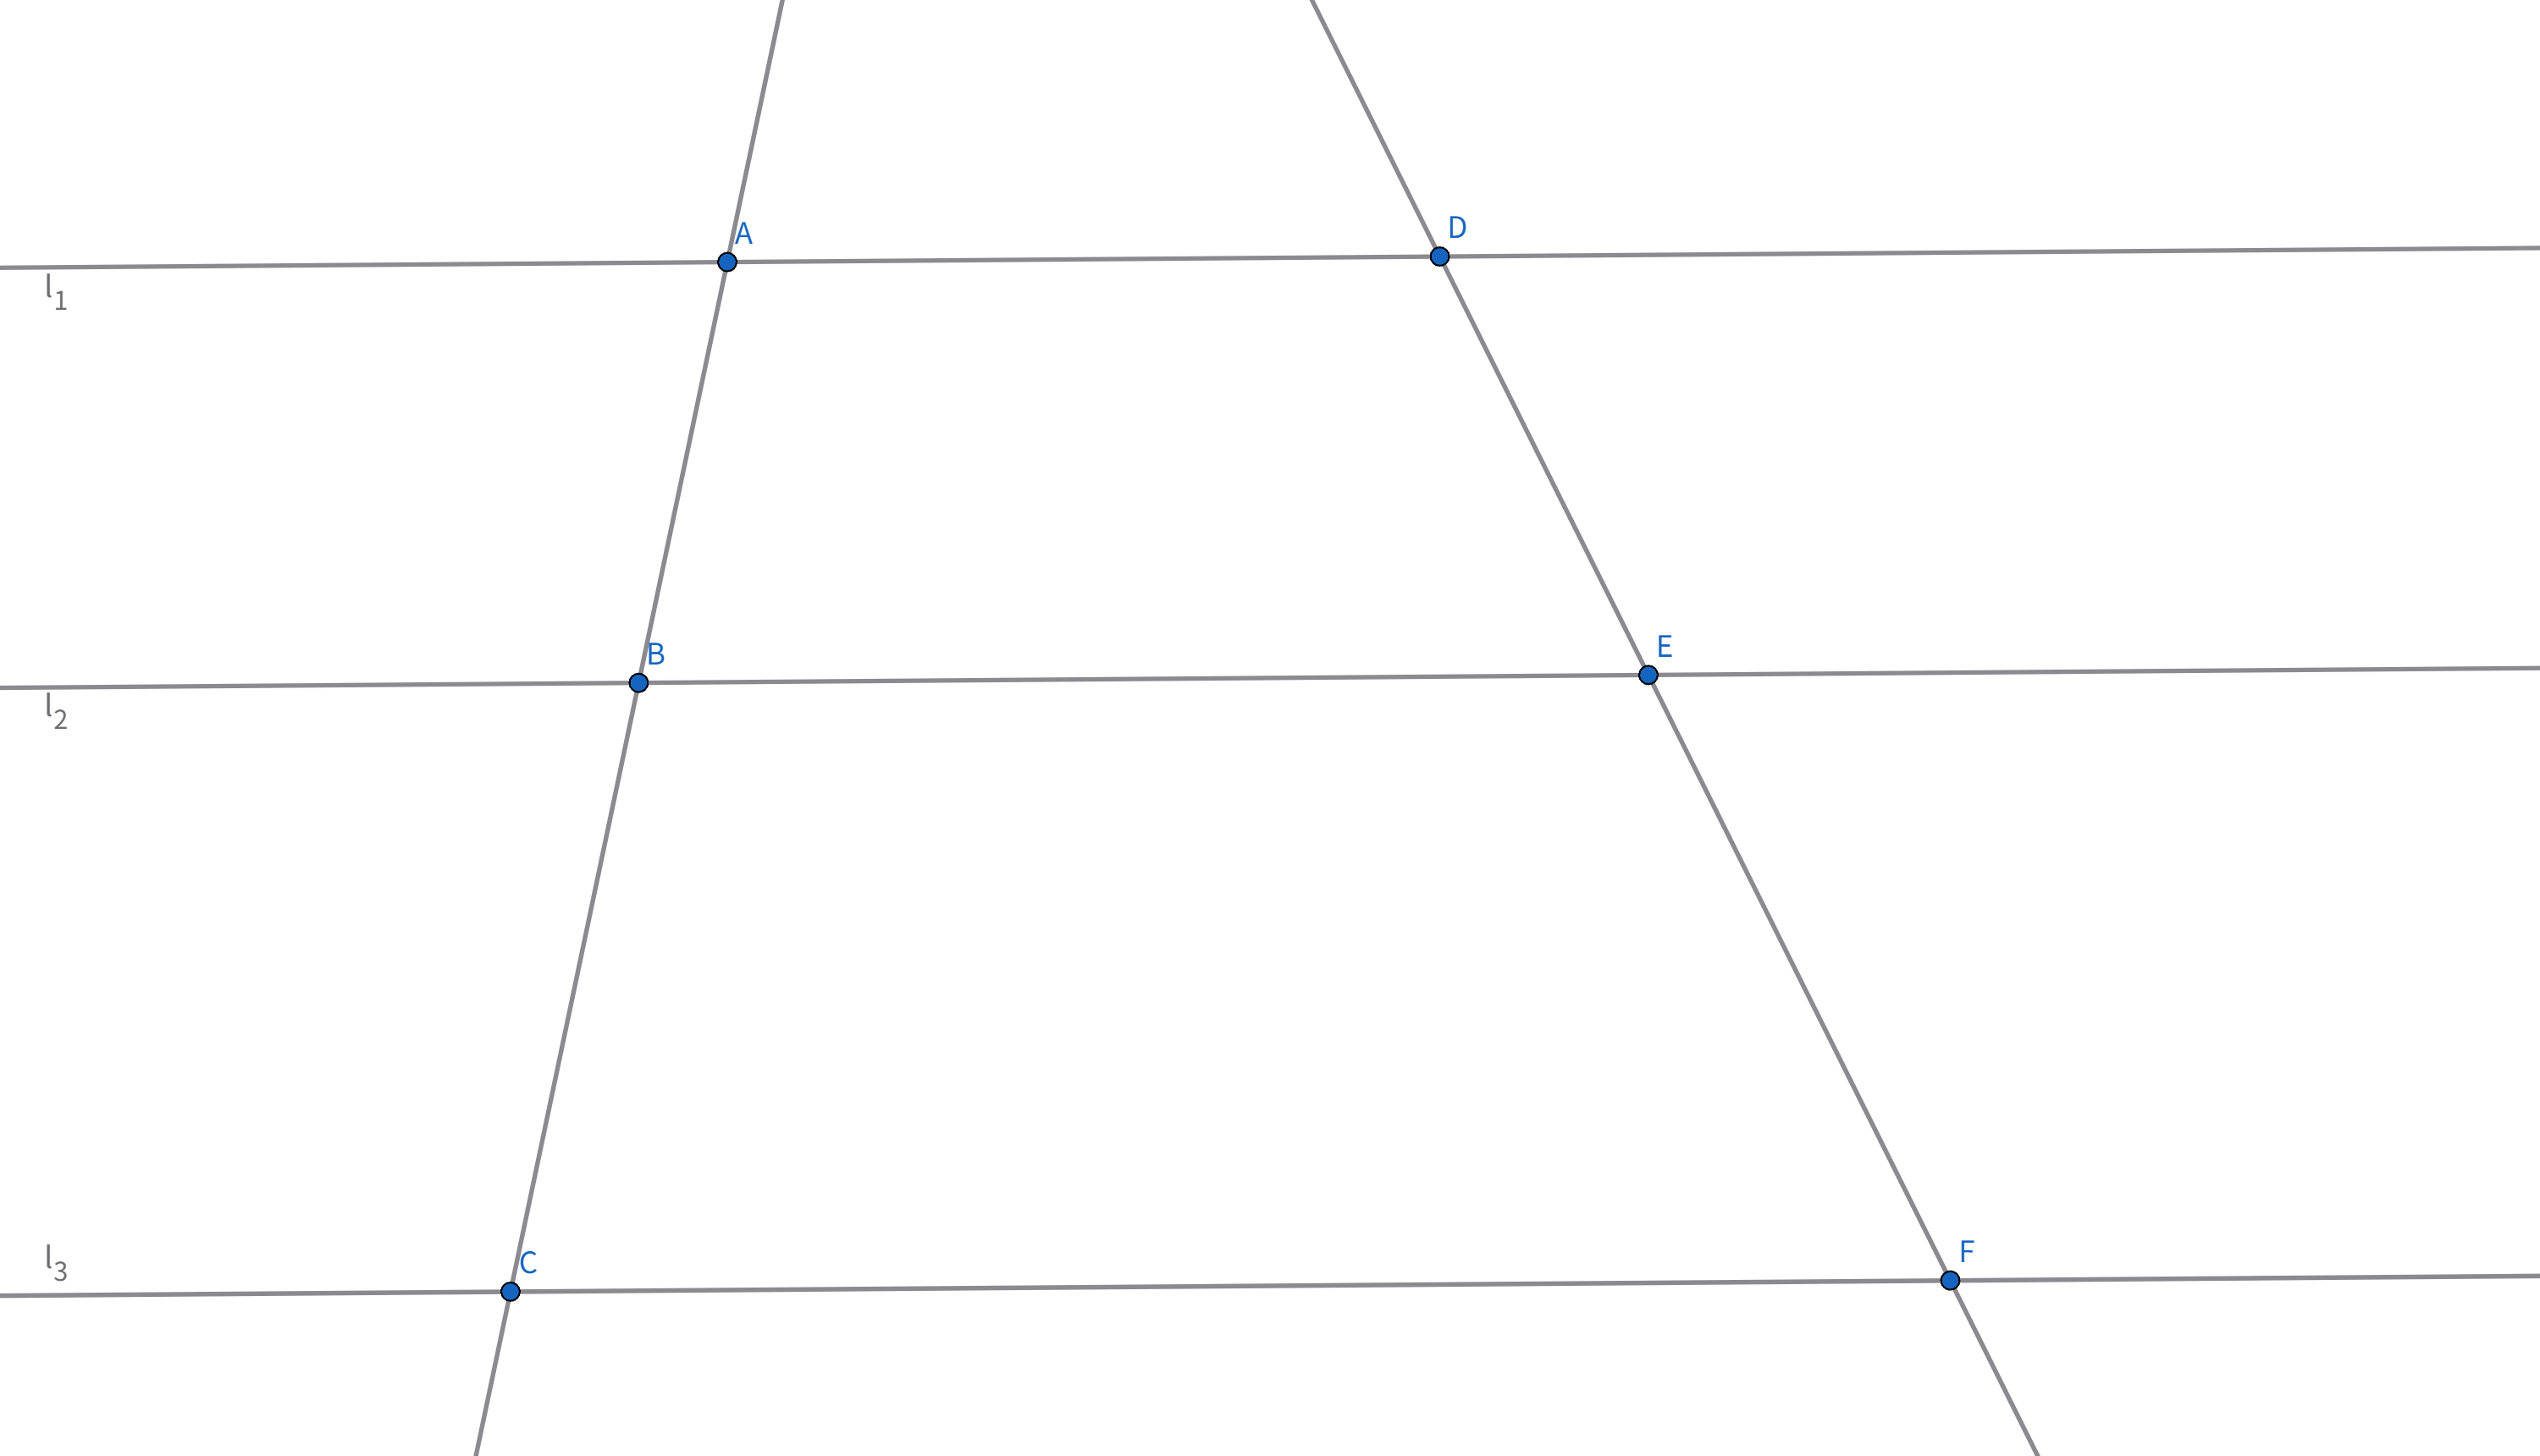
\includegraphics[width=0.8\linewidth]{figures/平行线分线段成比例.png}
    \caption{平行线分线段成比例}
    % \label{fig:enter-label}
\end{figure}

\begin{proposition}[平行相似]
    在$\triangle ABC$中,取AB、AC上的点DE平行于BC,则一定有$\triangle ABC \sim \triangle ADE$.
\end{proposition}

\begin{figure}[h]
    \centering
    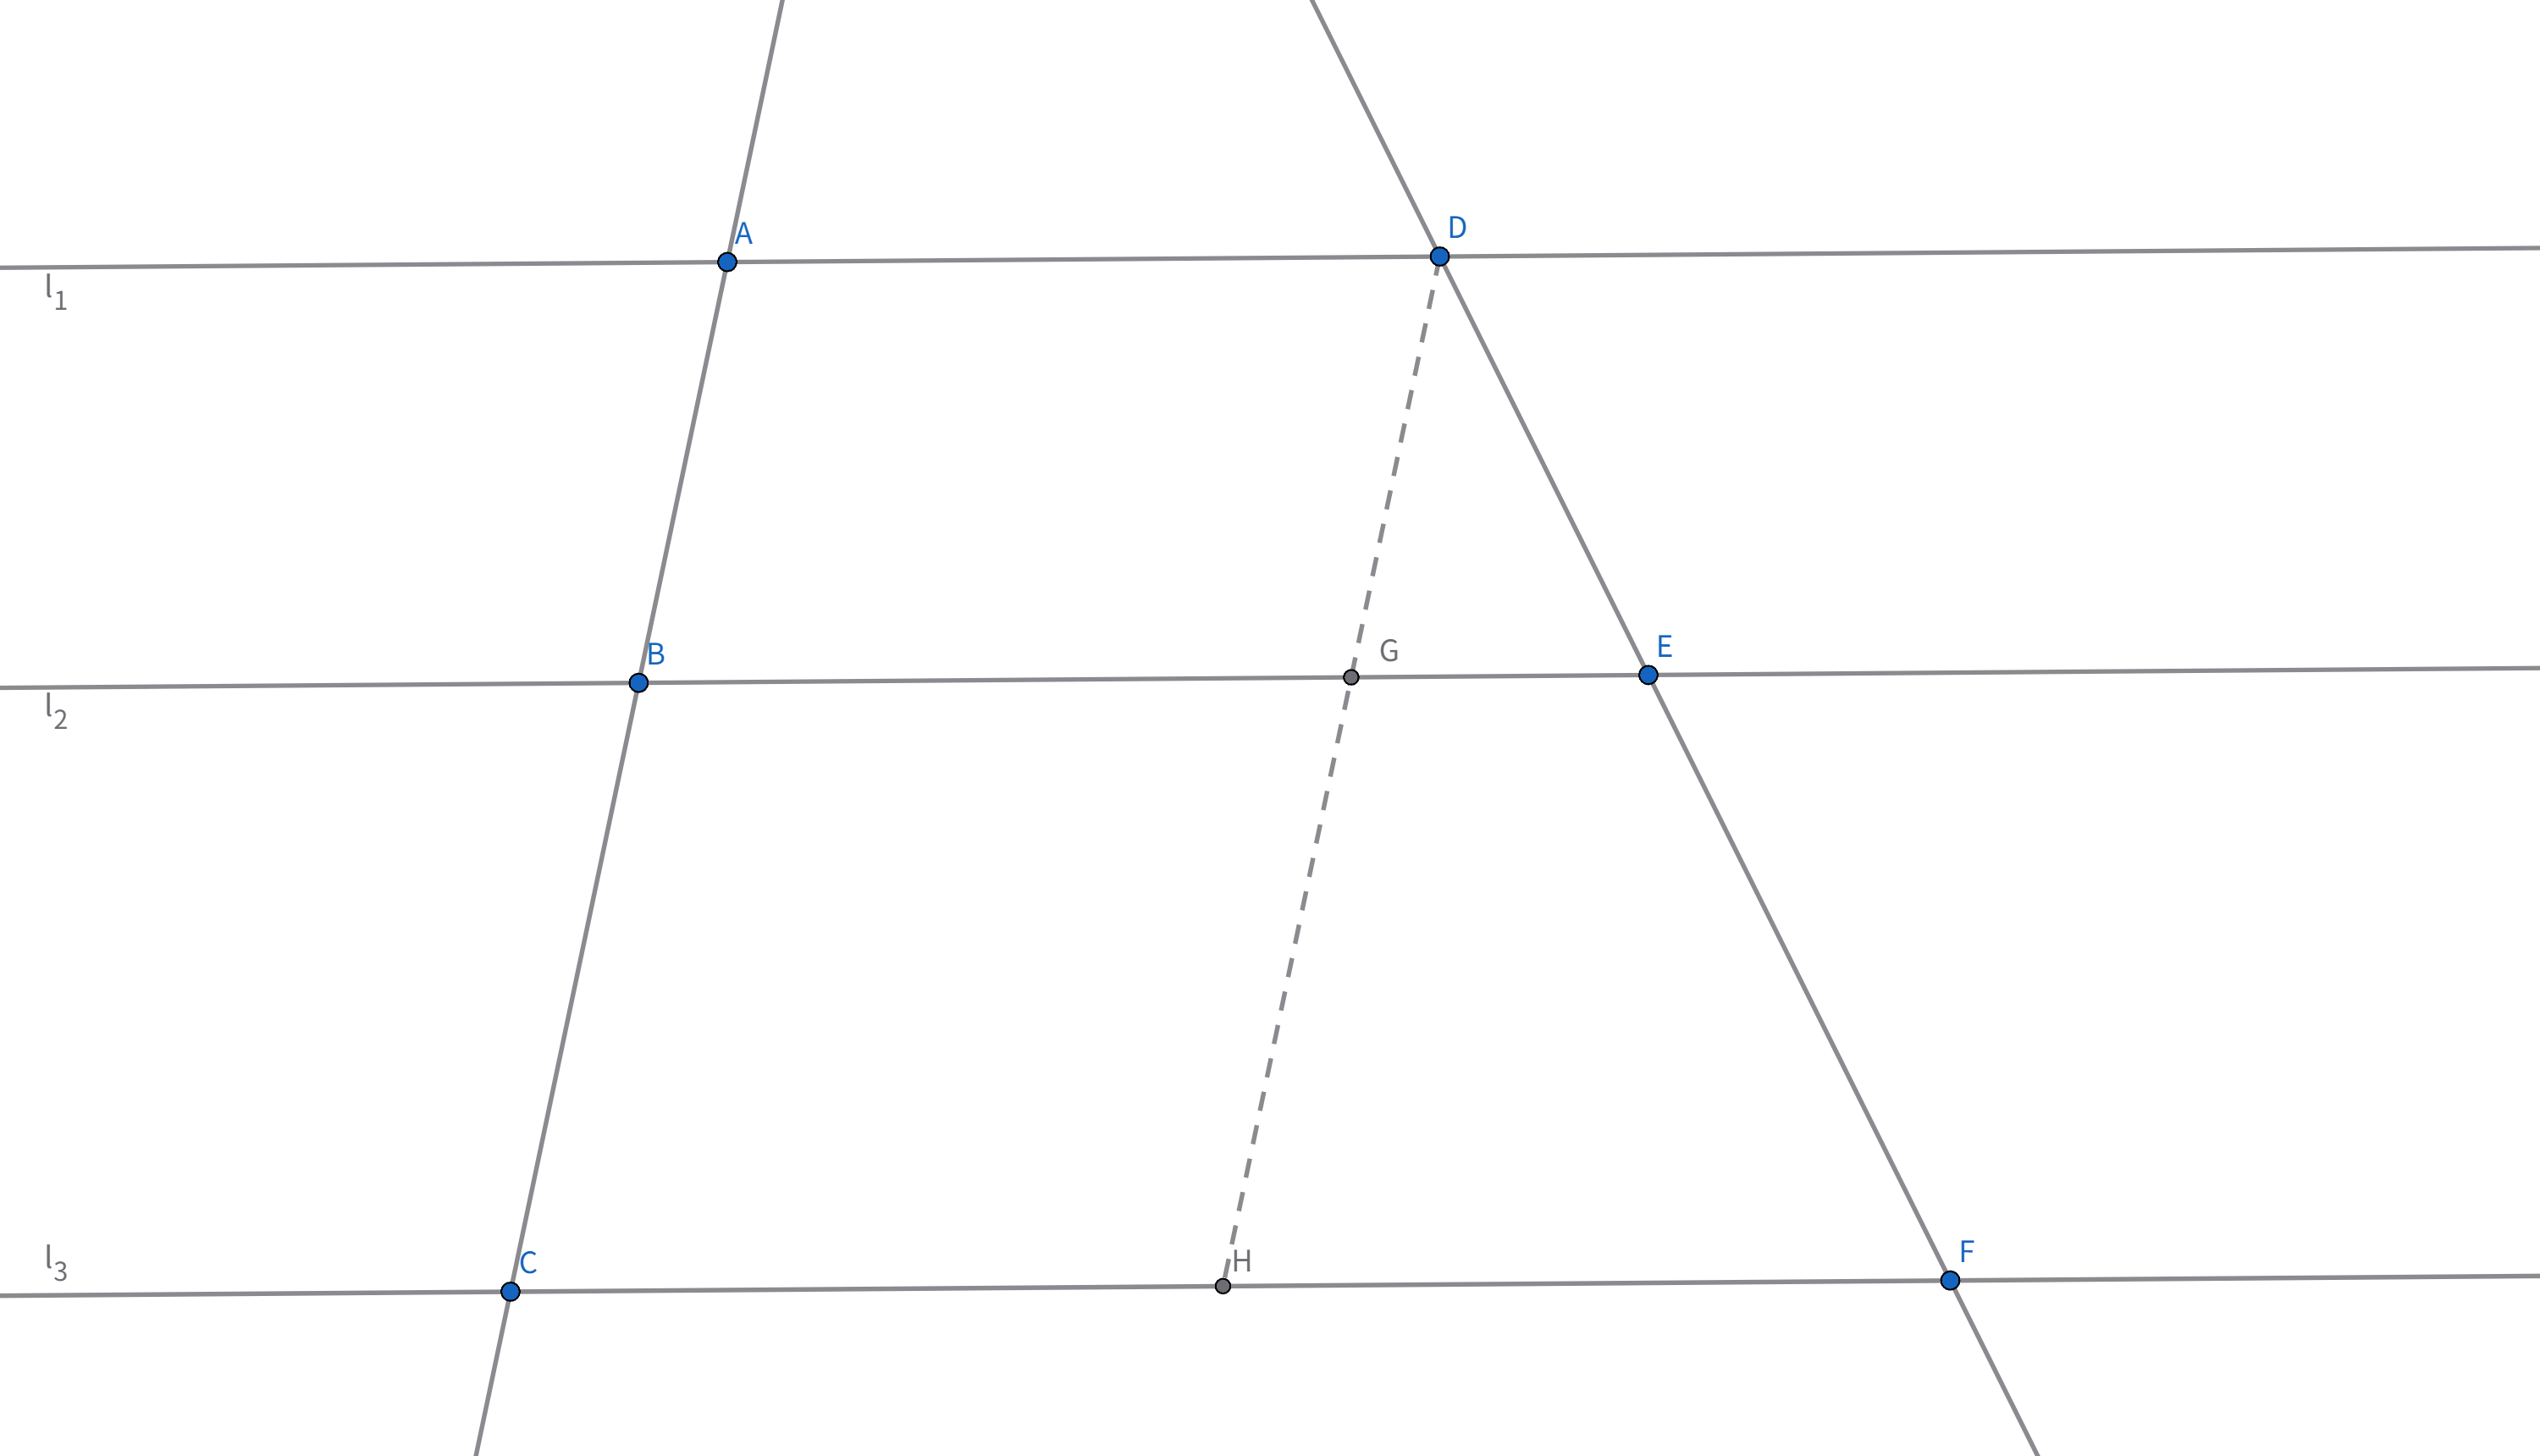
\includegraphics[width=0.8\linewidth]{figures/平行线分线段成比例 (1).png}
    \caption{平行相似}
    % \label{fig:enter-label}
\end{figure}


\section{相似三角形}
\subsection{基本概念}
\begin{definition}[相似关系]
(1) 对应角相等,对应边成比例的两个三角形叫做相似三角形。

(2) 若$\triangle ABC$与$\triangle DEF$相似,记作
    $$\triangle ABC \sim \triangle DEF.$$
(3) 相似三角形的三组对应角全部相等,即
    $$\angle A = \angle D, \quad \angle B = \angle E, \quad \angle C = \angle F.$$
(4) 相似三角形的三组对应边比例相等,即
    $$\frac{AB}{DE} = \frac{BC}{EF} = \frac{AC}{DF}=k.$$
    $k$称作是$\triangle ABC$与$\triangle DEF$的相似比。特别的,k=1时两三角形即为全等。
\end{definition}

\begin{figure}[h]
    \centering
    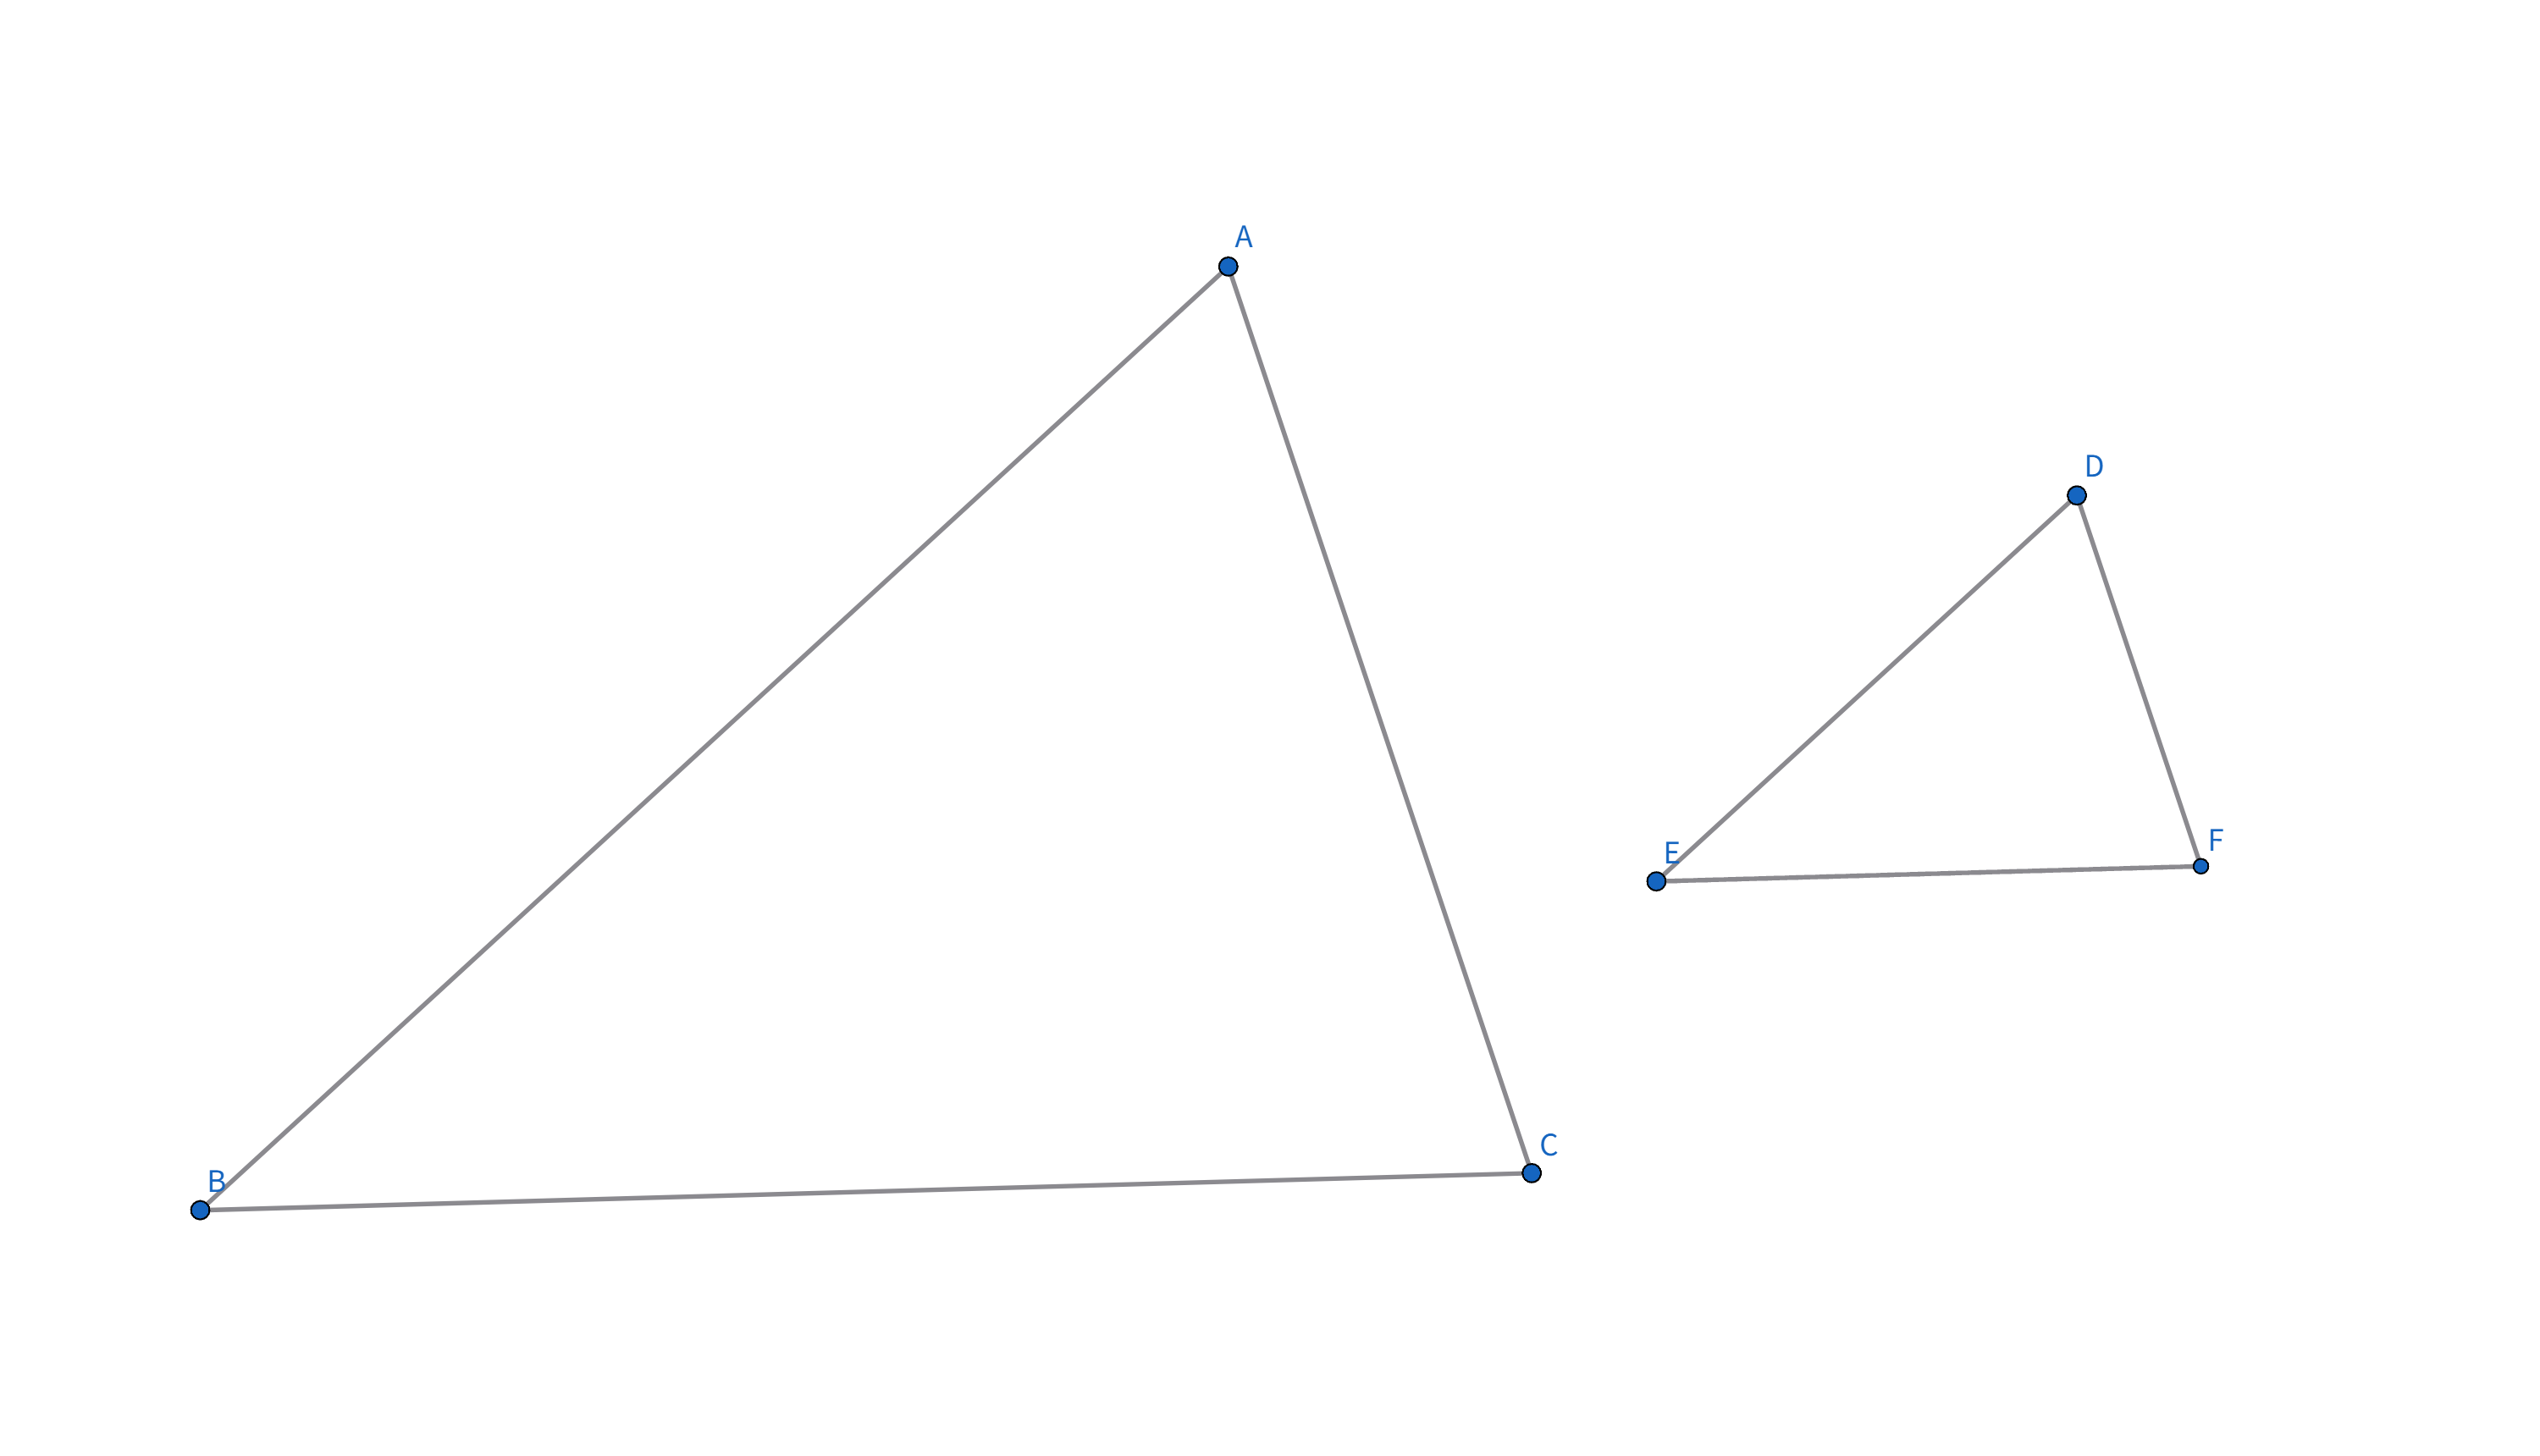
\includegraphics[width=0.8\linewidth]{figures/相似三角形.png}
    \caption{相似三角形}
    % \label{fig:enter-label}
\end{figure}
\begin{proposition}
    (5) 相似三角形的对应线段比也都等于相似比$k$,例如对应高线、角平分线、中线、中位线等。
    
    (6) 相似三角形的面积比为相似比的平方,即
    $$\frac{S_{\triangle ABC}}{S_{\triangle DEF}} = k^2.$$
    
    (6) 相似三角形同样具有传递性。
\end{proposition}

\subsection{判定定理}
\begin{theorem}
    若两三角形满足下列判别法中的其一,则一定相似。

    AA (角角) / AAA (角角角): 两角对应相等,则两三角形相似。
    
    SAS (边角边): 两边对应成比例且夹角相等,则两三角形相似。

    SSS (边边边): 三边对应成比例,则两三角形相似。
\end{theorem}
\begin{figure}[h]
    \centering
    \hfill % 添加一些水平间距
    \begin{minipage}[t]{0.3\textwidth}
        \centering
        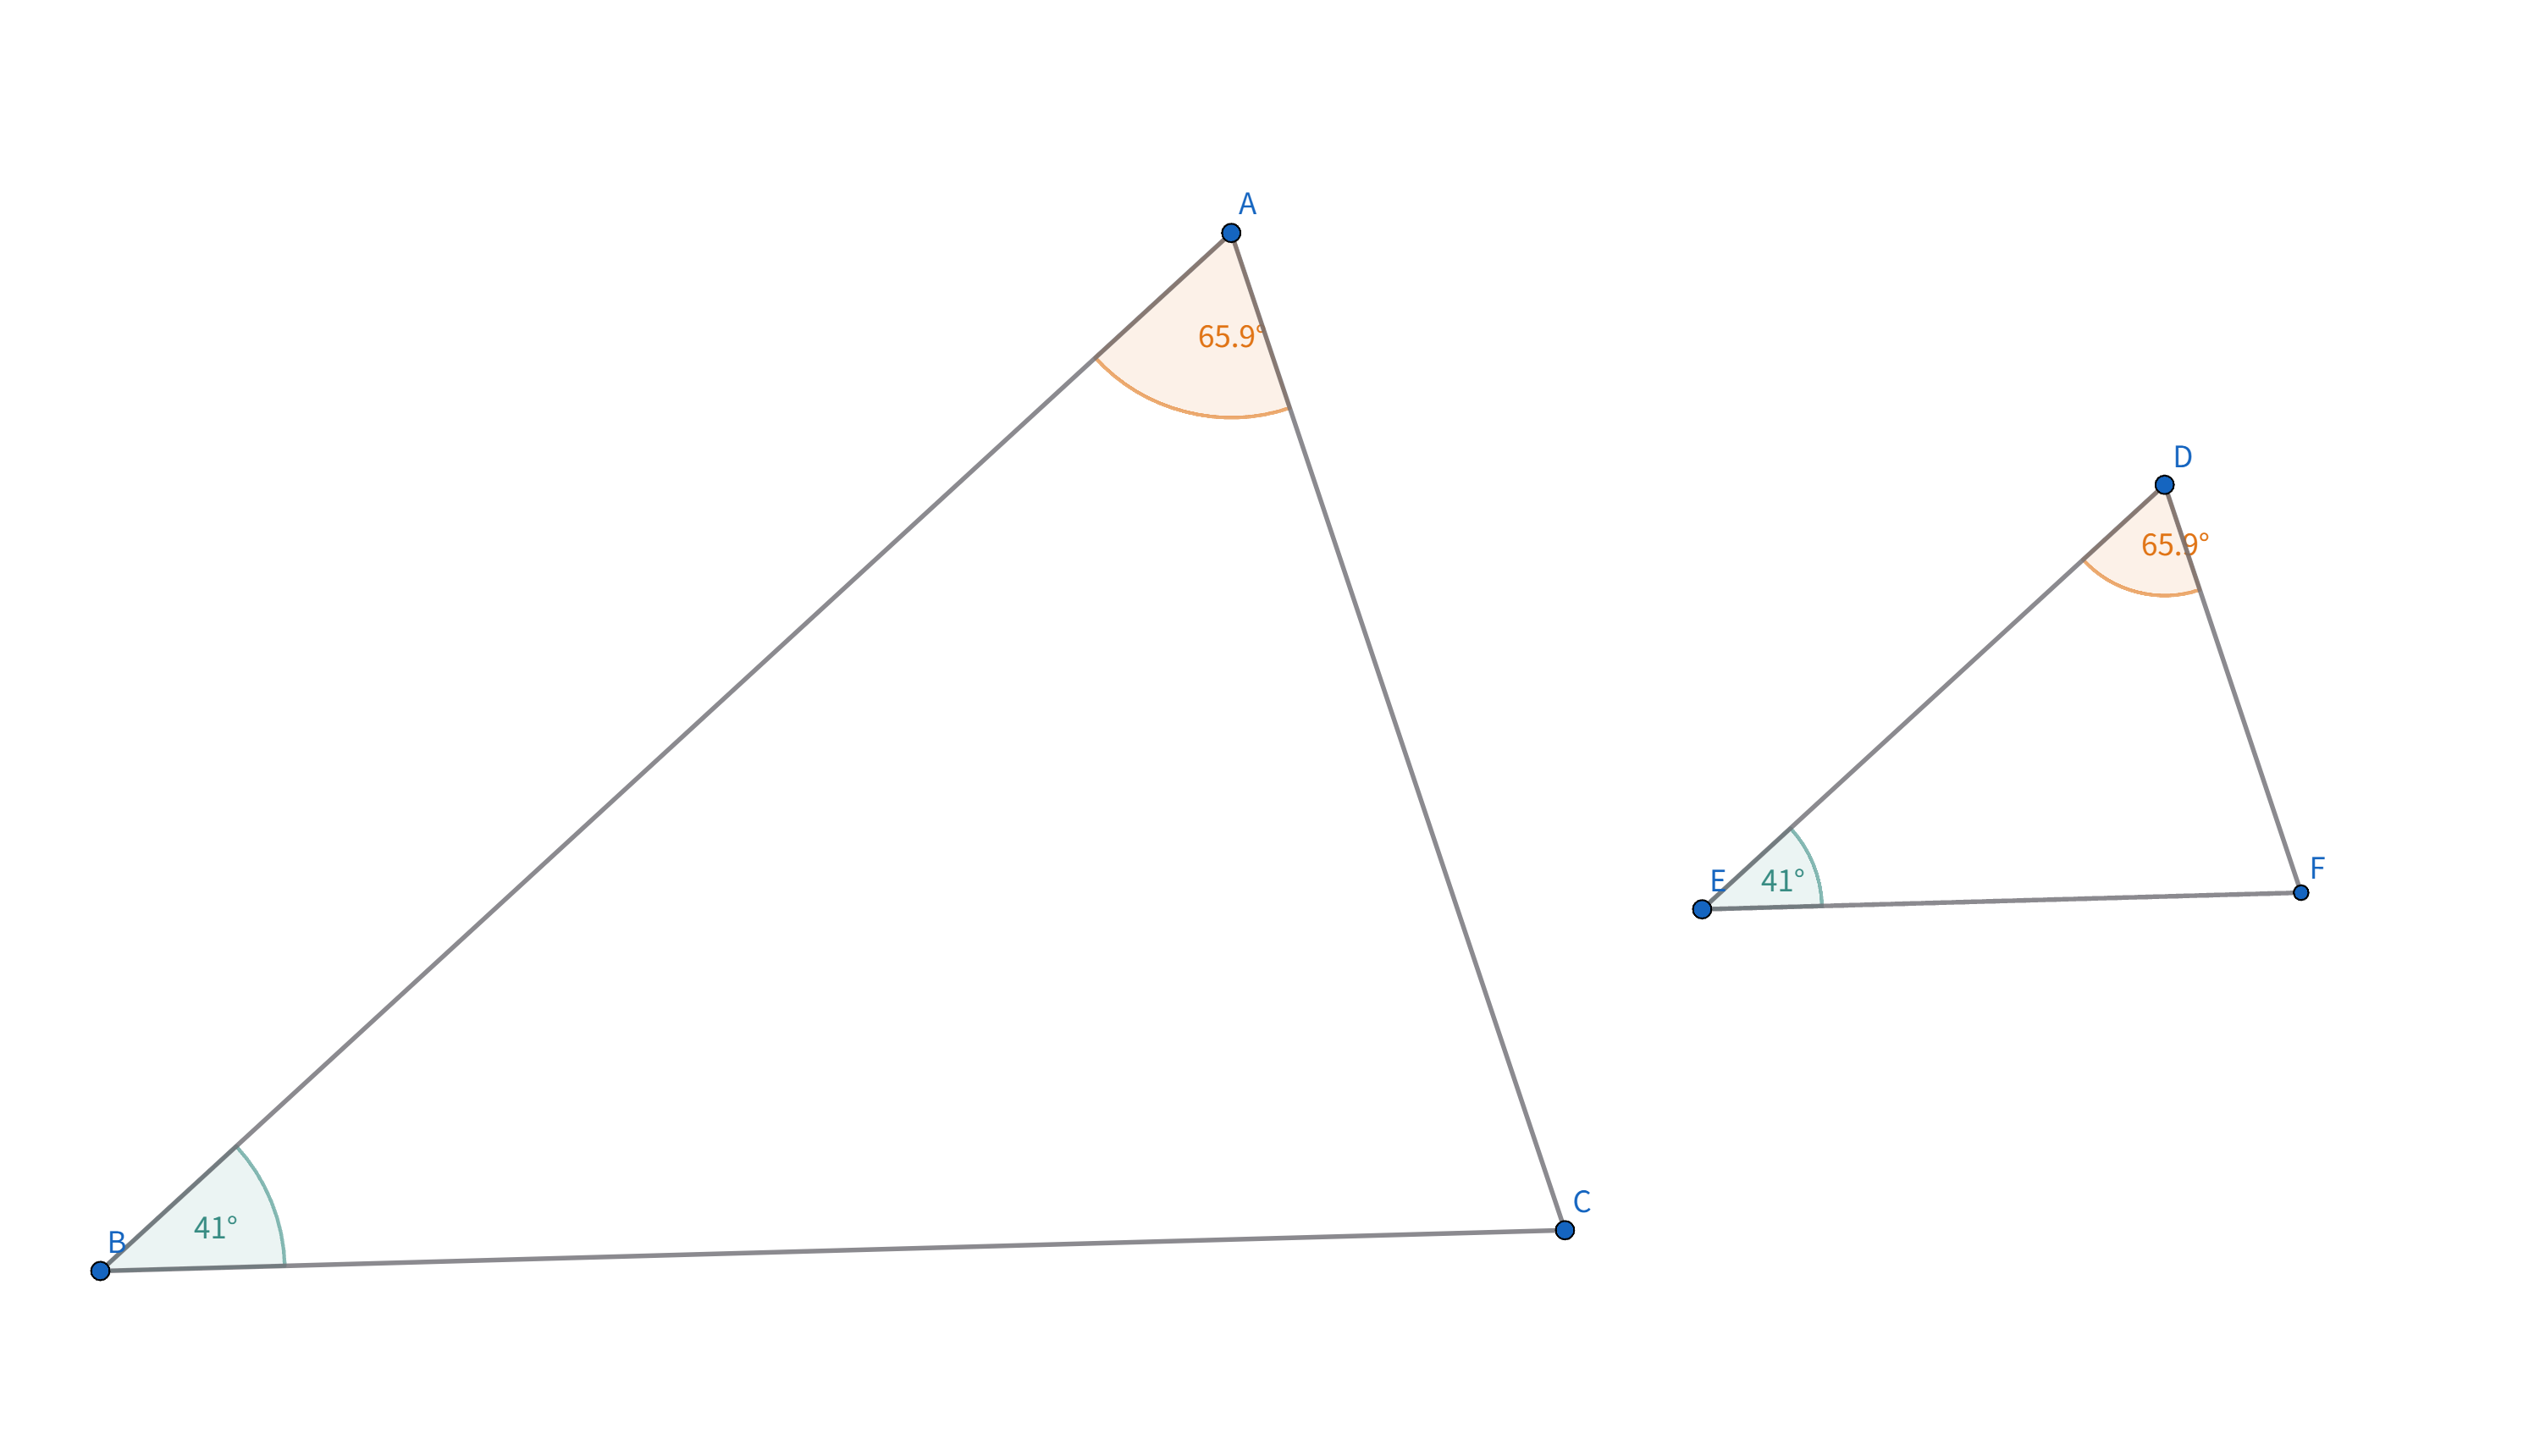
\includegraphics[width=\linewidth]{figures/AA相似.png}
        \caption{AA相似}
        % \label{fig:side:b}
    \end{minipage}
    \hfill % 添加一些水平间距
    \begin{minipage}[t]{0.3\textwidth}
    \centering
    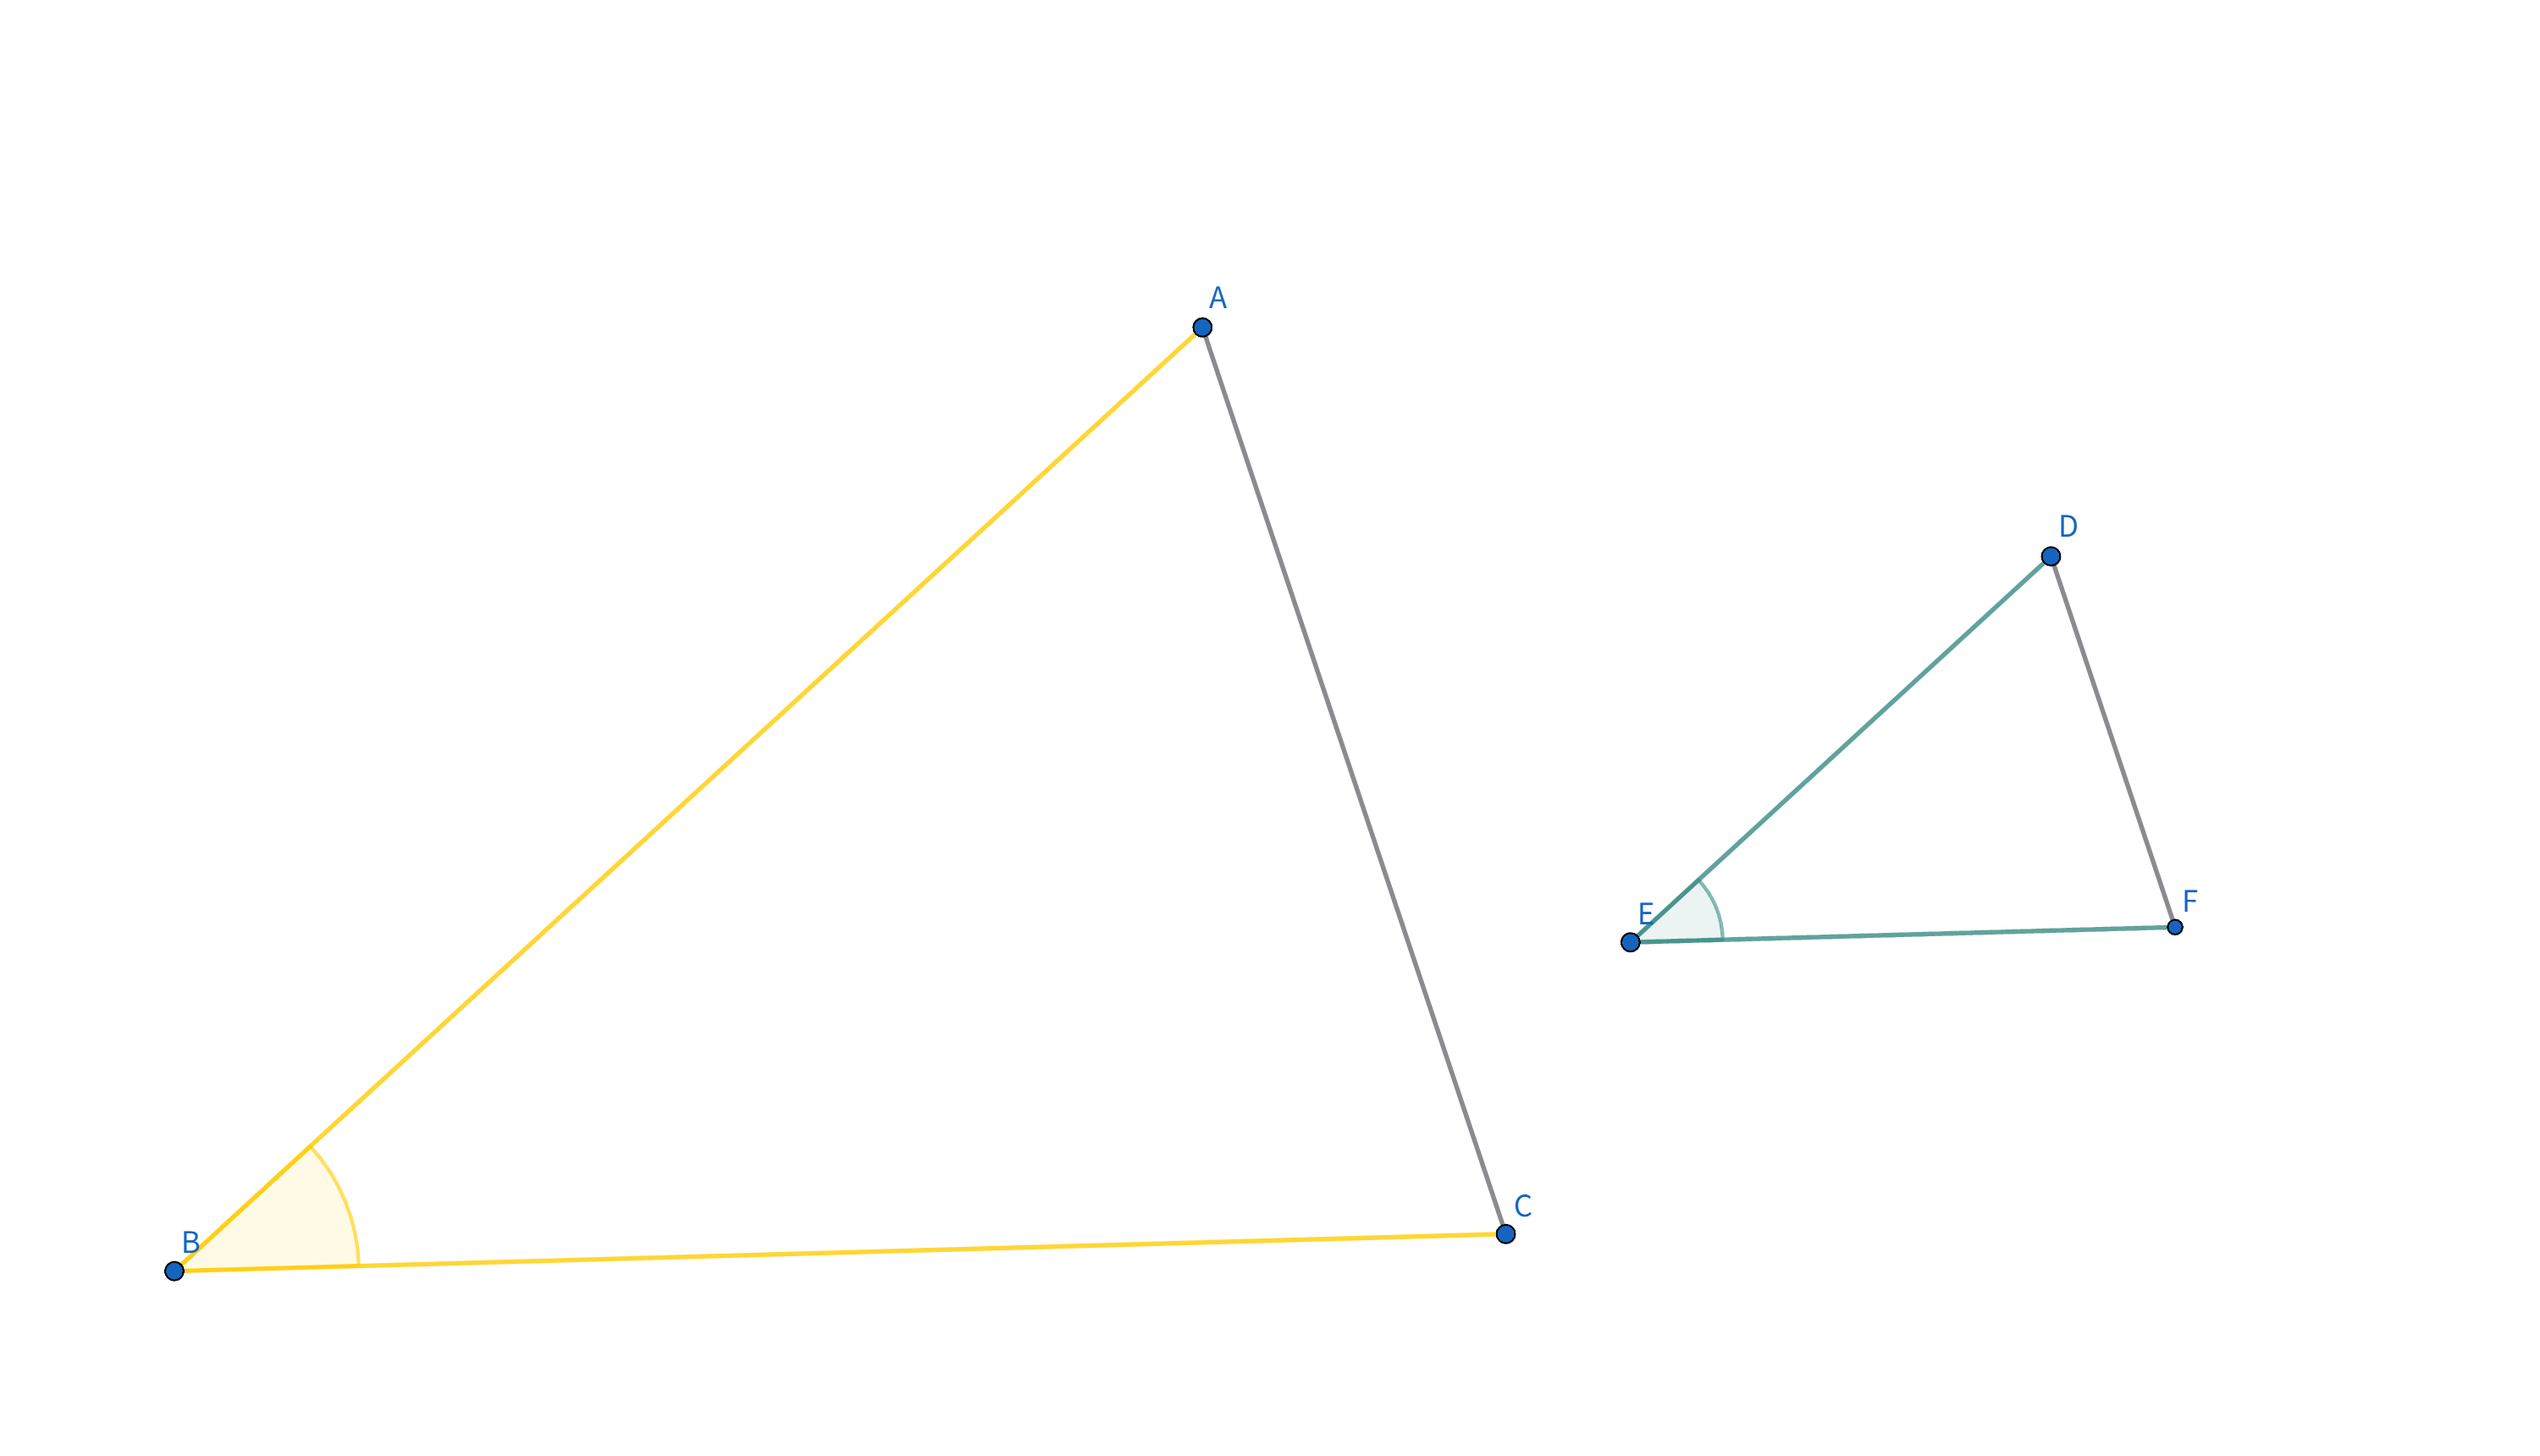
\includegraphics[width=\linewidth]{figures/SAS相似.png}
    \caption{SAS相似}
    \end{minipage}
    \begin{minipage}[t]{0.3\textwidth}
    \centering
    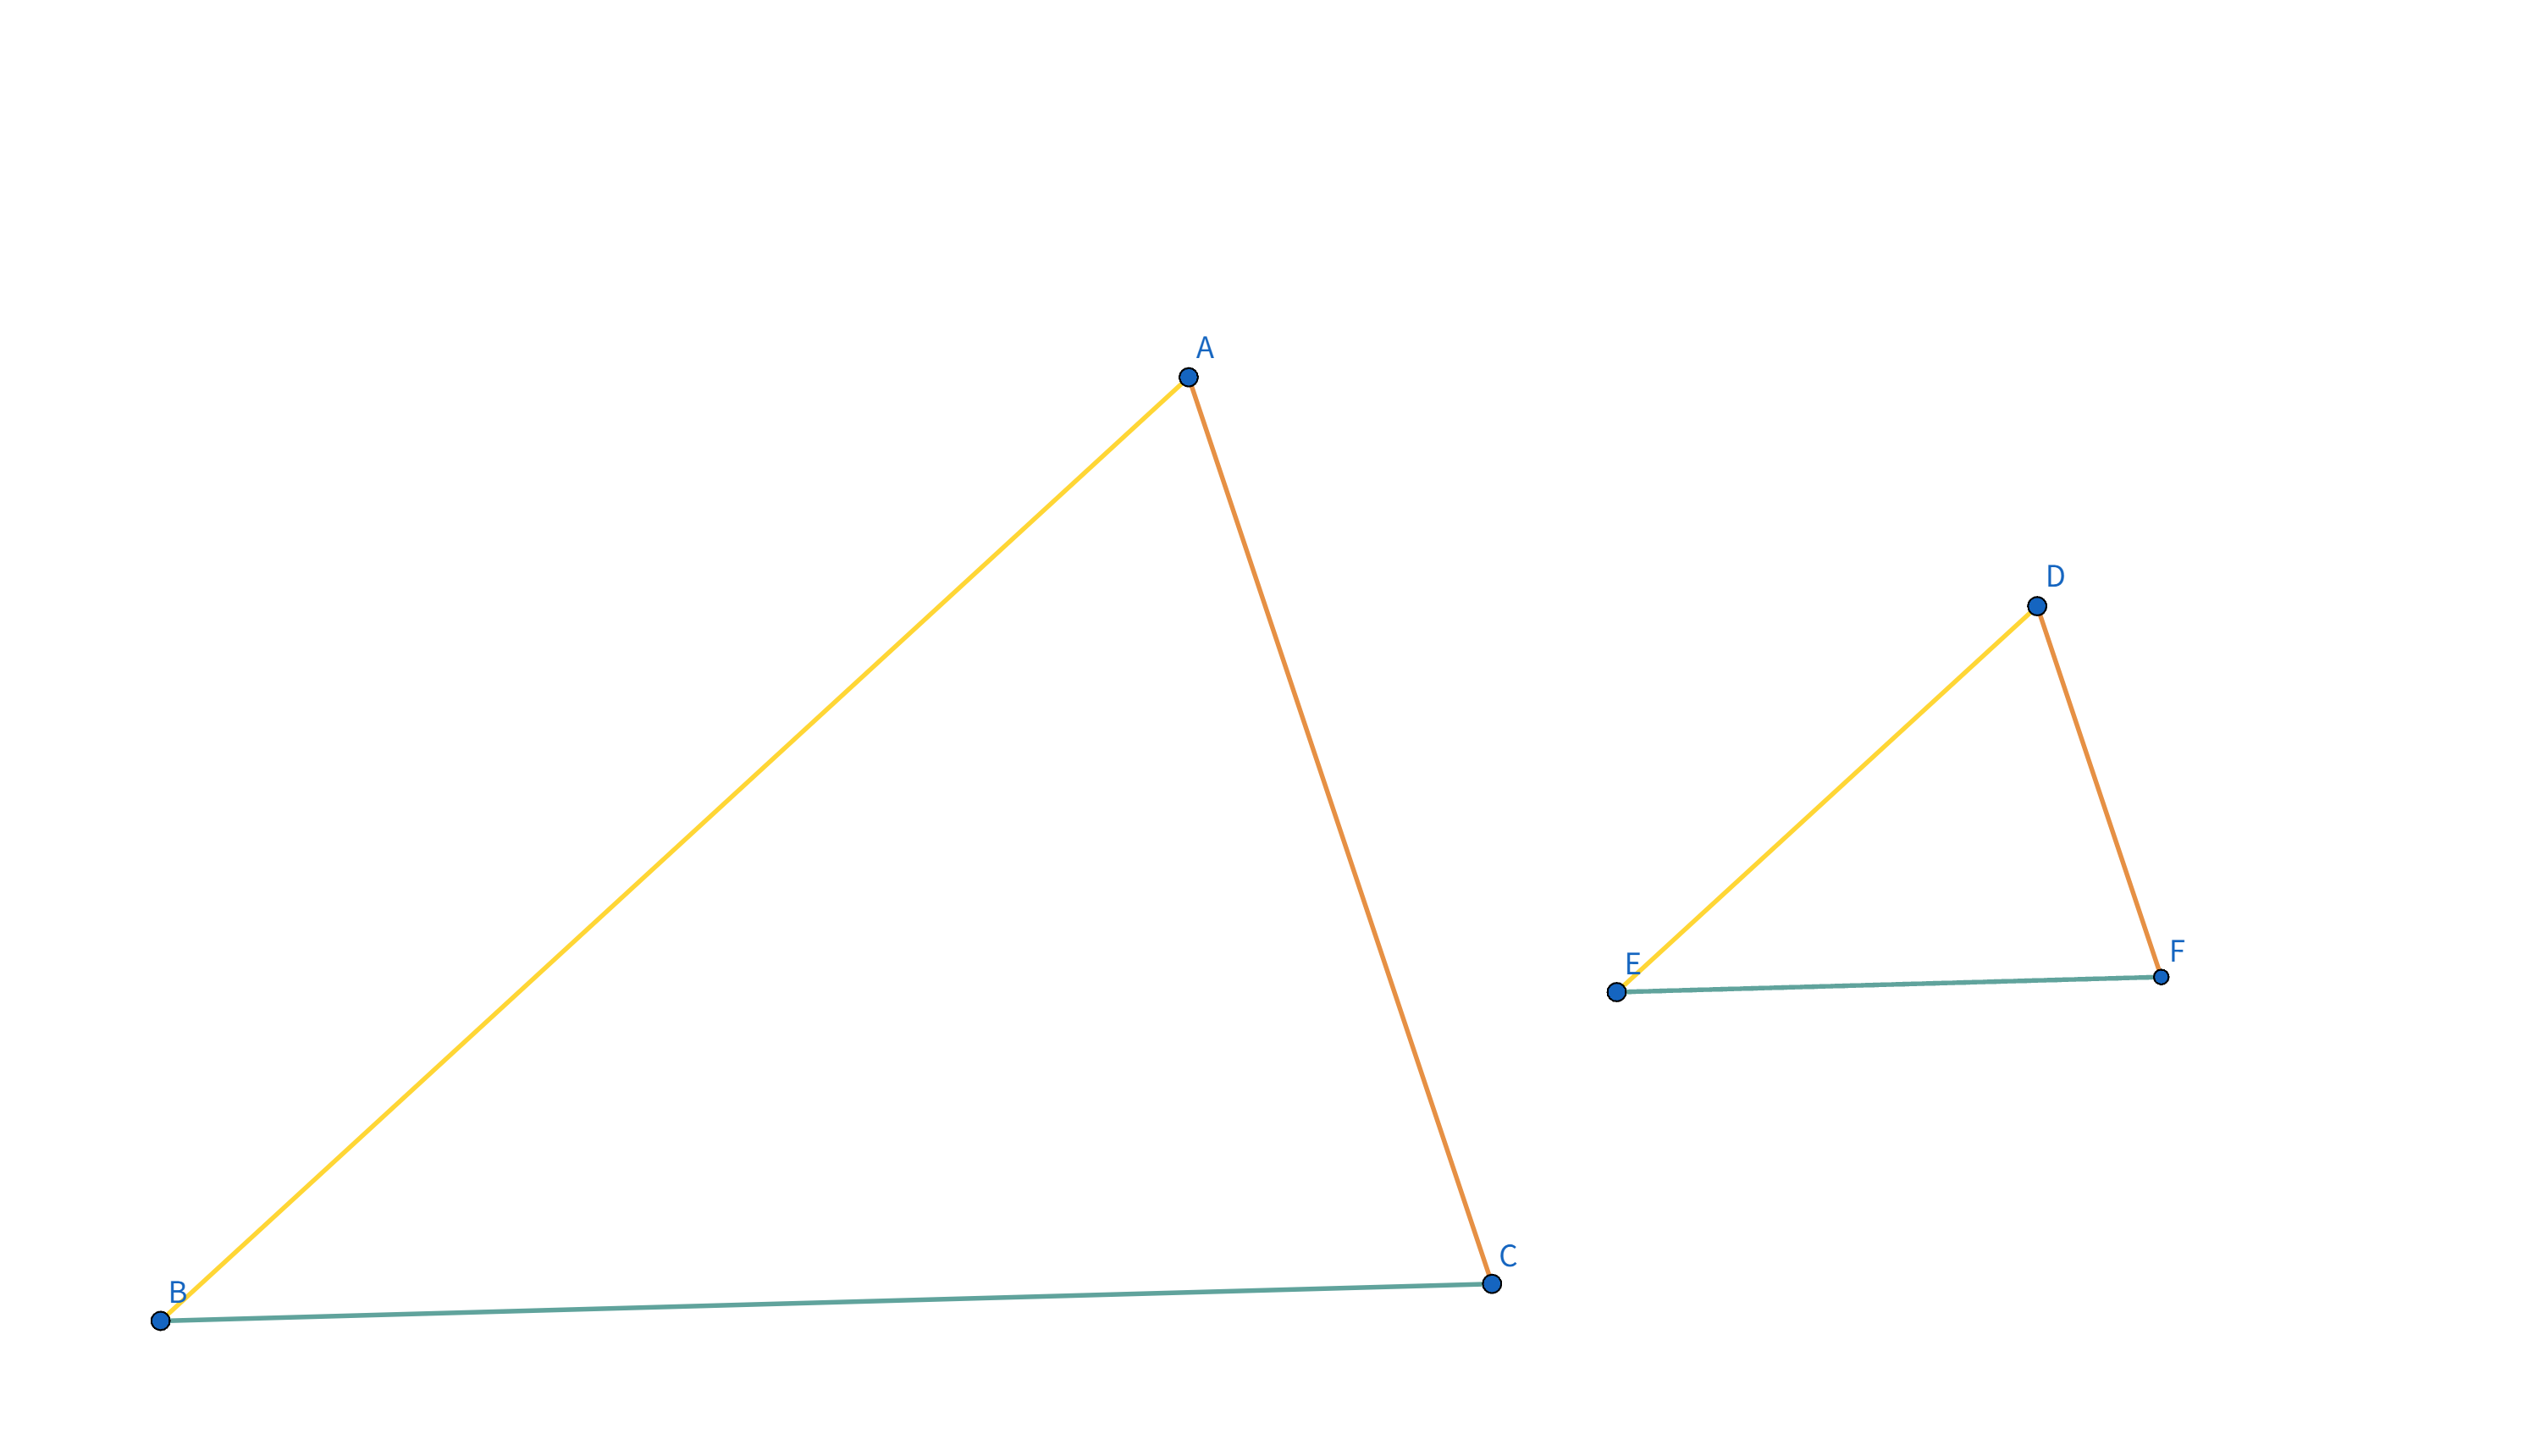
\includegraphics[width=\linewidth]{figures/SSS相似.png}
    \caption{SSS相似}
    \end{minipage}
\end{figure}












\subsection{常见形式}

\begin{figure}[h]
    \centering
    \hfill % 添加一些水平间距
    \begin{minipage}[t]{0.45\textwidth}
    \centering
    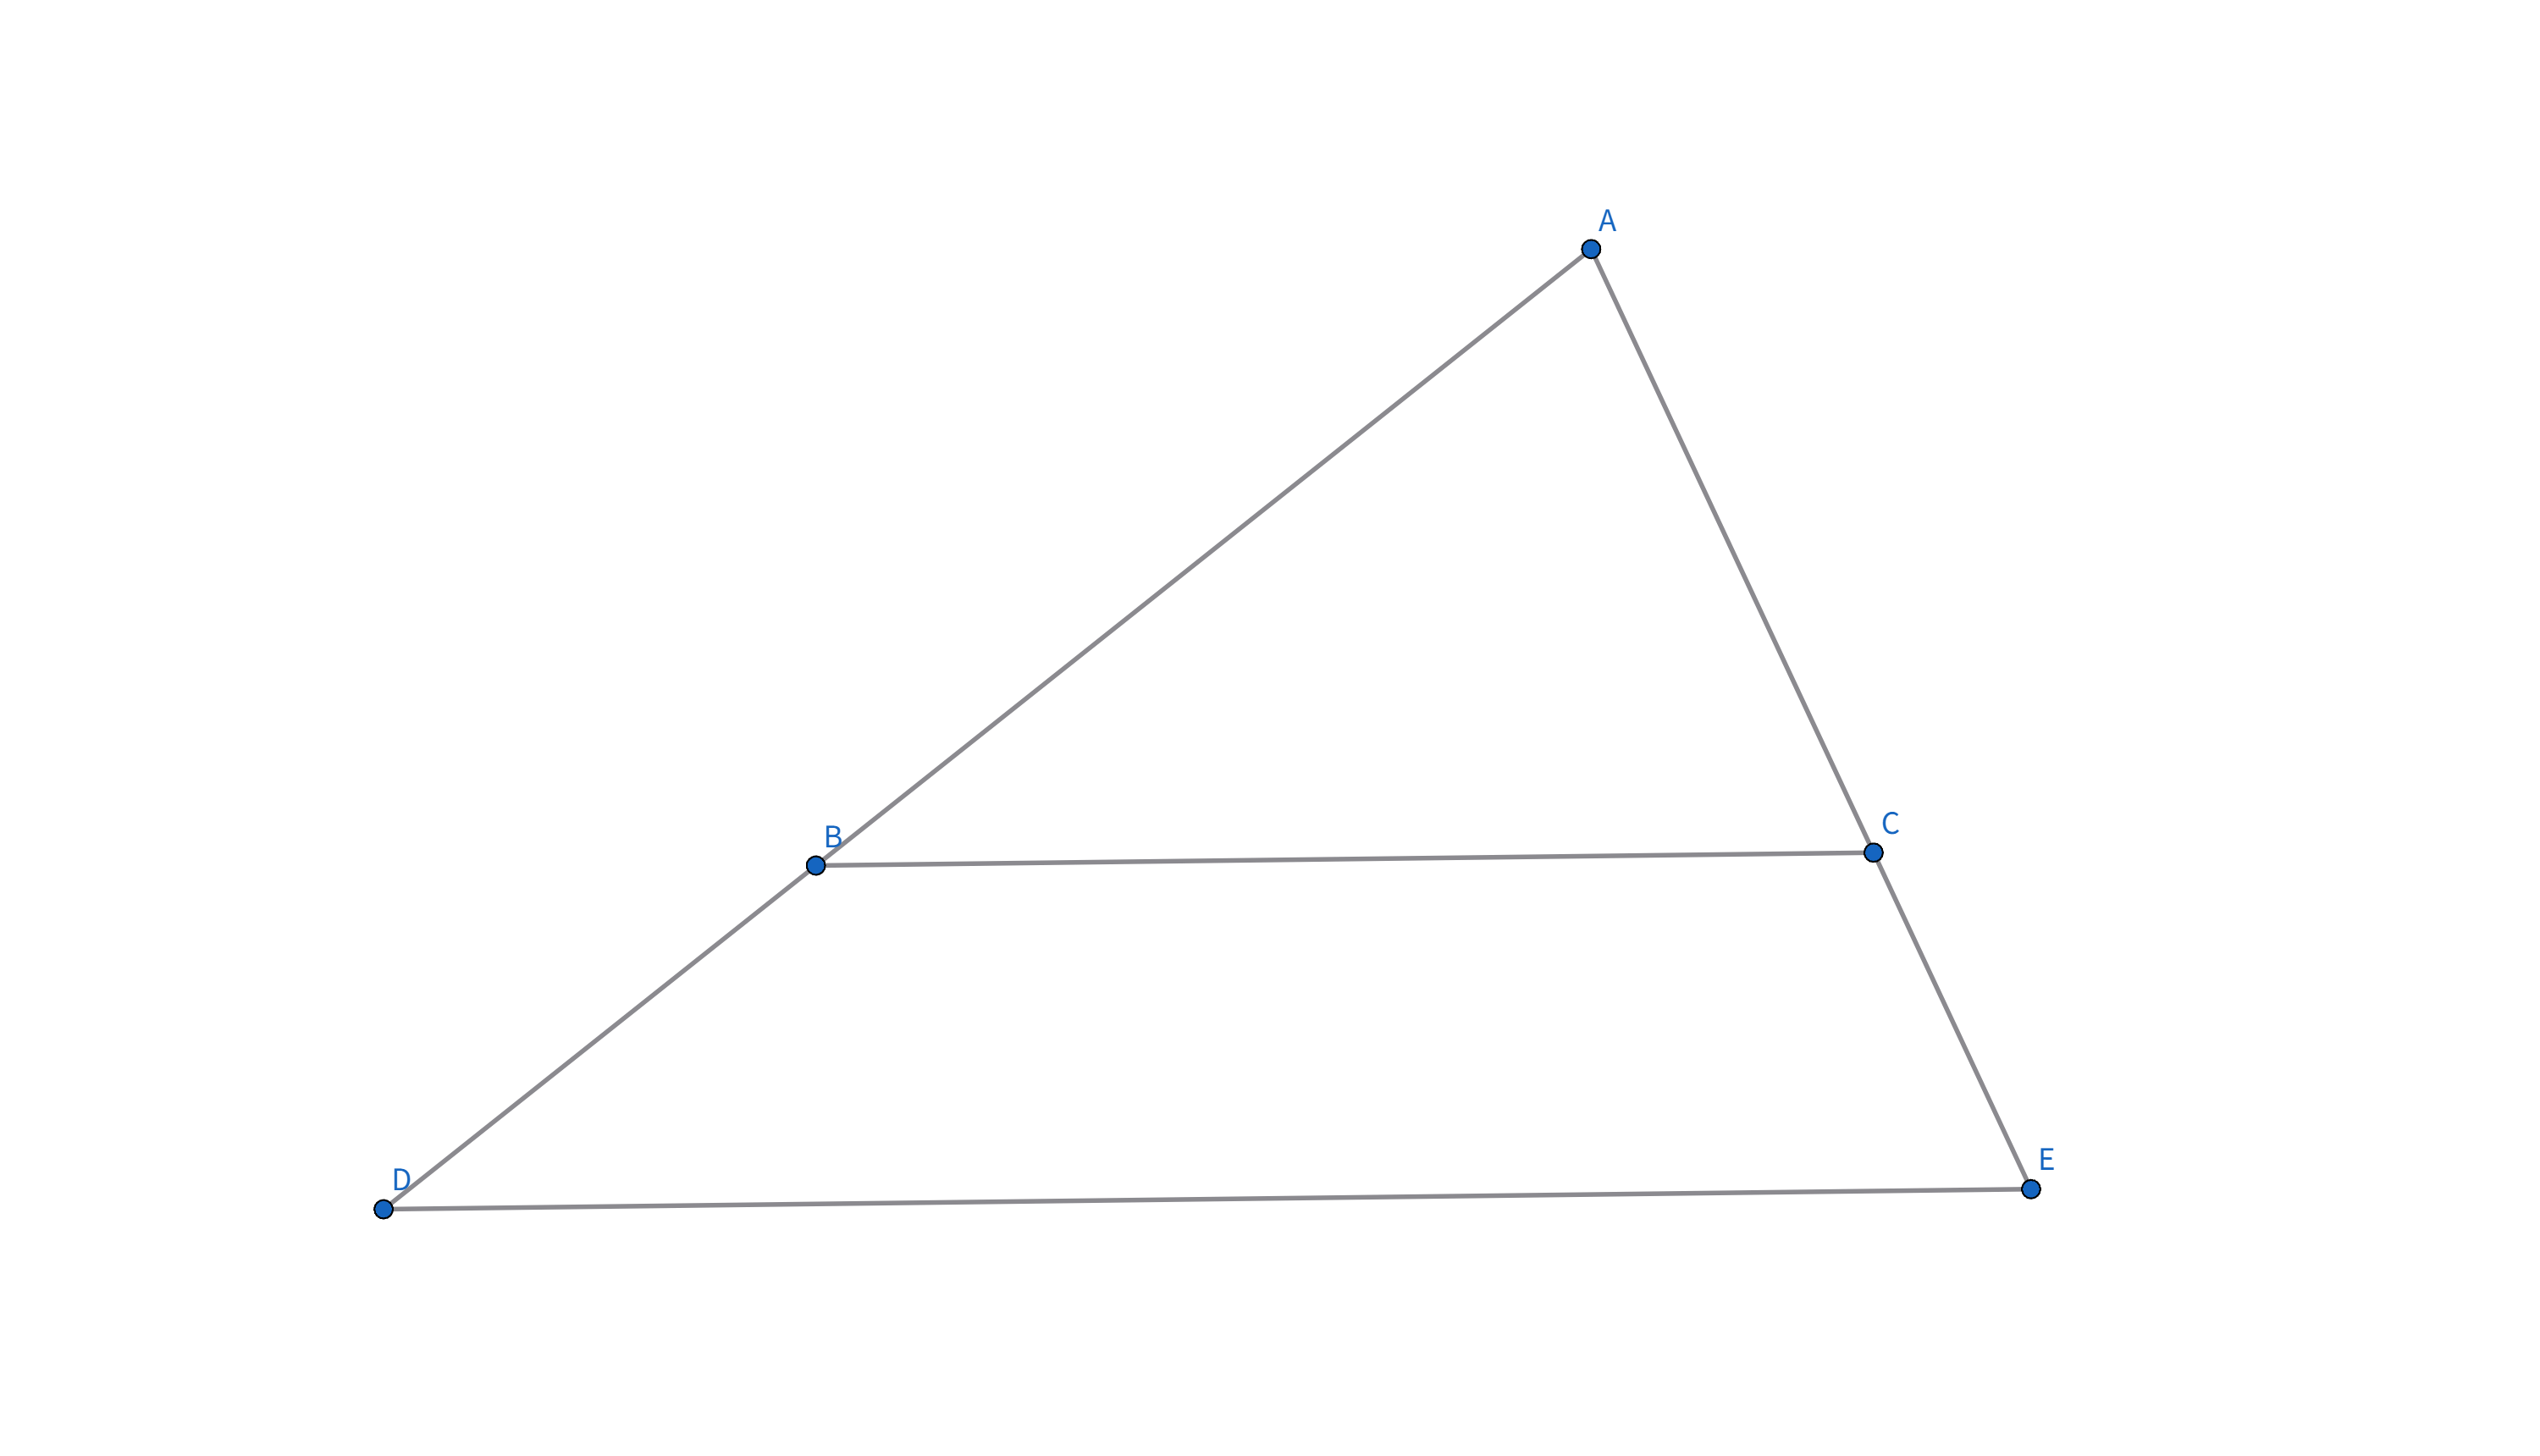
\includegraphics[width=0.8\linewidth]{figures/平行相似.png}
    \caption{平行相似}
    \end{minipage}
    \hfill % 添加一些水平间距
    \begin{minipage}[t]{0.45\textwidth}
    \centering
    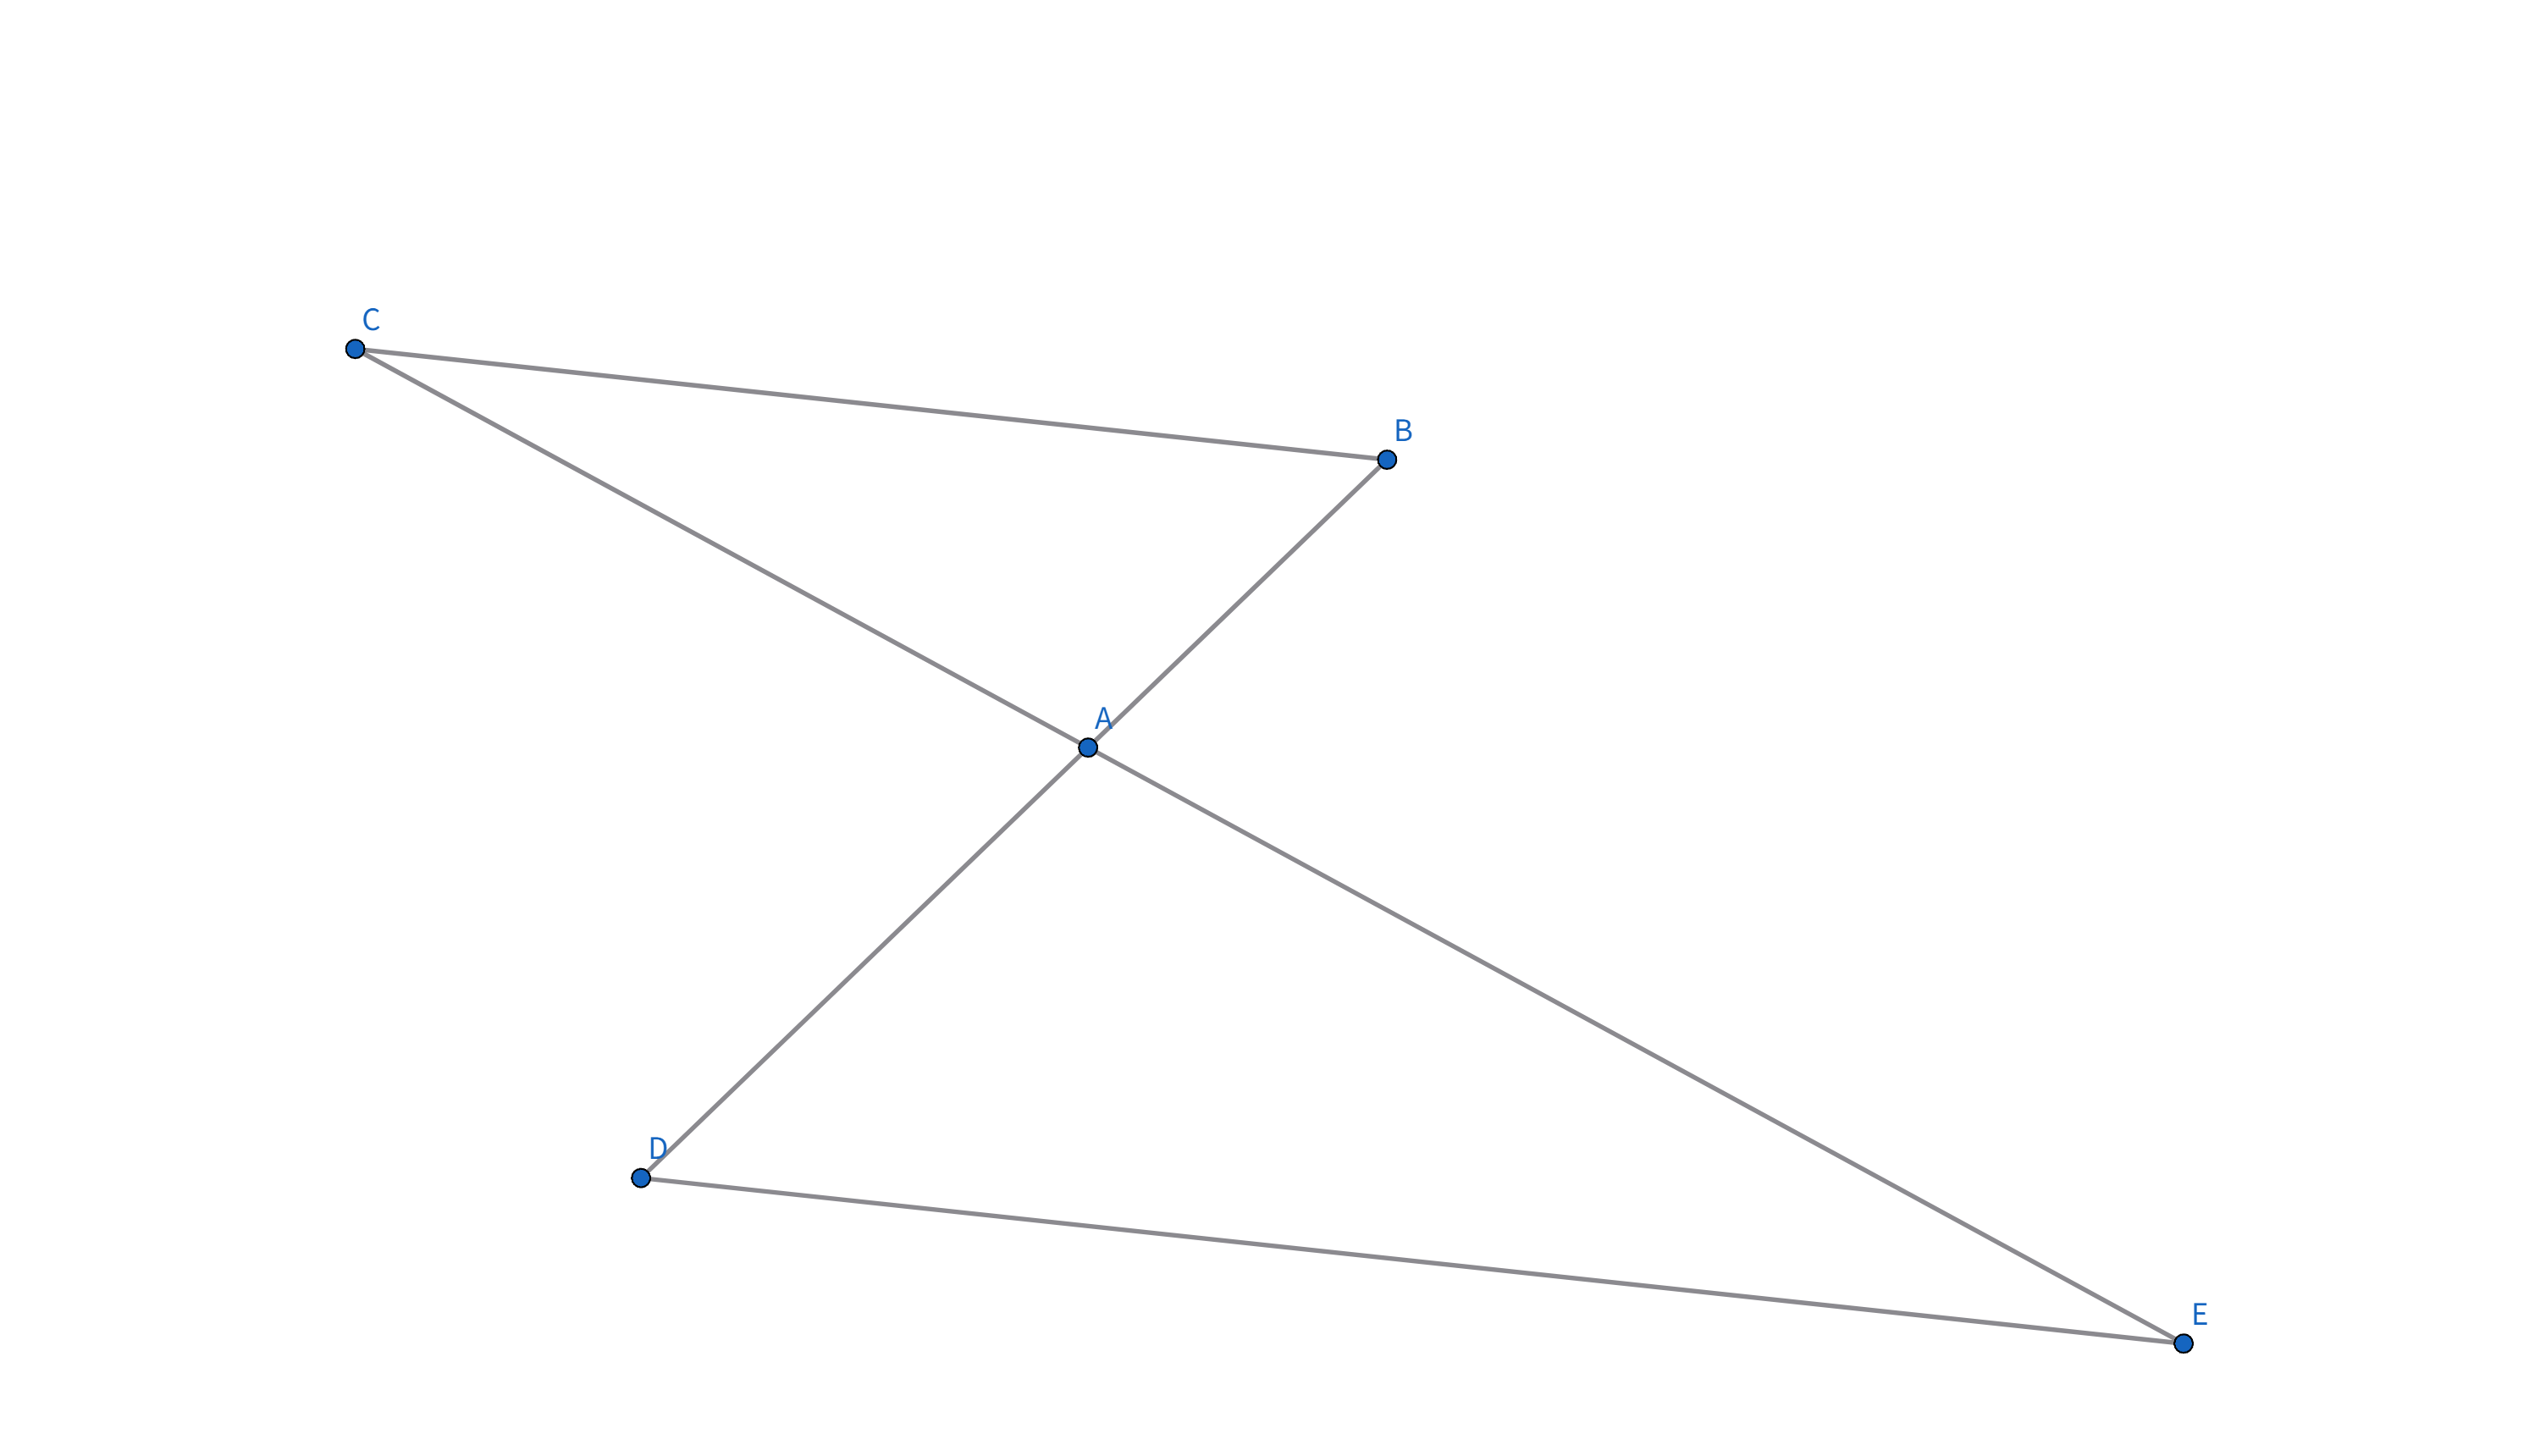
\includegraphics[width=0.8\linewidth]{figures/平行相似2.png}
    \caption{平行相似}
    \end{minipage}
\end{figure}

\begin{figure}[h]
    \centering
    \hfill % 添加一些水平间距
    \begin{minipage}[t]{0.45\textwidth}
    \centering
    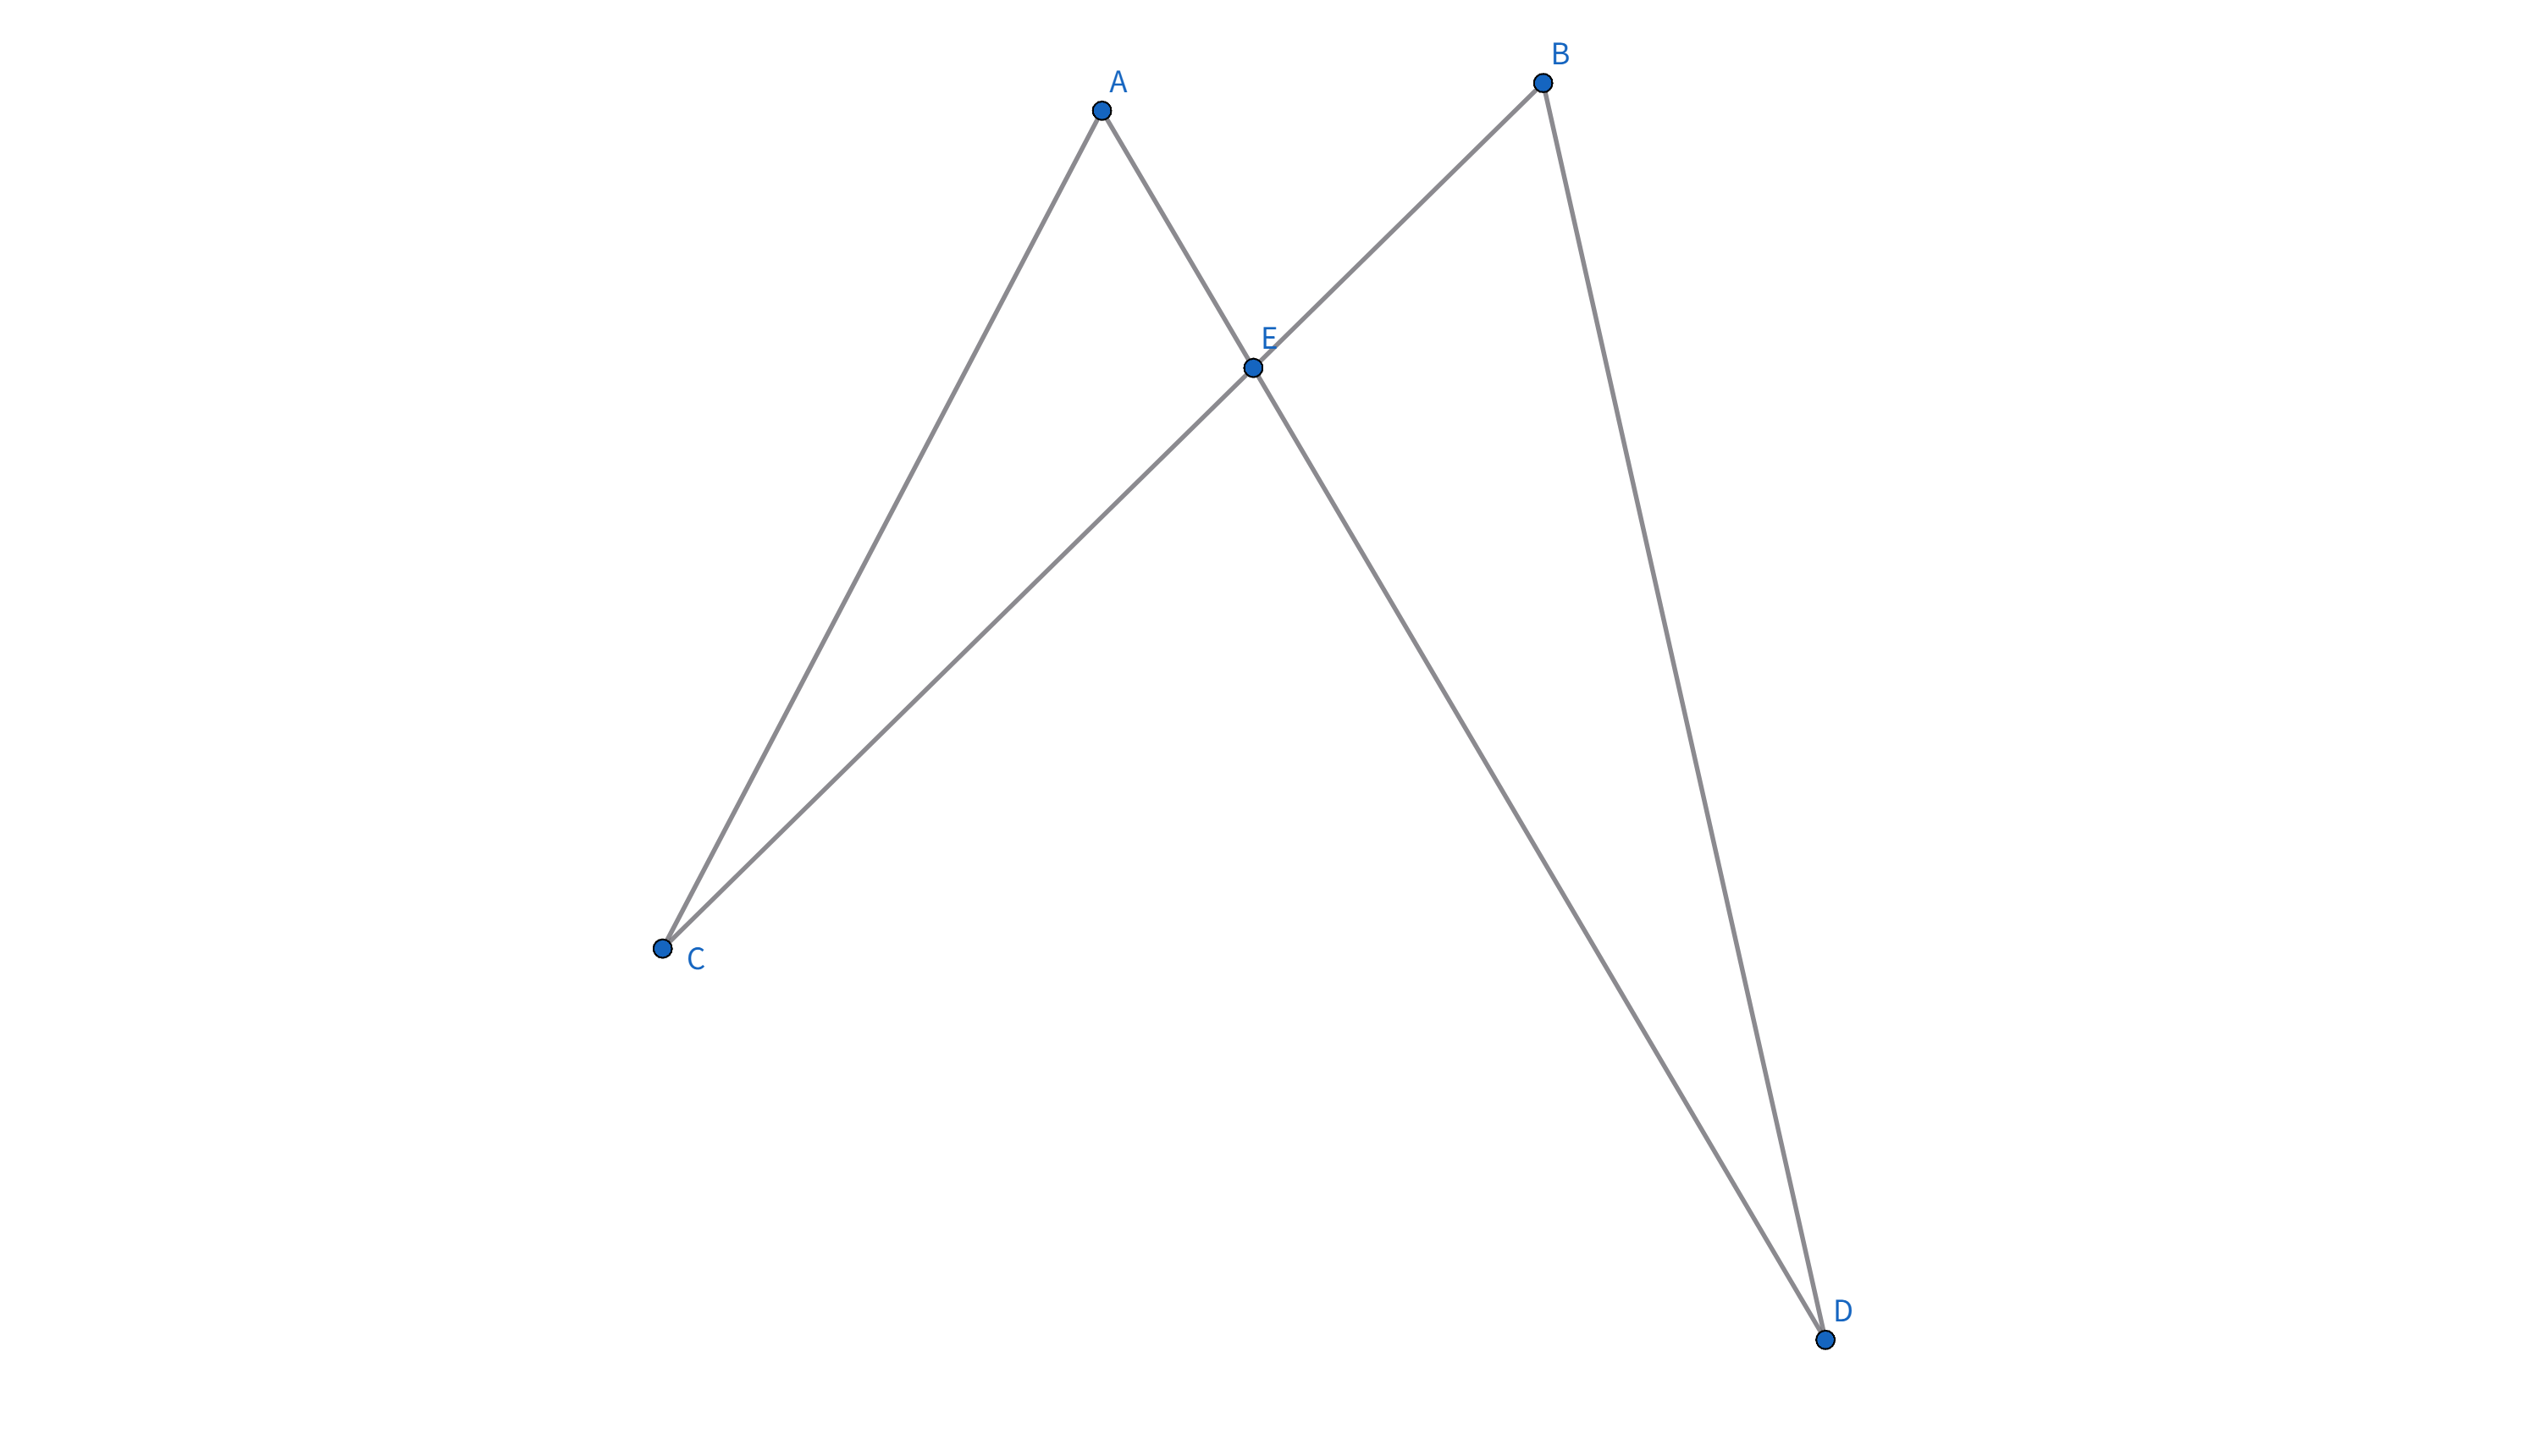
\includegraphics[width=0.8\linewidth]{figures/蝴蝶型相似.png}
    \caption{蝴蝶型相似}
    \end{minipage}
    \hfill % 添加一些水平间距
    \begin{minipage}[t]{0.45\textwidth}
    \centering
    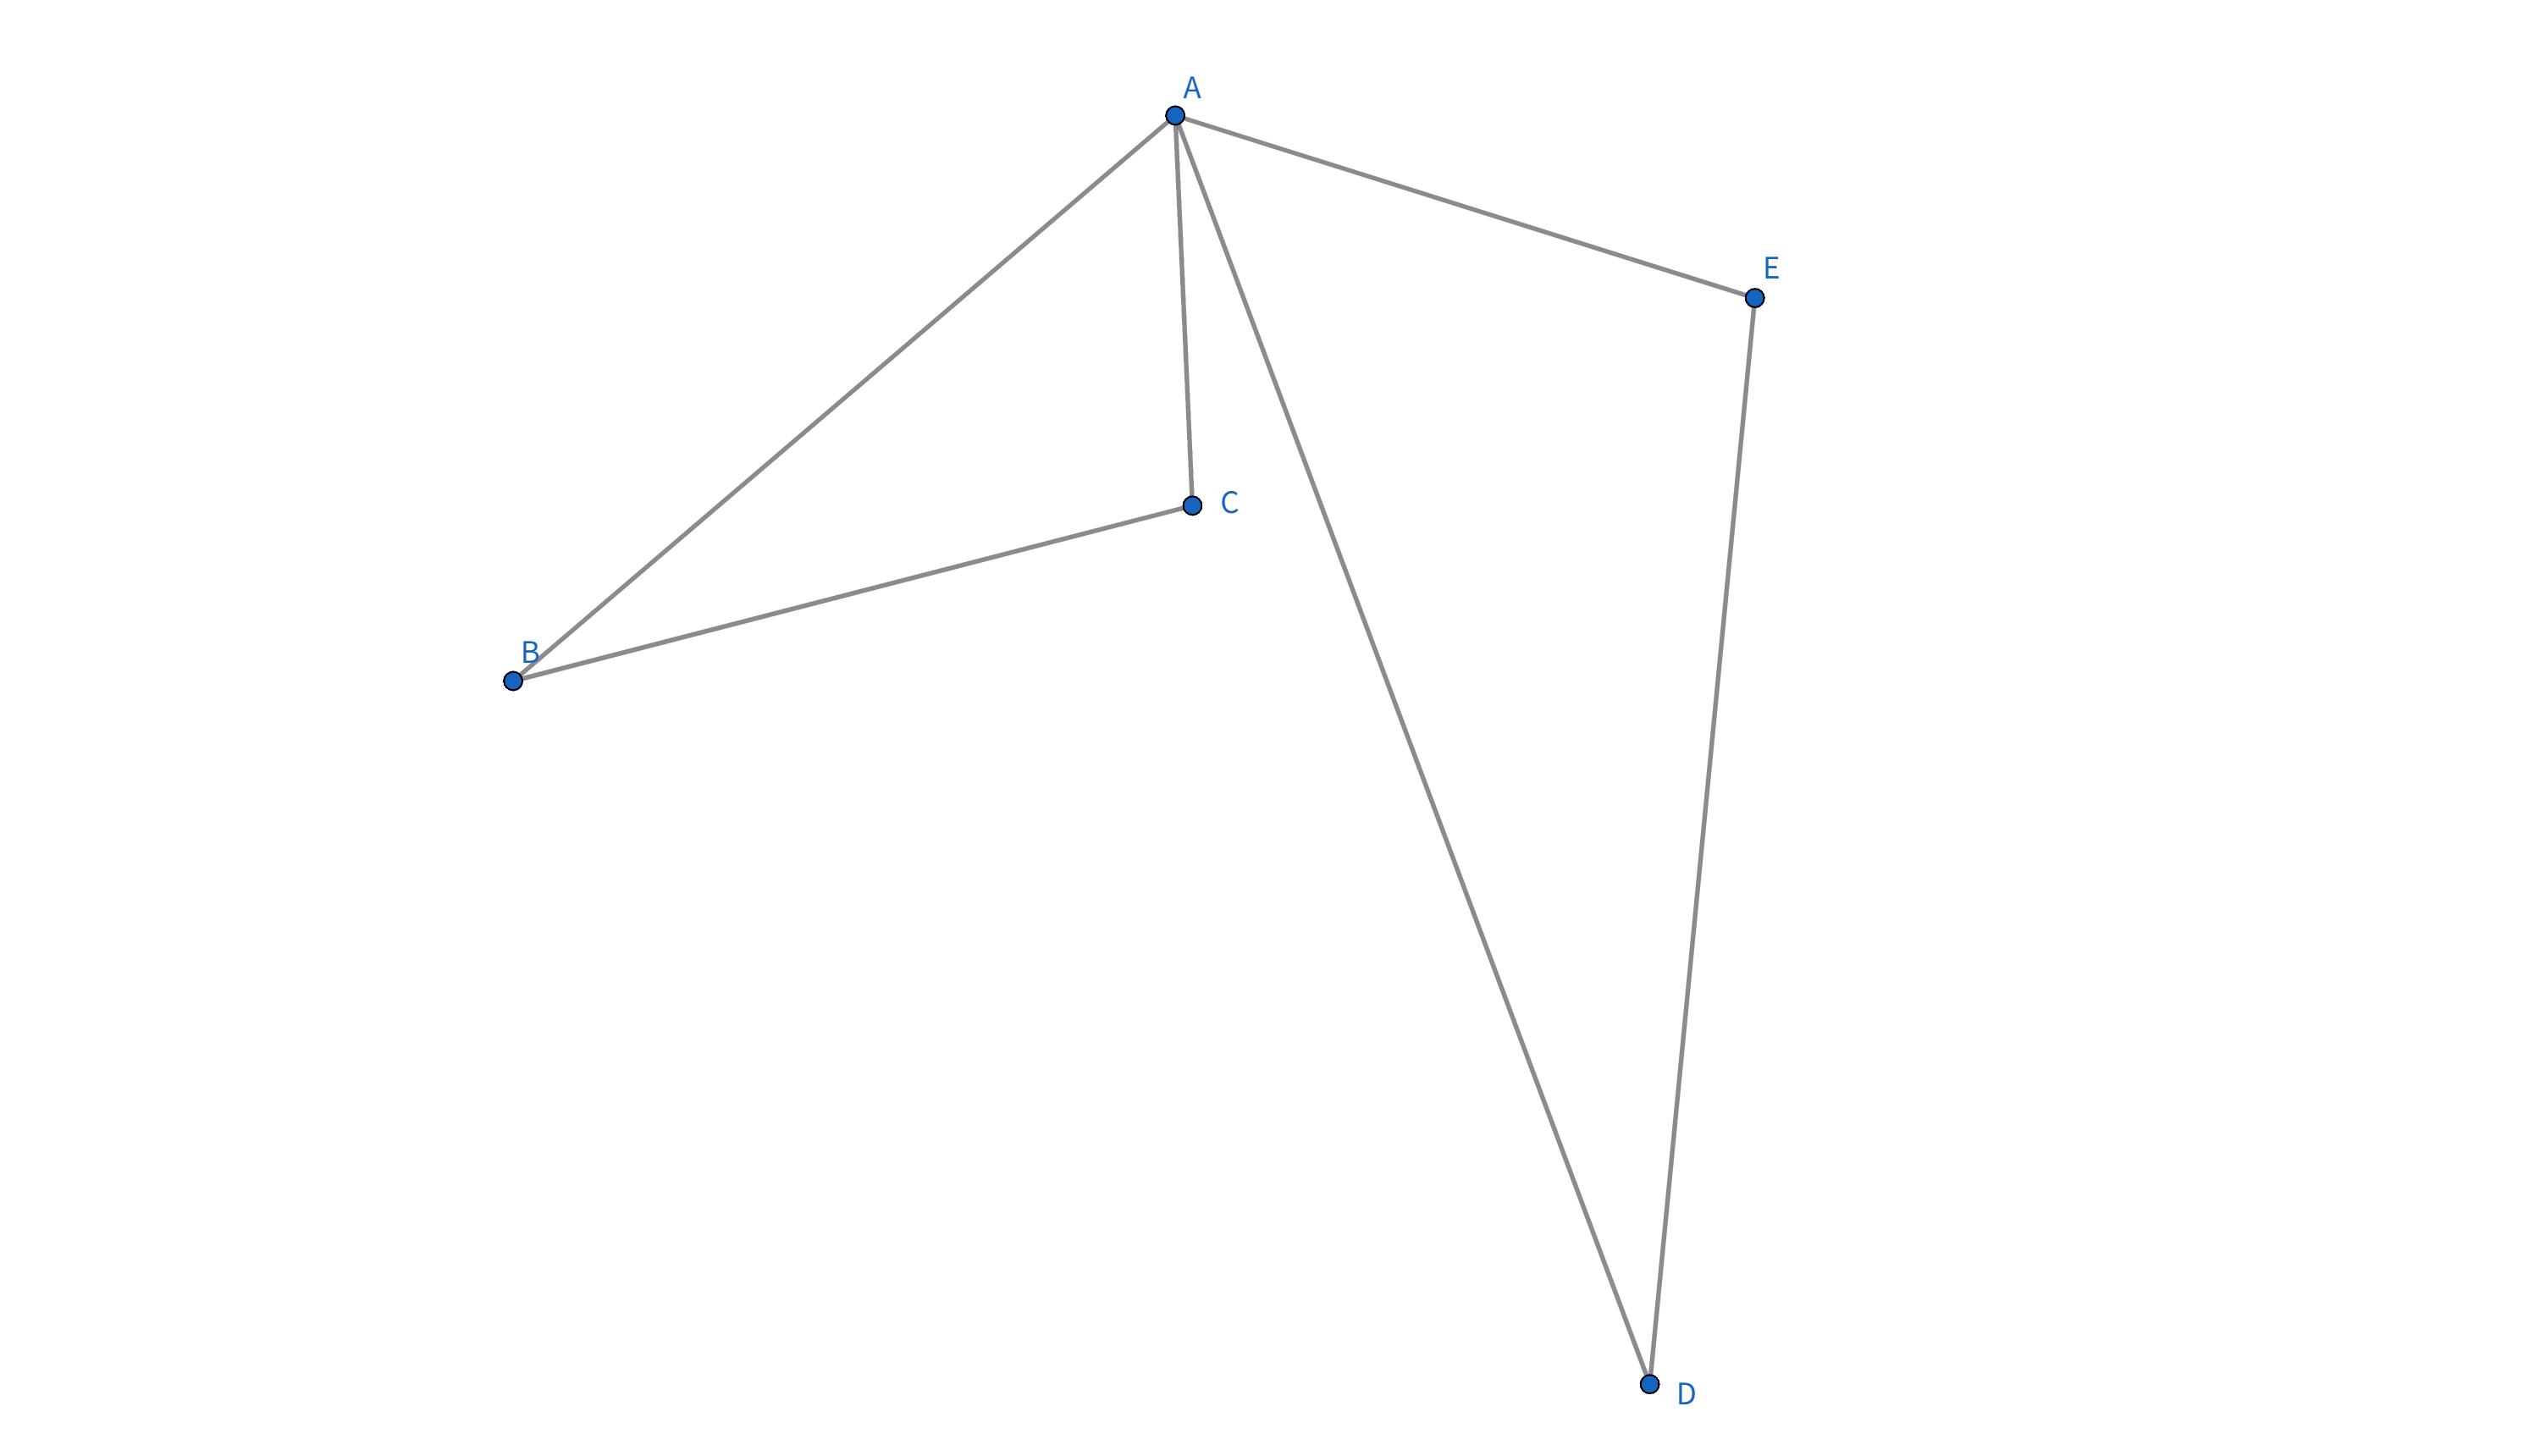
\includegraphics[width=0.8\linewidth]{figures/旋转型相似.png}
    \caption{旋转型相似}
    \end{minipage}
\end{figure}


\begin{figure}[h]
    \centering
    \hfill % 添加一些水平间距
    \begin{minipage}[t]{0.45\textwidth}
    \centering
    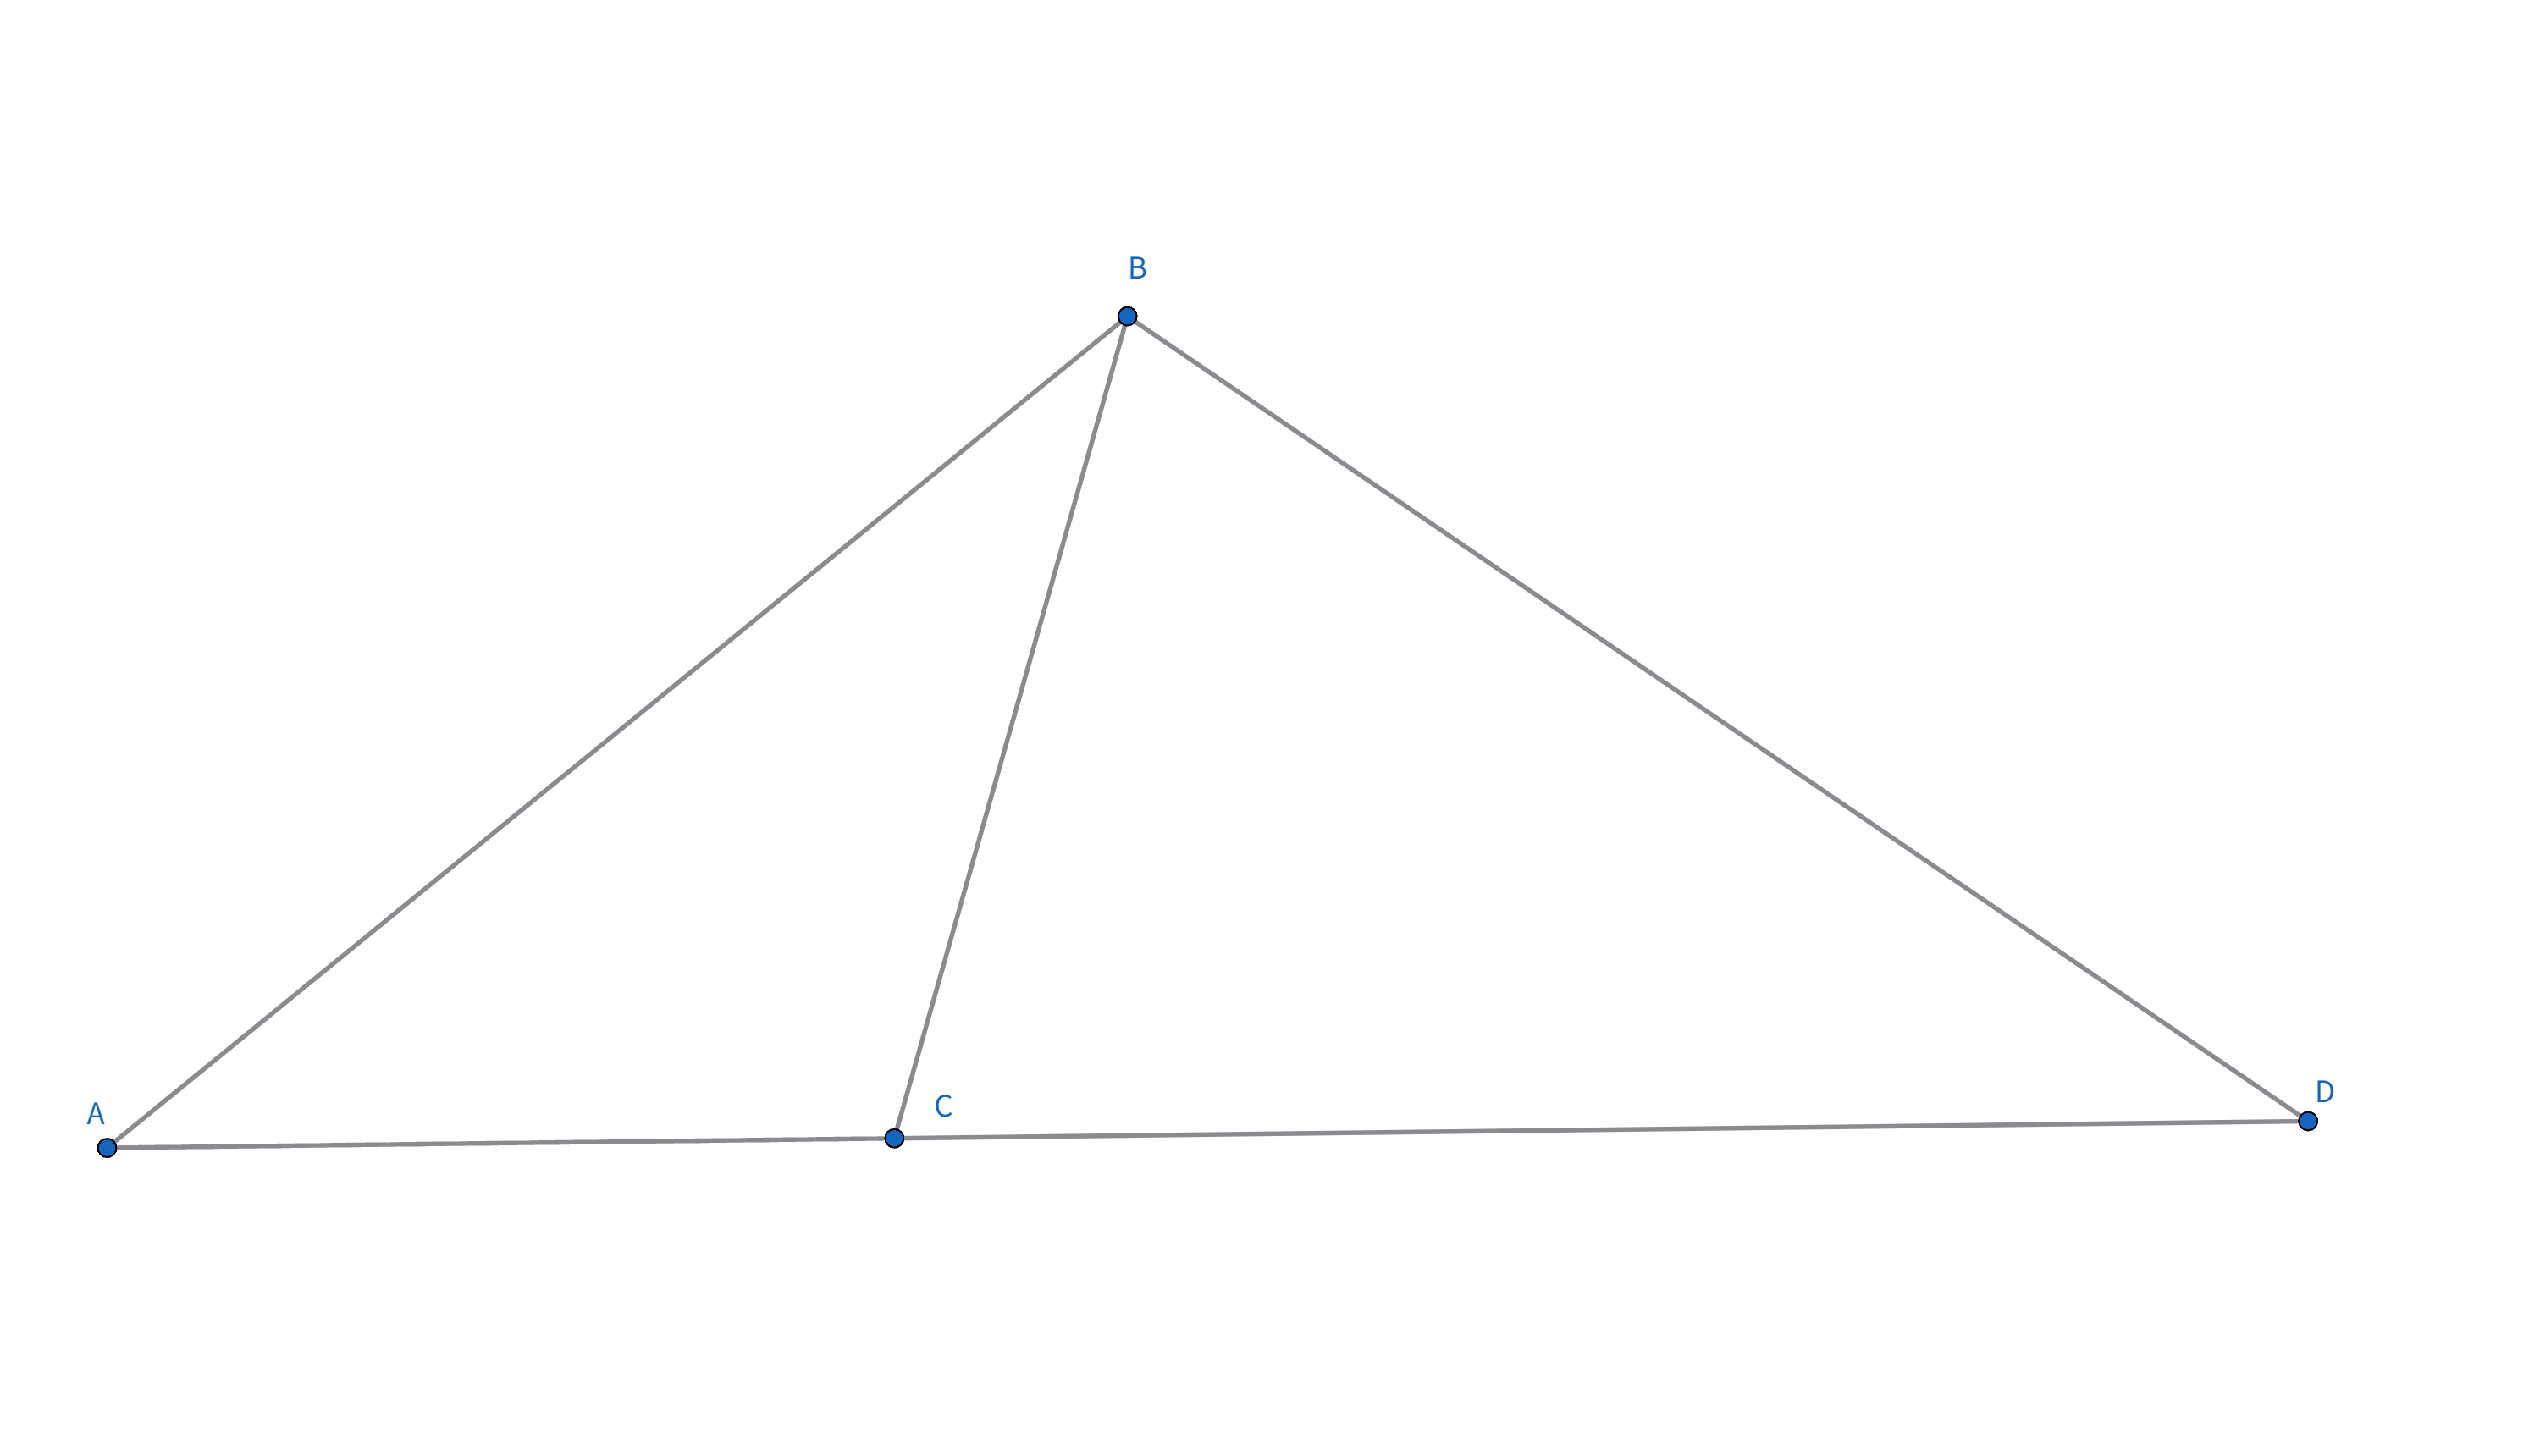
\includegraphics[width=0.8\linewidth]{figures/子母型相似.png}
    \caption{子母型相似}
    \end{minipage}
    \hfill % 添加一些水平间距
    \begin{minipage}[t]{0.45\textwidth}
    \centering
    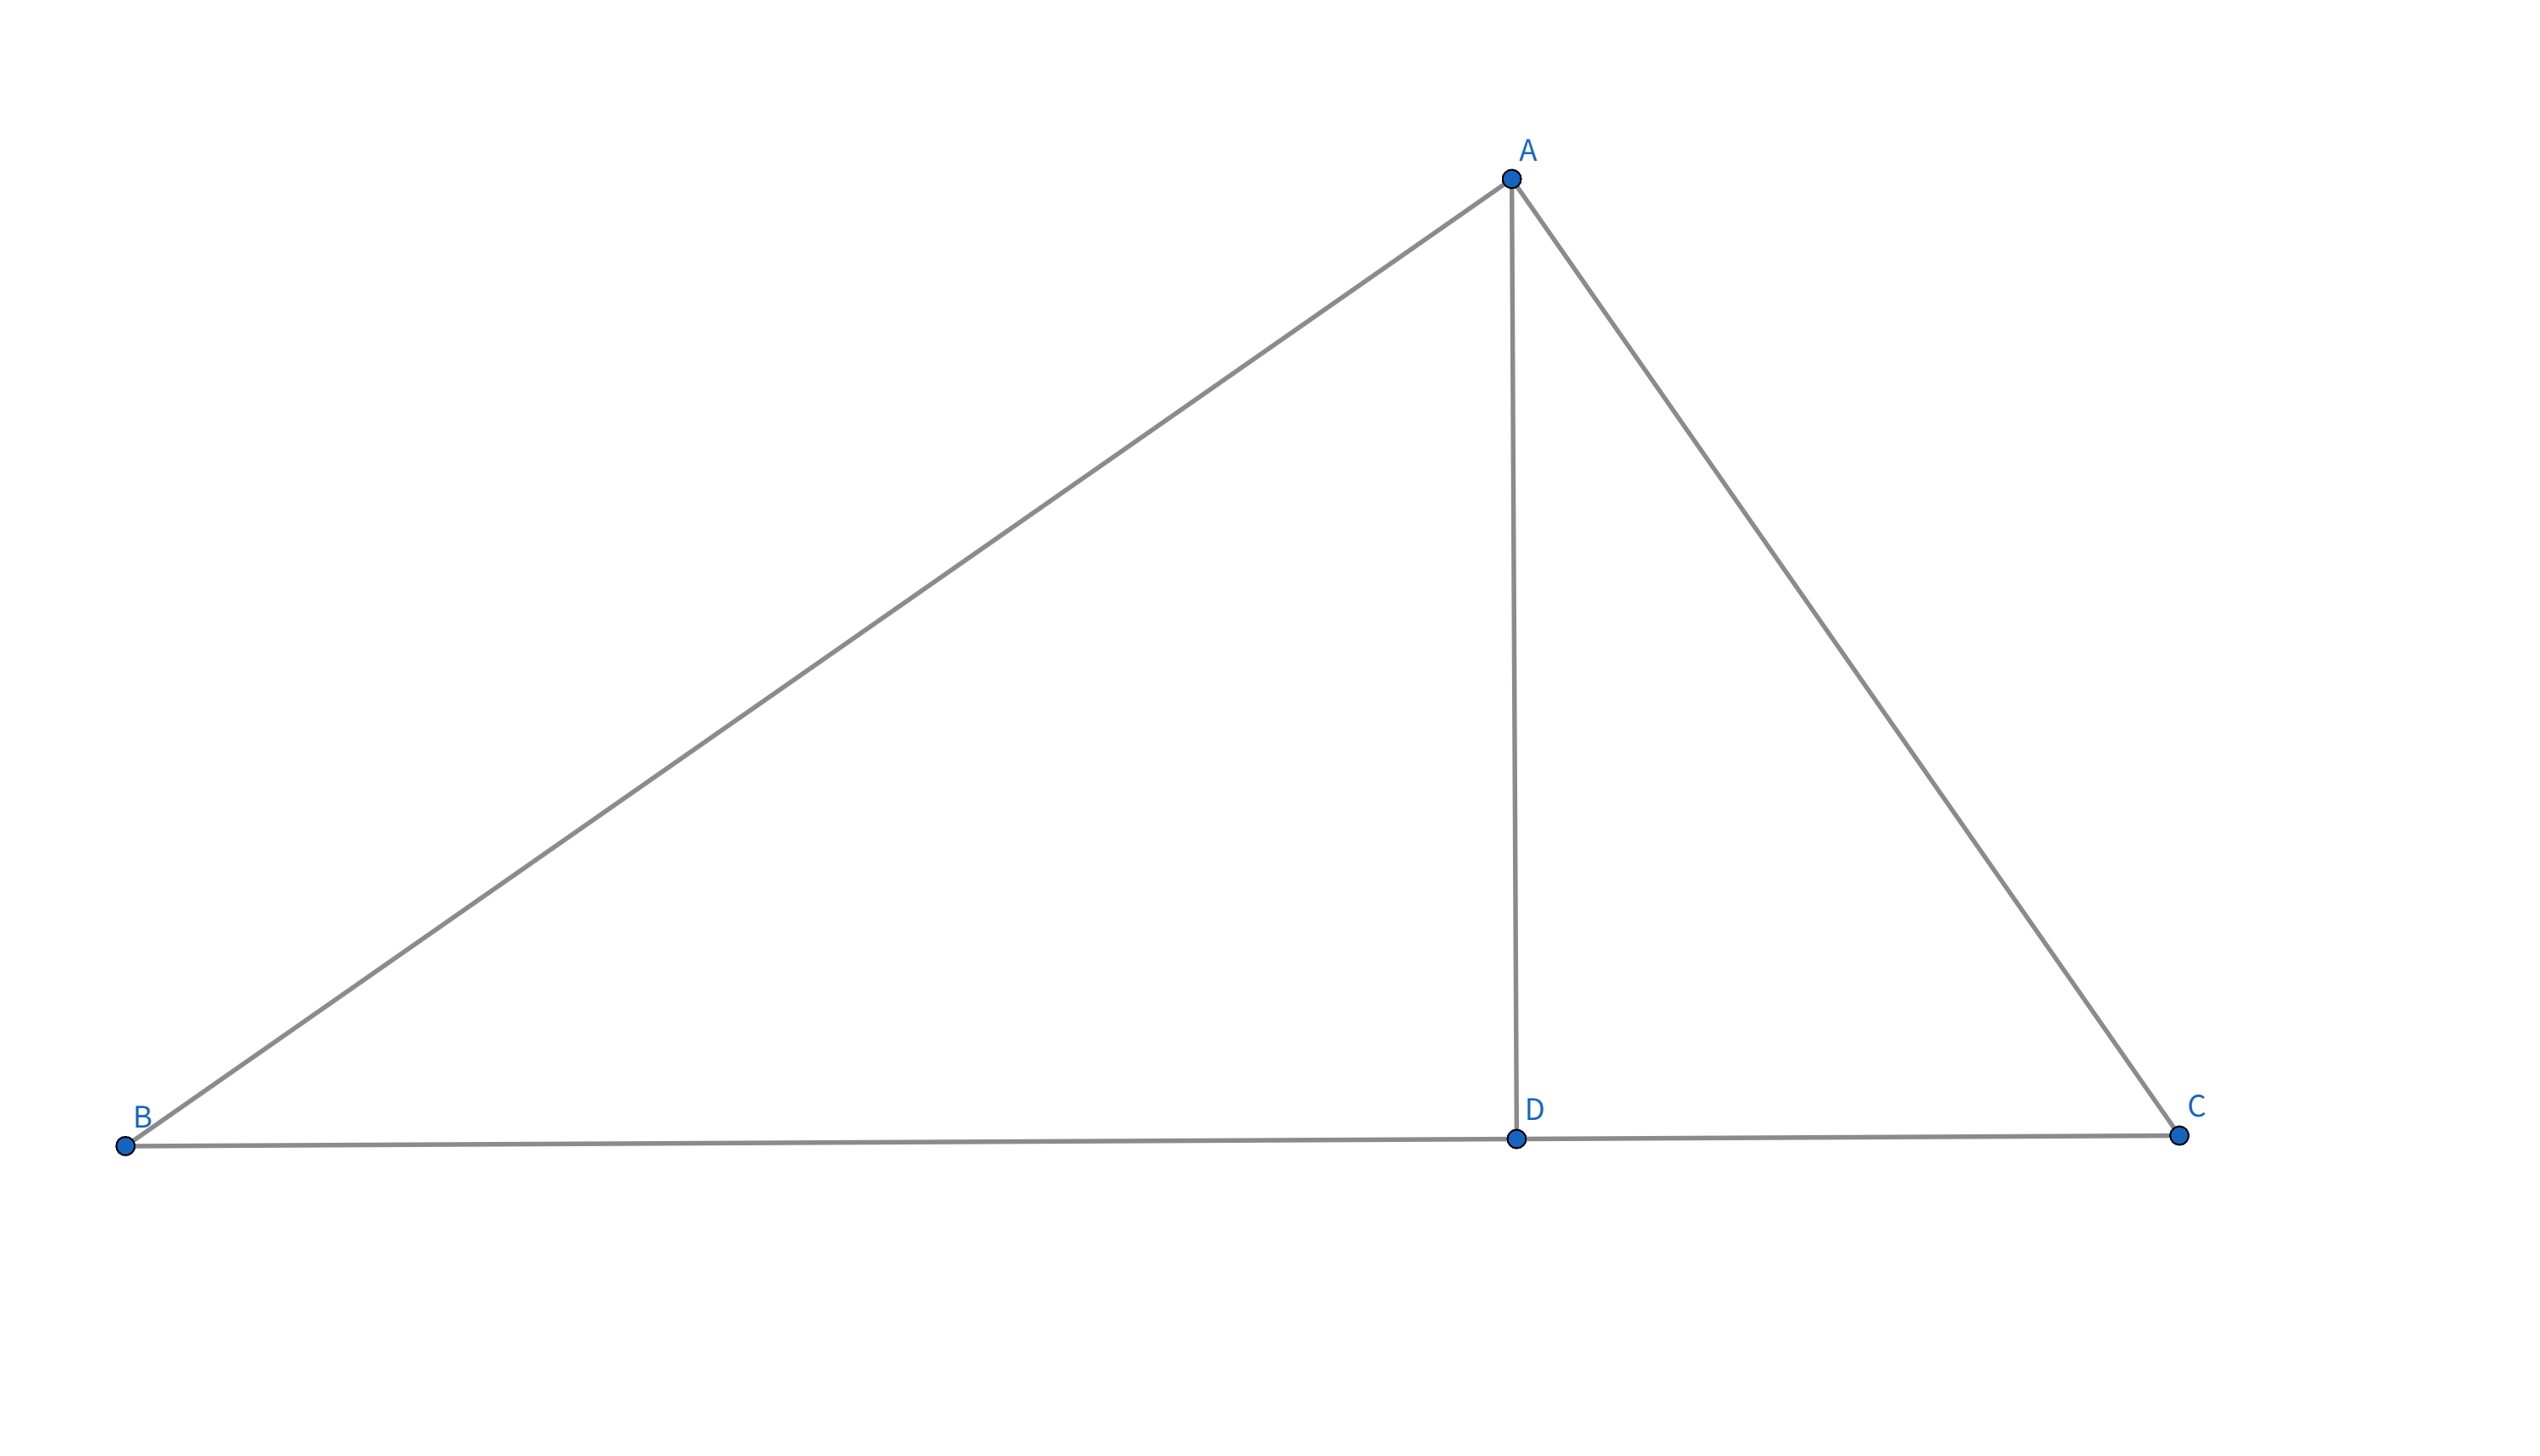
\includegraphics[width=0.8\linewidth]{figures/射影定理.png}
    \caption{直角子母型相似}
    \end{minipage}
\end{figure}




\subsection{射影定理}
\begin{theorem}[射影定理]
    在直角$\triangle ABC$中,AD为斜边BC上的垂线,D为垂足。有下面等式成立:
    $$
    \begin{aligned}
    BA^2 &= BD\cdot BC,\\ 
    CA^2 &= CD\cdot CB,\\
    AD^2 &= DB\cdot DC
    \end{aligned}
    $$
\end{theorem}
\begin{figure}[h]
    \centering
    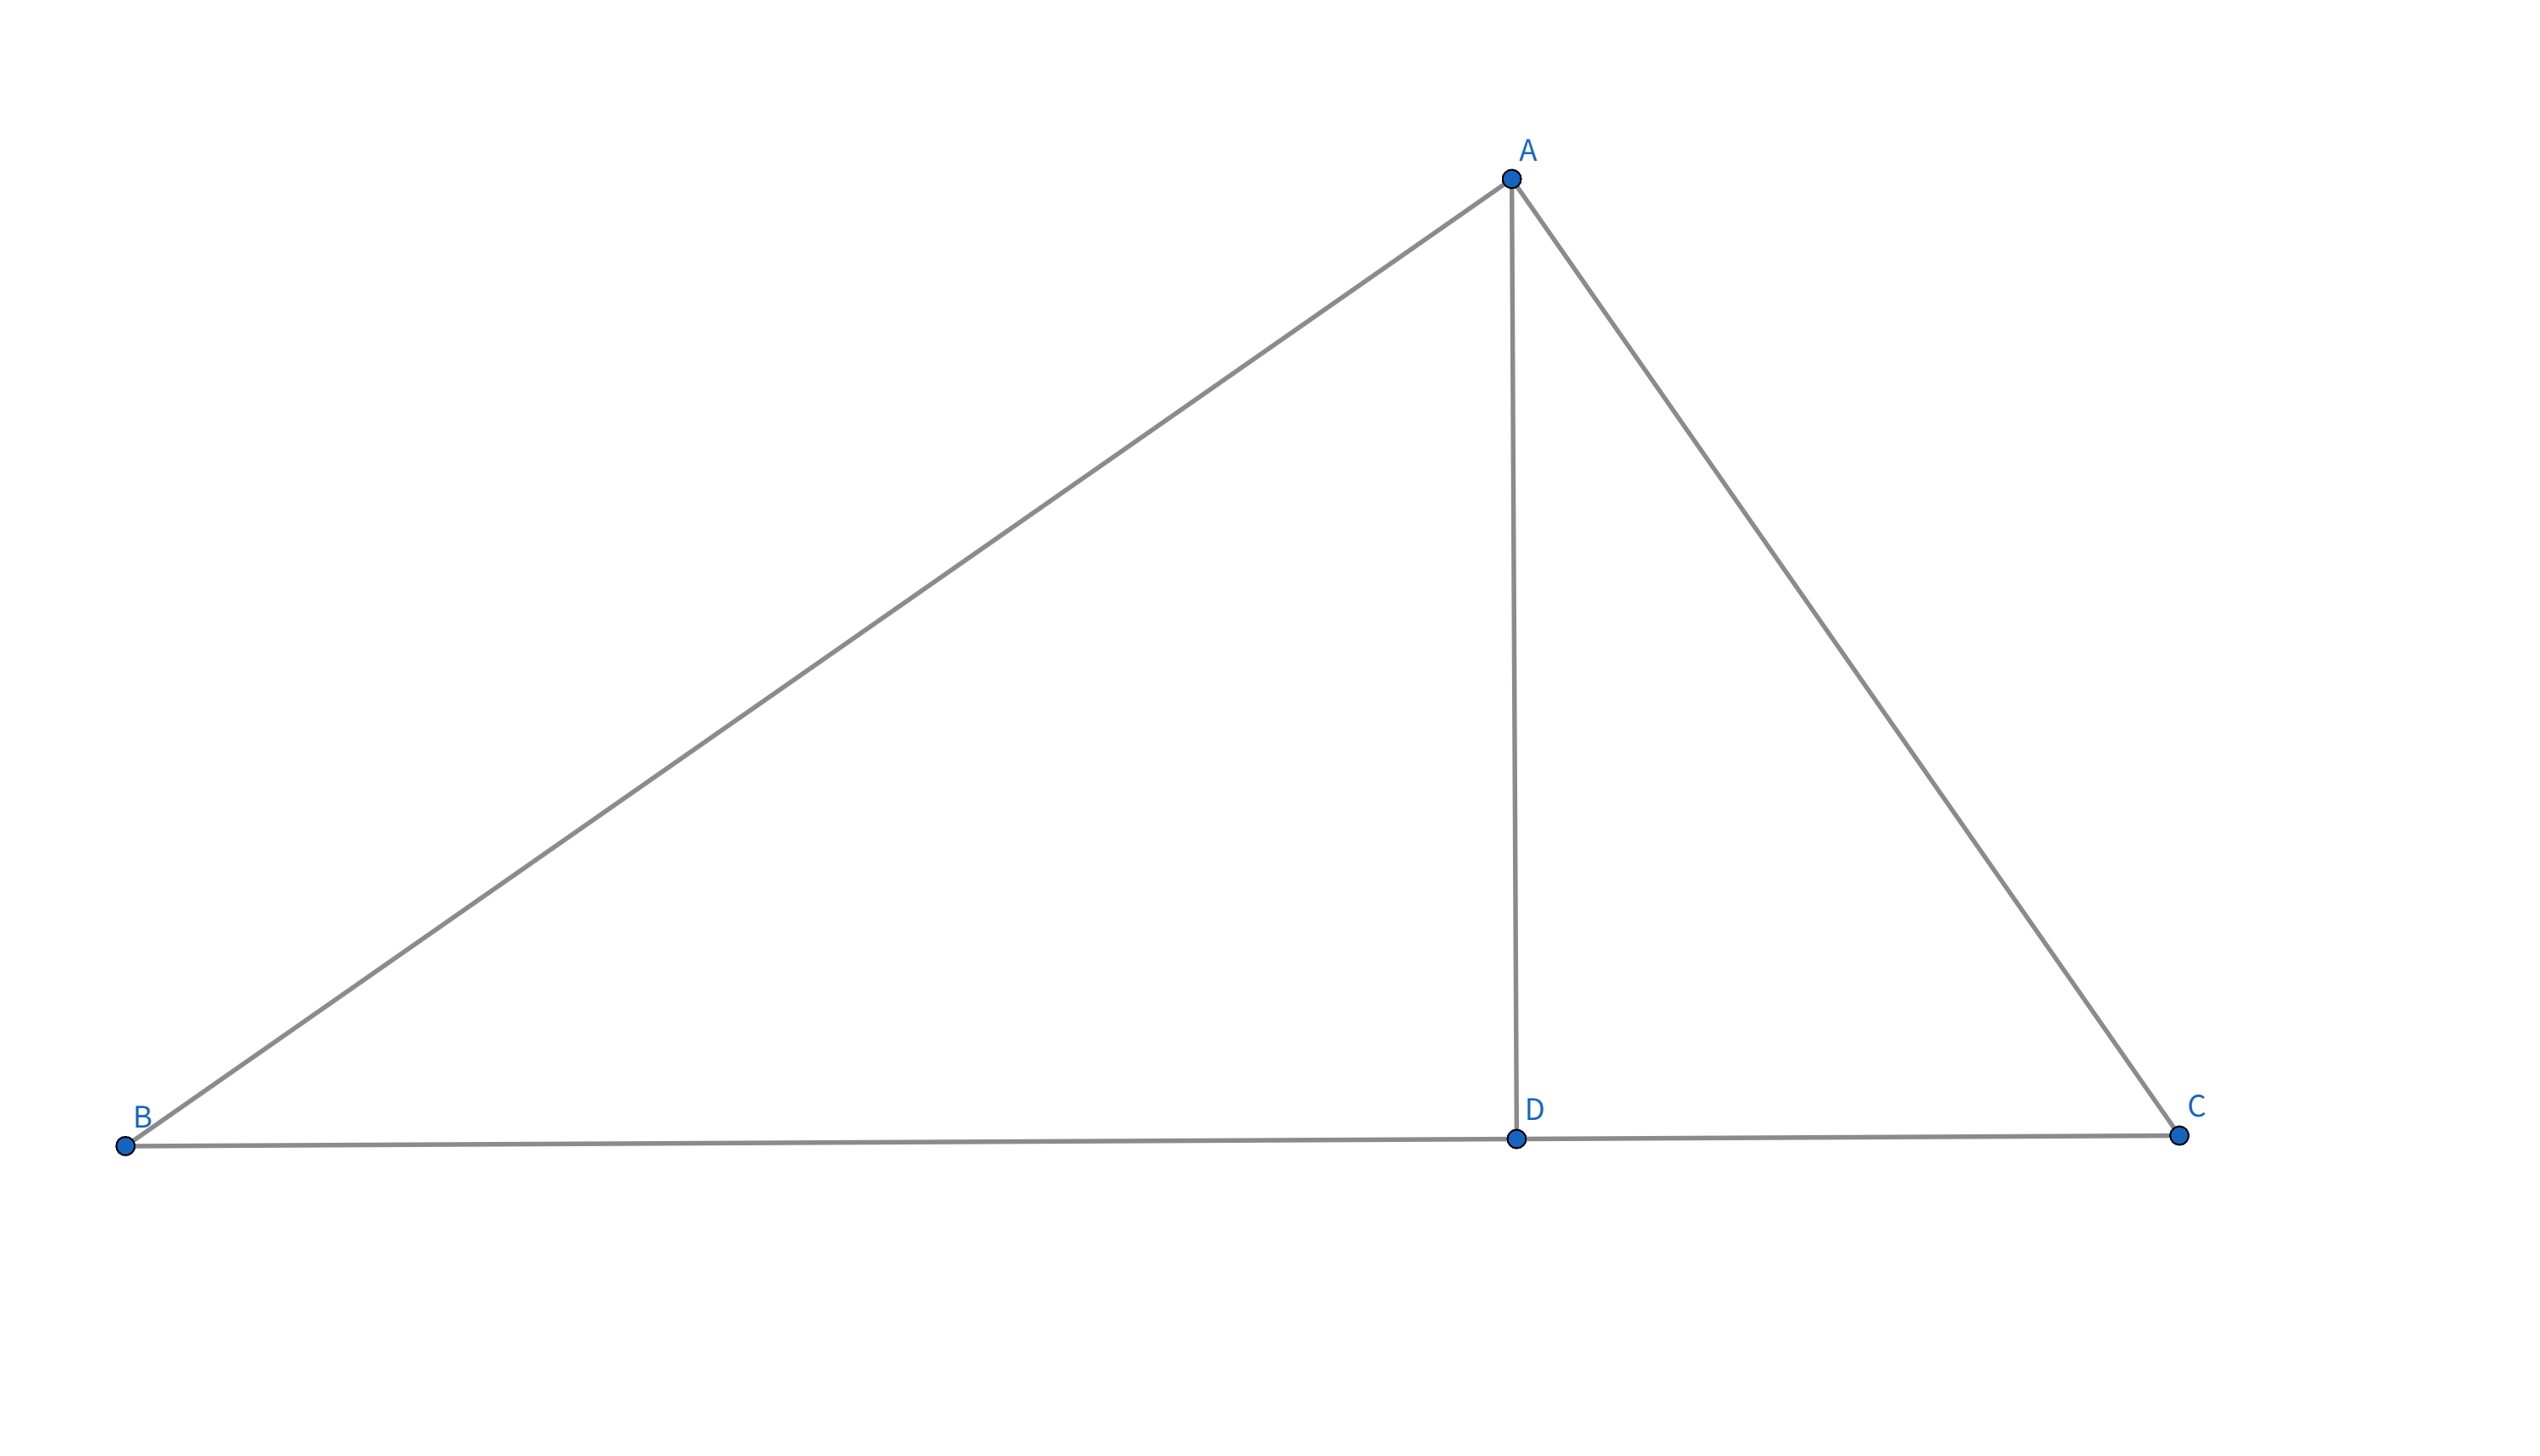
\includegraphics[width=0.8\linewidth]{figures/射影定理.png}
    \caption{射影定理}
    % \label{fig:enter-label}
\end{figure}

% \include{Lessons/Basic/圆.tex}
% \part{三点共线与三线共点}
%---------------------------------------------------
\section{梅涅劳斯定理}
\begin{theorem}[梅涅劳斯(Menelaus)定理]
    如果一条不通过A、B、C三点的直线与$\triangle ABC$ 的边BC、CA、AB所在直线分别交于X、Y、Z,则 
    $$\frac{A Z}{Z B} \cdot \frac{B X}{X C} \cdot \frac{C Y}{Y A}=1.$$ 
\end{theorem}


\begin{figure}[H]
    \centering
    \begin{minipage}[t]{0.45\textwidth}
        \centering
        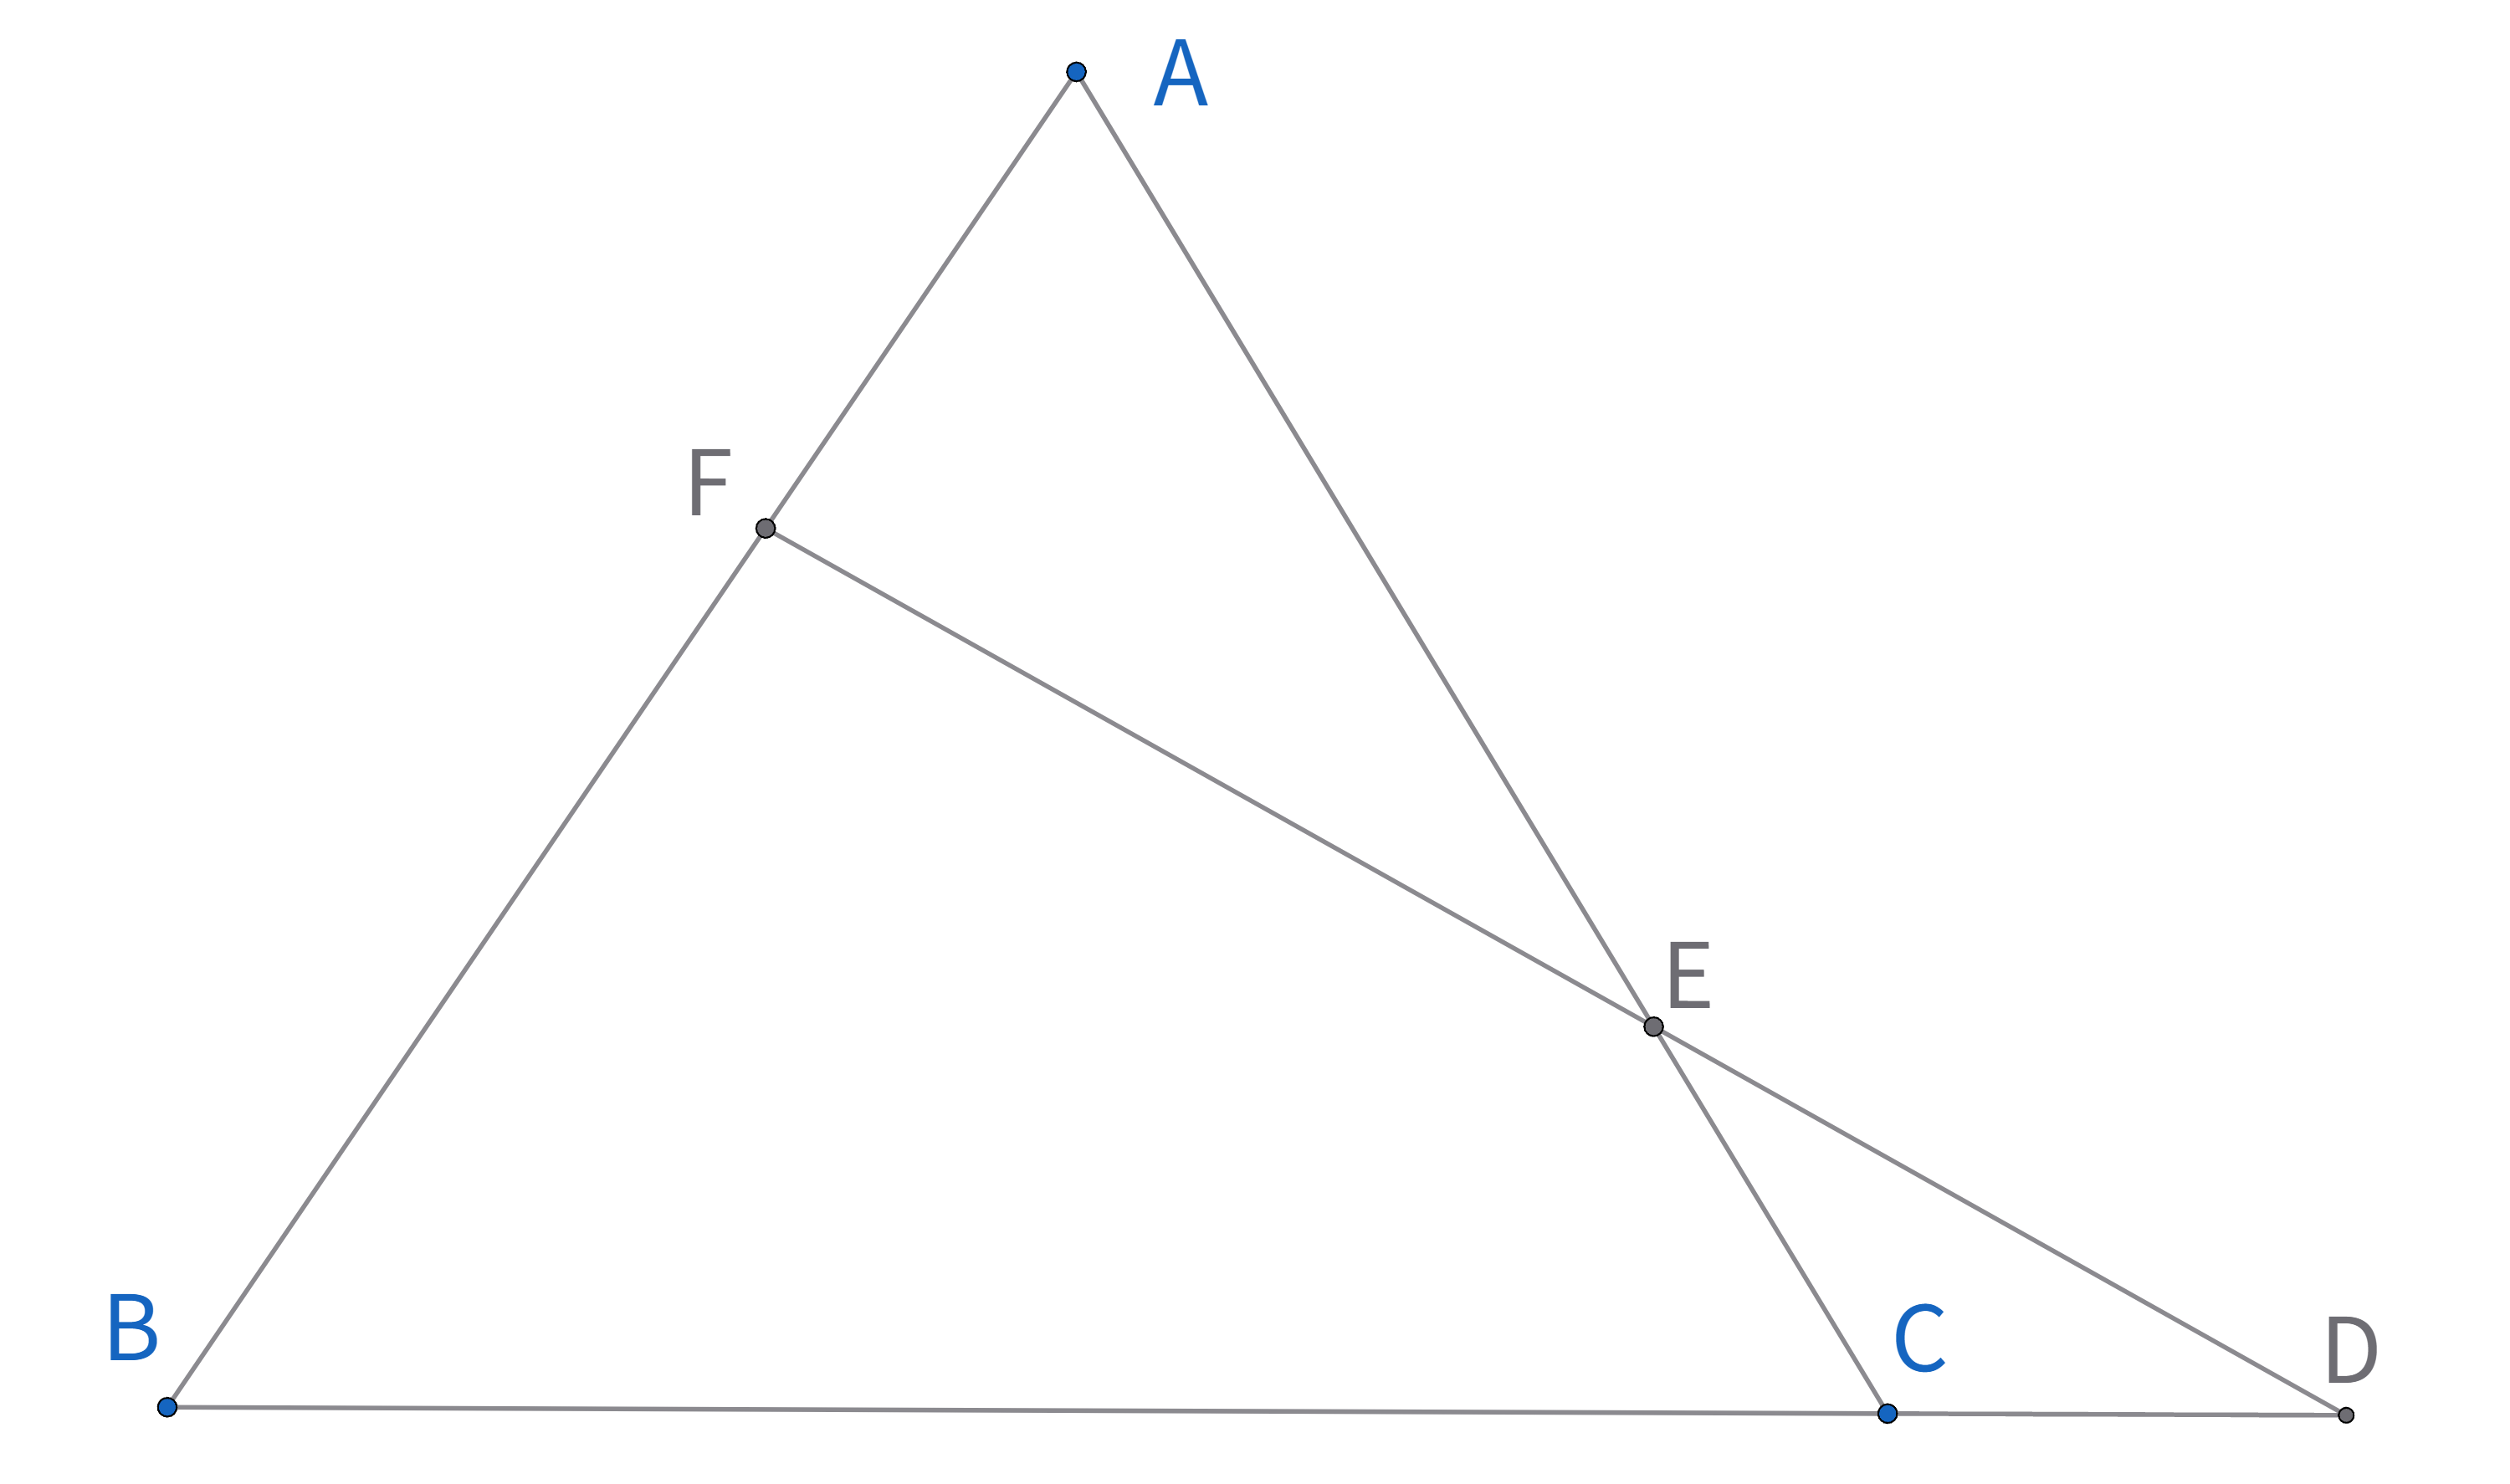
\includegraphics[width=\linewidth]{figures/menelaus1.png}
    \end{minipage}
    \hfill % 添加一些水平间距
    \begin{minipage}[t]{0.45\textwidth}
    \centering
    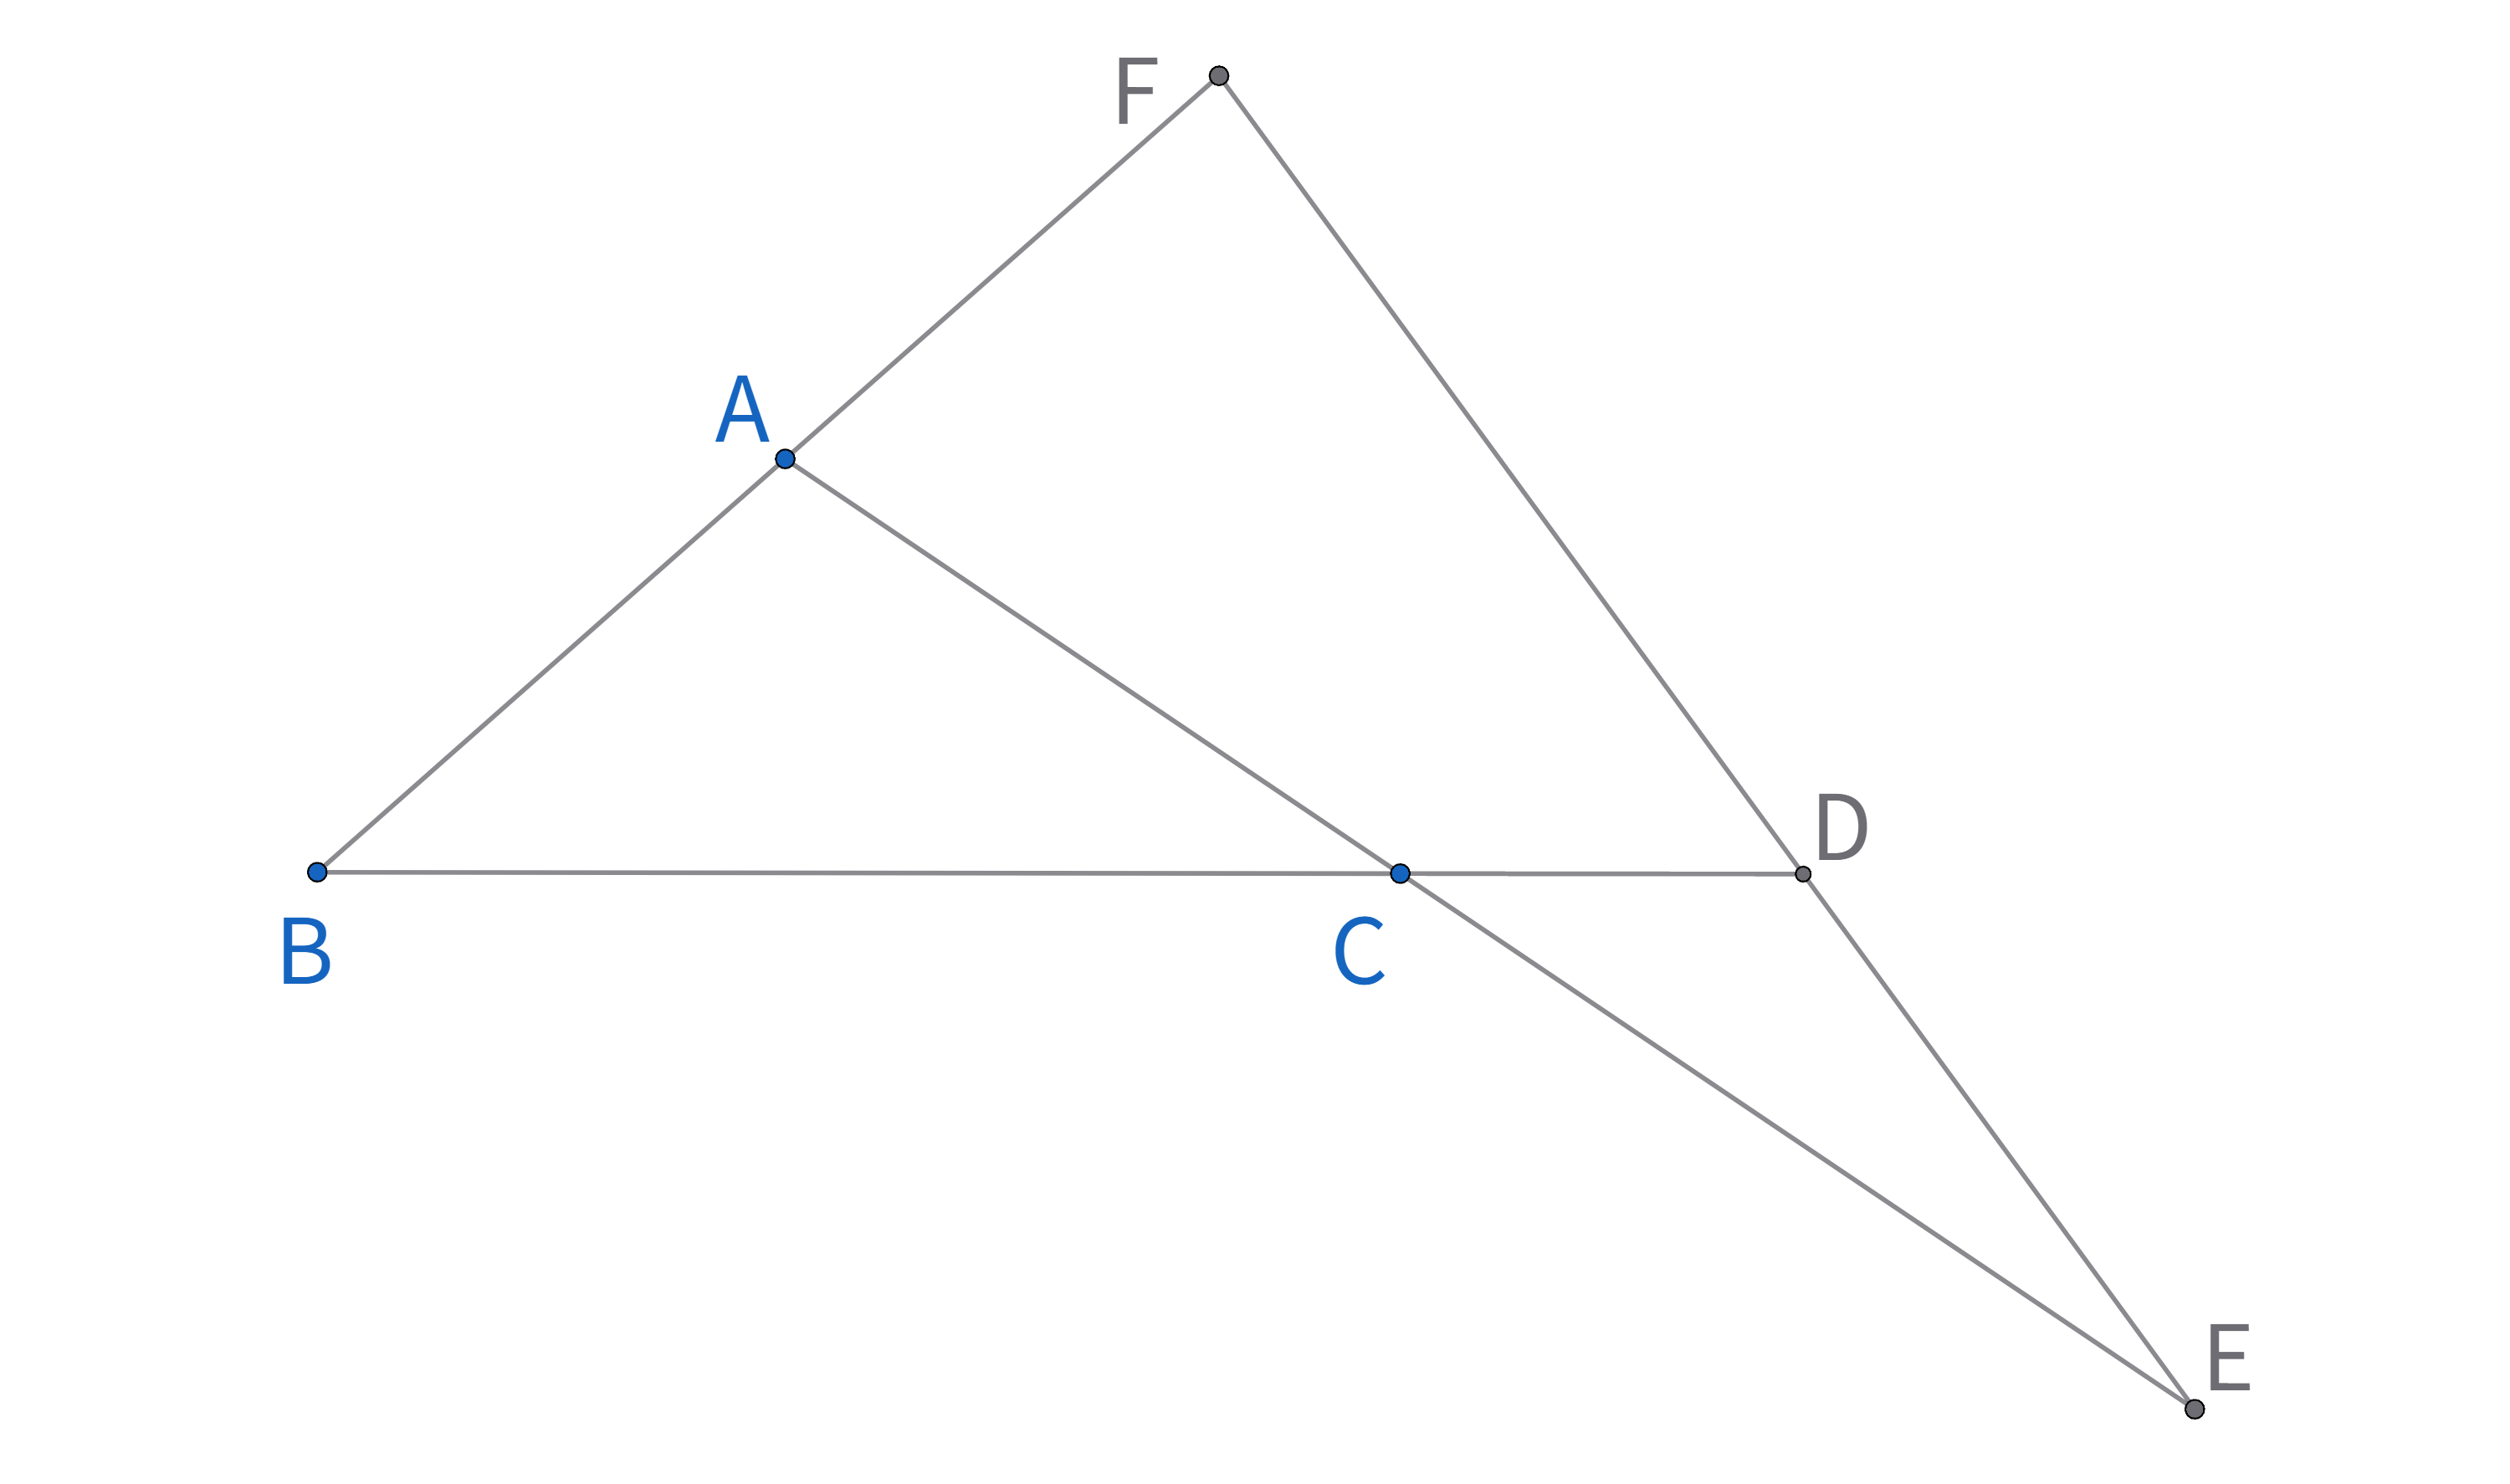
\includegraphics[width=\linewidth]{figures/menelaus2.png}
    \end{minipage}
    \caption{两种情形的梅涅劳斯定理}
\end{figure}


\begin{theorem}[梅涅劳斯(Menelaus)逆定理]
如果 $X 、 Y 、 Z$ 中有偶数个点在 $\triangle A B C$ 的三边上,且点 $X 、 Y 、 Z$ 分别为 $\triangle A B C$ 的三边 $B C 、 C A 、 A B$ 所在直线上的点,满足 
$$\frac{A Z}{Z B} \cdot \frac{B X}{X C} \cdot \frac{C Y}{Y A}=1,$$
则 $X 、 Y 、 Z$ 三点共线.
\end{theorem}



\begin{figure}[H]
    \centering
    \hfill % 添加一些水平间距
    \begin{minipage}[t]{0.45\textwidth}
        \centering
        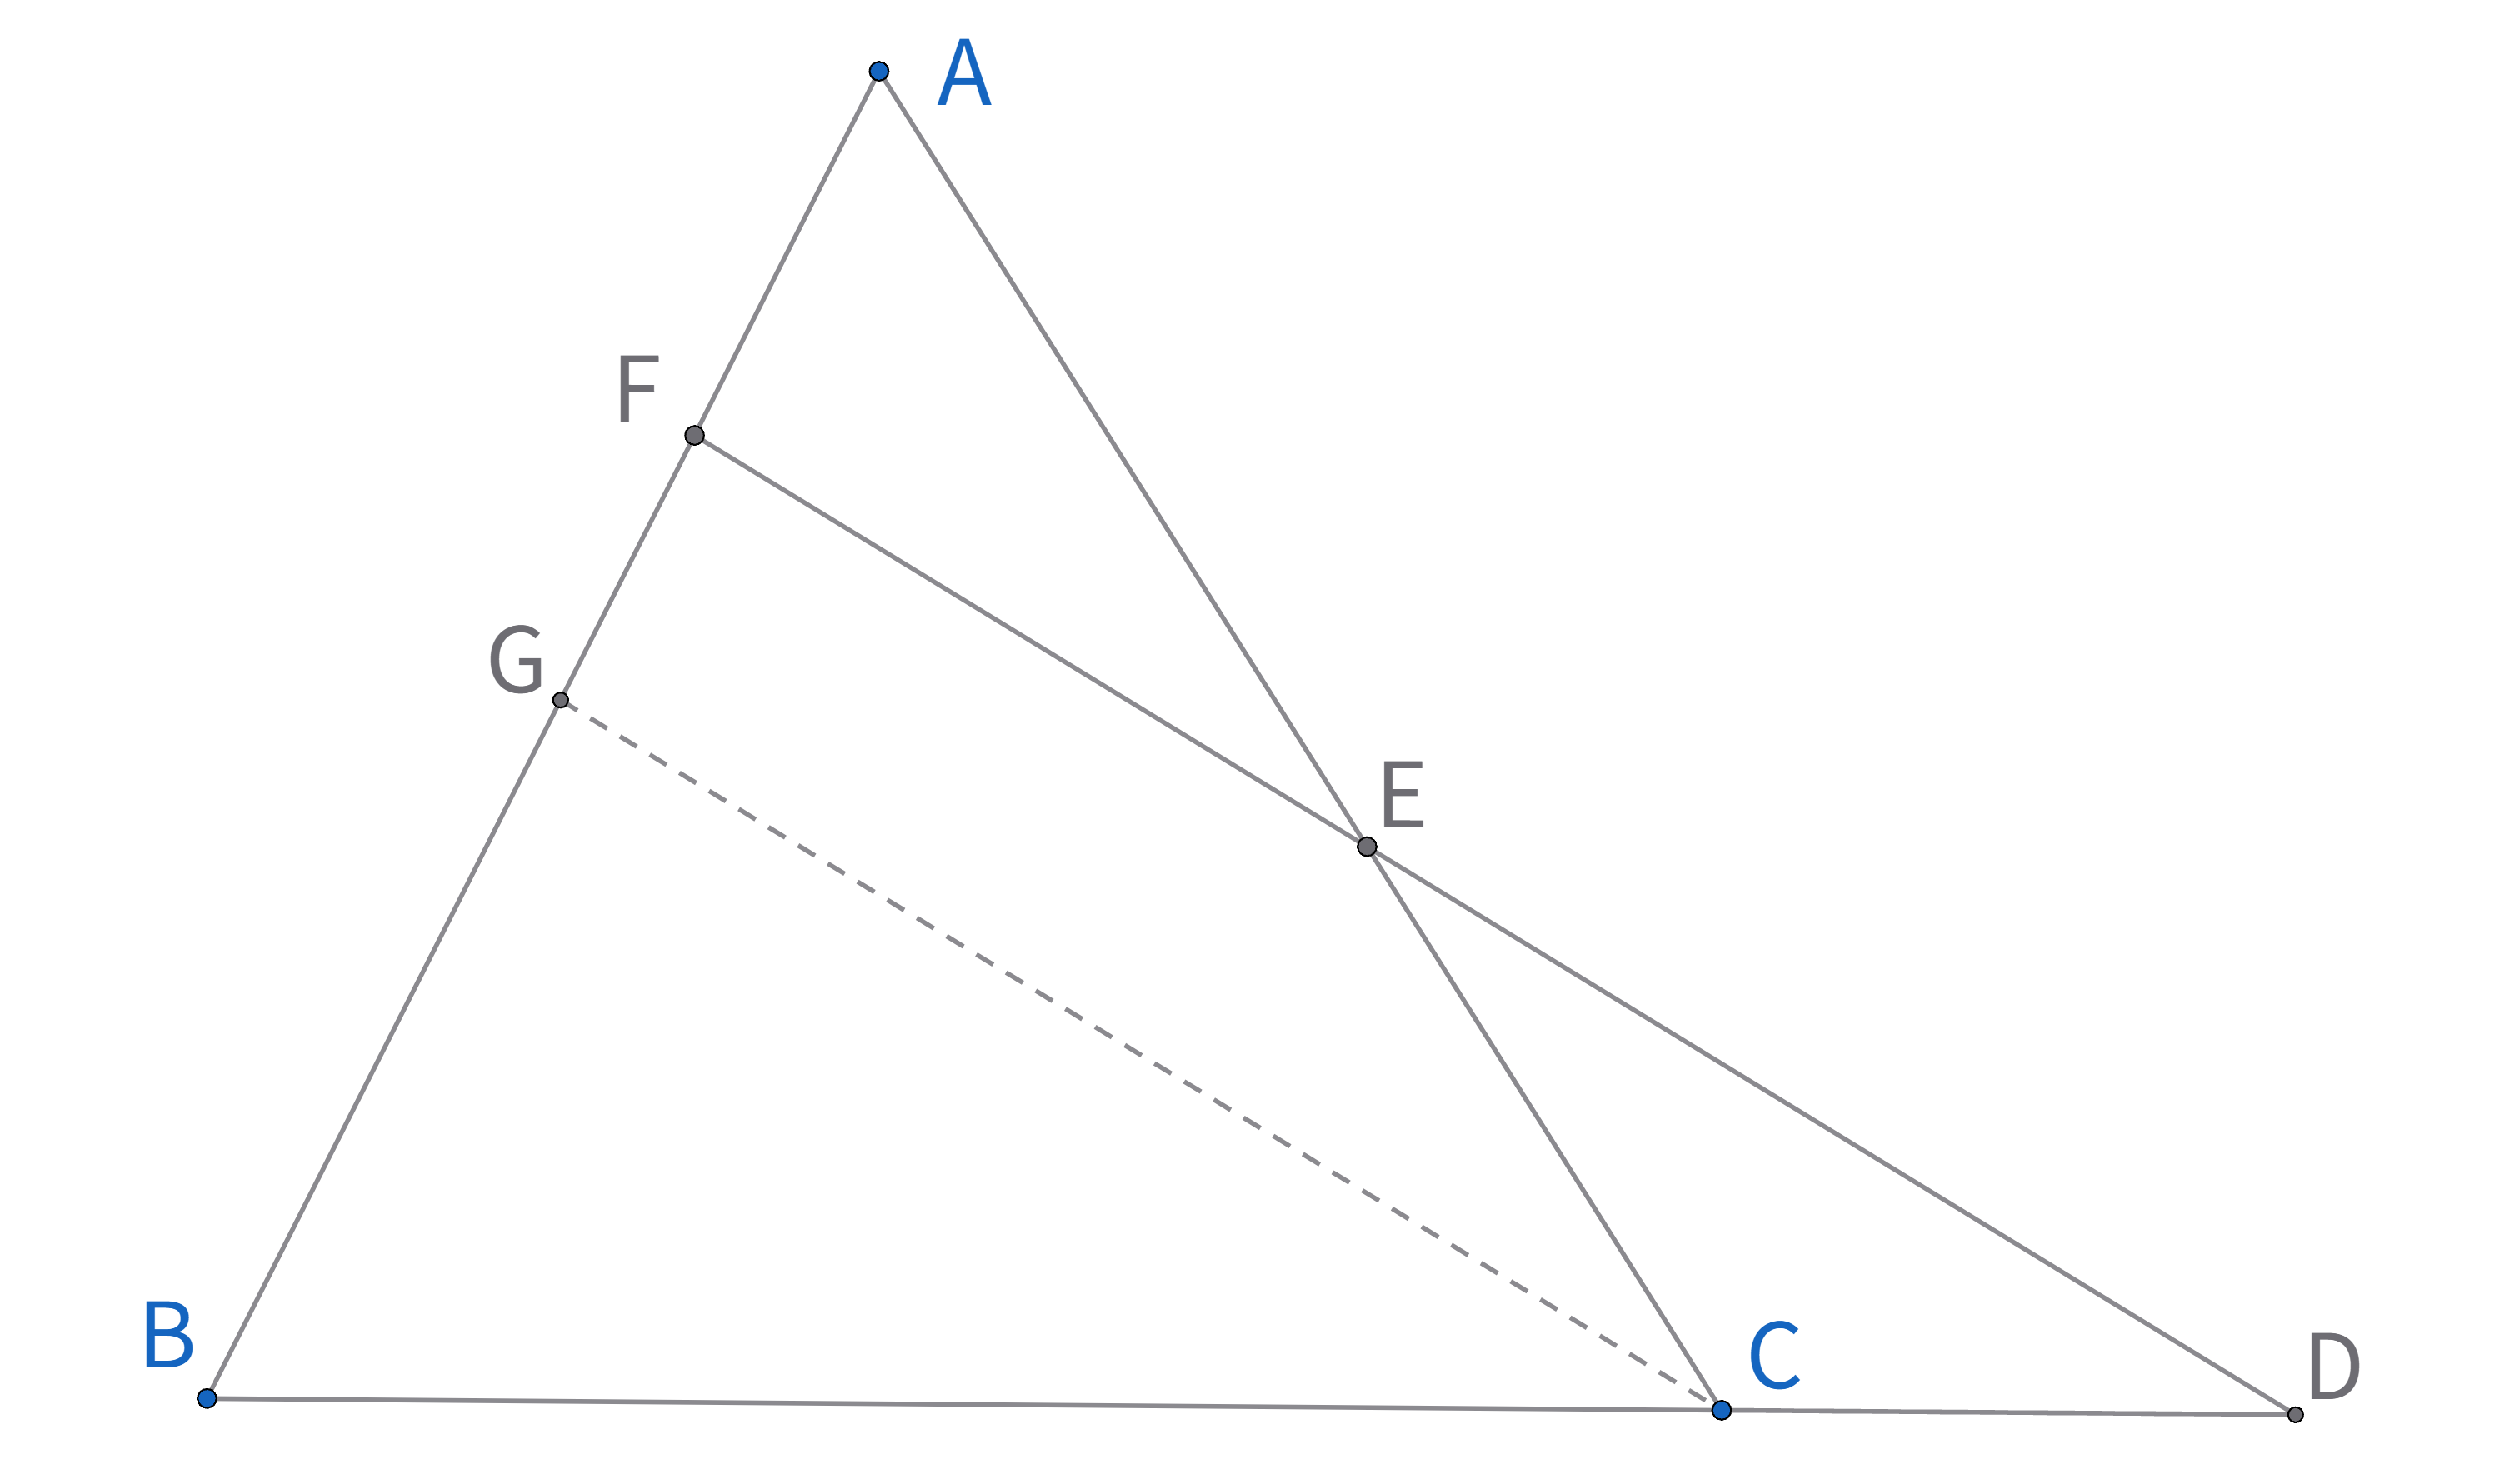
\includegraphics[width=\linewidth]{figures/menelaus-proof1.png}
    \end{minipage}
    \hfill % 添加一些水平间距
    \begin{minipage}[t]{0.45\textwidth}
    \centering
    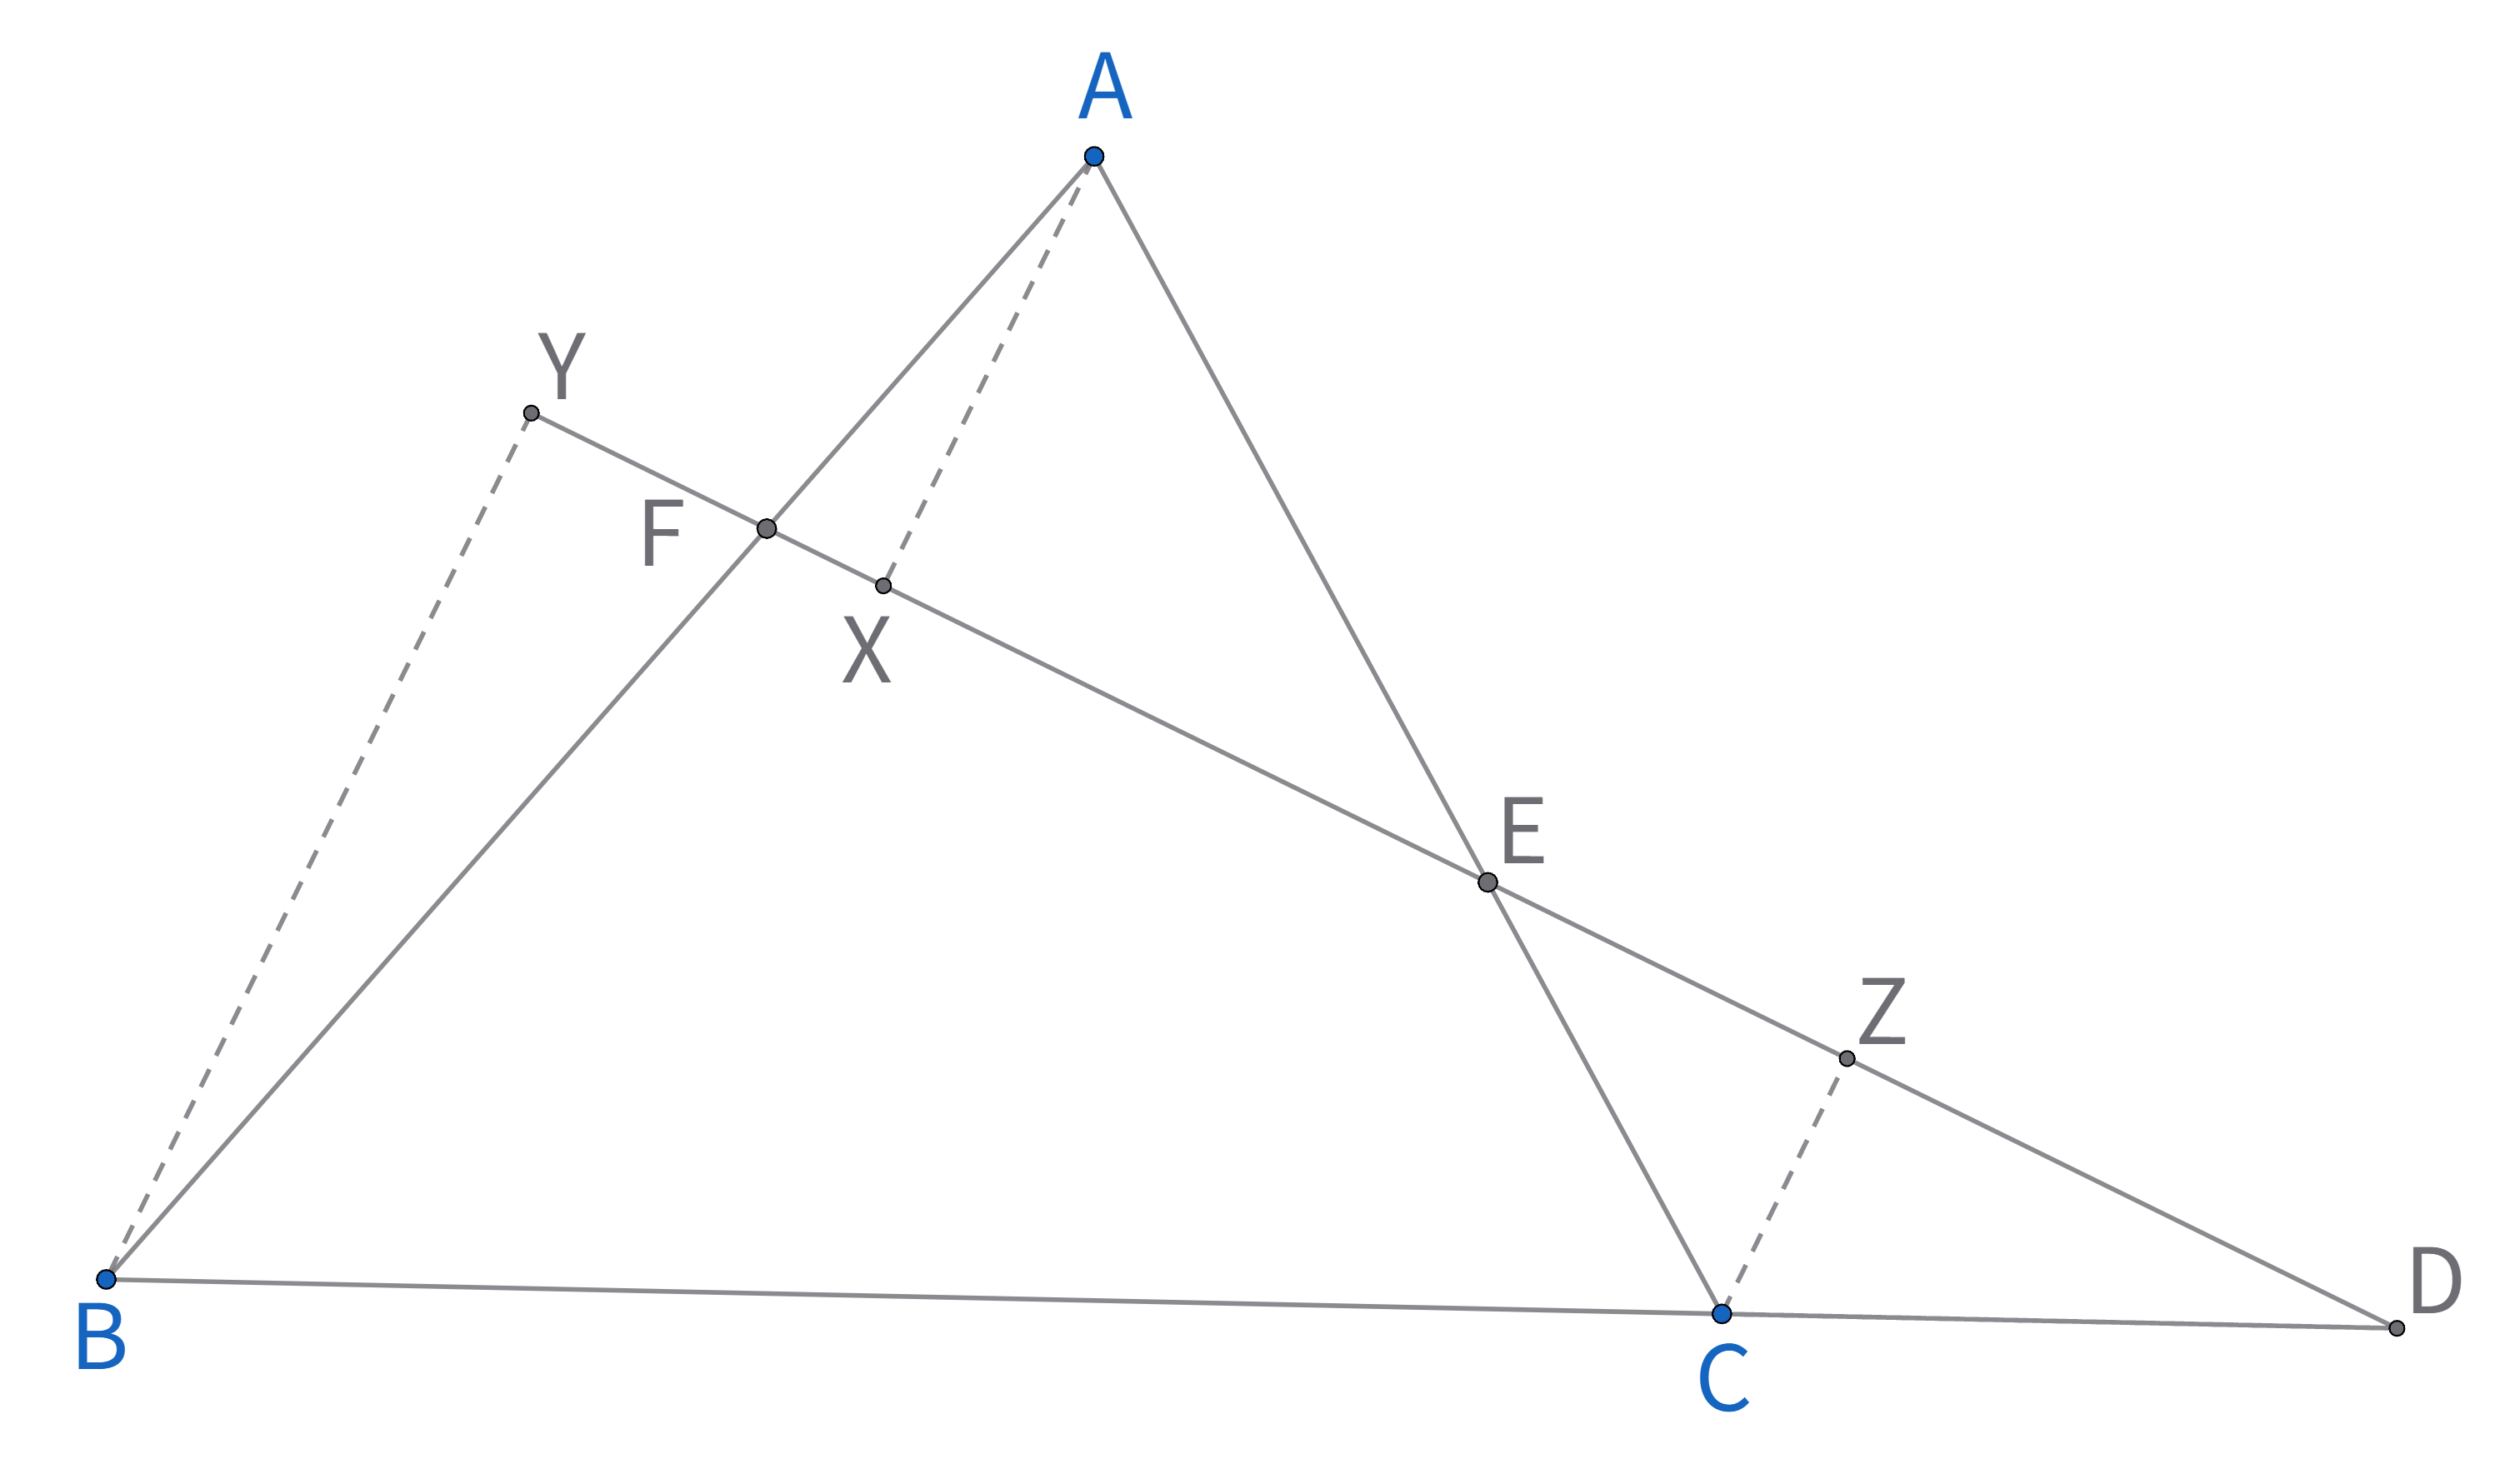
\includegraphics[width=\linewidth]{figures/menelaus-proof2.png}
    \end{minipage}
\end{figure}

\begin{remark}
    梅涅劳斯定理中的恒等式可以按照顶点-截点-顶点的顺序记忆。
    
    例如对$\triangle ABC$首先确定三边顺序AB、BC、AC,然后确定各个边上的截点X、Y、Z,与各边顶点连接起来就得到了(AX-XB)-(BY-YC)-(CZ-ZA)。

    截线XYZ可以交于三边的延长线。

    正定理多用于获得截线段比值关系,逆定理多用于证明三点共线问题。
\end{remark}


%---------------------------------------------------
\section{塞瓦定理}
\begin{theorem}[塞瓦(Ceva)定理]
    已知平面上 $\triangle A B C$ 和点 $P$( $P$ 不在 $\triangle A B C$ 三边上),直线 $A P 、 B P 、 C P$ 分别与直线 $B C 、 C A 、 A B$ 交于点 $X 、 Y 、 Z$ ,则 
    $$\frac{A Z}{Z B} \cdot \frac{B X}{X C} \cdot \frac{C Y}{Y A}=1.$$
\end{theorem}


\begin{figure}[H]
    \centering
    % \hfill % 添加一些水平间距
    \begin{minipage}[t]{0.2\textwidth}
    \centering
    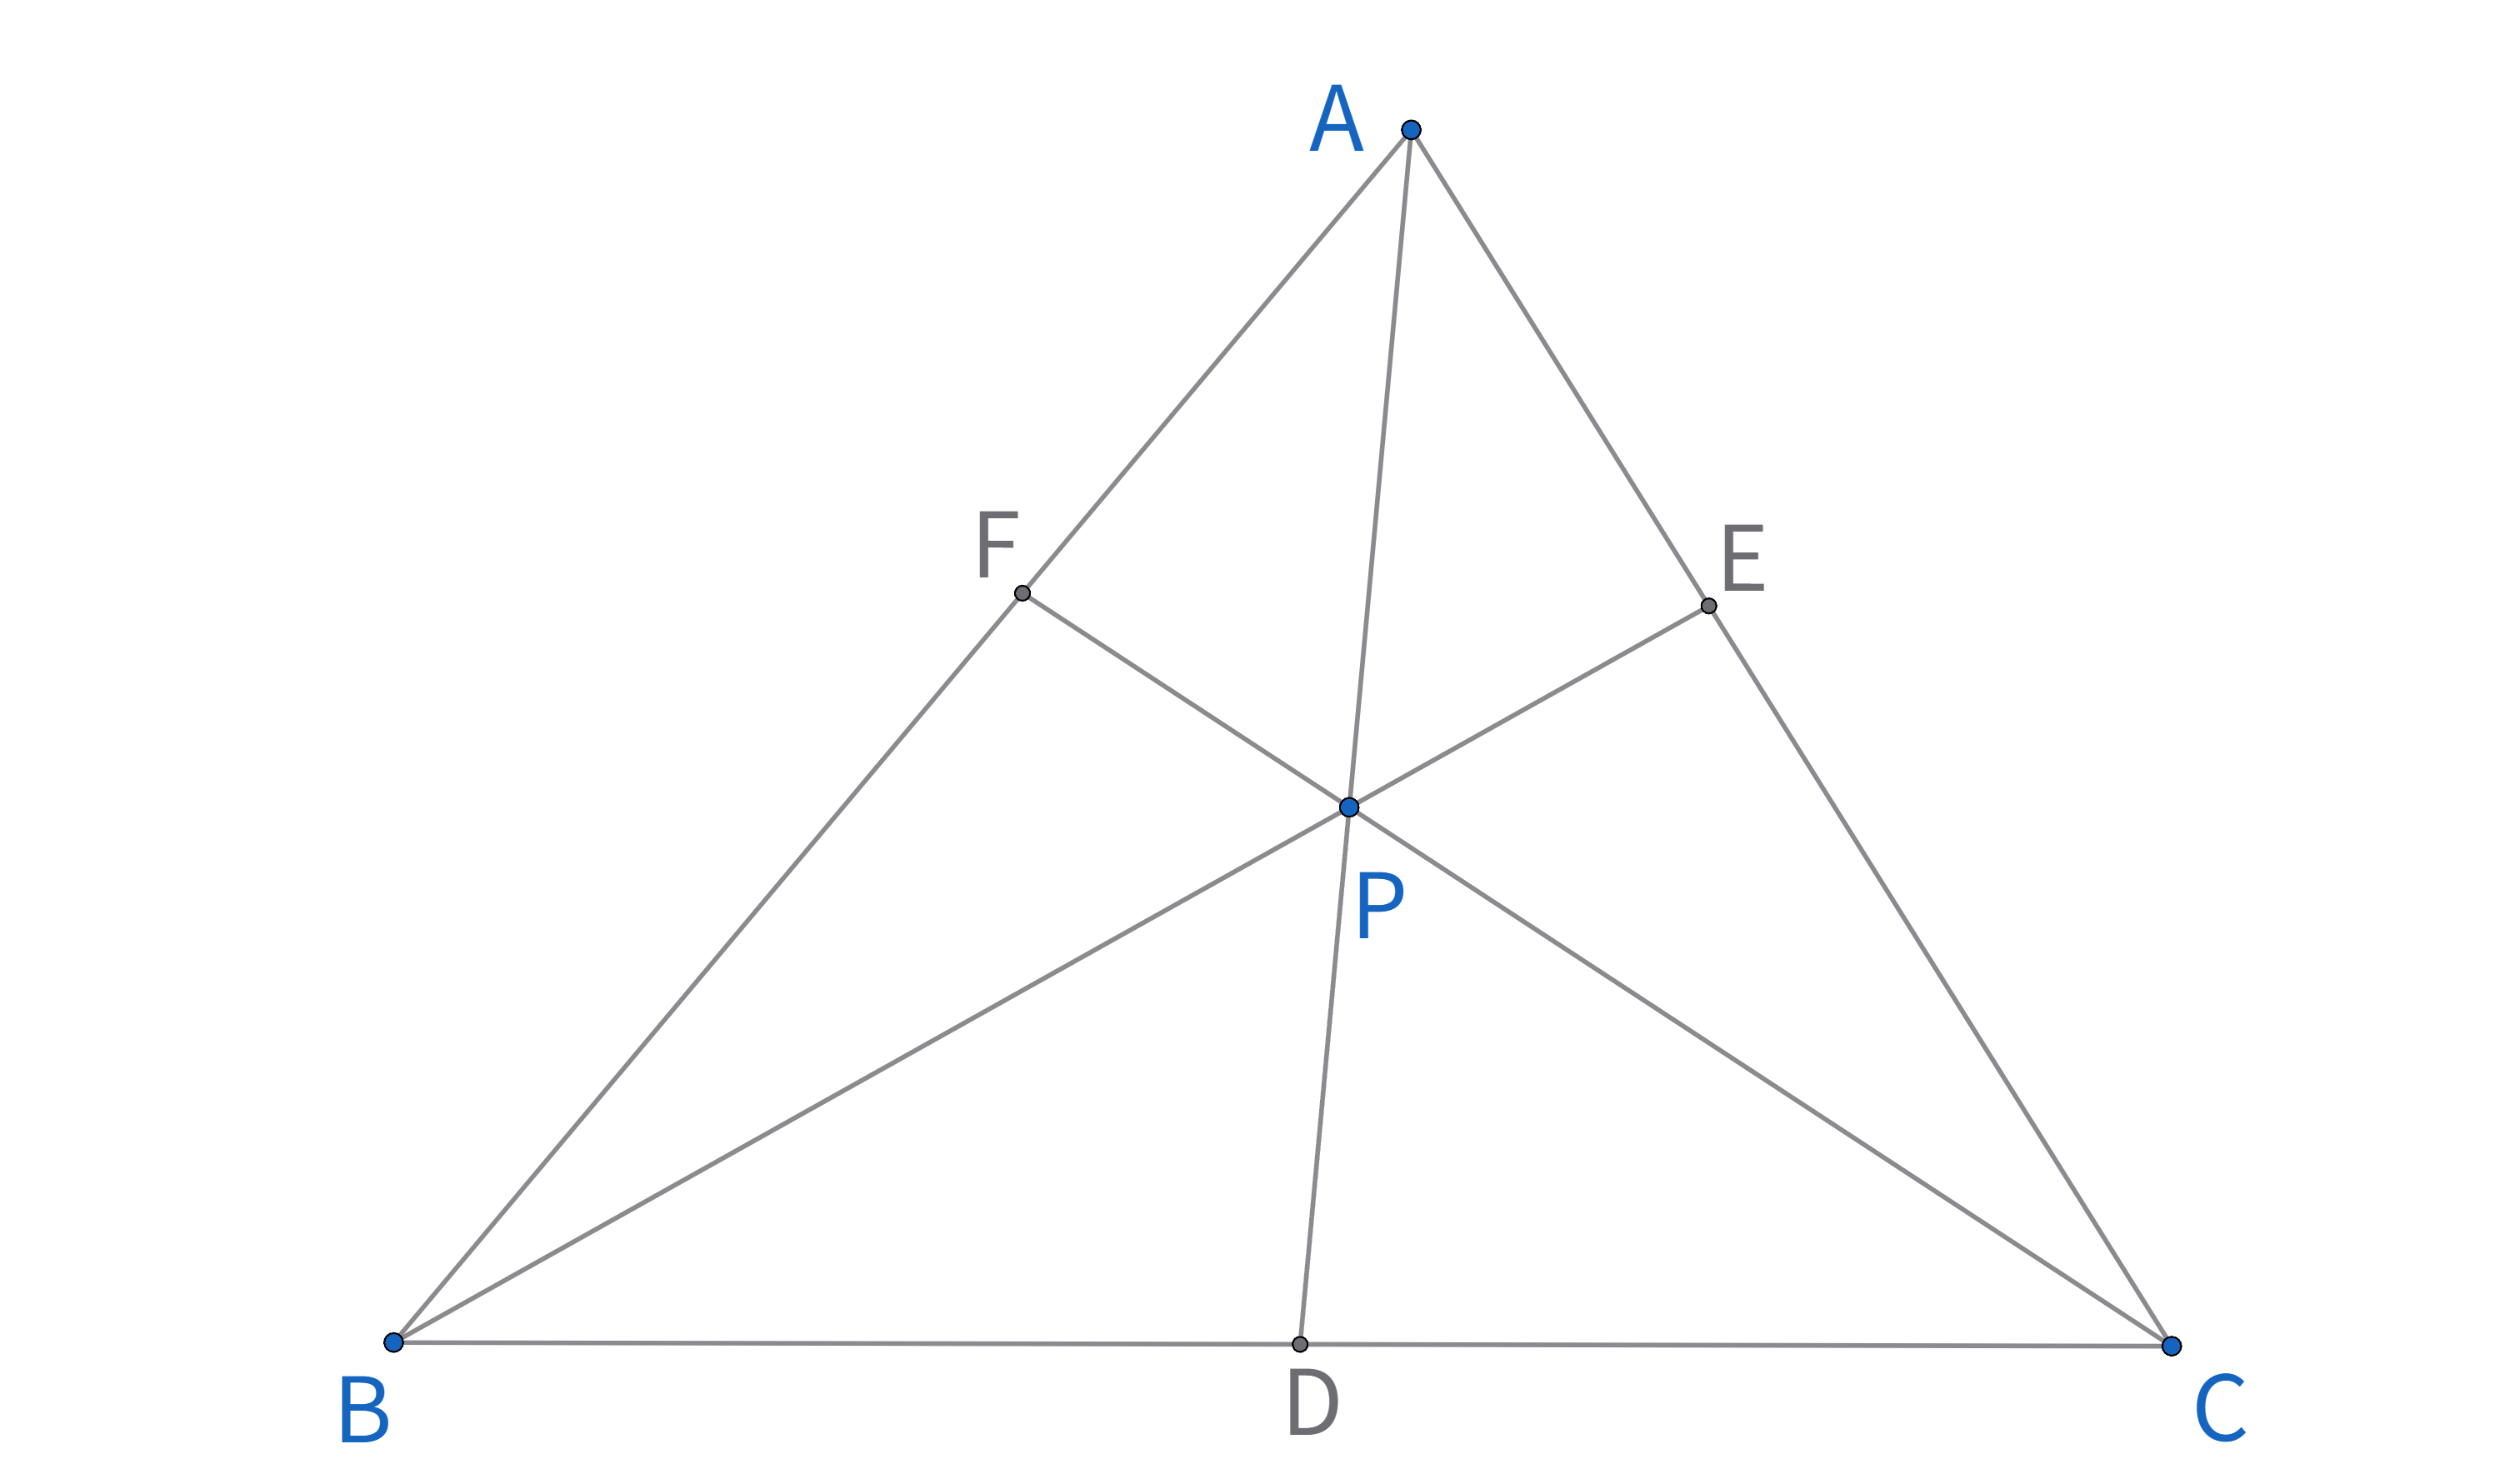
\includegraphics[width=\linewidth]{figures/ceva1.png}
    \end{minipage}
    % \hfill % 添加一些水平间距
    \begin{minipage}[t]{0.2\textwidth}
    \centering
    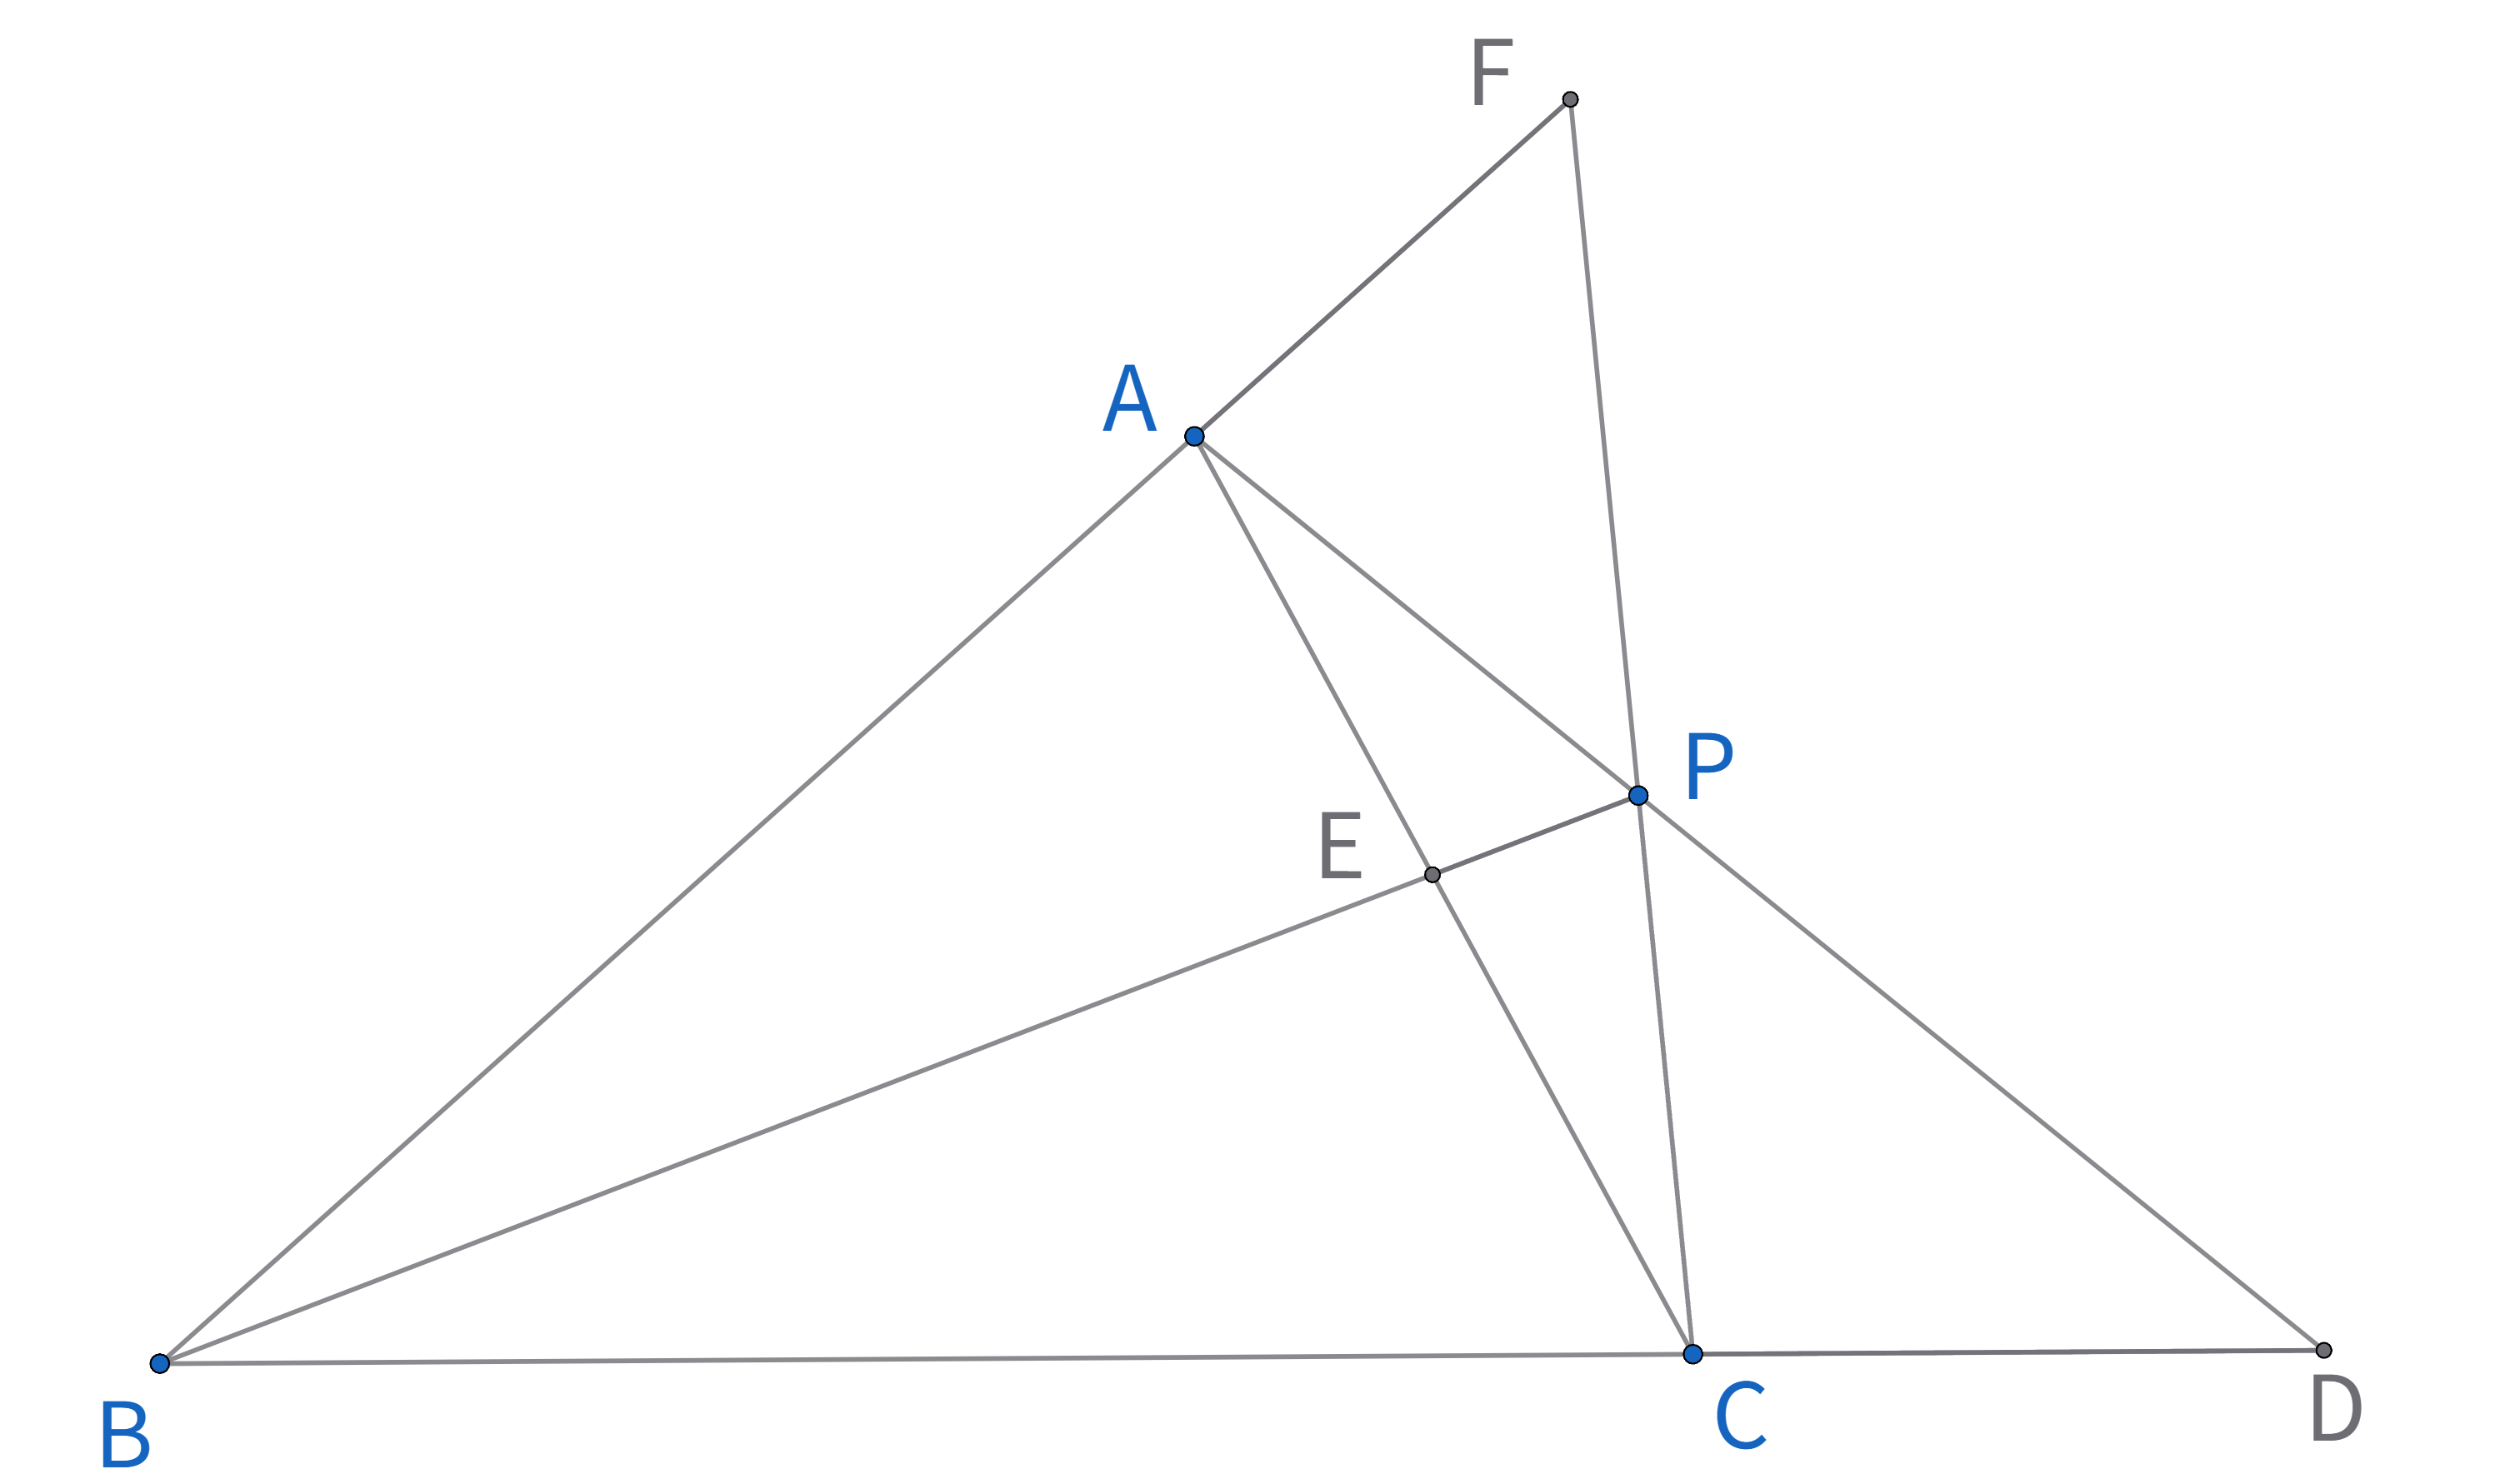
\includegraphics[width=\linewidth]{figures/ceva2.png}
    \end{minipage}
    % \hfill % 添加一些水平间距
    \begin{minipage}[t]{0.2\textwidth}
    \centering
    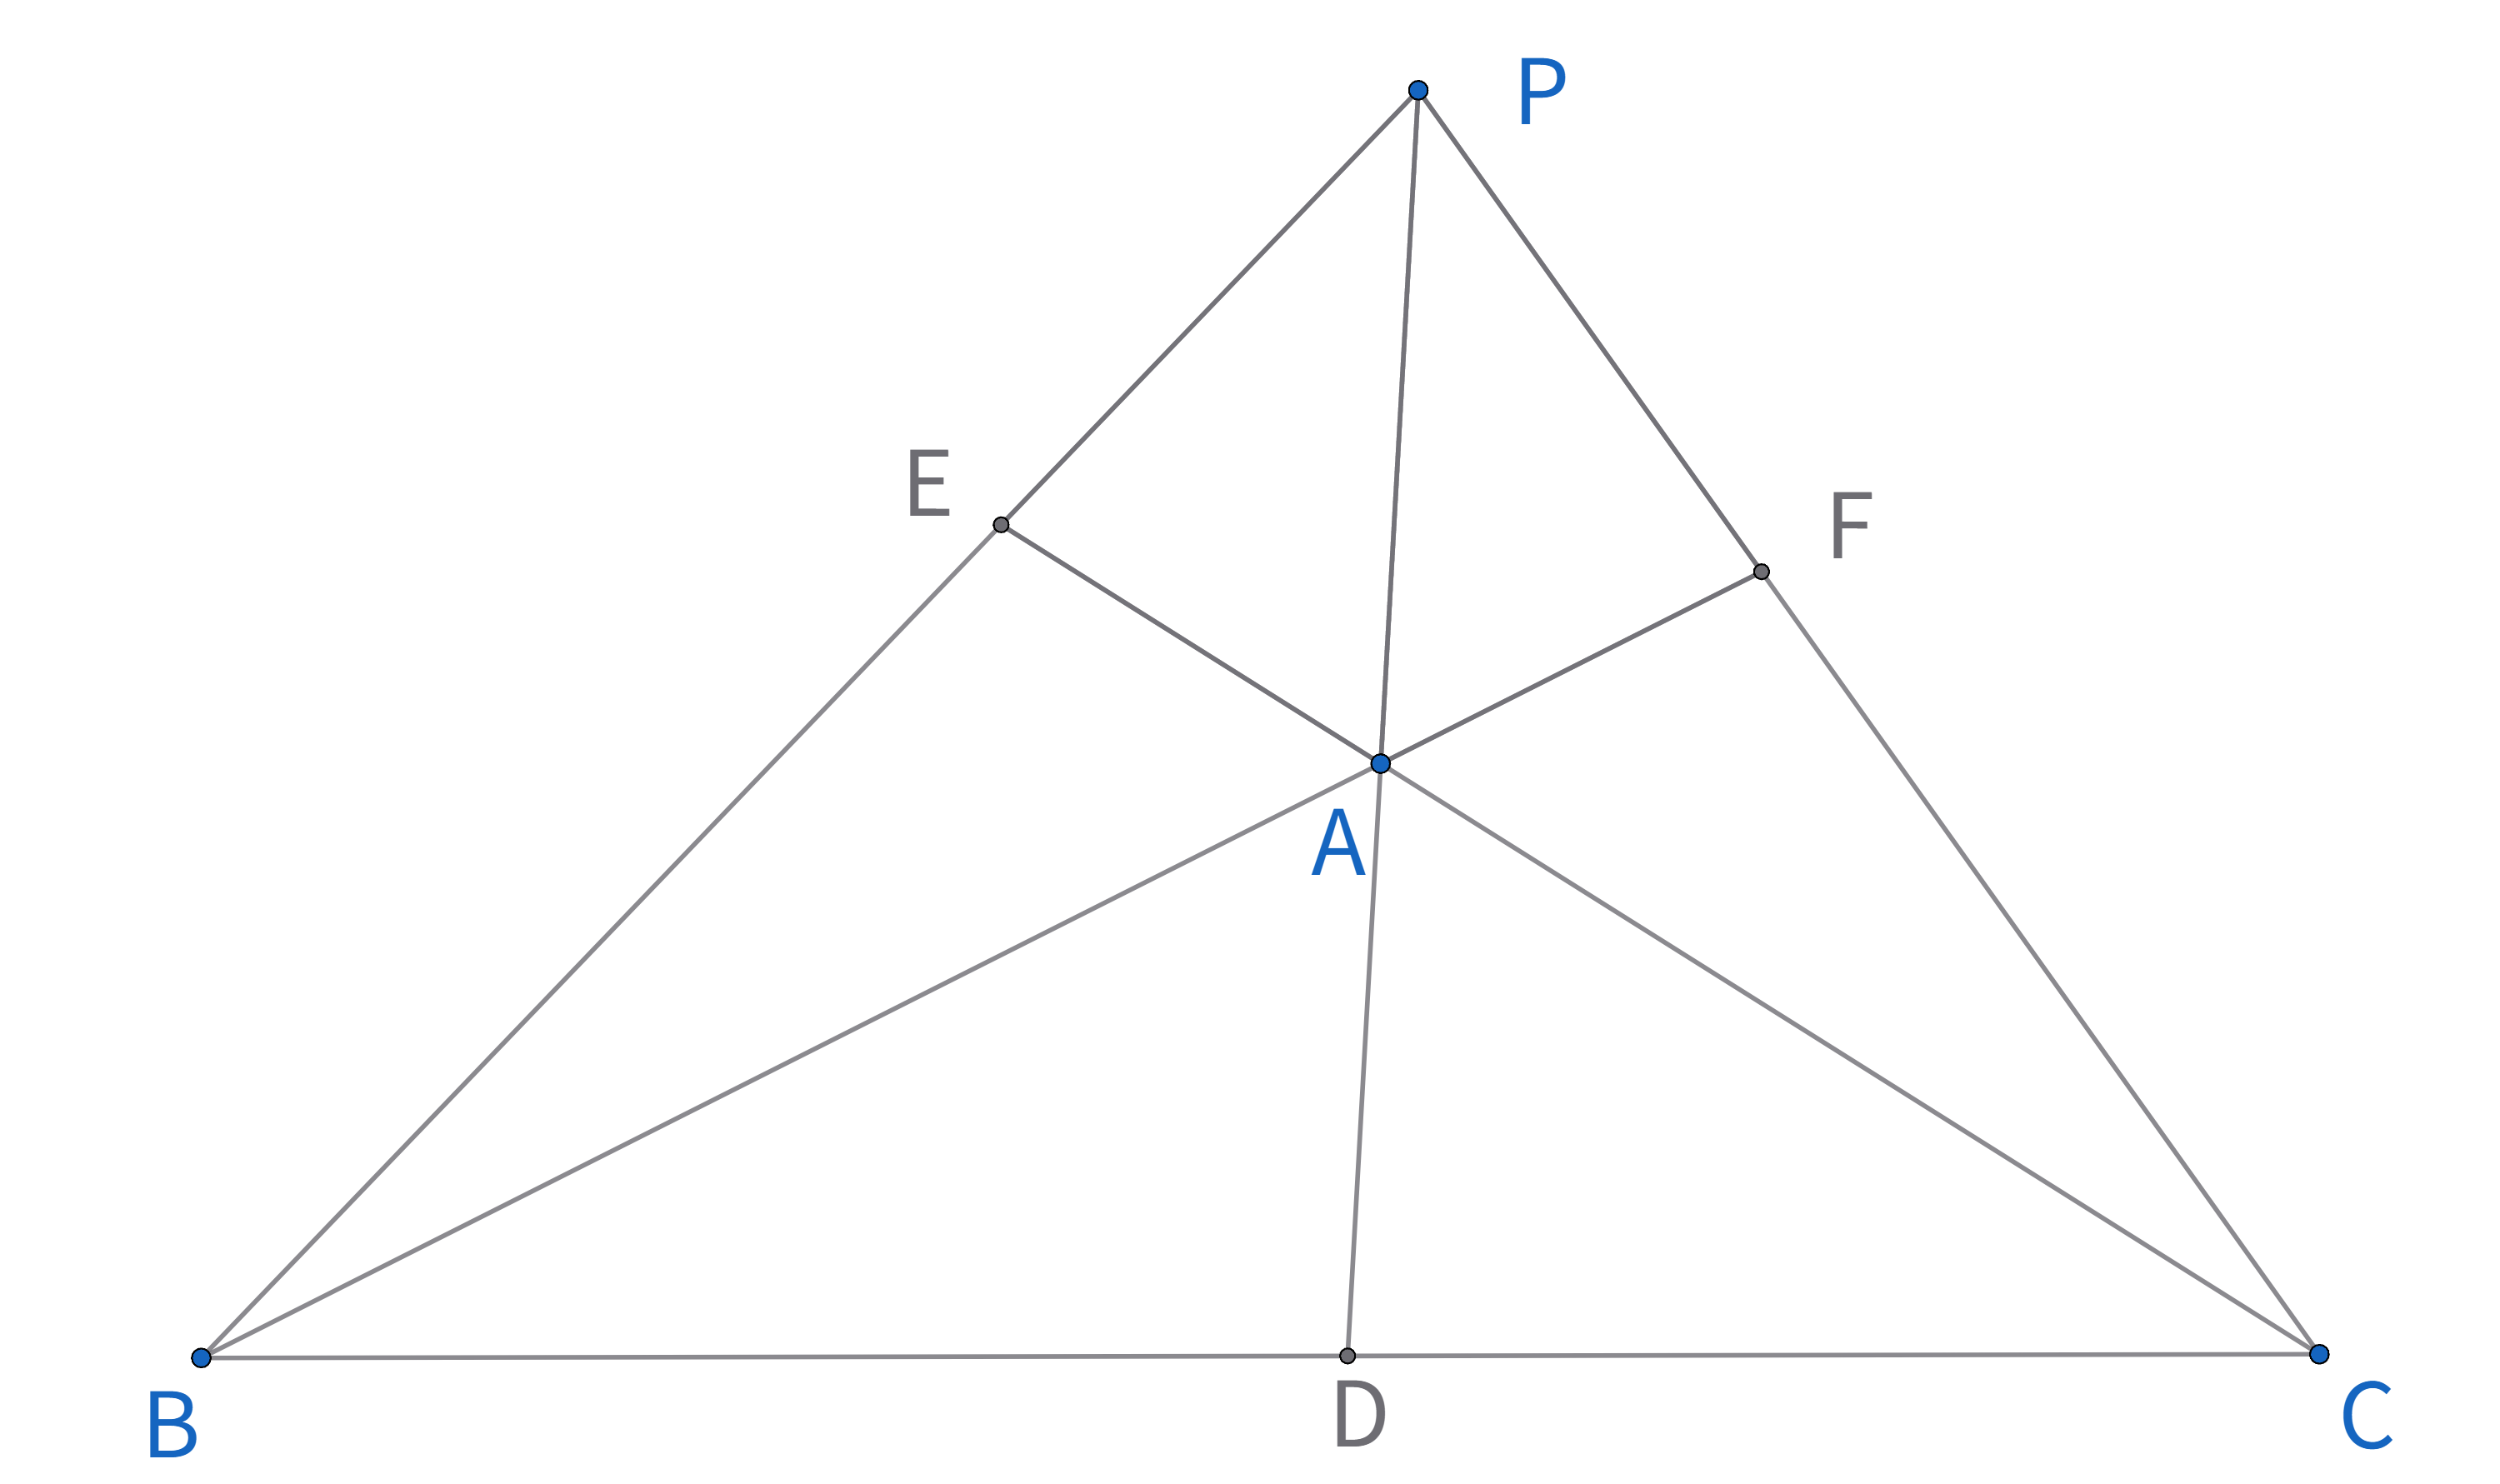
\includegraphics[width=\linewidth]{figures/ceva3.png}
    \end{minipage}
    % \hfill % 添加一些水平间距
    \begin{minipage}[t]{0.2\textwidth}
    \centering
    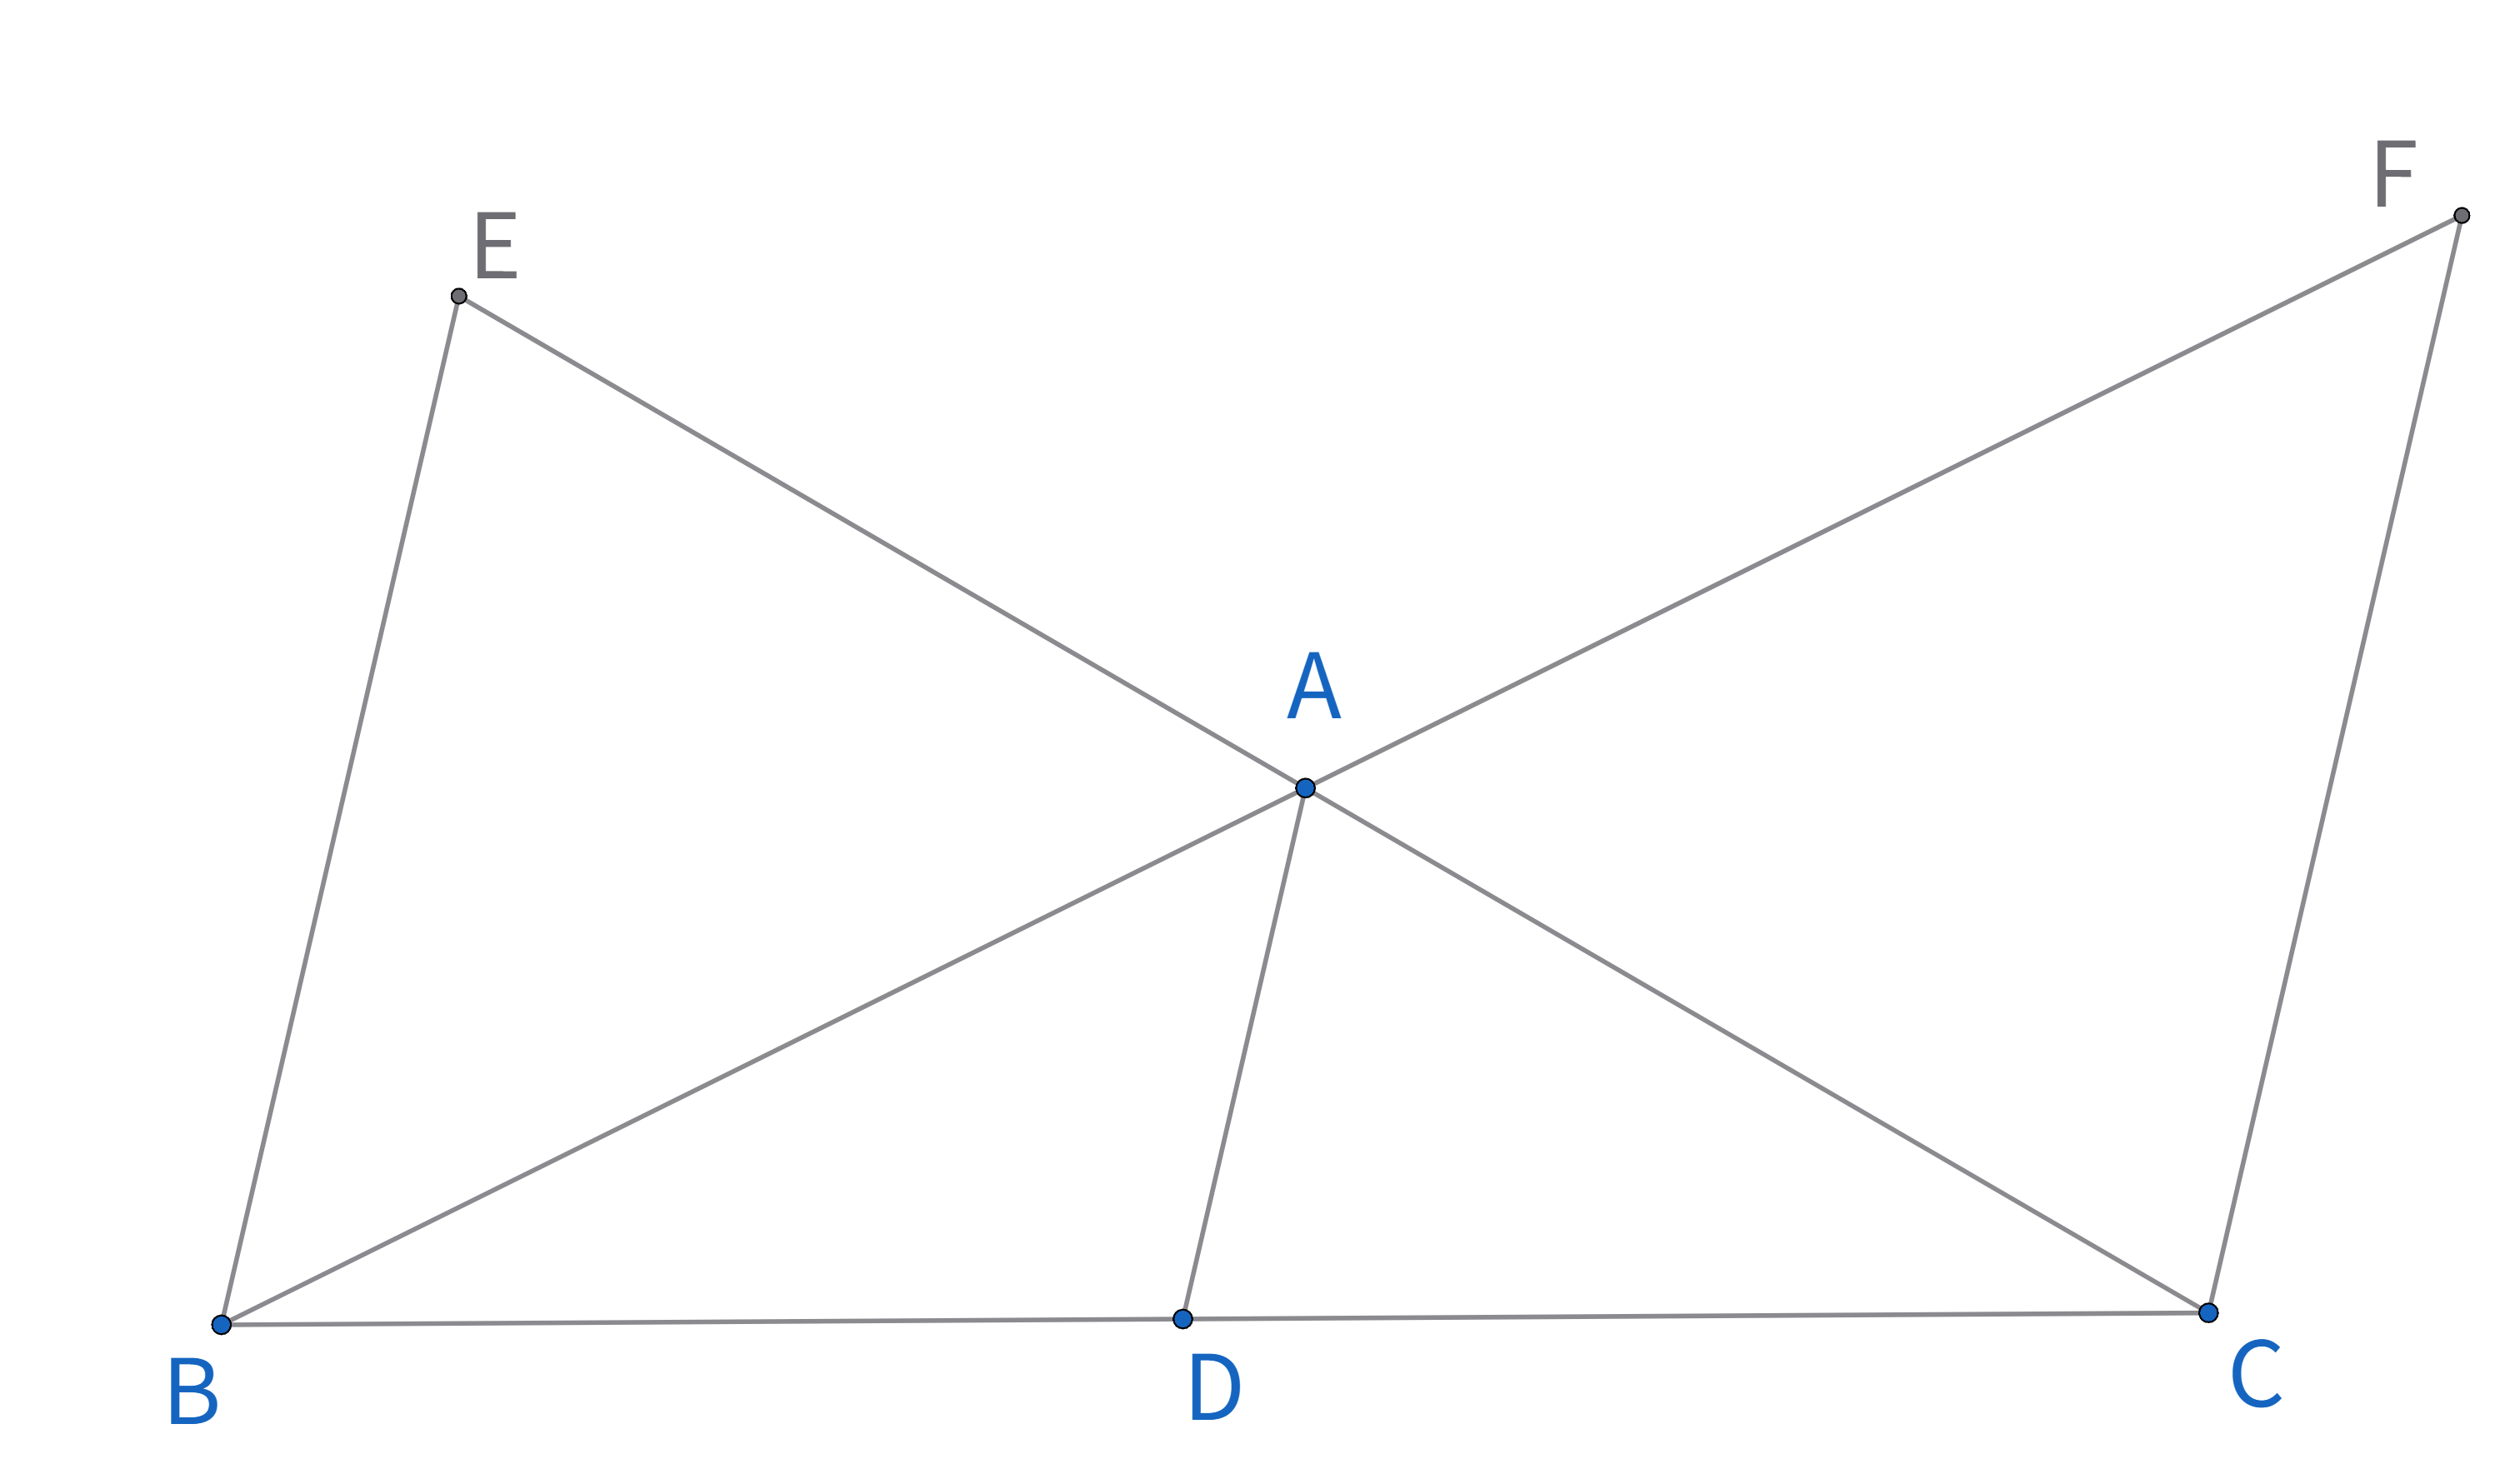
\includegraphics[width=\linewidth]{figures/ceva4.png}
    \end{minipage}
    \caption{四种情形的塞瓦定理}
\end{figure}


\begin{theorem}[塞瓦(Ceva)逆定理]
如果 $X 、 Y 、 Z$ 中有奇数个点在 $\triangle A B C$ 的三边上,且点 $X 、 Y 、$ $Z$ 分别为 $\triangle A B C$ 的三边 $B C 、 C A 、 A B$ 所在直线上的点,满足 
$$\frac{A Z}{Z B} \cdot \frac{B X}{X C} \cdot \frac{C Y}{Y A}=1,$$
则 $A X 、 B Y 、 C Z$ 三条直线交于一点或彼此平行.
\end{theorem}


\begin{figure}[H]
    \centering
    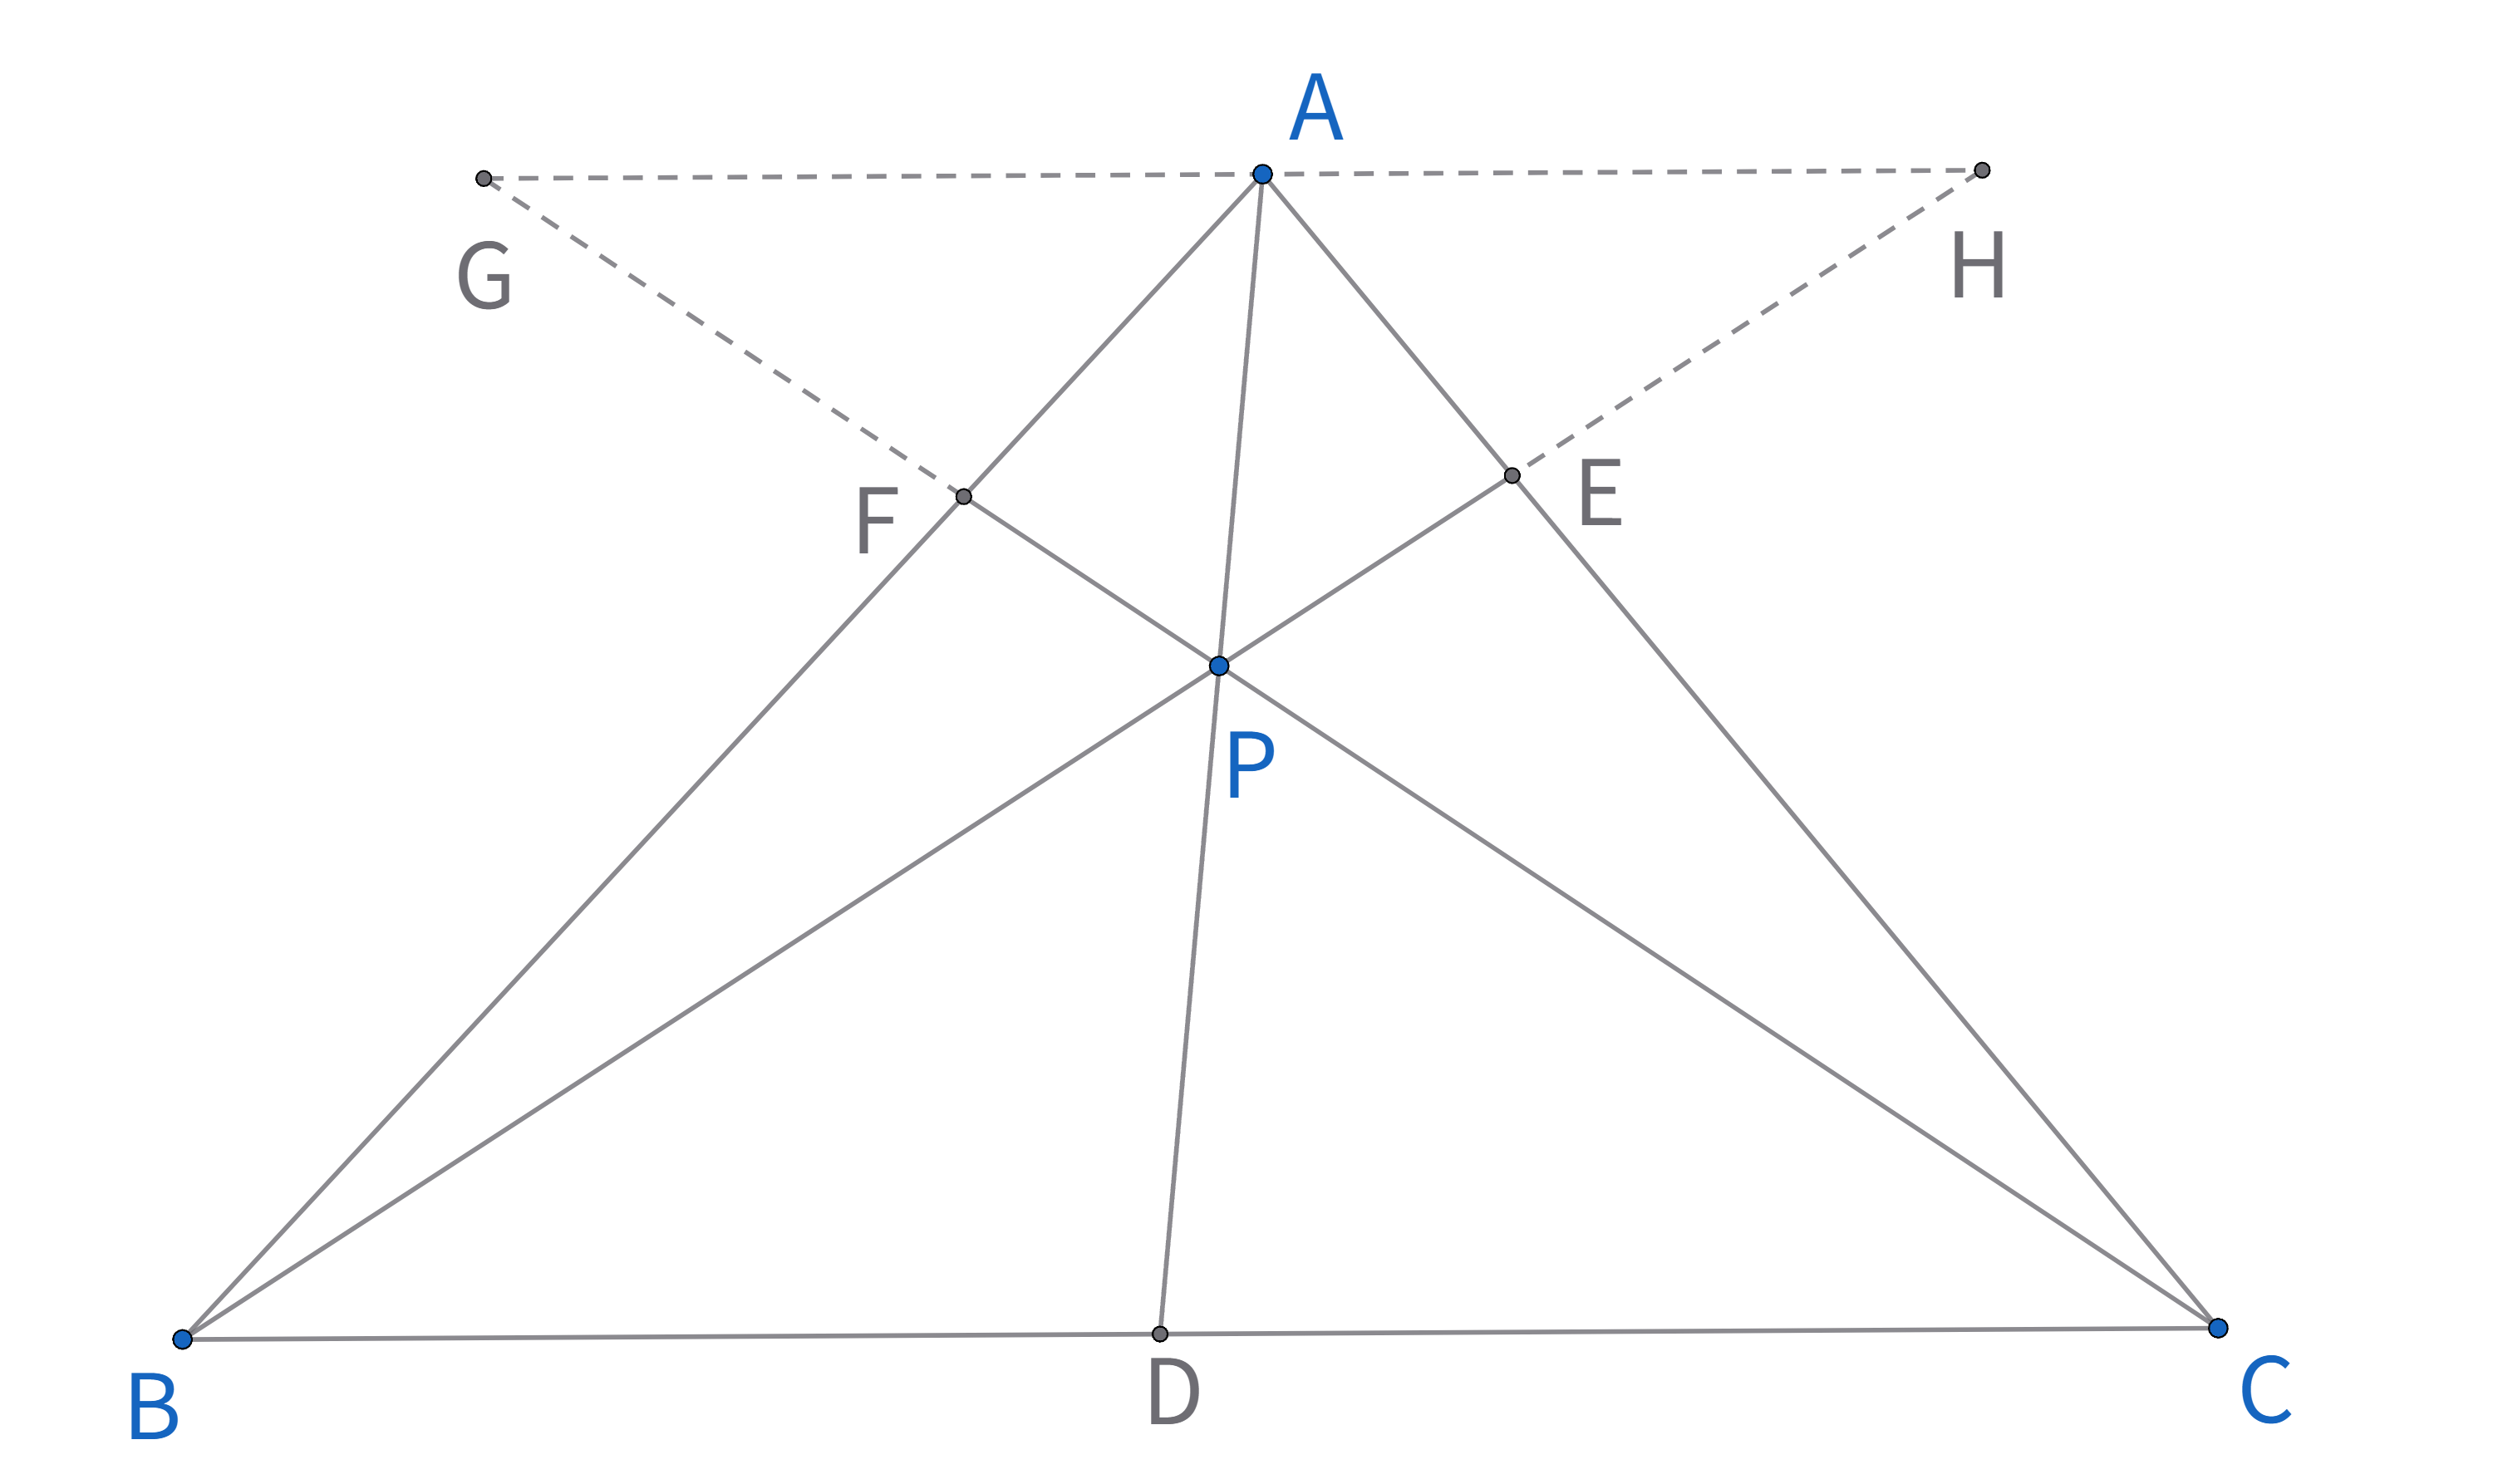
\includegraphics[width=0.6\linewidth]{figures/ceva-proof1.png}
\end{figure}
\begin{remark}
    塞瓦定理与梅涅劳斯定理的记忆方法类似,都是按照顶点-截点-顶点的顺序。

    塞瓦定理中点P可以不在$\triangle ABC$形内。
    
    P为无穷原点时,BE、AD、CF三线平行,等式依然成立。

    
\end{remark}


\begin{theorem}[角元形式赛瓦定理]
    已知平面上 $\triangle A B C$ 和点P( P不在$\triangle A B C$ 三边上)。设D、E、F分别是BC、CA、AB所在直线上的点。则AD、BE、CF三线共点等价于
    $$
    \frac{\sin \angle ABE}{\sin \angle EBC}
    \cdot 
    \frac{\sin \angle BCF}{\sin \angle FCA}
    \cdot 
    \frac{\sin \angle CAD}{\sin \angle DAB}
    =1
    $$
\end{theorem}


%---------------------------------------------------
\newpage 
\section{西姆松定理}
\begin{theorem}[西姆松(Simson)定理]
过$\triangle ABC$外接圆O上异于三角形顶点的任意一点P作三边所在直线的垂线,则三垂足共线,此线称为西姆松线(Simson line)。

西姆松定理的逆定理为:若一点P在$\triangle ABC$三边所在直线上的射影共线,则该点在此三角形的外接圆上。
\end{theorem}

\begin{figure}[H]
    \centering
    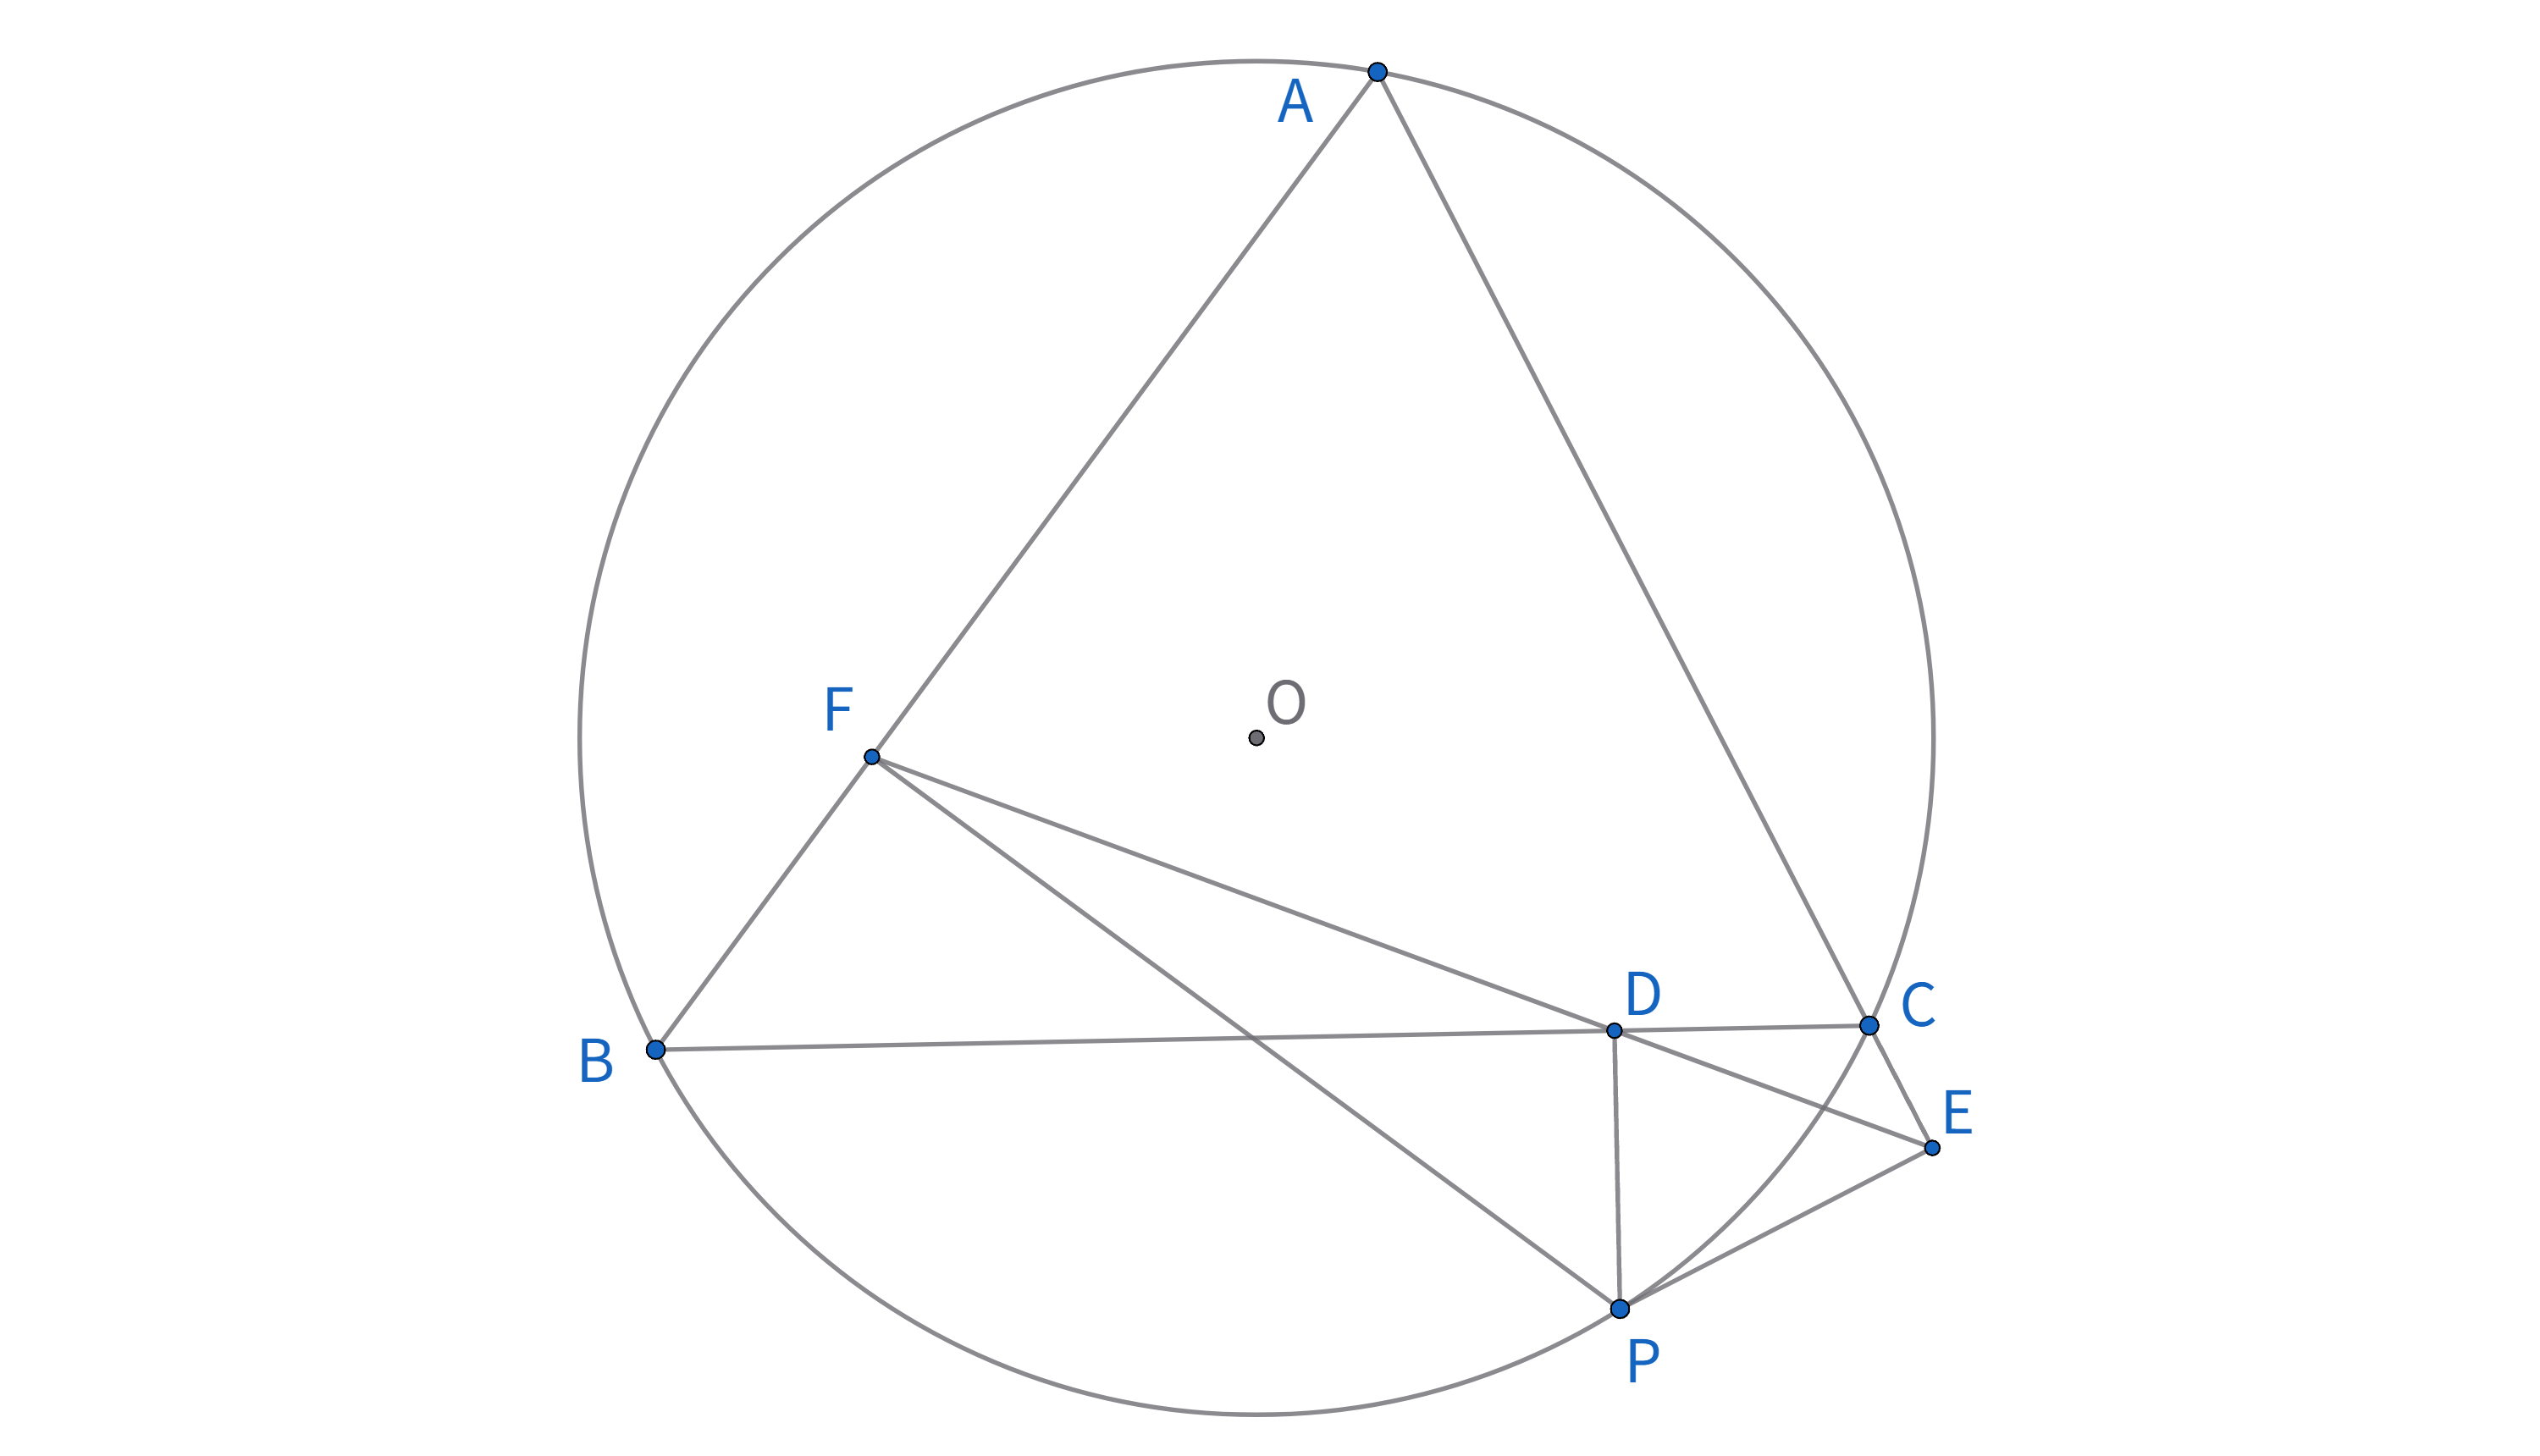
\includegraphics[width=\linewidth]{figures/西姆松线.png}
    \caption{西姆松线}
\end{figure}


%---------------------------------------------------
\newpage
\section{帕普斯定理}
\begin{theorem}[帕普斯(Pappus)定理]
直线l1上依次有点A、B、C,直线l2上依次有点D、E、F。
设AE、BD交于P,AF、DC交于Q,BF、EC交于R,则P、Q、R共线。
\end{theorem}
\begin{figure}[H]
    \centering
    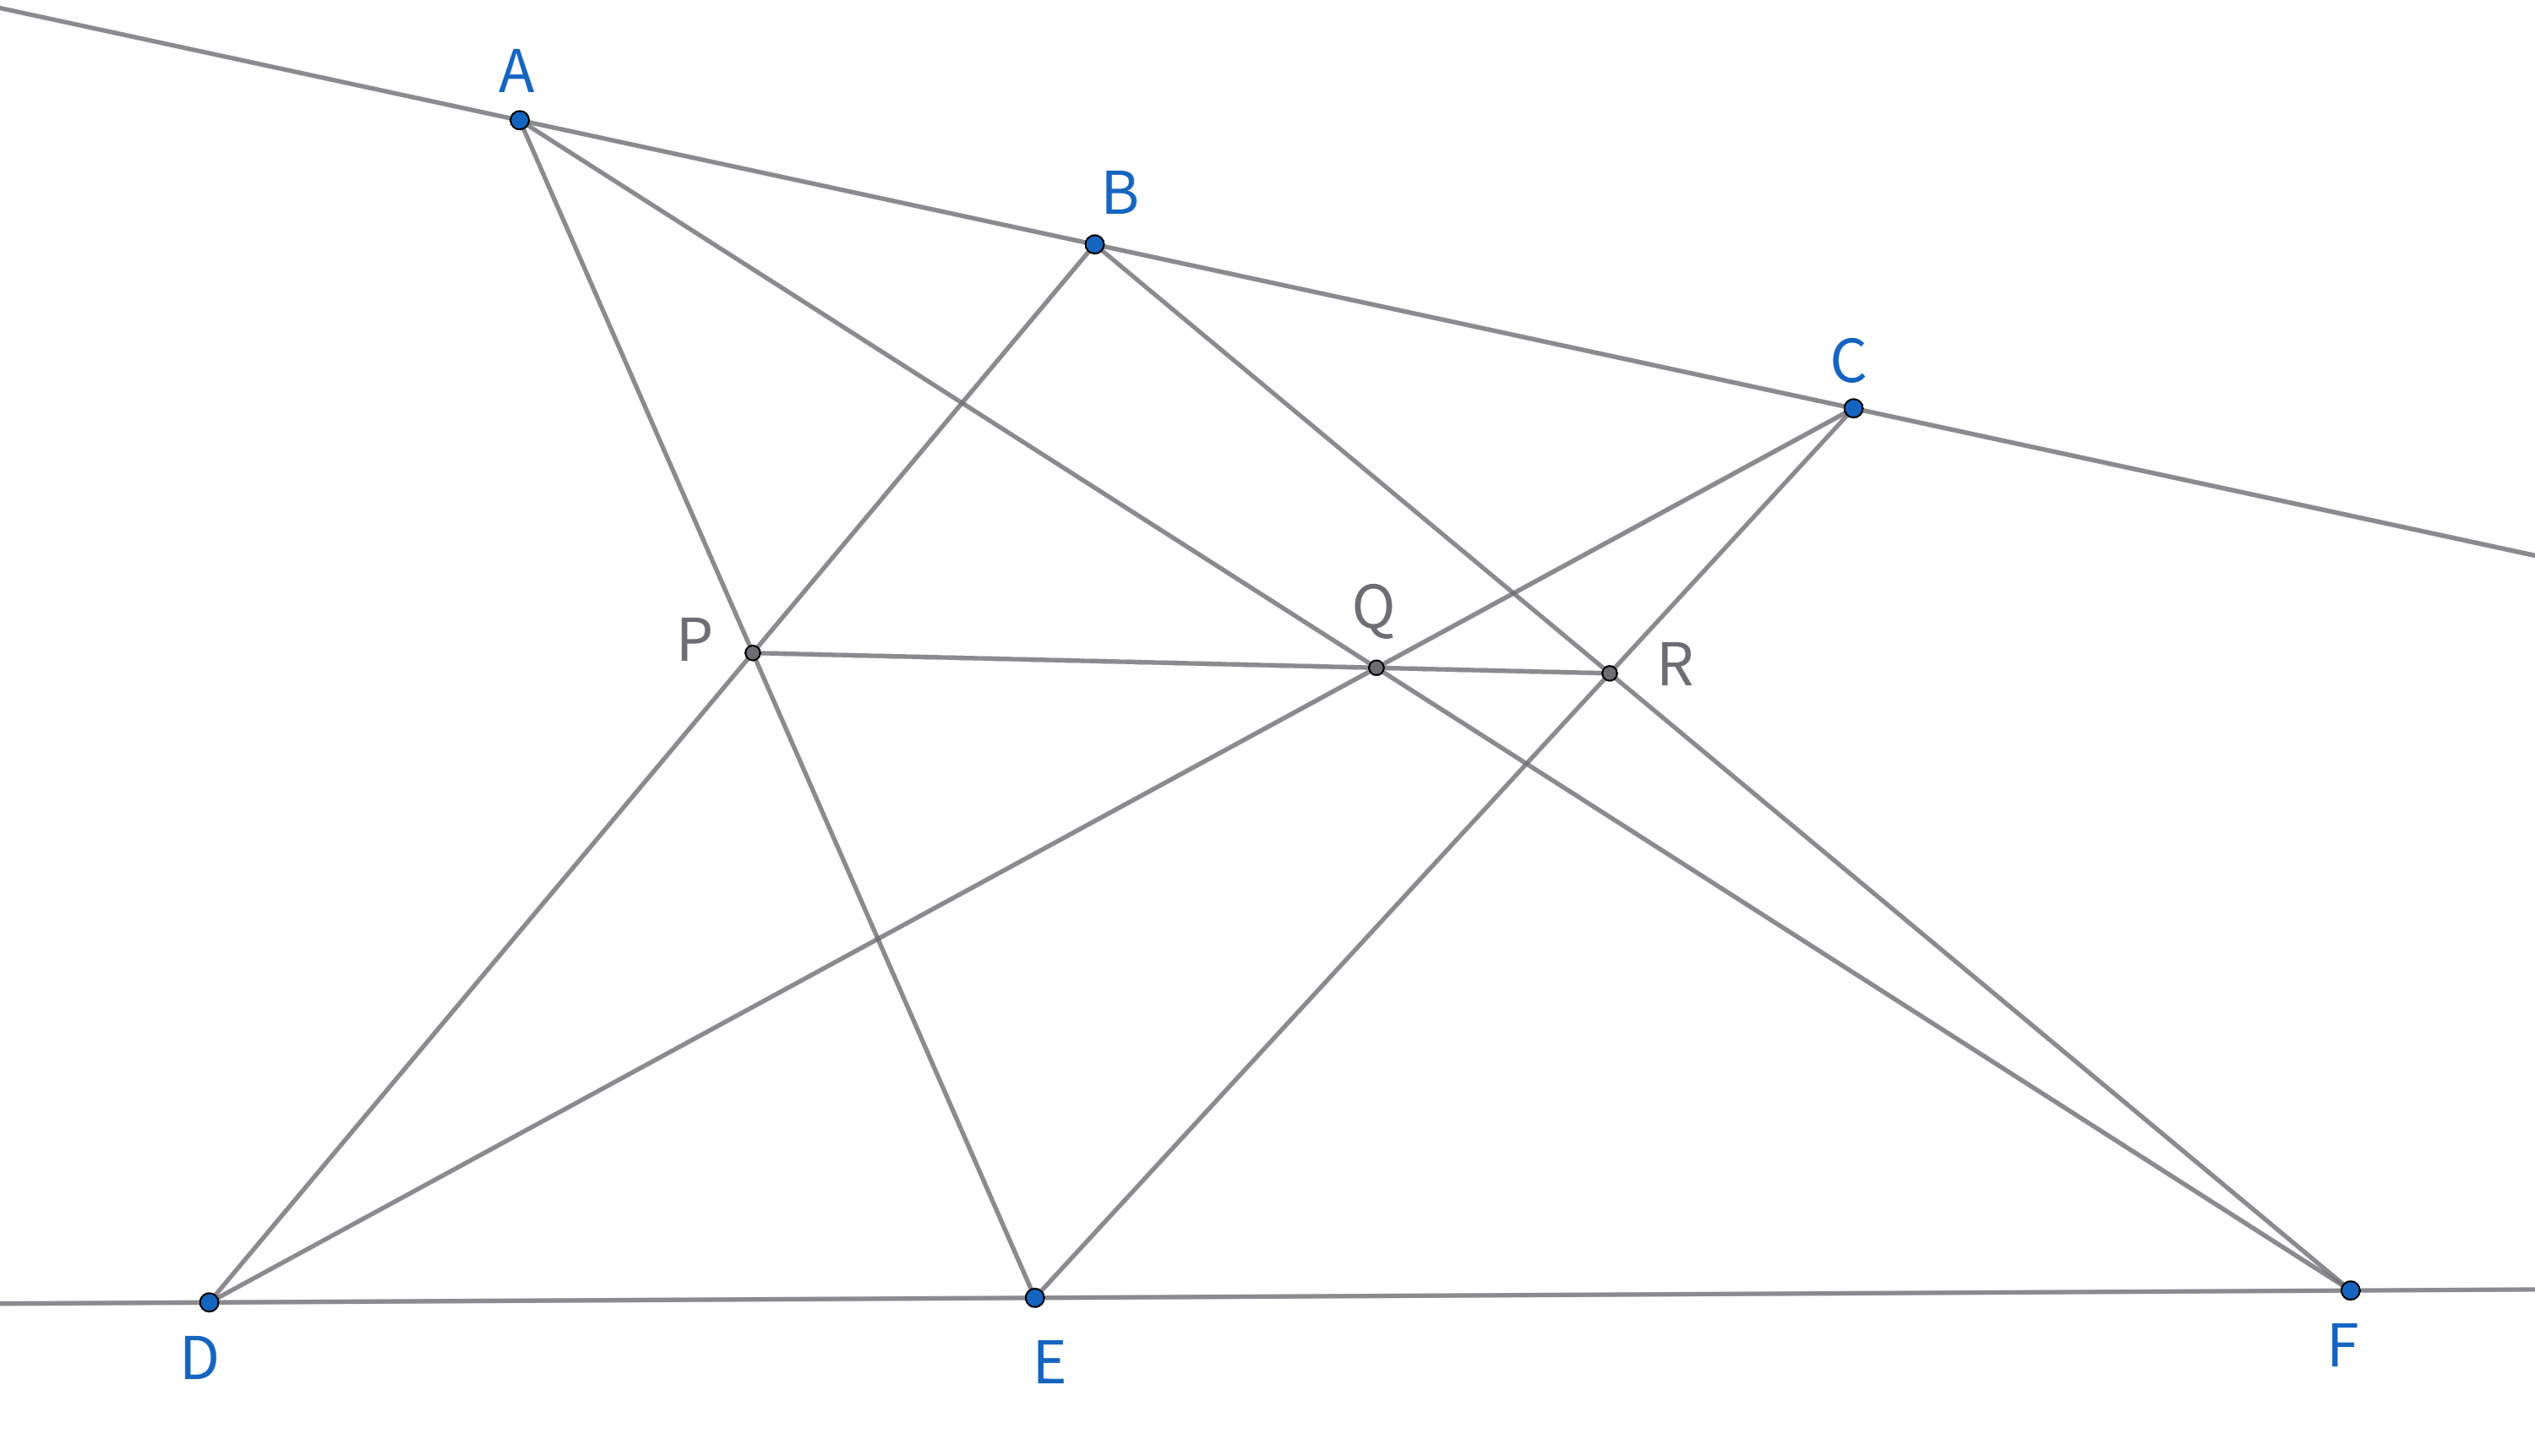
\includegraphics[width=\linewidth]{figures/帕普斯定理.png}
    \caption{帕普斯定理}
\end{figure}


%---------------------------------------------------
\newpage
\section{帕斯卡定理}
\begin{theorem}[帕斯卡(Pascal)定理]
设A、B、C、D、E、F为圆O上的点,
设AE、BD交于P,AF、DC交于Q,BF、EC交于R,则P、Q、R共线。
\end{theorem}
\begin{figure}[H]
    \centering
    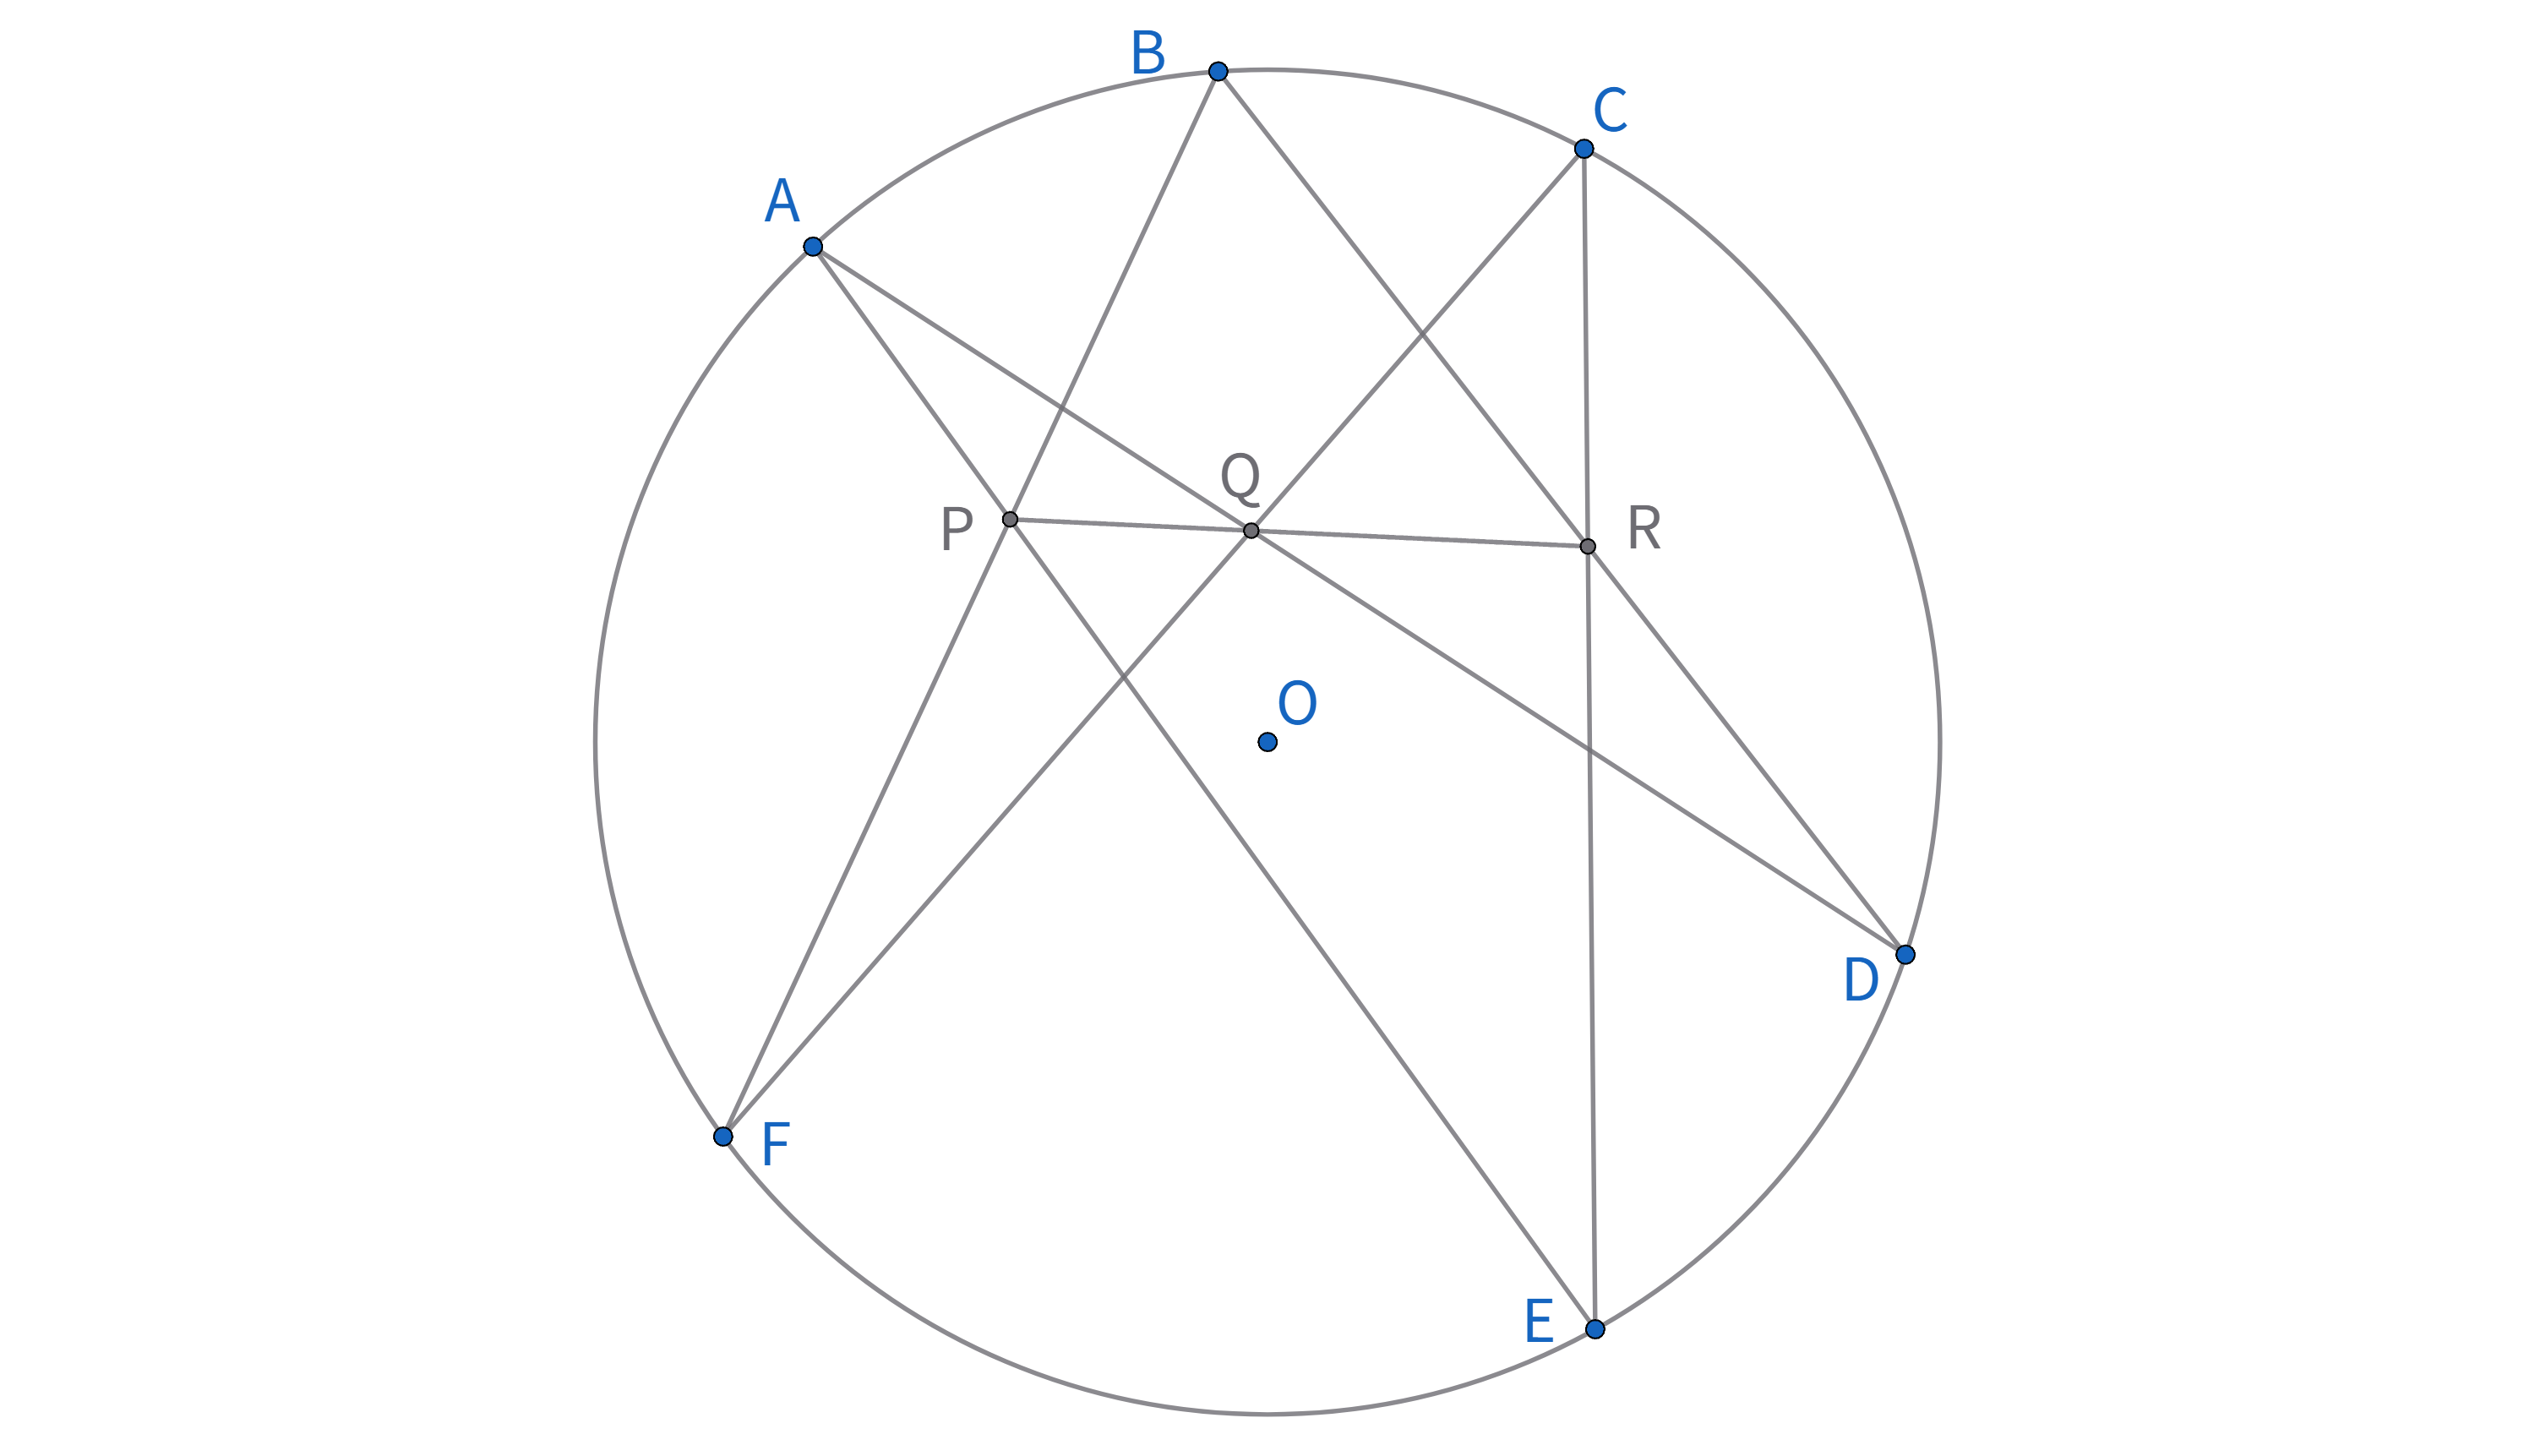
\includegraphics[width=\linewidth]{figures/帕斯卡定理.png}
    \caption{帕斯卡定理}
\end{figure}


%---------------------------------------------------
\newpage
\section{勒莫恩定理}
\begin{theorem}[勒莫恩(Lemoine)定理]
过$\triangle ABC$的三个顶点A、B、C作它外接圆O的切线,分别和BC、CA、AB所在直线交于D、E、F,则D、E、F三点共线。
\end{theorem}
\begin{figure}[H]
    \centering
    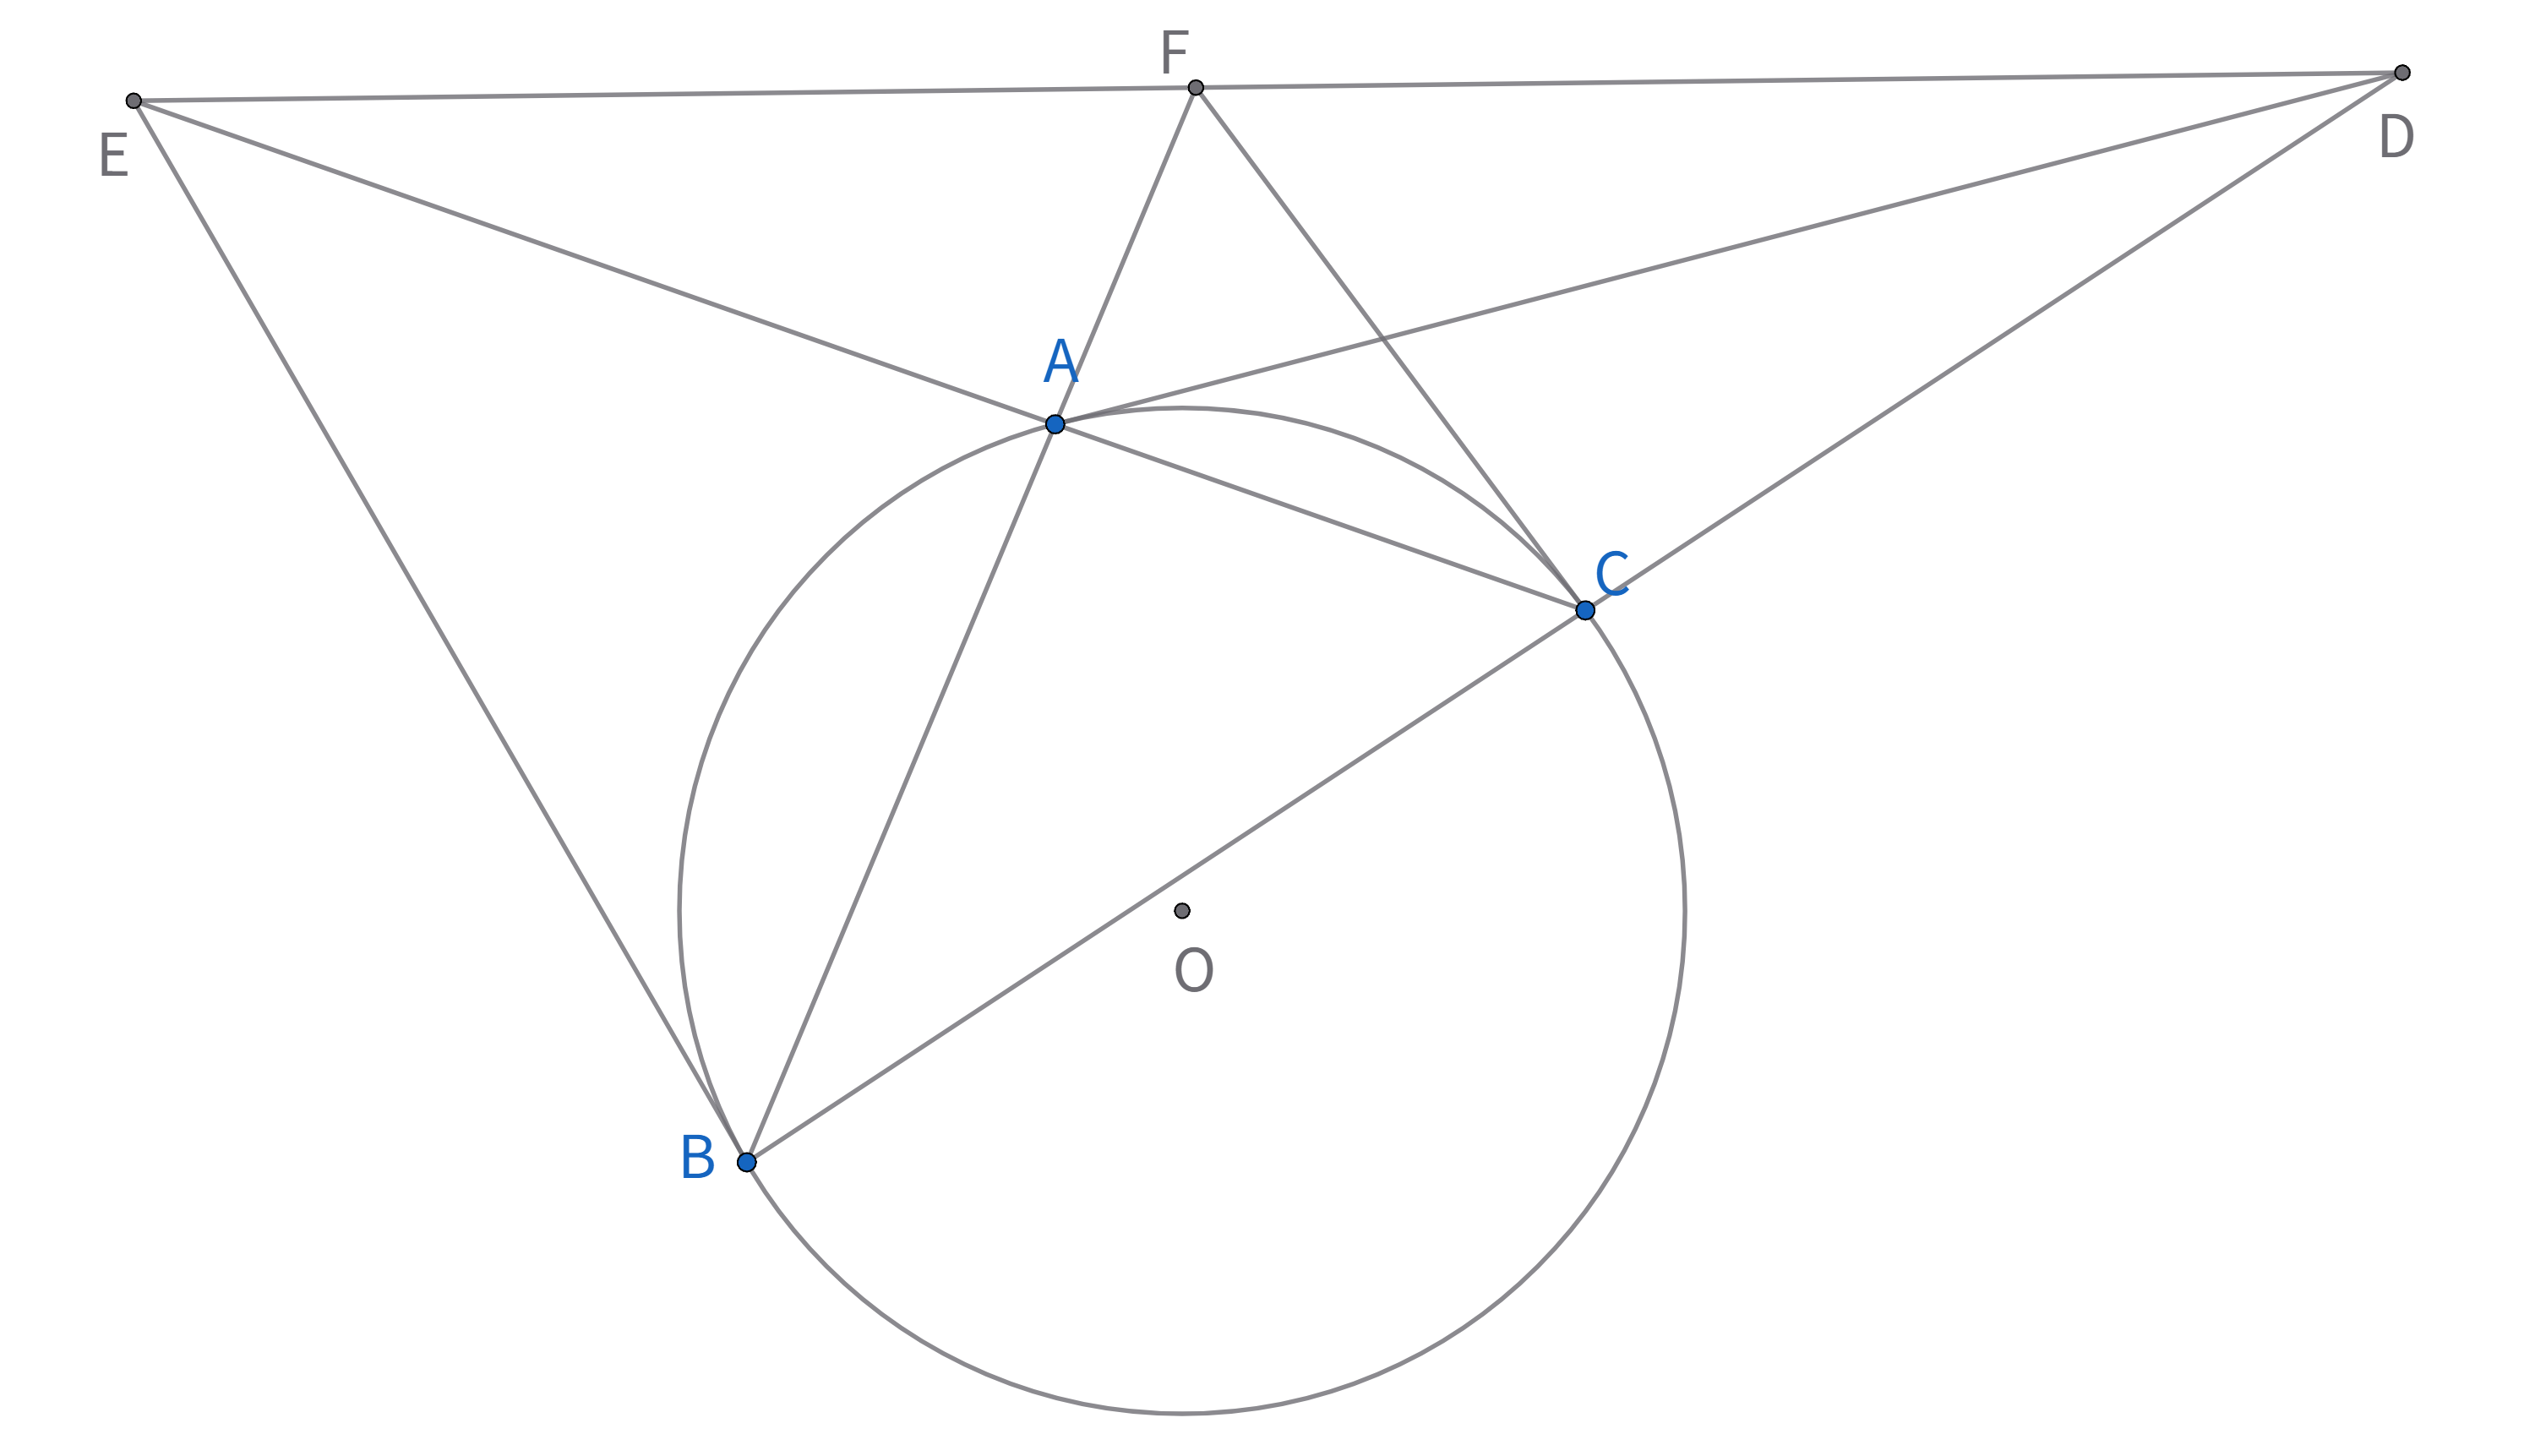
\includegraphics[width=\linewidth]{figures/勒莫恩定理.png}
    \caption{勒莫恩定理}
\end{figure}


%---------------------------------------------------
\newpage
\section{笛沙格定理}
\begin{theorem}[笛沙格(Desargues)定理]
若$\triangle ABC, \triangle DEF$ 的对应顶点连线共点(此点称为透视中心),则其对应边的交点一定共线(此线称为透视轴)。
此定理的逆定理亦成立。
满足德萨格定理的两个三角形称为透视的。
\end{theorem}
\begin{figure}[H]
    \centering
    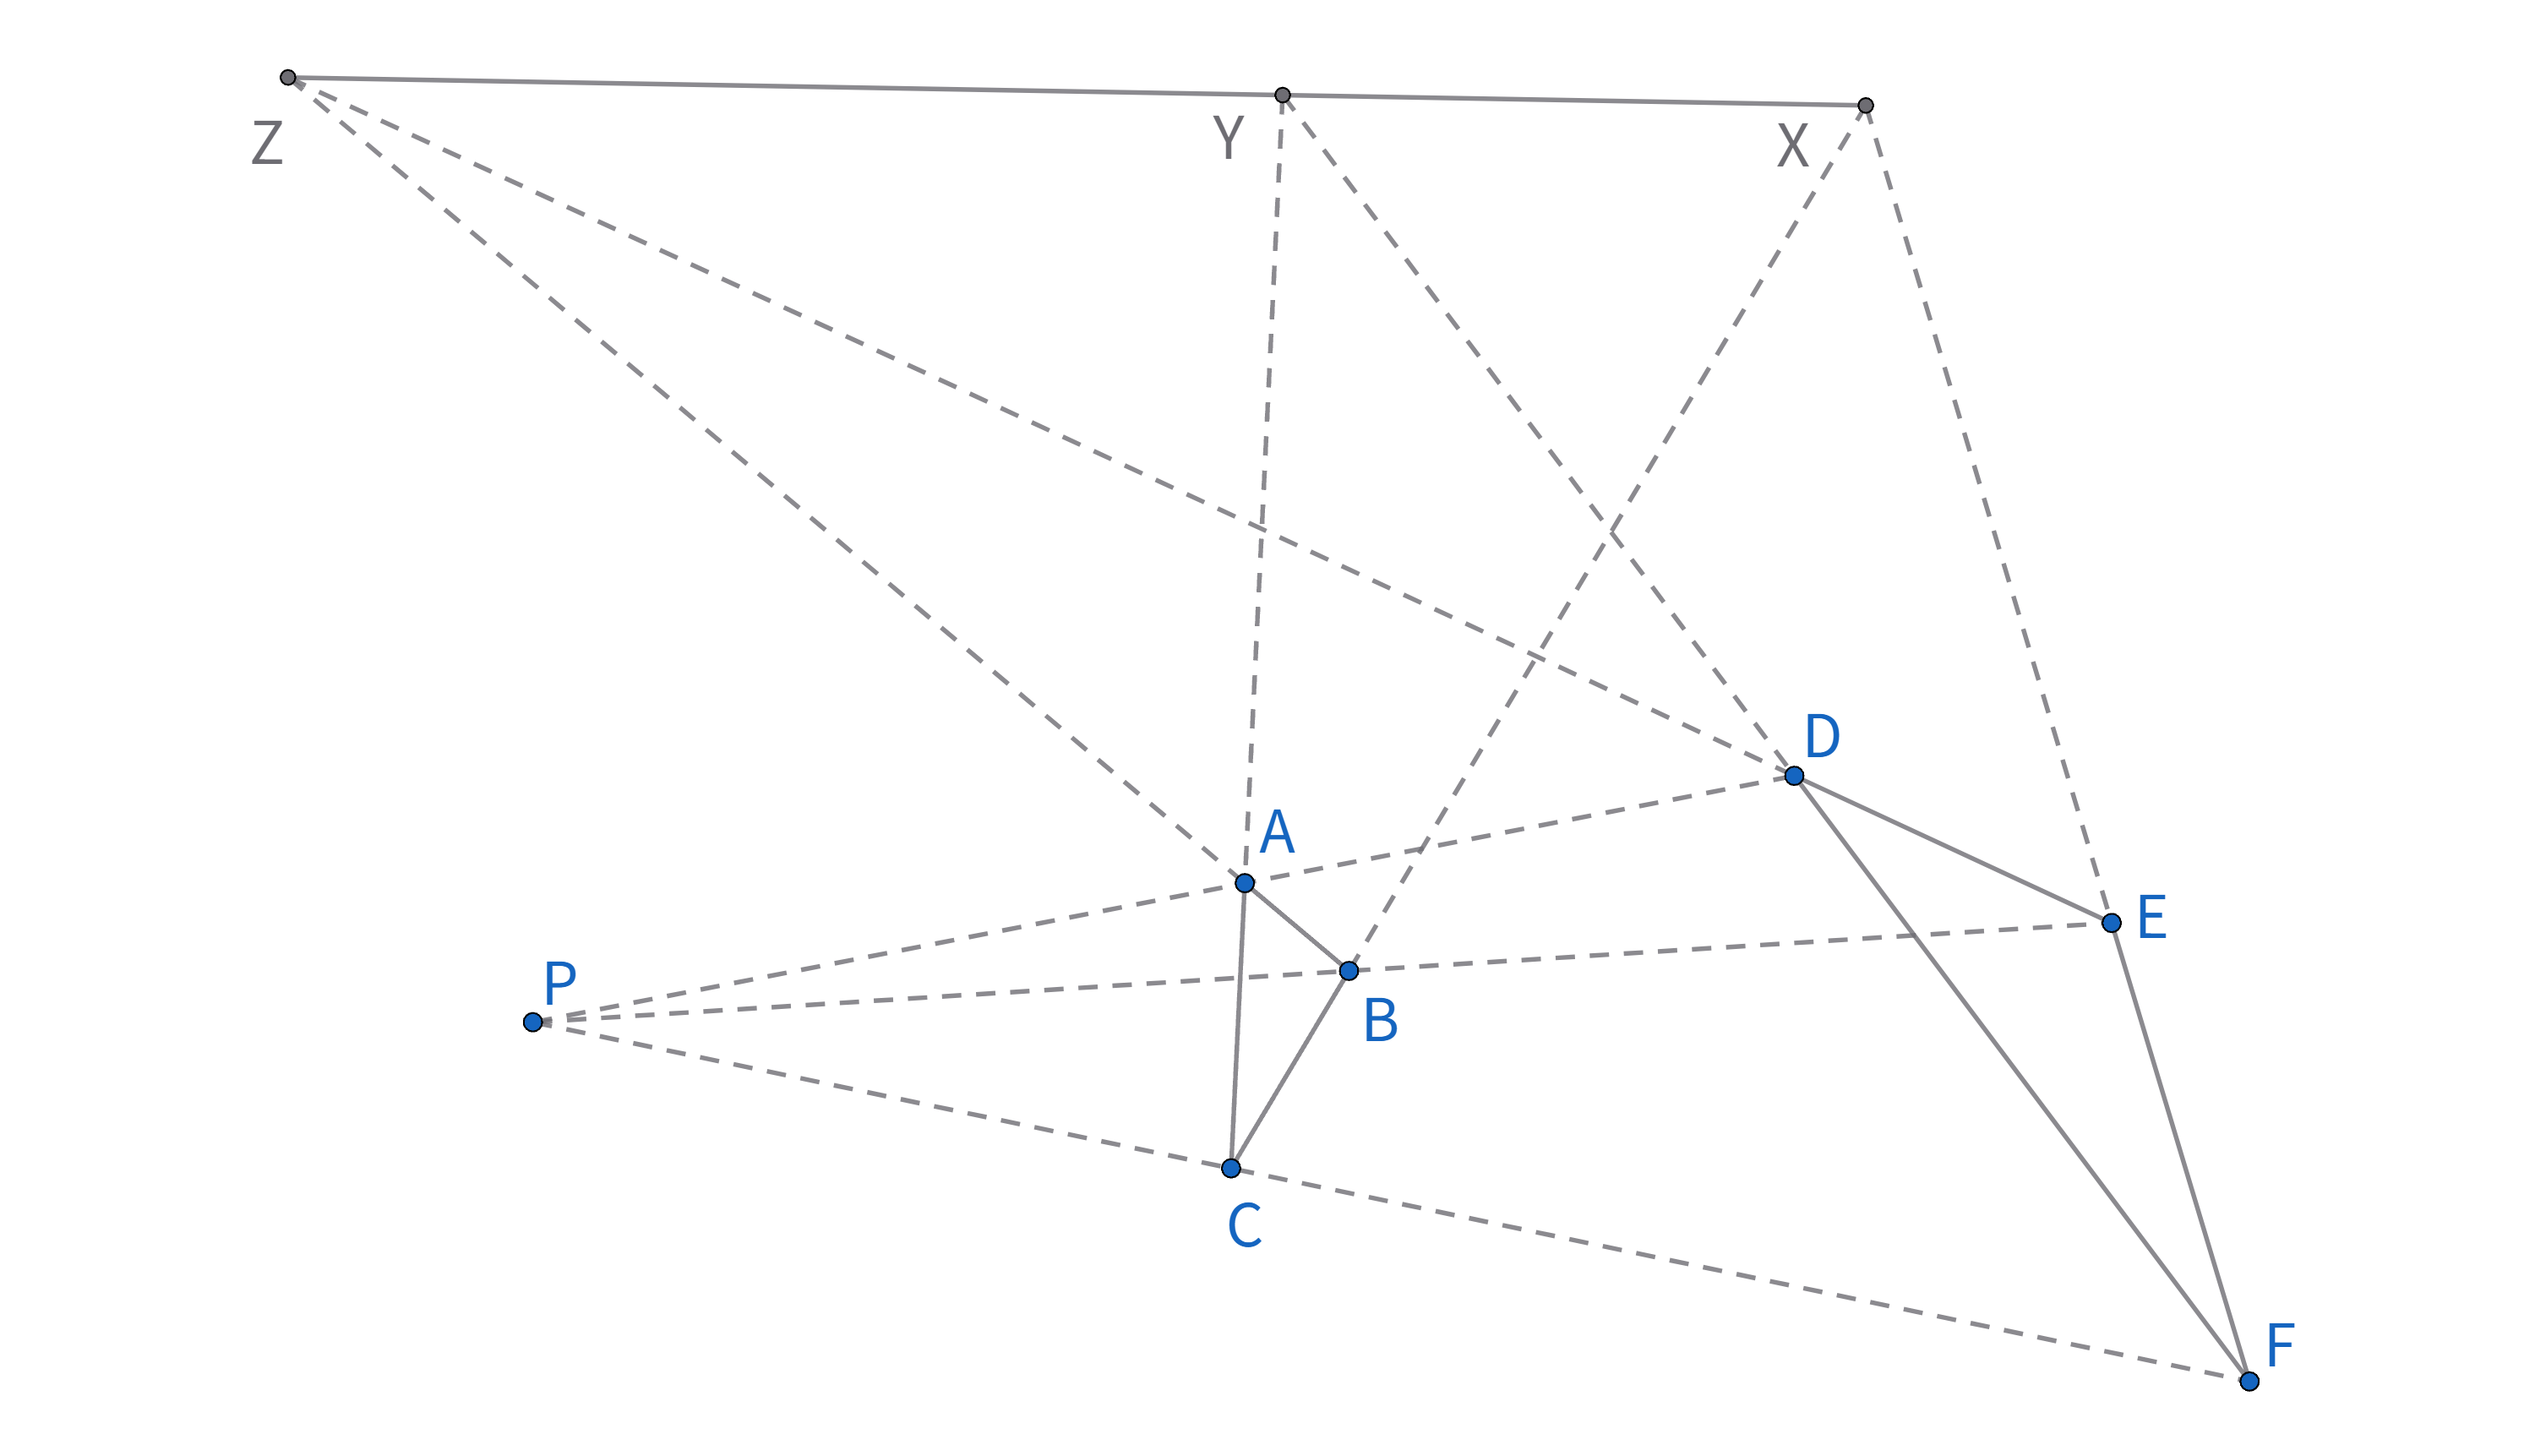
\includegraphics[width=\linewidth]{figures/笛沙格定理.png}
    \caption{笛沙格定理}
\end{figure}


%---------------------------------------------------
\newpage
\section{布拉美古塔(婆罗摩笈多)定理}
\begin{theorem}[婆罗摩笈多(Brahmagupta)定理]
圆内接四边形ABCD的对角线相互垂直,交点为M。过M做BC垂线交BC于点E,交AD于点F,则F是AD的中点。
\end{theorem}
\begin{figure}[H]
    \centering
    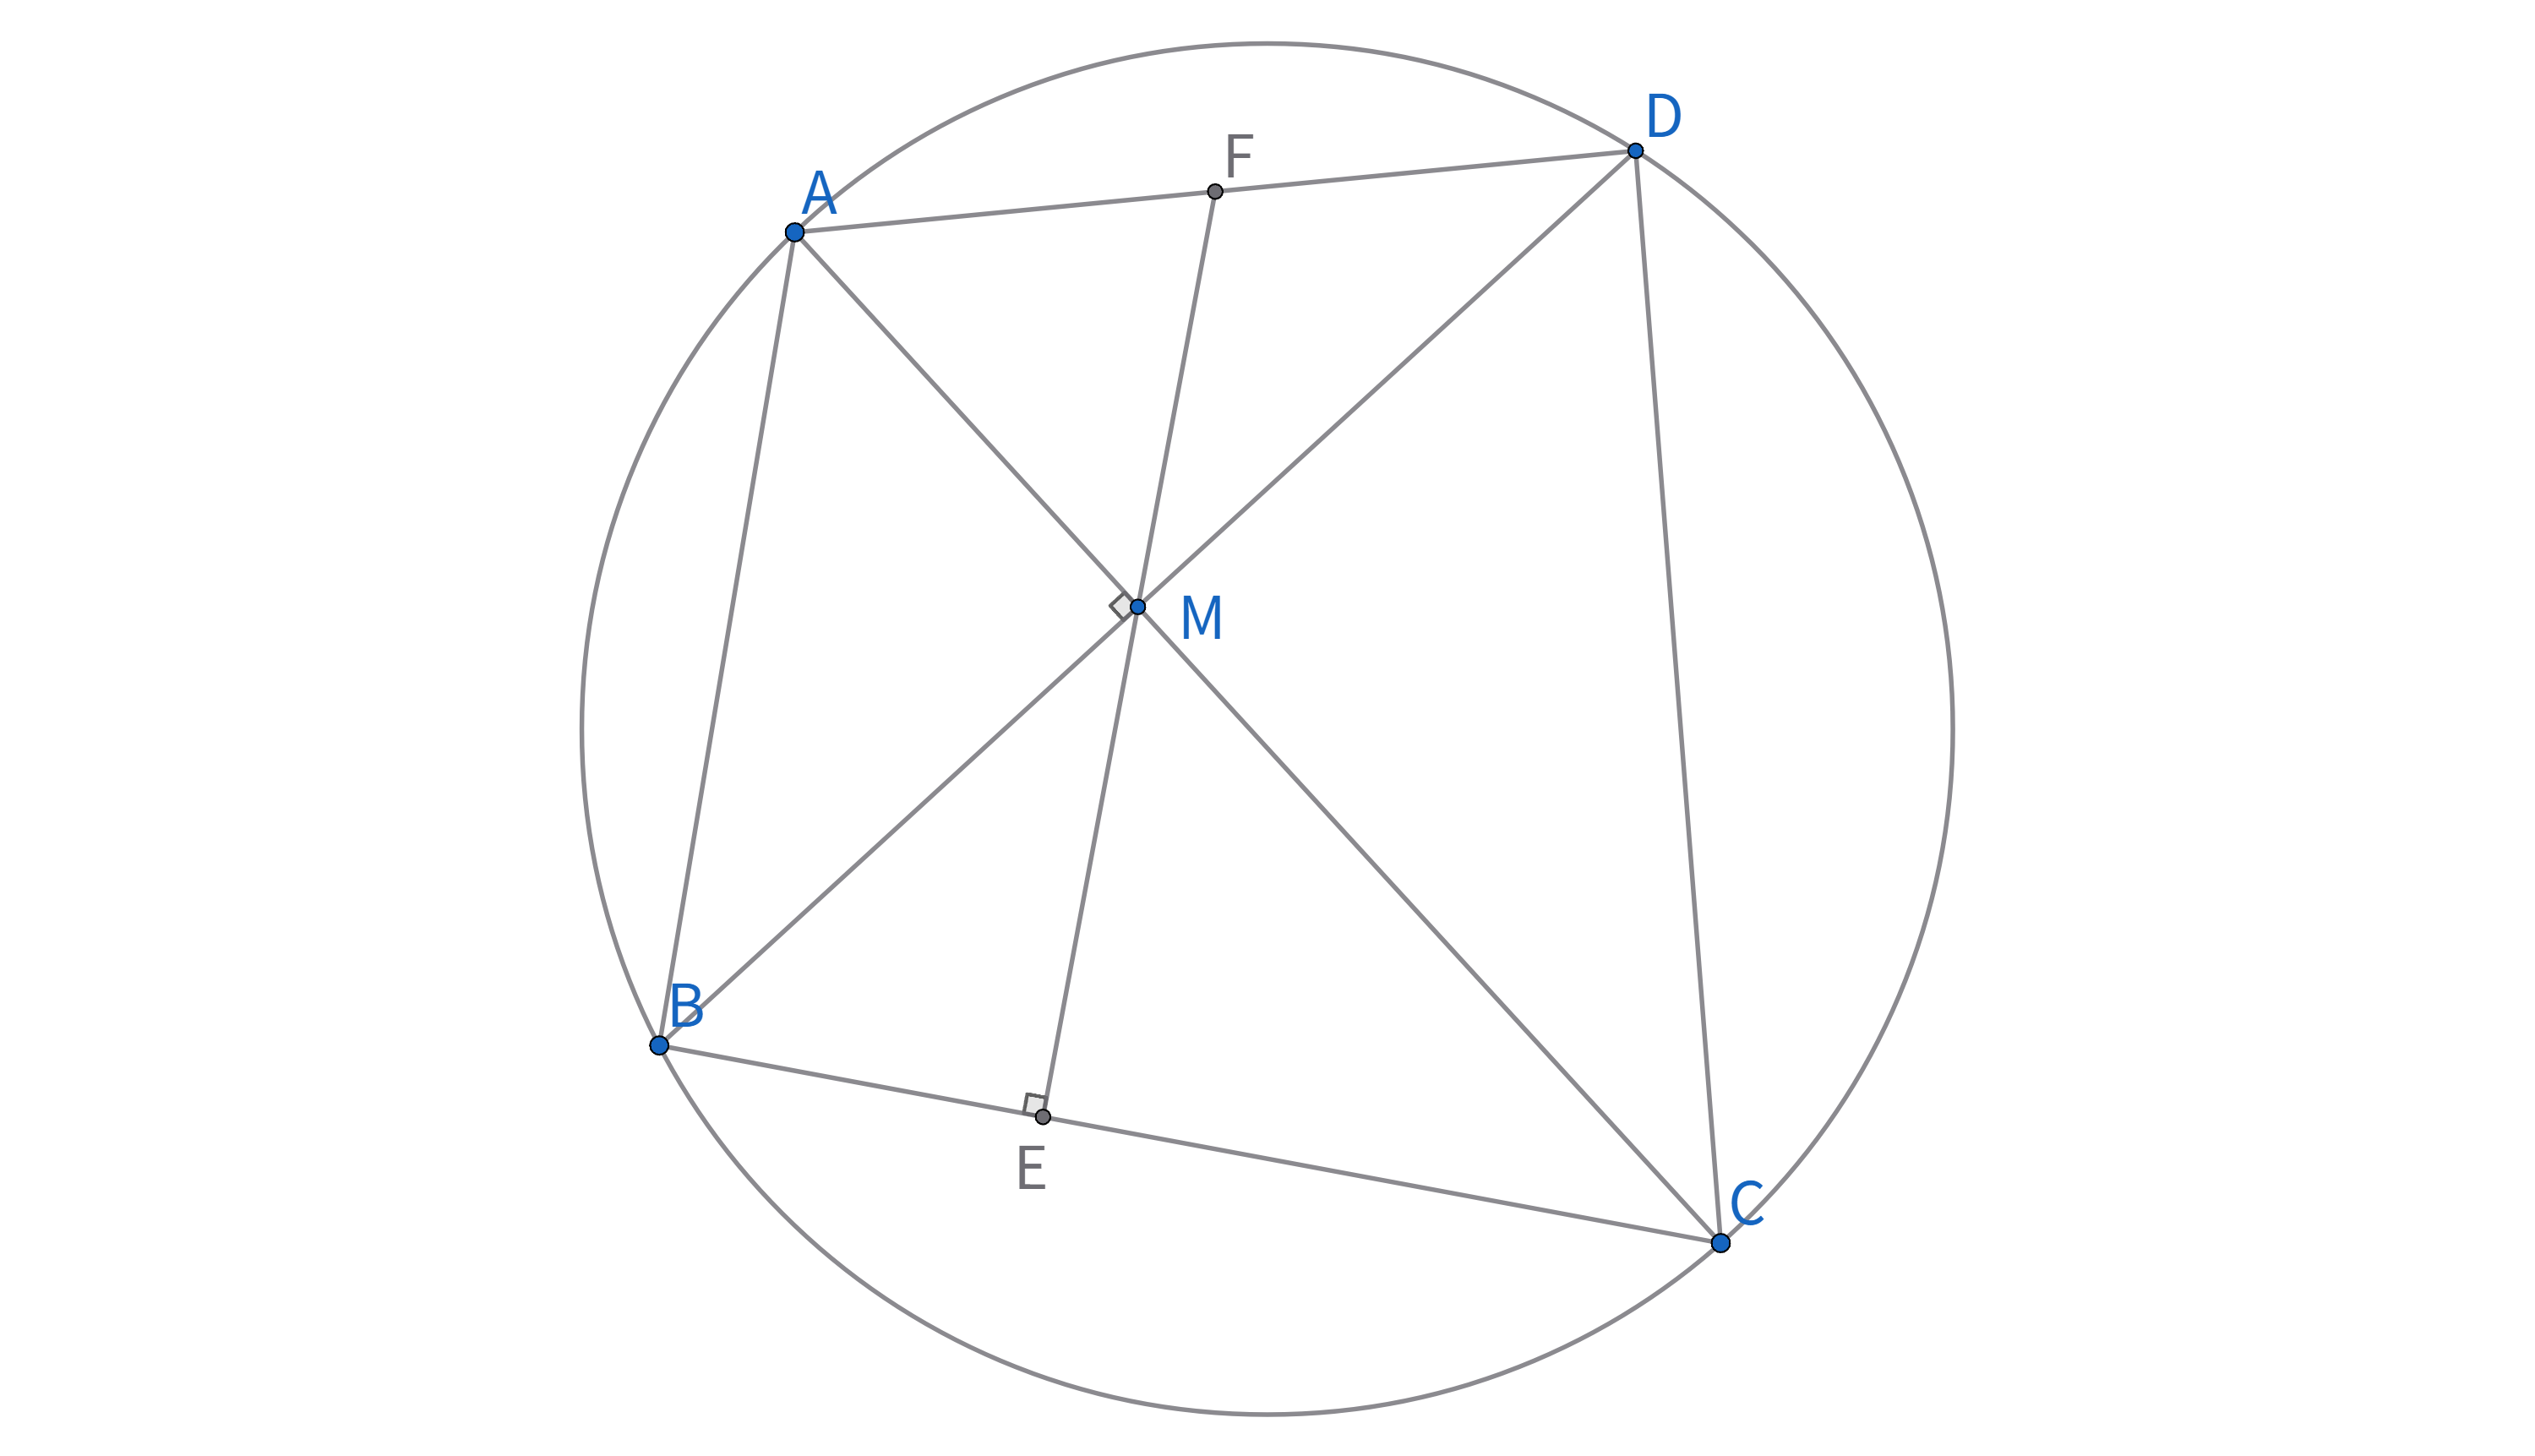
\includegraphics[width=\linewidth]{figures/婆罗摩笈多.png}
    \caption{婆罗摩笈多定理}
\end{figure}



%---------------------------------------------------
\newpage
\section{牛顿定理}
\begin{theorem}[牛顿(Newton)定理]
圆的外切四边形的对角线交点与对边切点连线交于一点。
\end{theorem}
\begin{figure}[H]
    \centering
    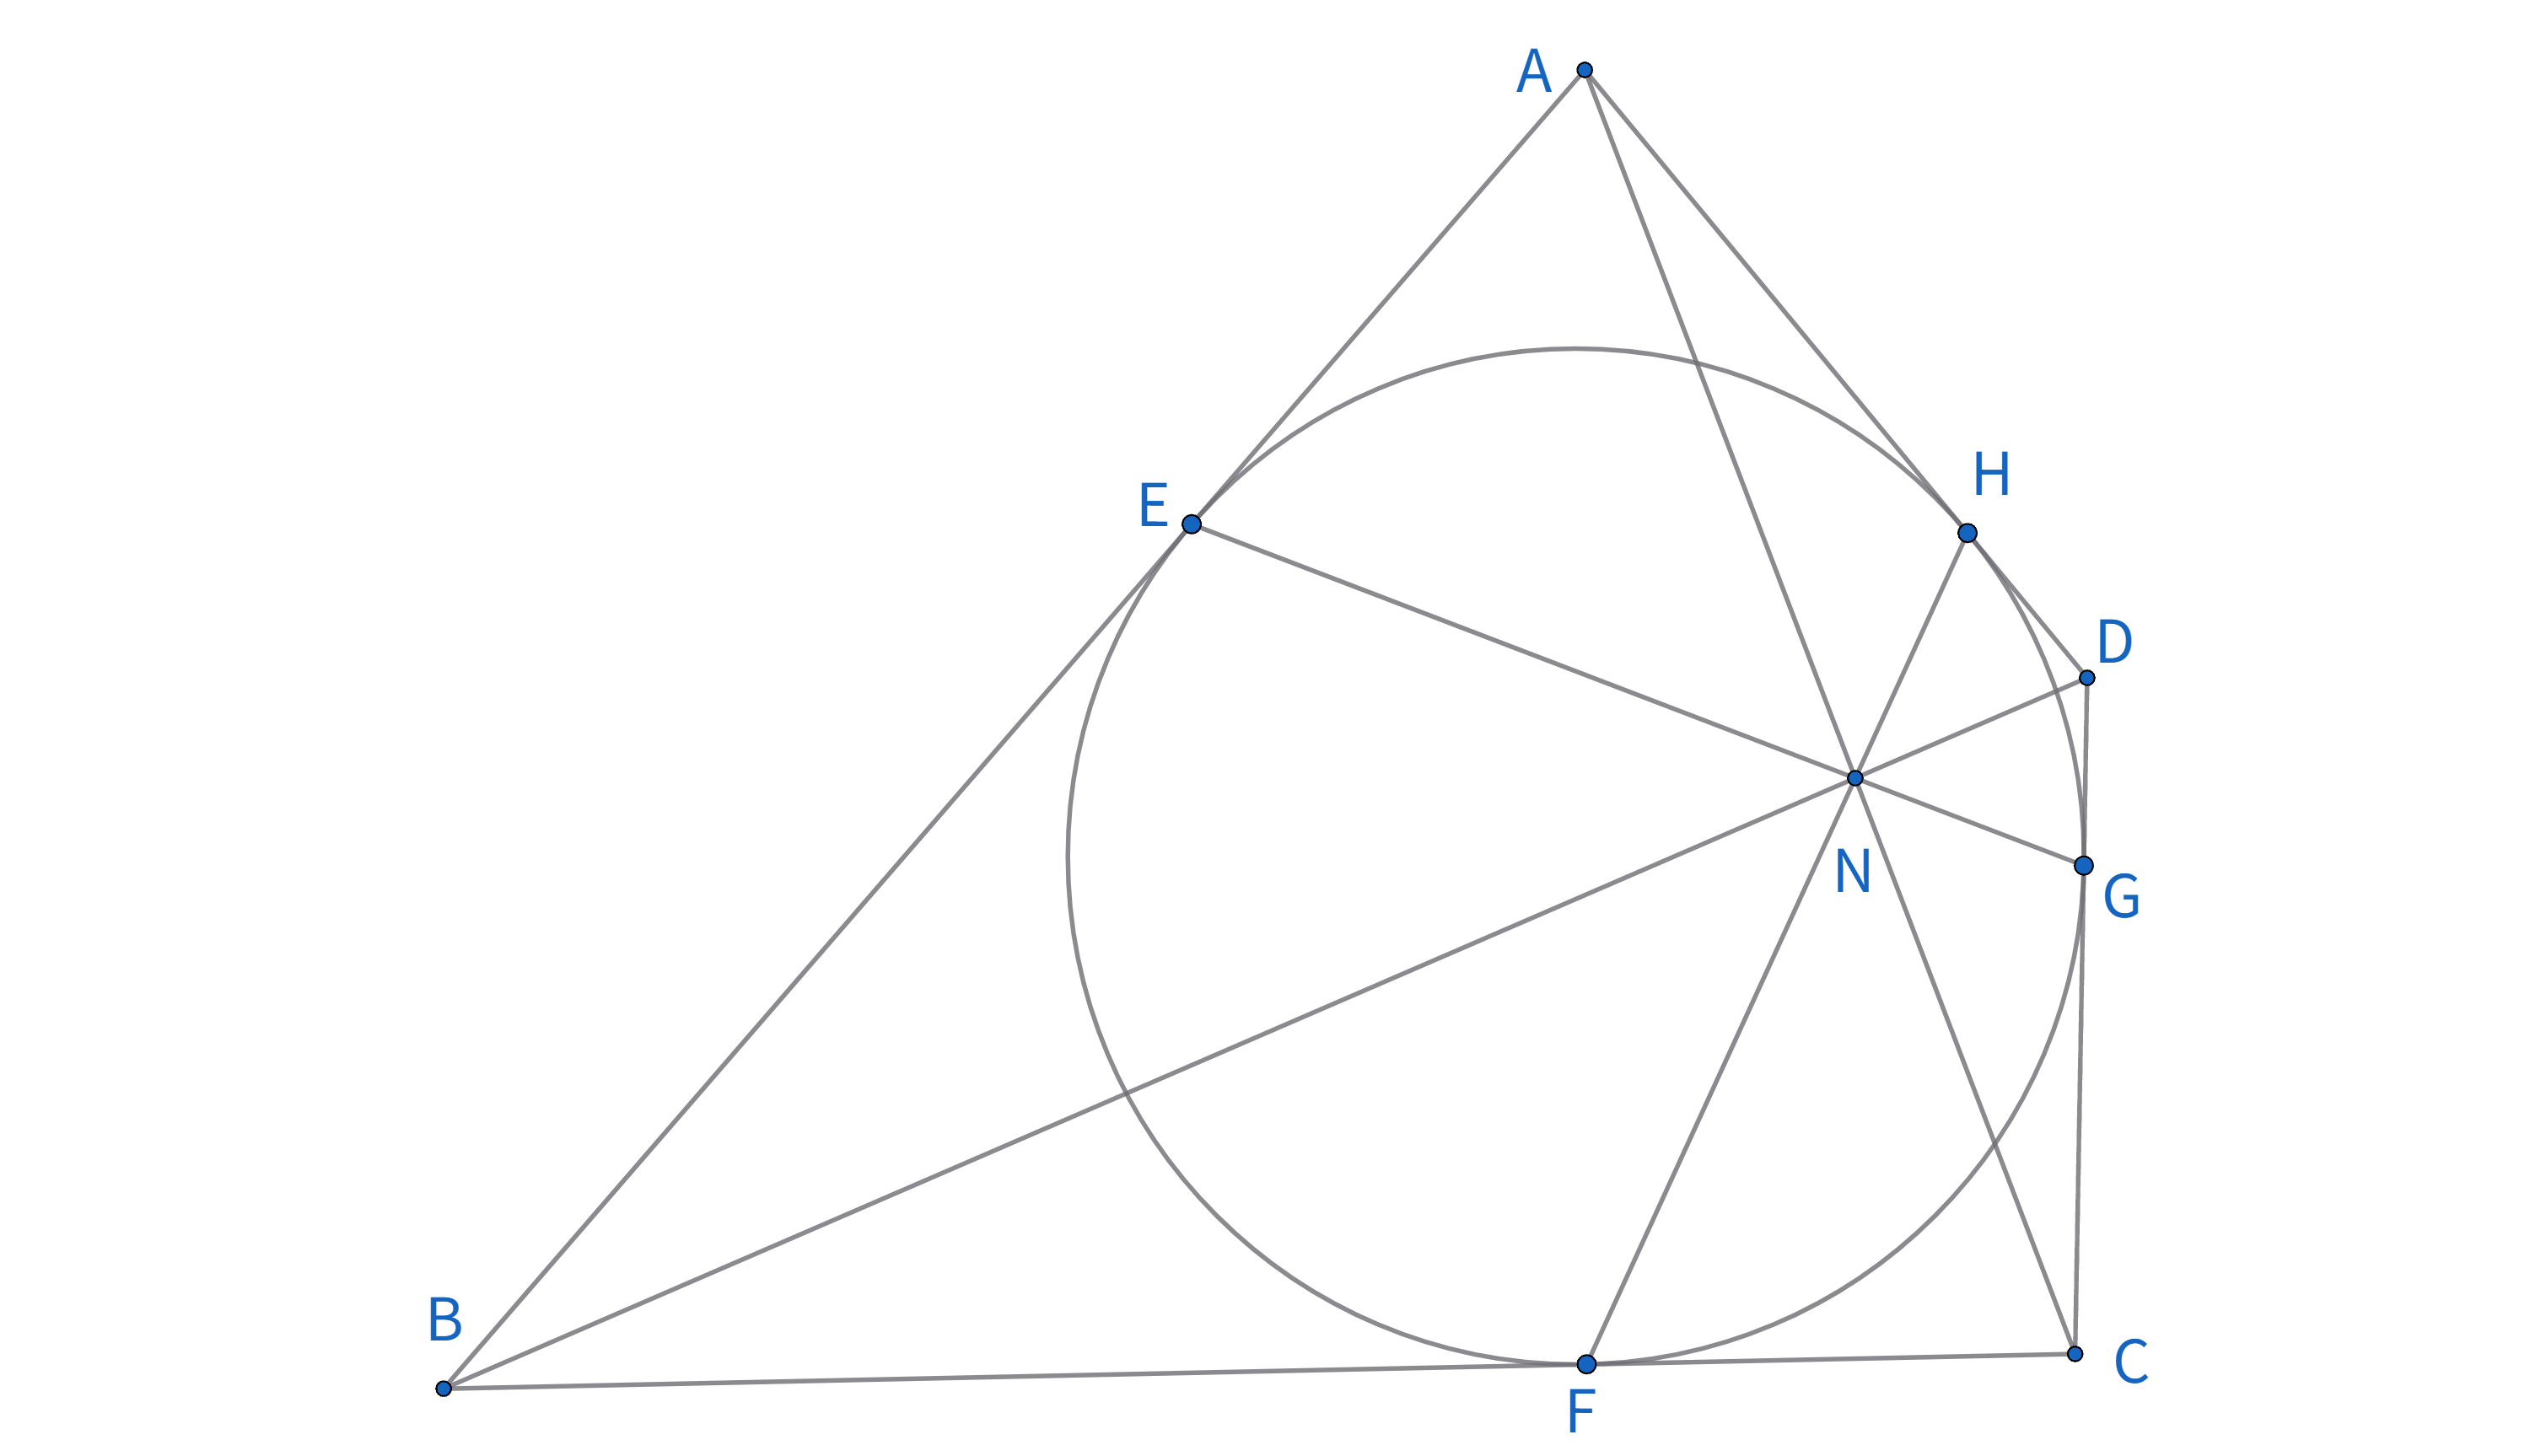
\includegraphics[width=\linewidth]{figures/牛顿定理.png}
    \caption{牛顿定理}
\end{figure}




%---------------------------------------------------
\newpage
\section{布利安香定理}
\begin{theorem}[布利安香(Brainchon)定理]
若一个六边形的六条边均与同一圆锥曲线相切,则该六边形的三条主对角线共点,该交点称为布列安桑点。\end{theorem}
\begin{figure}[H]
    \centering
    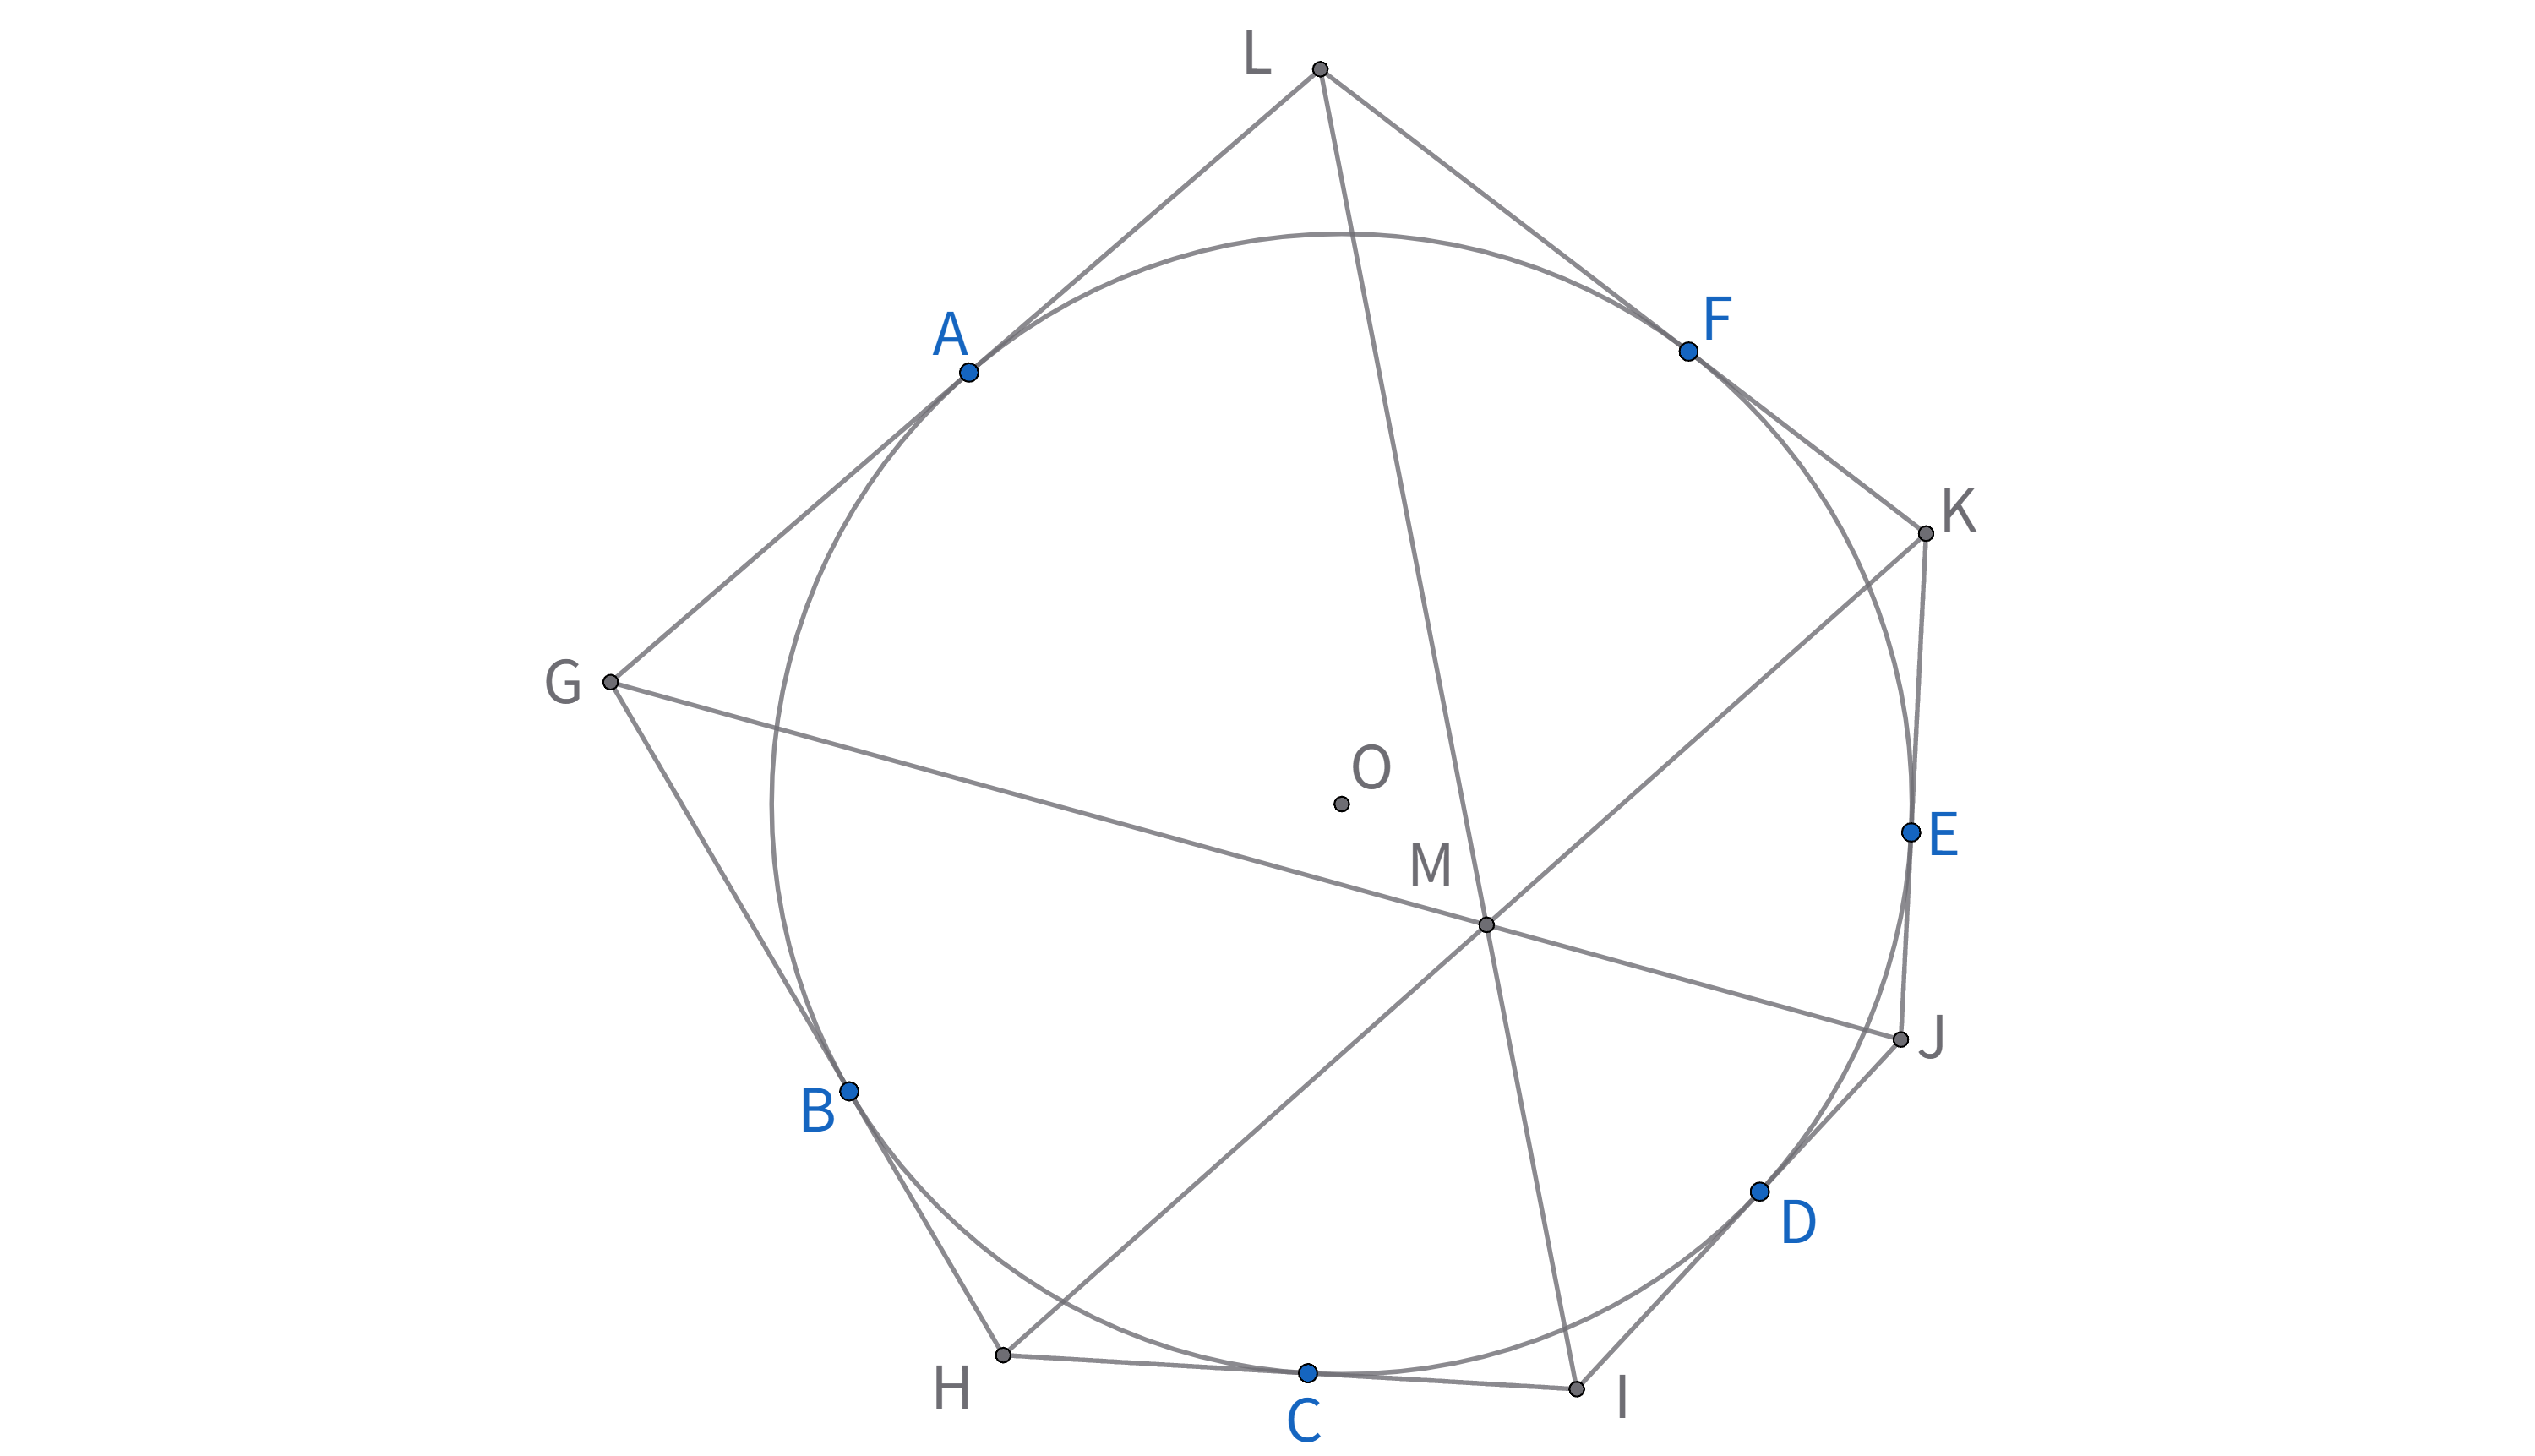
\includegraphics[width=\linewidth]{figures/布利安香.png}
    \caption{布利安香定理}
\end{figure}



% \part{三角形五心}
\section{外心}

\begin{definition}[外心]
    三角形外接圆的圆心简称为三角形的外心,通常使用O表示。
\end{definition}

\begin{figure}[H]
    \centering
    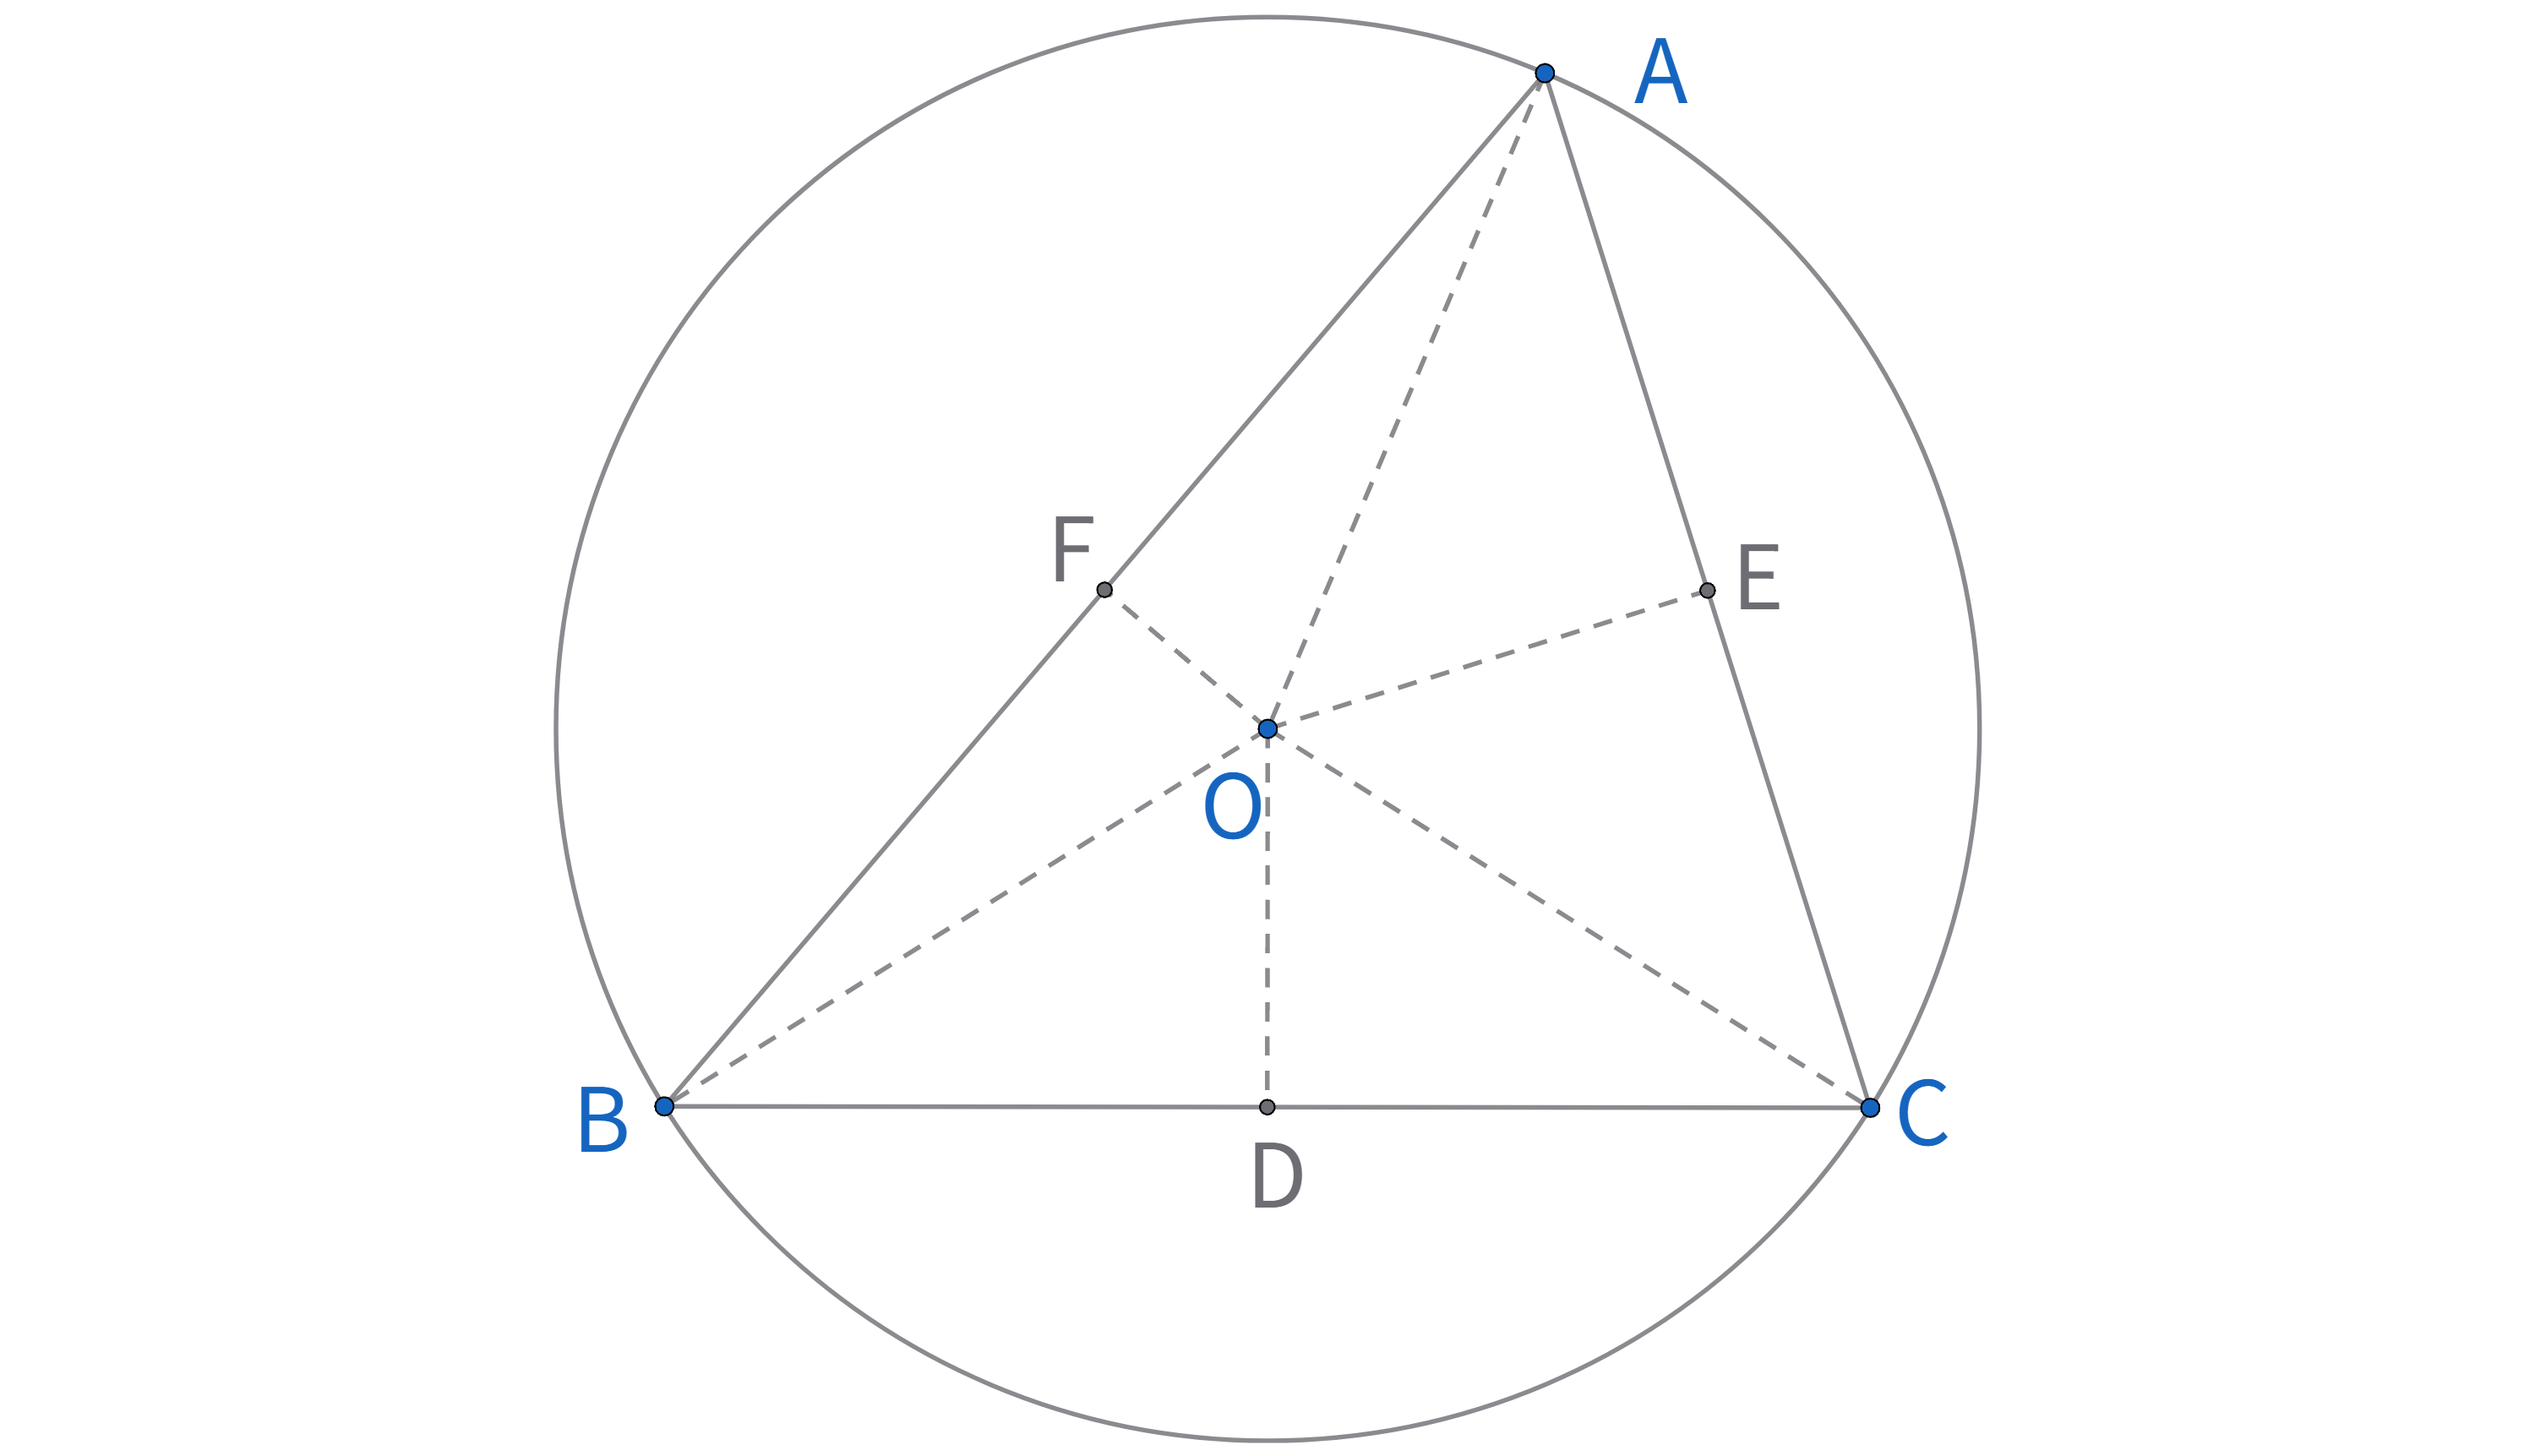
\includegraphics[width=0.8\linewidth]{figures/三角形五心/外心.png}
    \caption{外心}
\end{figure}

\begin{proposition}[外心性质]
    三角形外心具有如下性质。
    
    (1) 三角形的外心是三条边中垂线的交点。

    (2) 平面内一点是三角形外心的充分必要条件为:该点到三顶点的距离相等。

    (3) 锐角三角形的外心在形内,直角三角形的外心为斜边中点,钝角三角形的外心在形外。
\end{proposition}

\begin{exercise}
    用$\triangle ABC$外接圆半径长$R$以及三顶角的正弦函数表示所有线段长。
\end{exercise}


%--------------------------------------------------------------
\newpage 
\section{内心}

\begin{definition}[内心]
    三角形内切圆的圆心简称为三角形的内心,通常使用I表示。
\end{definition}

\begin{figure}[H]
    \centering
    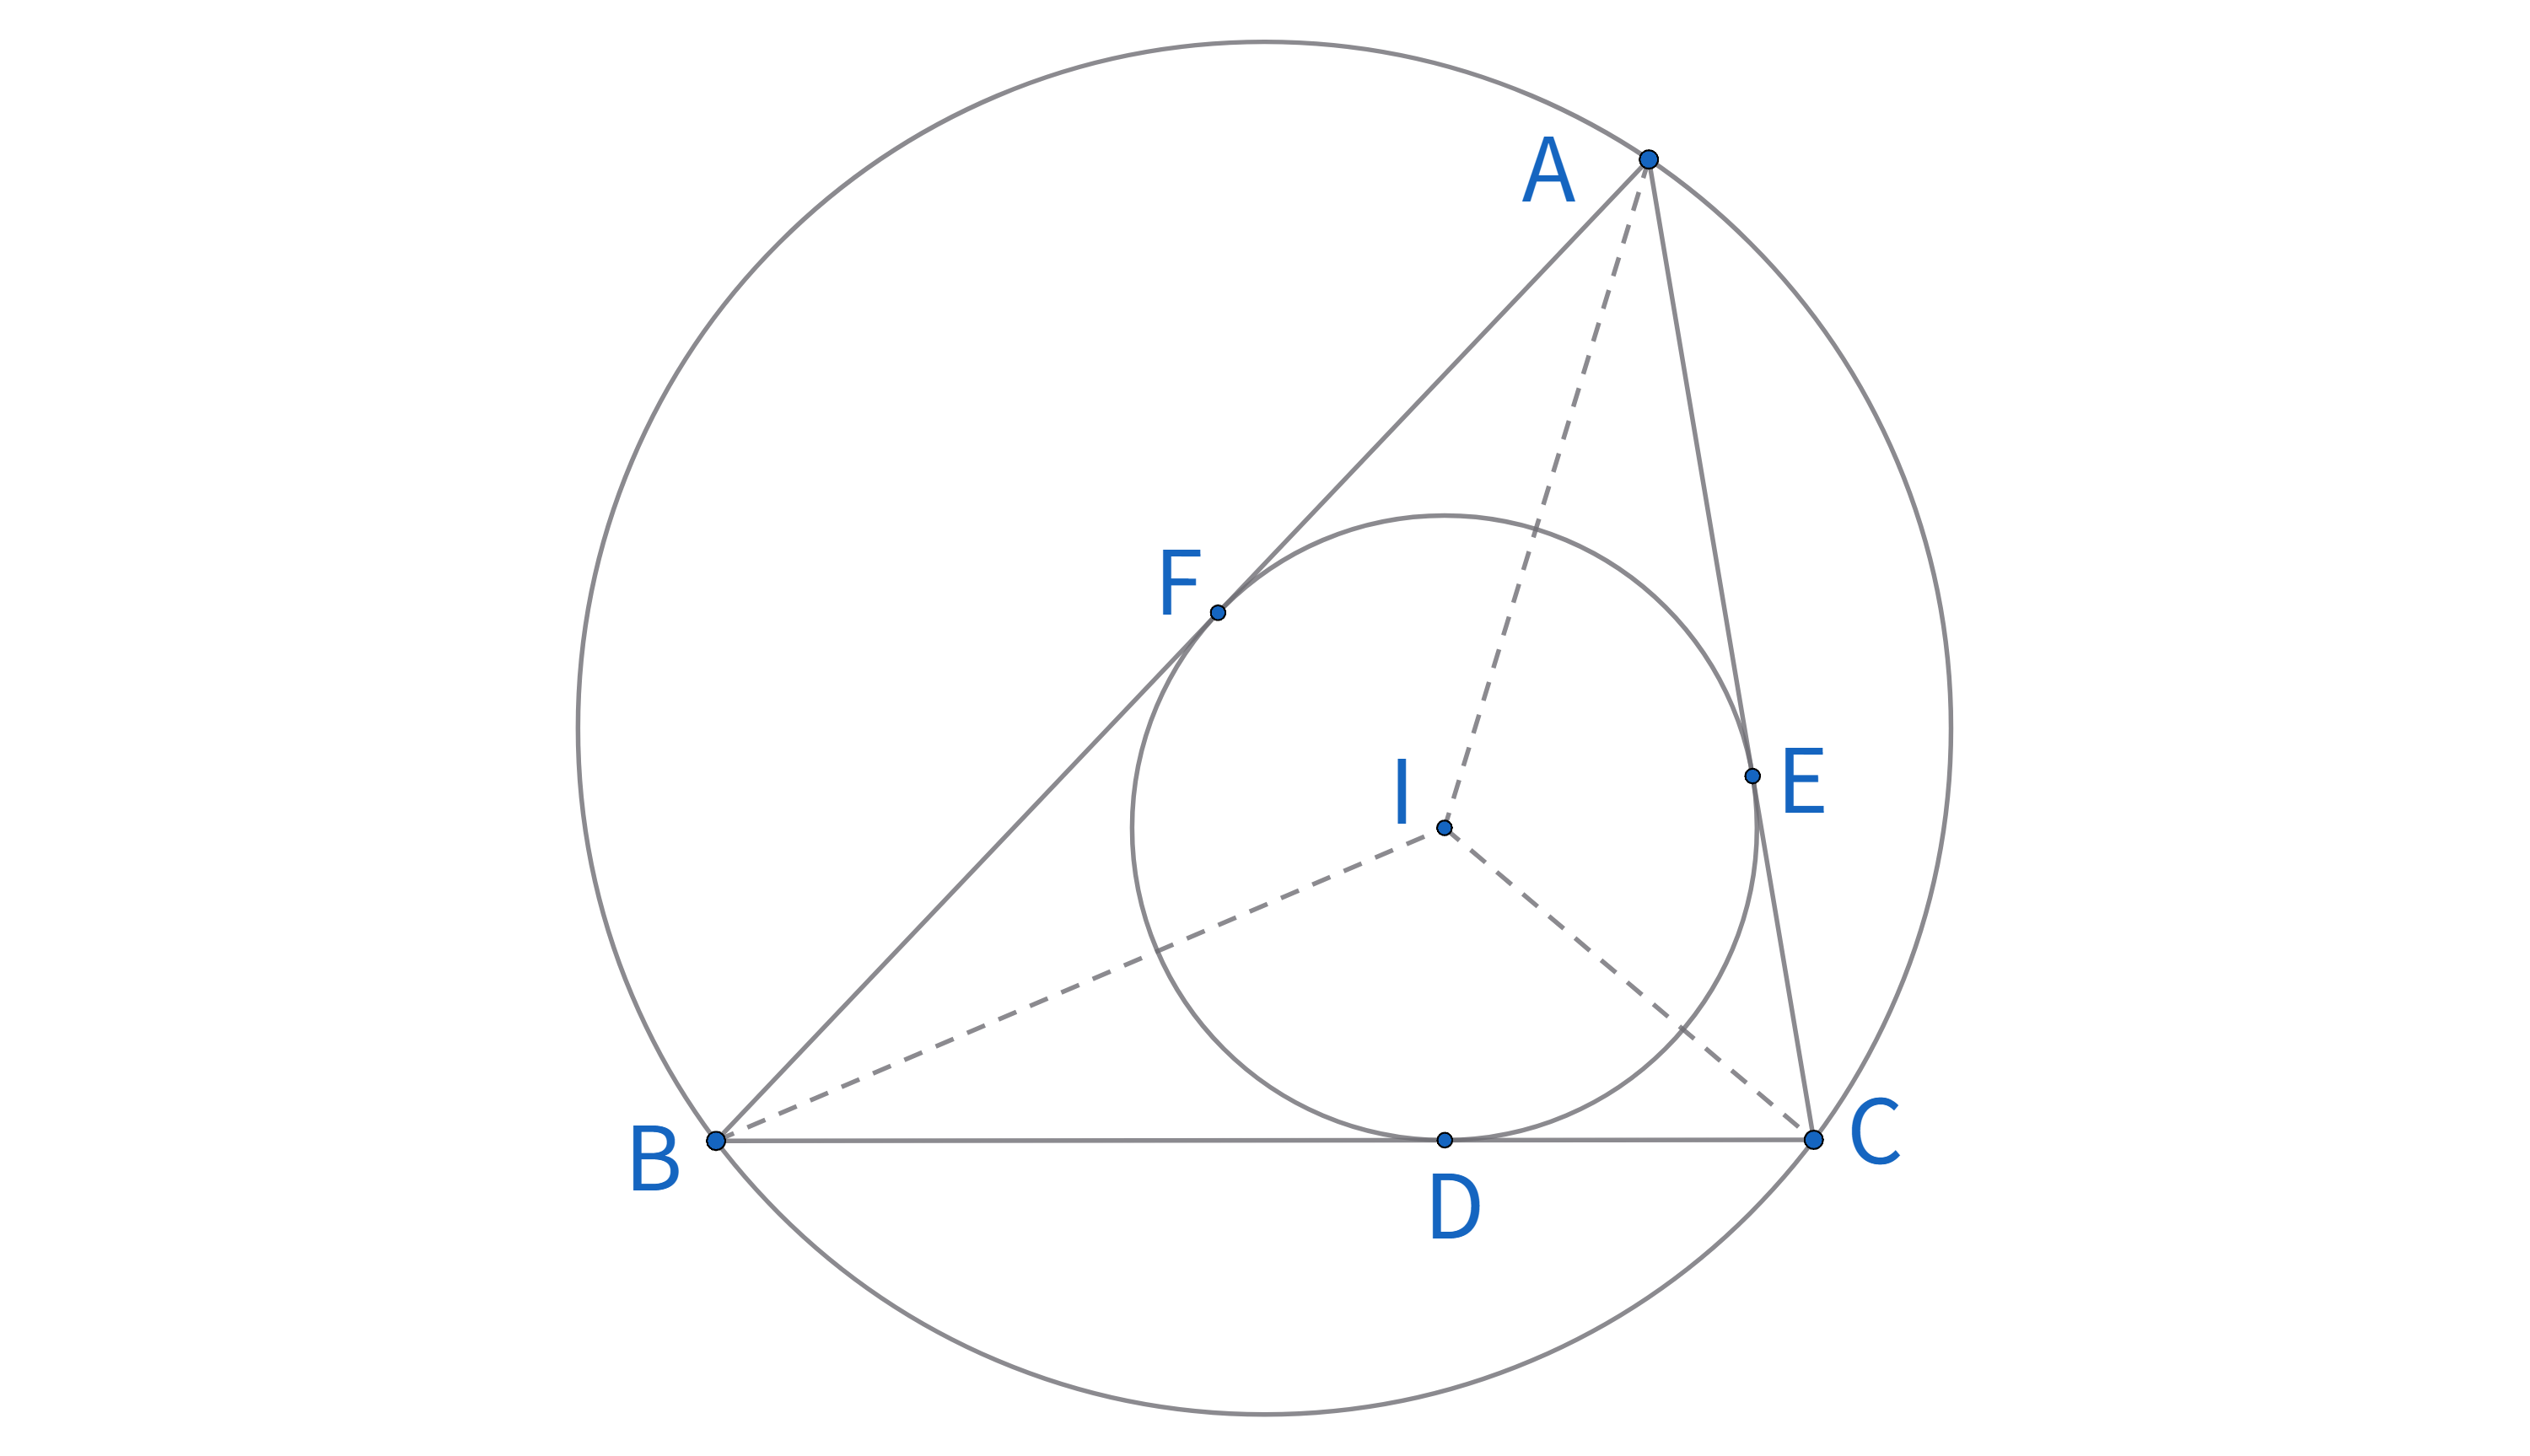
\includegraphics[width=0.8\linewidth]{figures/三角形五心/内心.png}
    \caption{内心}
\end{figure}

\begin{proposition}[内心性质]
    三角形内心具有如下性质。
    
    (1) 三角形的内心是三条内角平分线的交点。

    (2) 内心到三边的距离相等。

    (3) 平面内一点I是三角形$\triangle ABC$内心的充分必要条件为:
    $$\angle BIC = 90^\circ +\frac{1}{2}A,\quad \angle AIC = 90^\circ +\frac{1}{2}B,
    \quad \angle AIB =90^\circ +\frac{1}{2}C.$$

\end{proposition}


\begin{proposition}[切线长性质]
    设D、E、F分别为内切圆I在BC、CA、AB上的切点,则
    $$
    \begin{aligned}
    AE&=AF=s-a = \frac{1}{2}(b+c - a),\\
    BF&=BD=s - b =\frac{1}{2}(a+c - b),\\
    CD&=CE=s - c= \frac{1}{2}(a+b - c).
    \end{aligned}
    $$
\end{proposition}



\newpage 
\begin{theorem}[鸡爪定理]
    对平面内任意$\triangle ABC$,O、I分别为其外心和内心。设AI延长线与圆O相交于D,
    D为$\overset{{\frown}}{BC}$的中点,并且满足
    $$DB=DI=DC.$$
\end{theorem}

\begin{figure}[H]
    \centering
    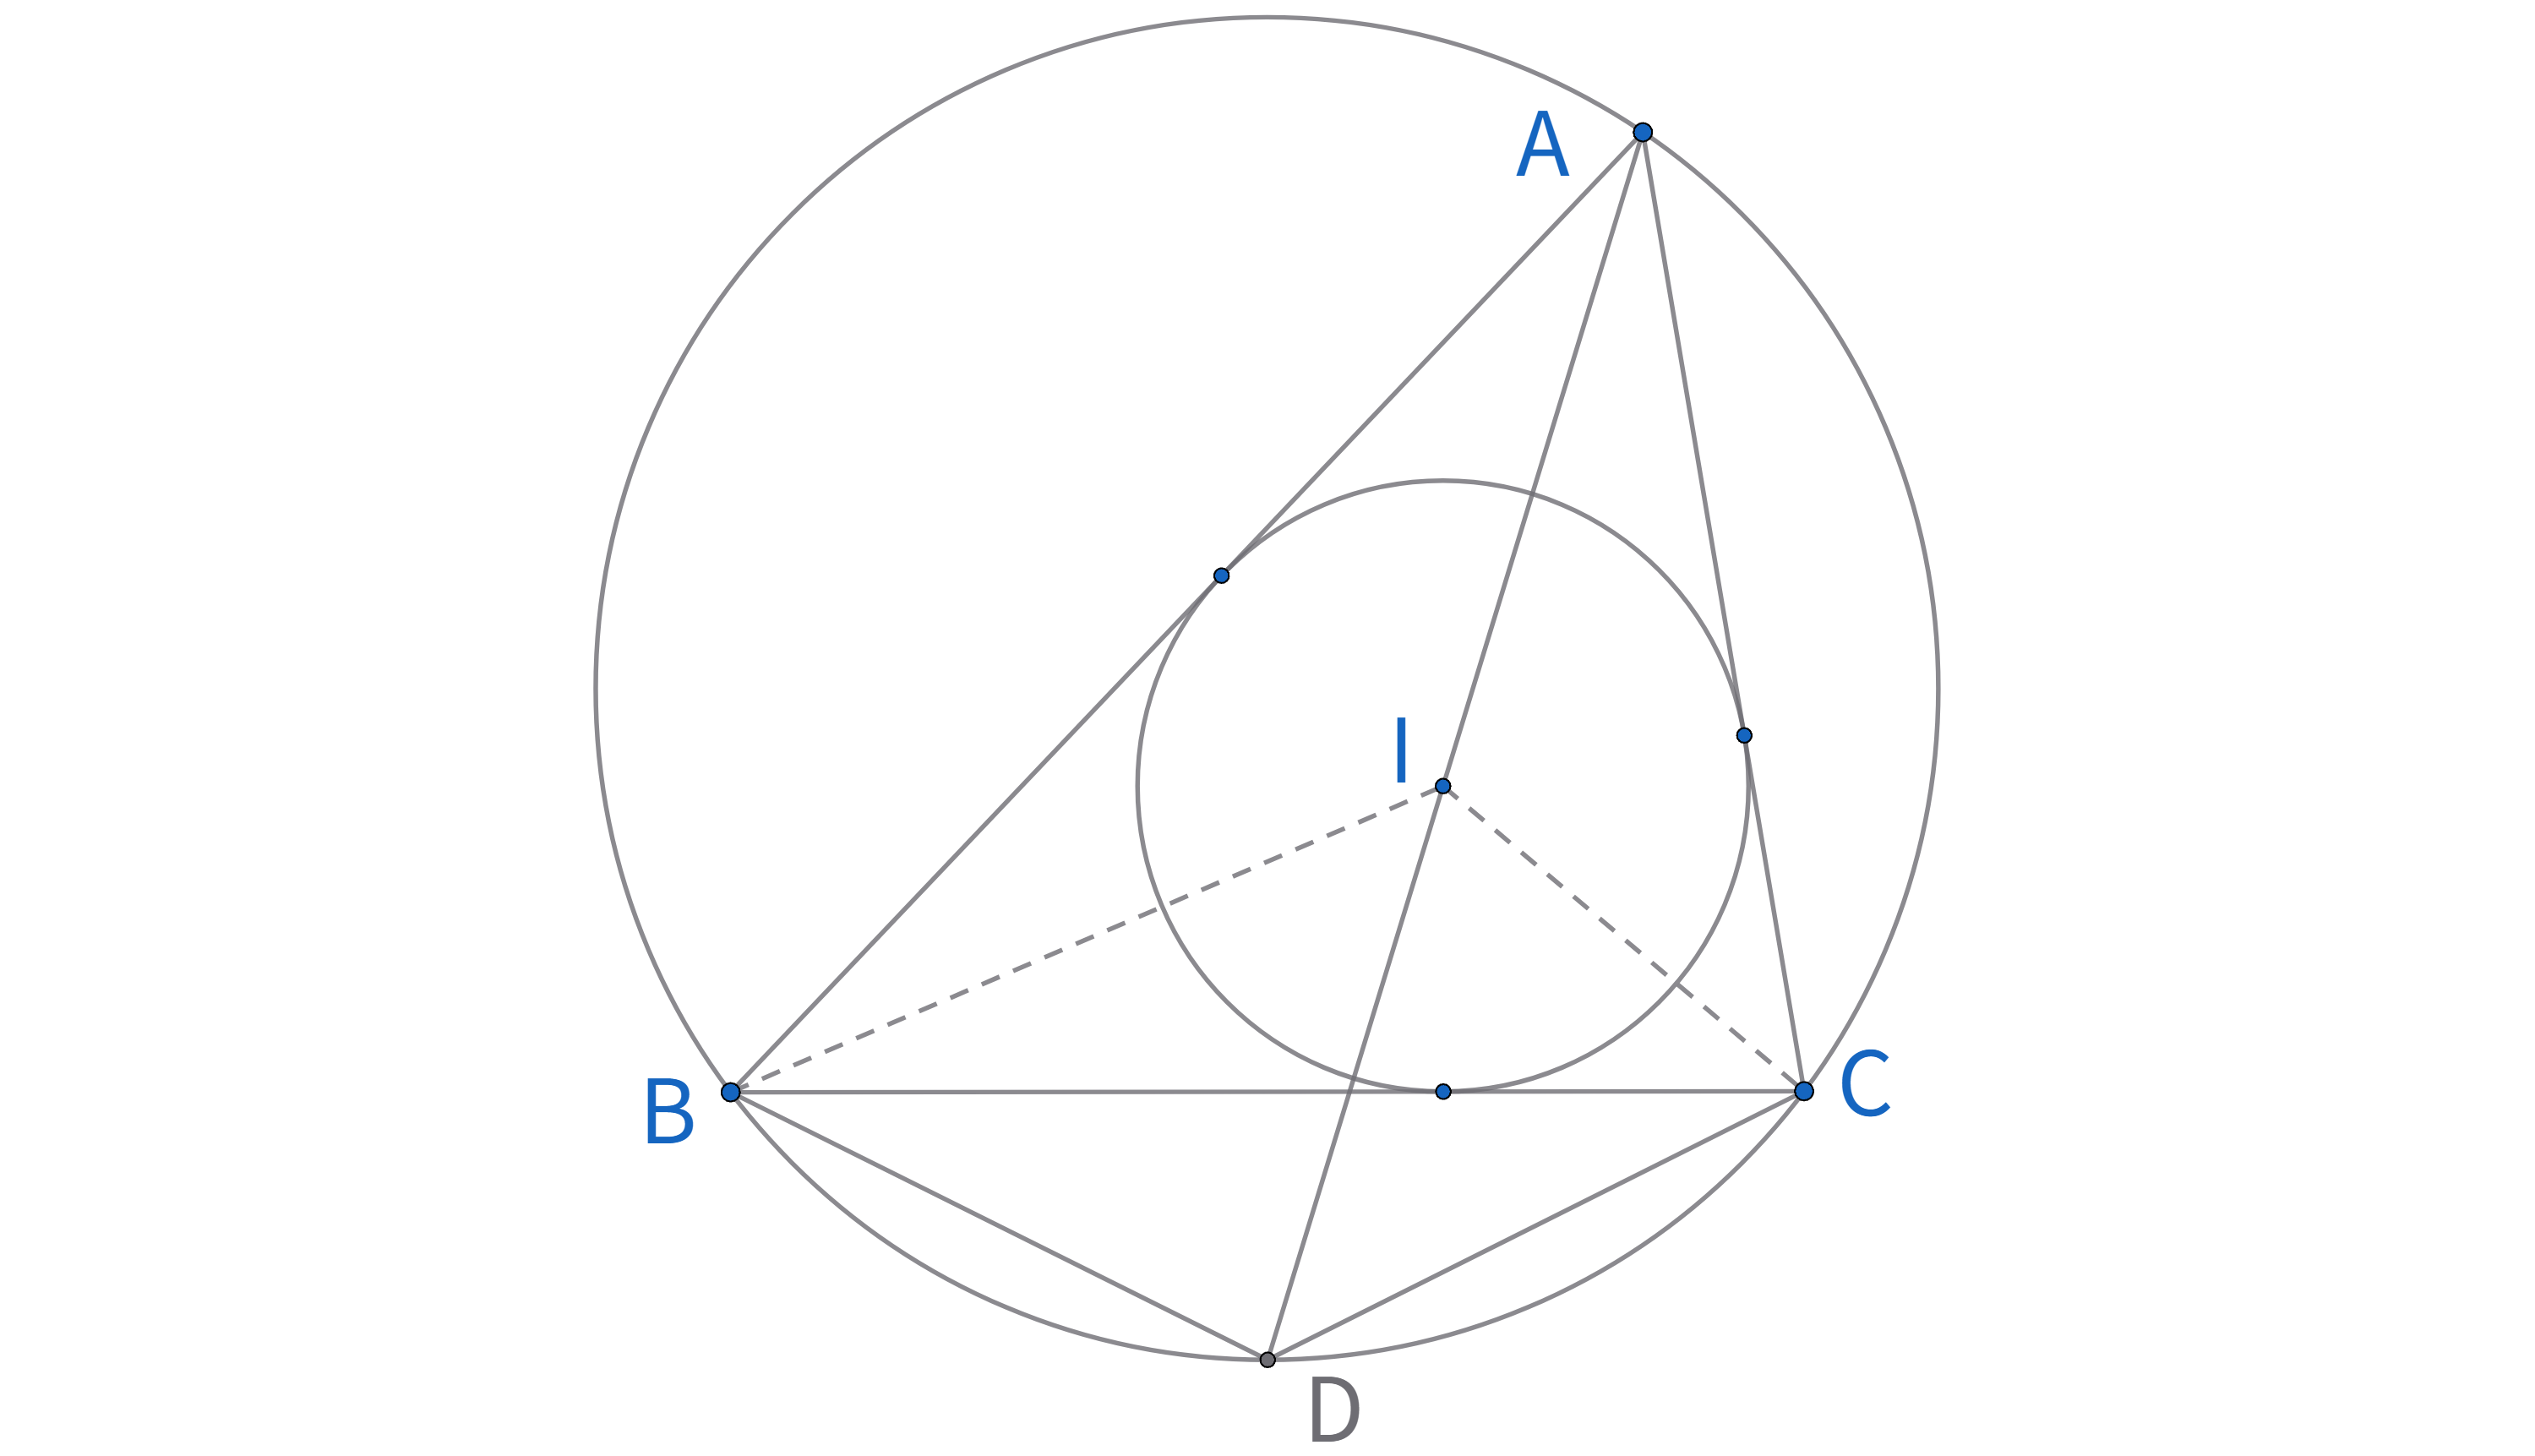
\includegraphics[width=0.8\linewidth]{figures/三角形五心/鸡爪定理.png}
    \caption{鸡爪定理}
\end{figure}

\begin{exercise}
    计算$\angle IBD, \angle ICD, \angle BID, \angle CID$。
\end{exercise}
\begin{exercise}
    表示$\triangle ABC$内切圆半径长。
\end{exercise}
\begin{exercise}
    设$\triangle DEF$为切点三角形,表示$\triangle DEF$的三边长和三顶角大小。
\end{exercise}
\begin{exercise}[内外径的欧拉定理]
    $\triangle ABC$的外接圆半径和内切圆半径分别为$R,r.$ 若$O,I$分别是二者的圆心,则$OI^2 = R(R-2r).$
\end{exercise}


% \begin{figure}[H]
%     \centering
%     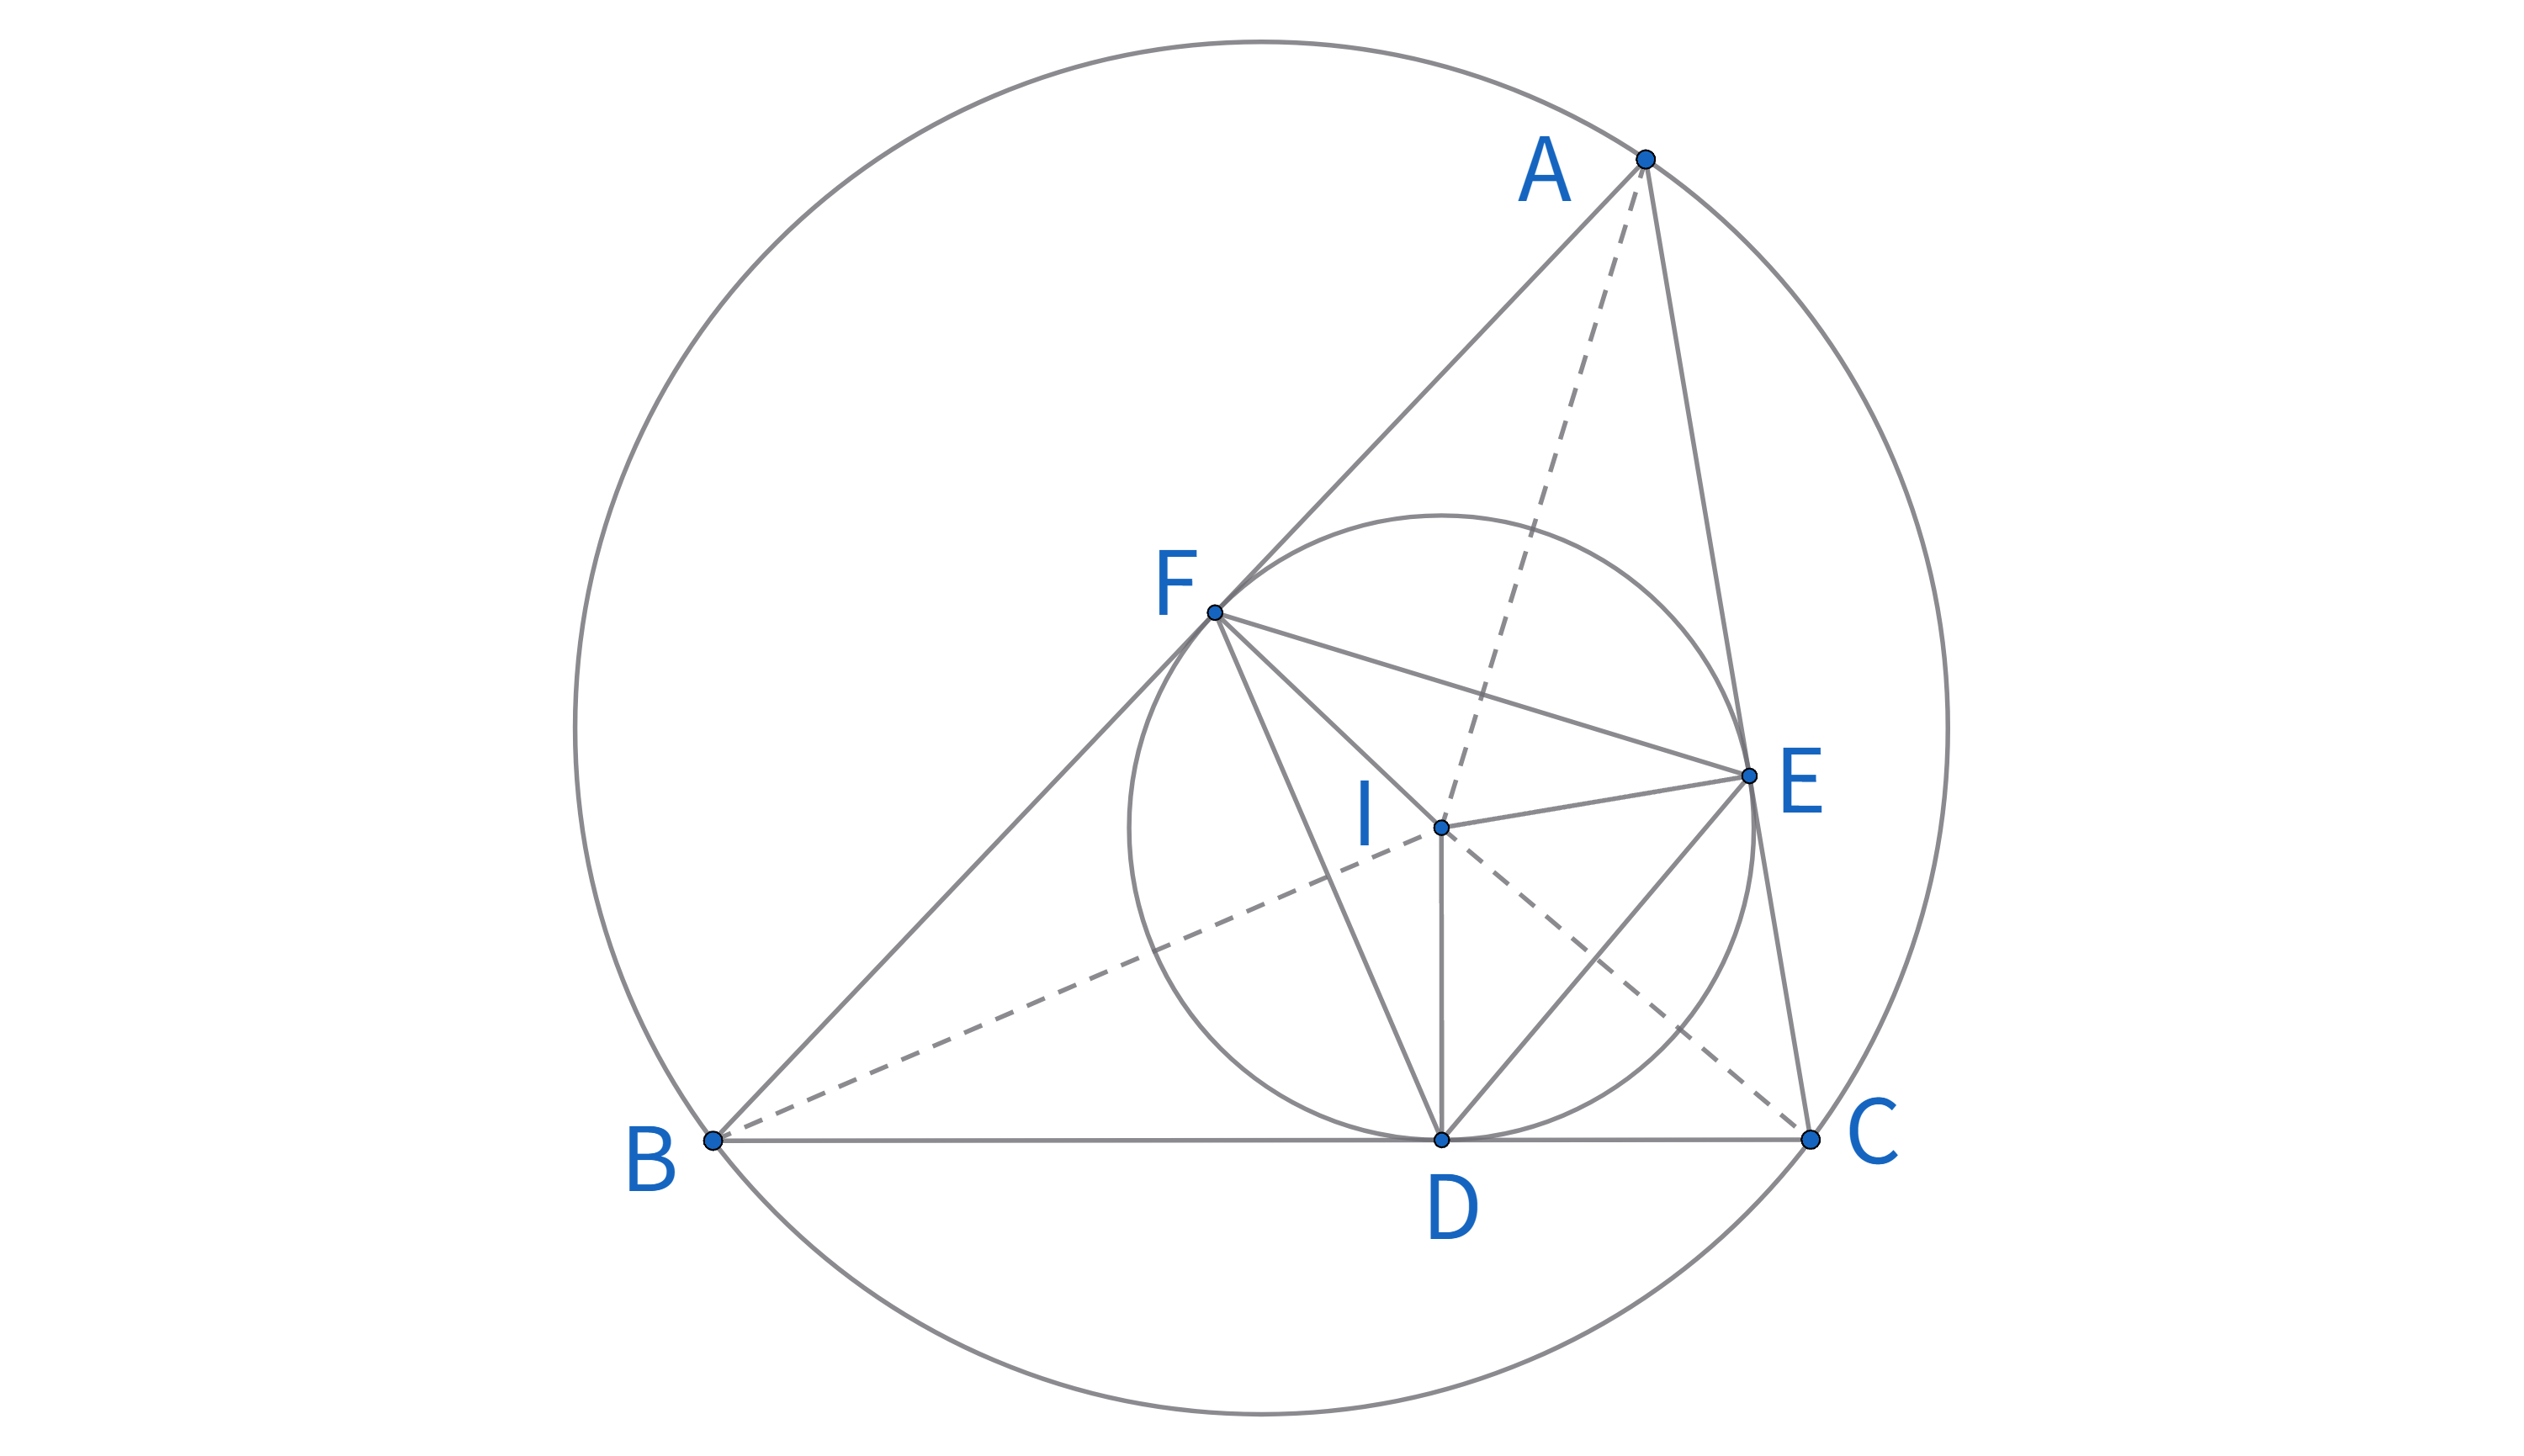
\includegraphics[width=0.7\linewidth]{figures/三角形五心/切点三角形.png}
%     \caption{切点三角形}
% \end{figure}


%--------------------------------------------------------------
\newpage
\section{垂心}
\begin{definition}[垂心]
    三角形三边上高线的交点称为三角形的垂心,通常使用H表示。
\end{definition}

\begin{figure}[H]
    \centering
    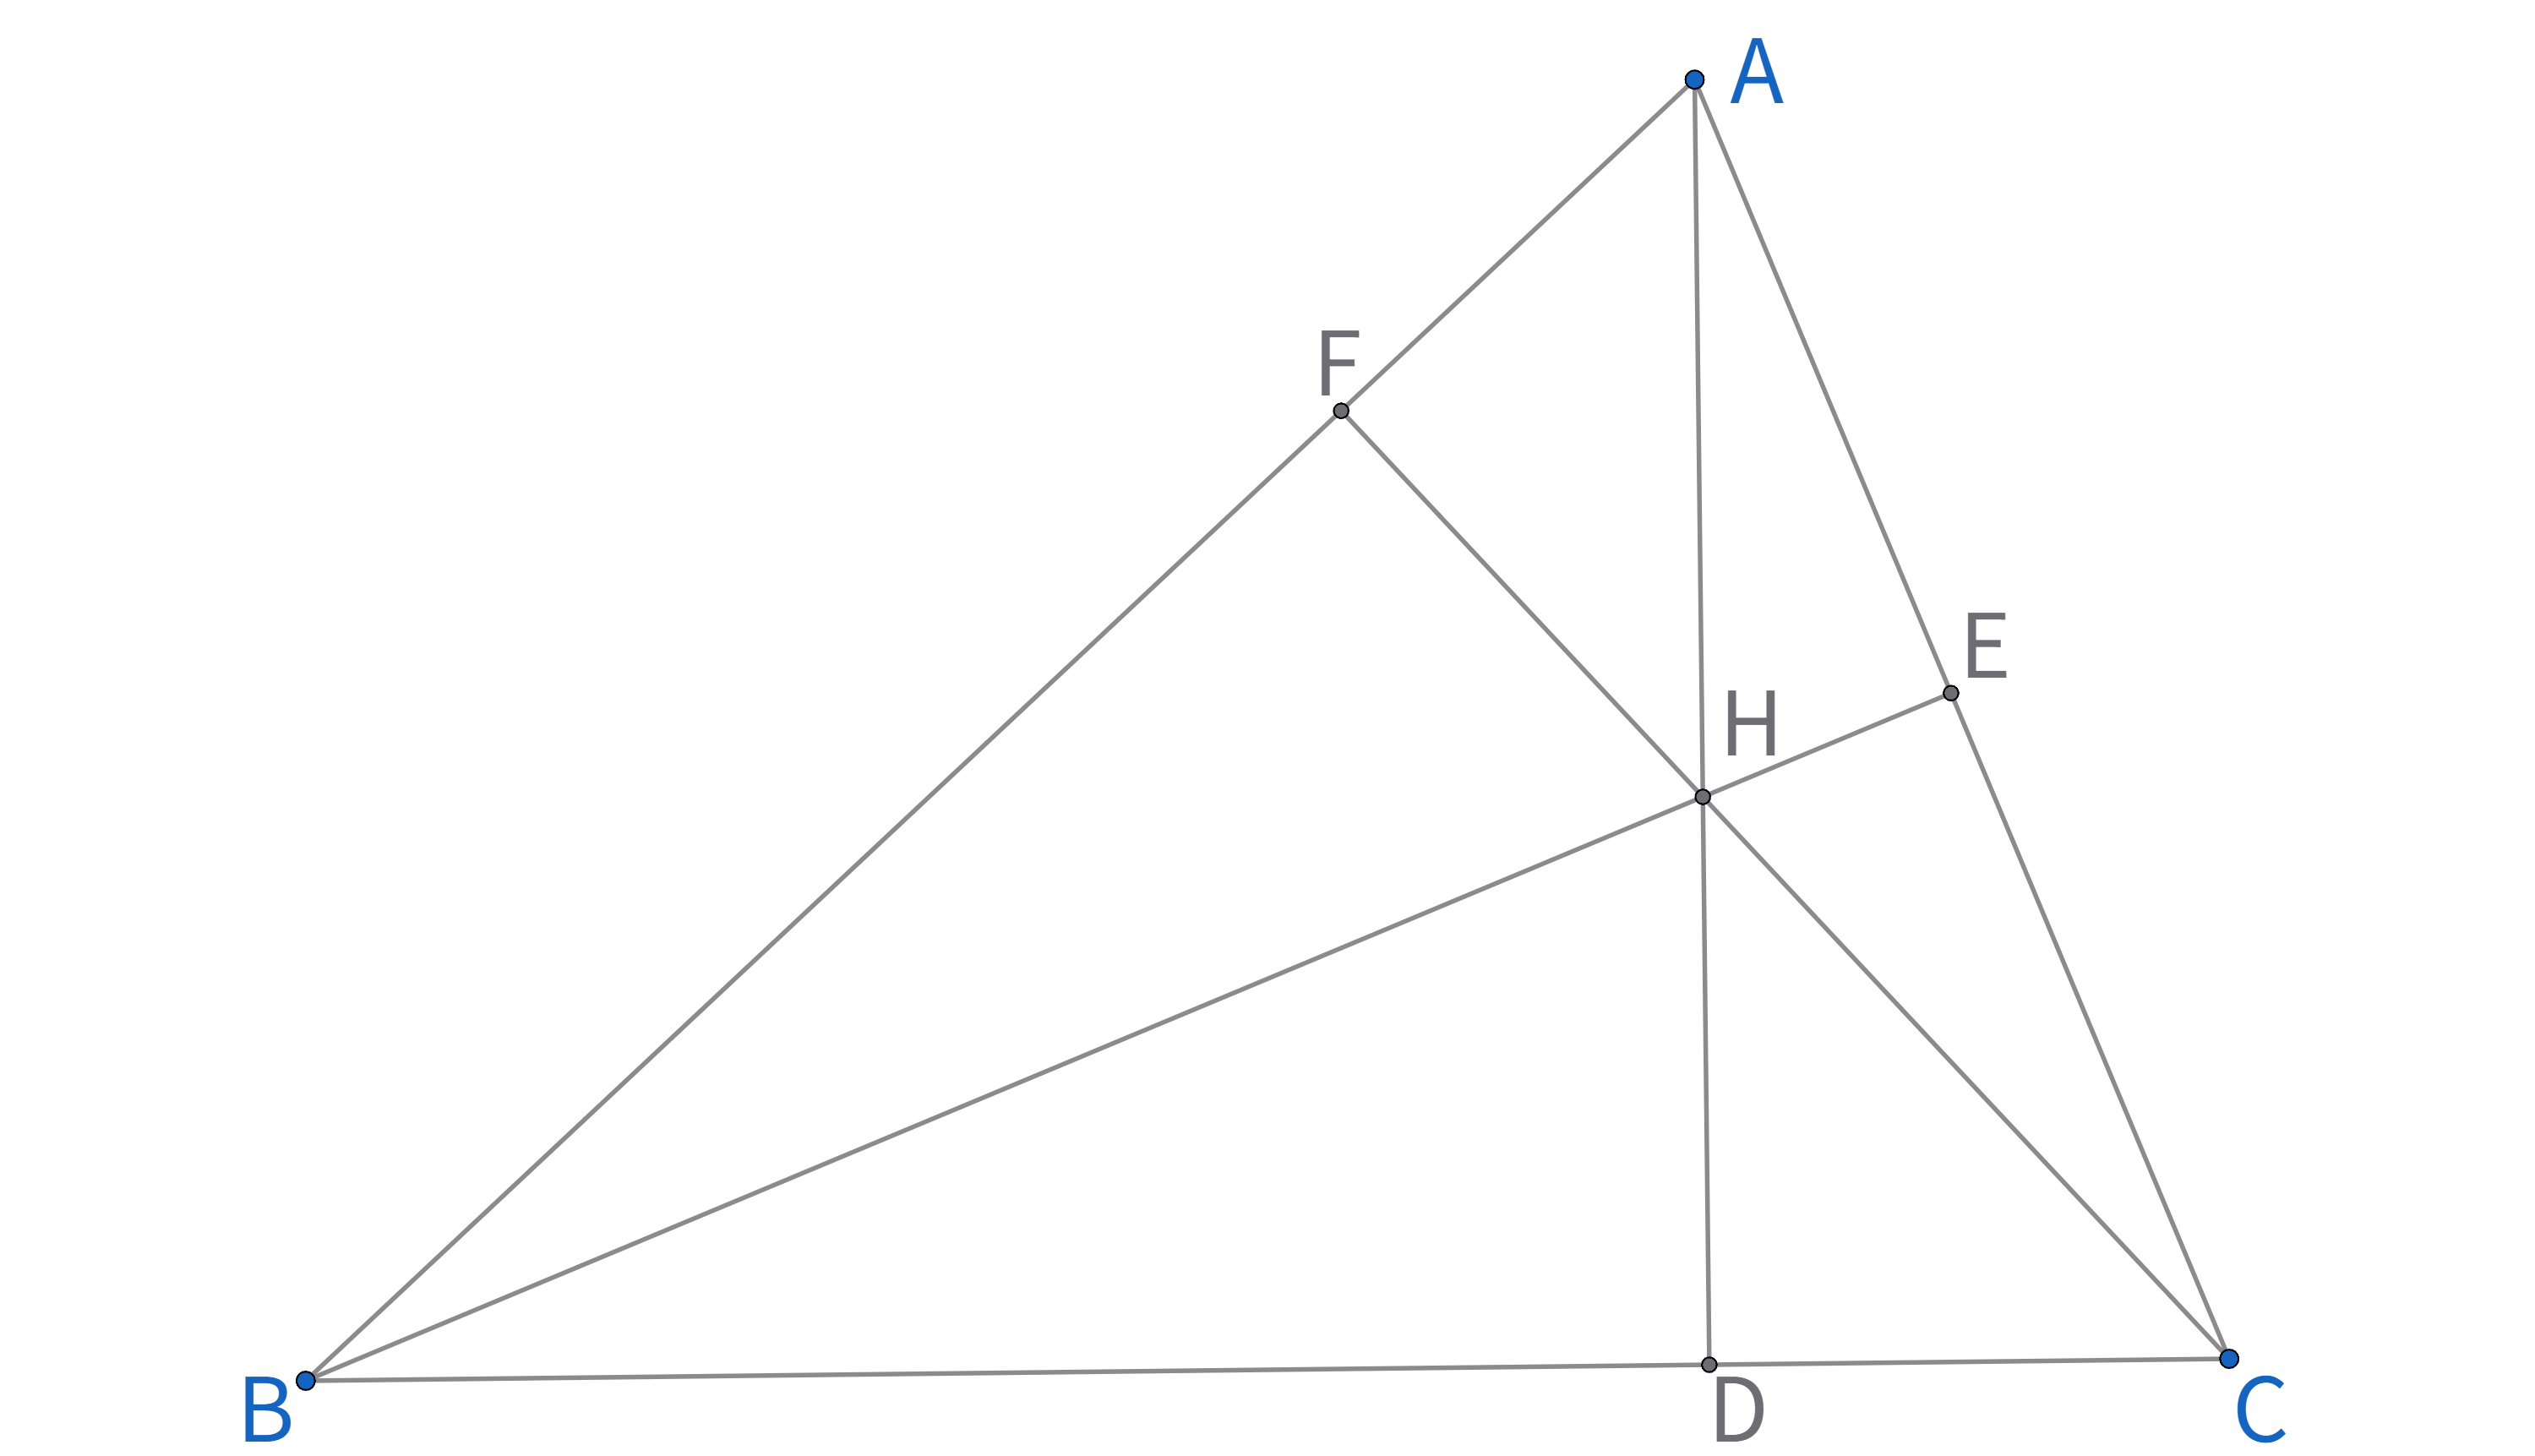
\includegraphics[width=0.8\linewidth]{figures/三角形五心/垂心.png}
    \caption{垂心}
\end{figure}

\begin{proposition}[垂心性质]
    三角形垂心具有如下性质。

    (1) 若H是三角形$\triangle ABC$的垂心,则
    $$\angle BHC = 180^\circ - A,\quad \angle AHC = 180^\circ - B,\quad \angle AHB =180^\circ - C.$$

    (2) 设$\triangle ABC$的外接圆半径为R,则
    $$AH=2R\cdot |\cos A|,\quad
    BH=2R\cdot |\cos B|,\quad
    CH=2R\cdot |\cos C|.$$

    (3) 锐角三角形的垂心在形内,直角三角形的垂心在直角顶点,钝角三角形的垂心在形外。

    (4) 若H为三角形$\triangle ABC$的垂心,则A、B、C、H四点中任意一点是其余三点构成的三角形的垂心,称A、B、C、H为垂心组。
\end{proposition}


\newpage
\subsection{垂足三角形}
\begin{proposition}[垂足三角形]
    设$\triangle DEF$ 是锐角$\triangle ABC$的垂足三角形,H是垂心,则:
    (1) $A, E, F, H$在以$AH$为直径的圆上。

    (2) $B, E, F, C$在以$BC$为直径的圆上。

    (3) $H$ 是 $\triangle DEF$的内心。
\end{proposition}
\begin{figure}[H]
    \centering
    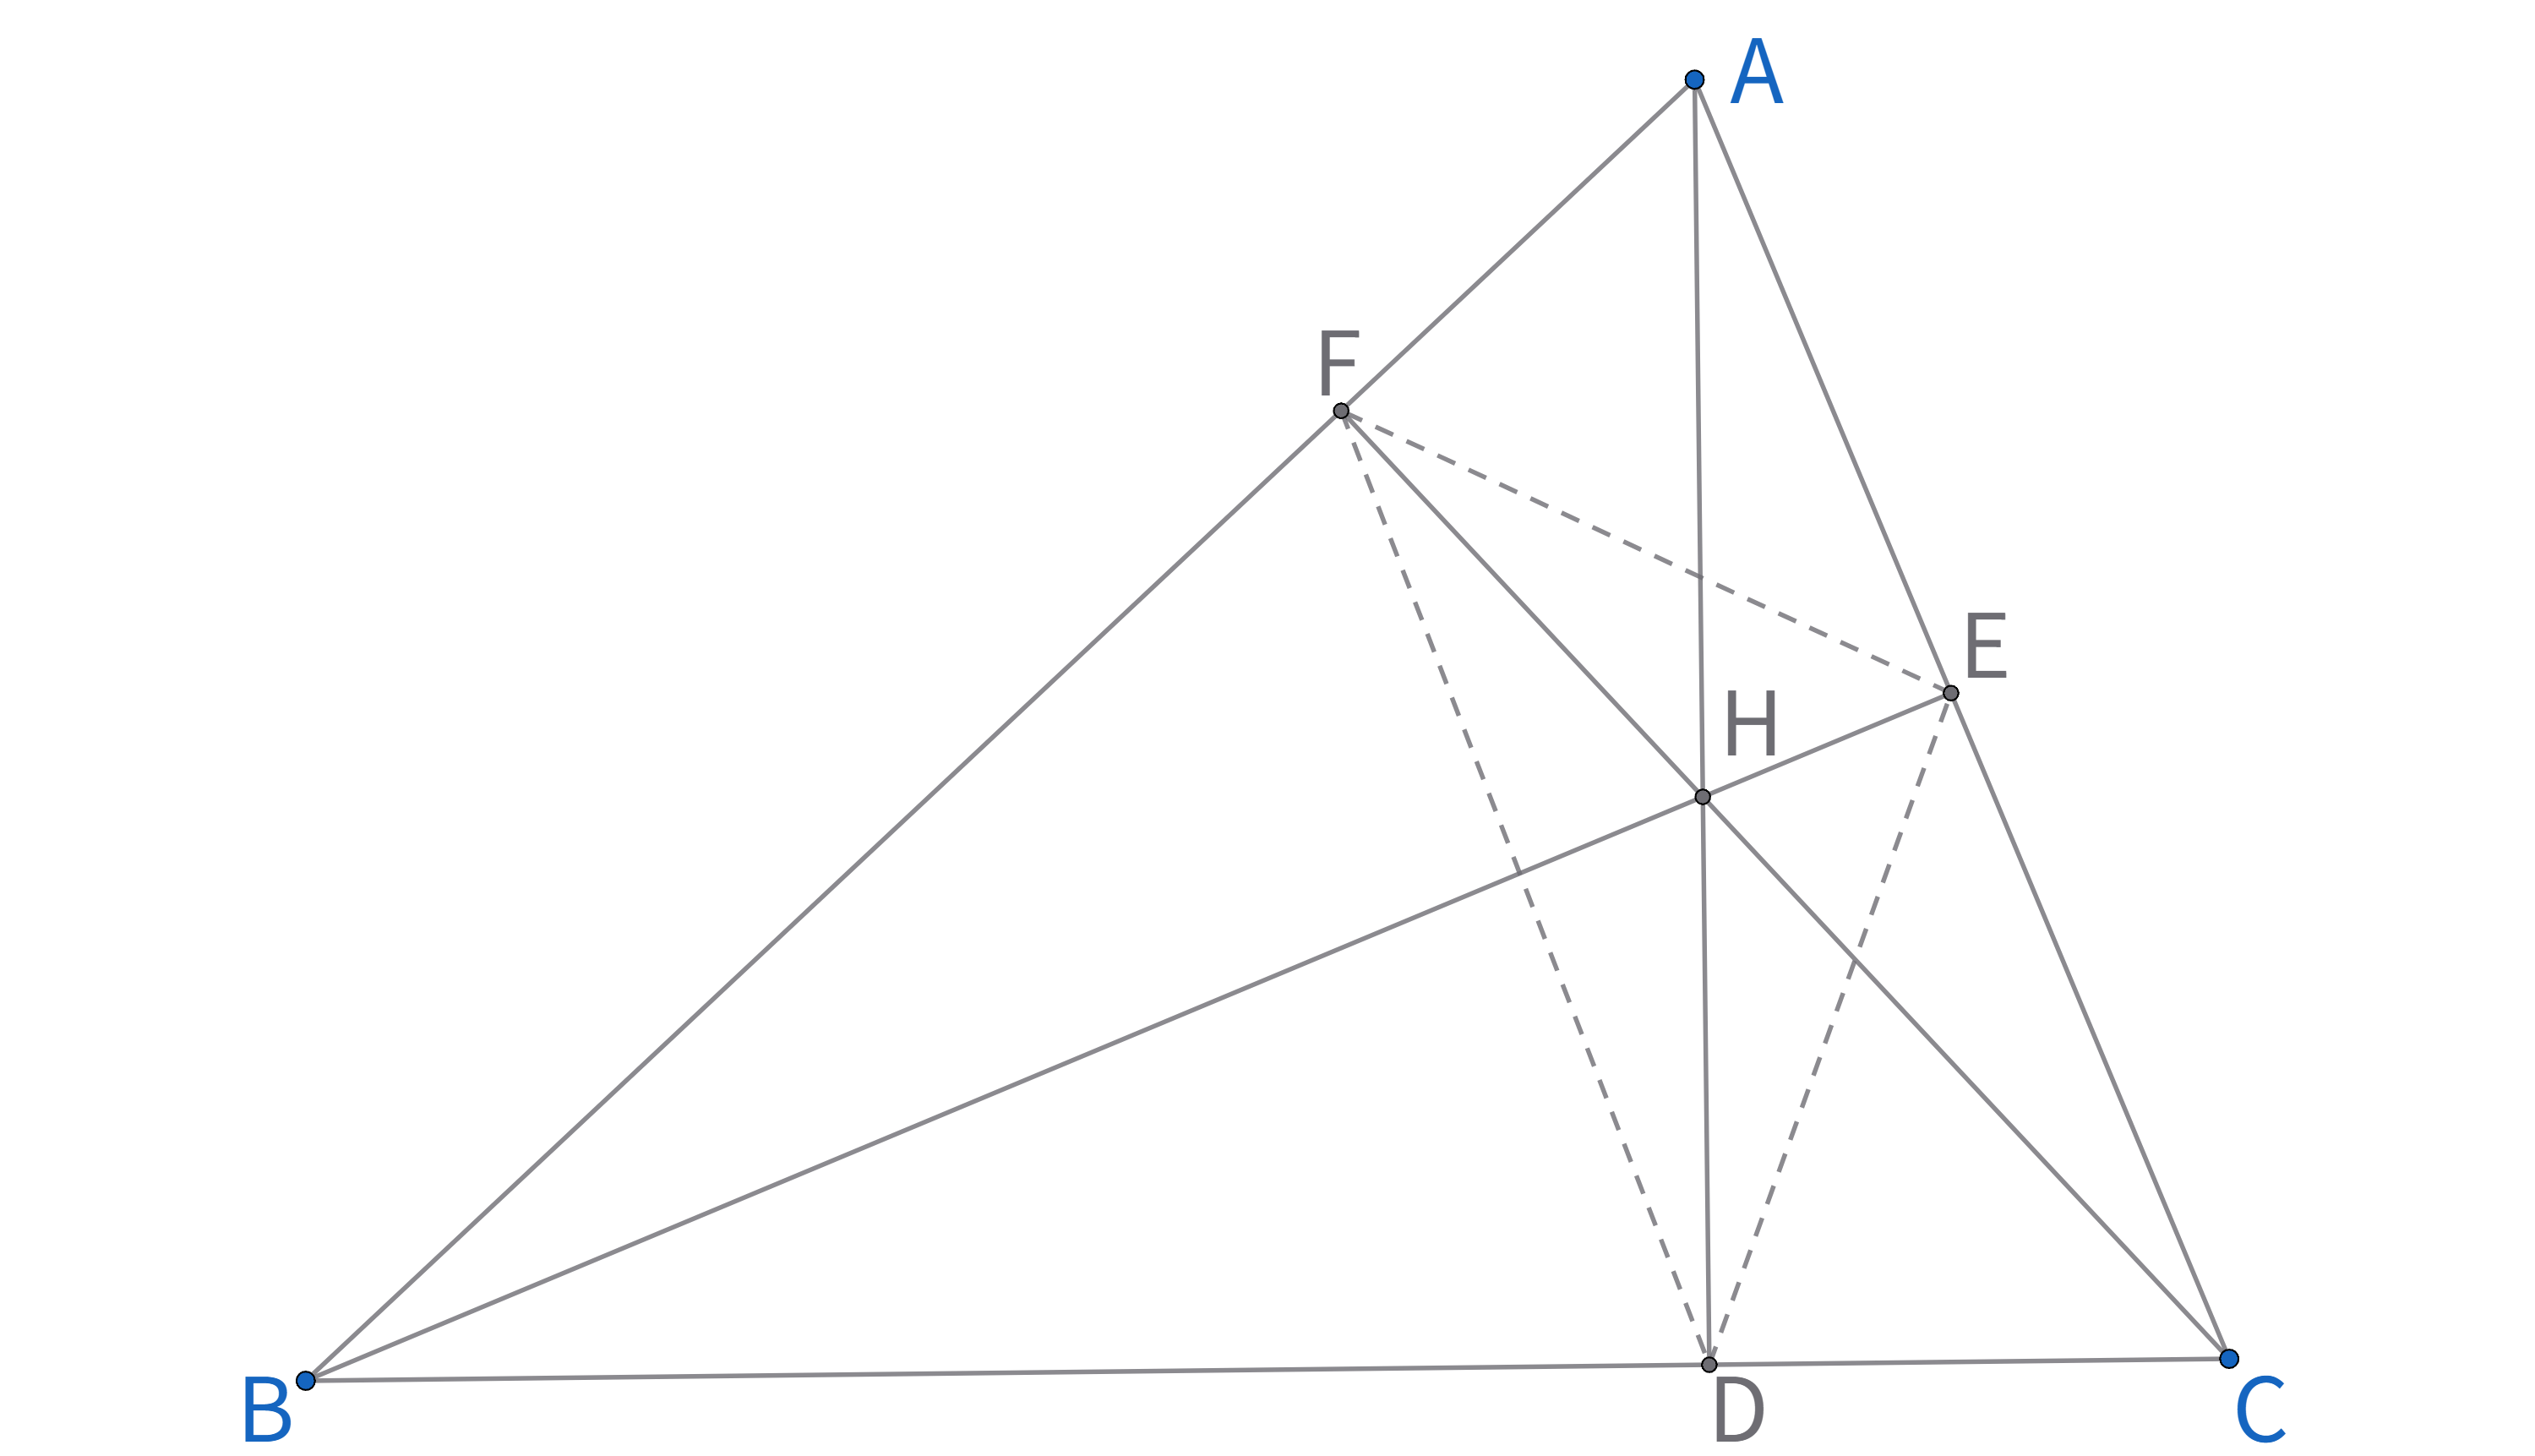
\includegraphics[width=0.8\linewidth]{figures/三角形五心/垂足三角形.png}
    \caption{垂足三角形}
\end{figure}

\begin{exercise}
    用$\triangle ABC$的三边边长,以及三顶角的三角函数表示下面的量。

    (1) 顶点与垂足连线段的长度,如$BD, CD$。

    (2) 垂心$H$到三边的距离,如$HD$。

    (3) 垂心$H$到三顶点的距离,如$HA$。

    (4) 两垂足连线段的长度,如$EF$。

    (5) 计算图中所有角的度数,如$\angle BAH, \angle AHF, \angle AEF, \angle FHE$。  
\end{exercise}




\newpage 
\subsection{垂心的对称性质}
\begin{figure}[H]
    \centering
    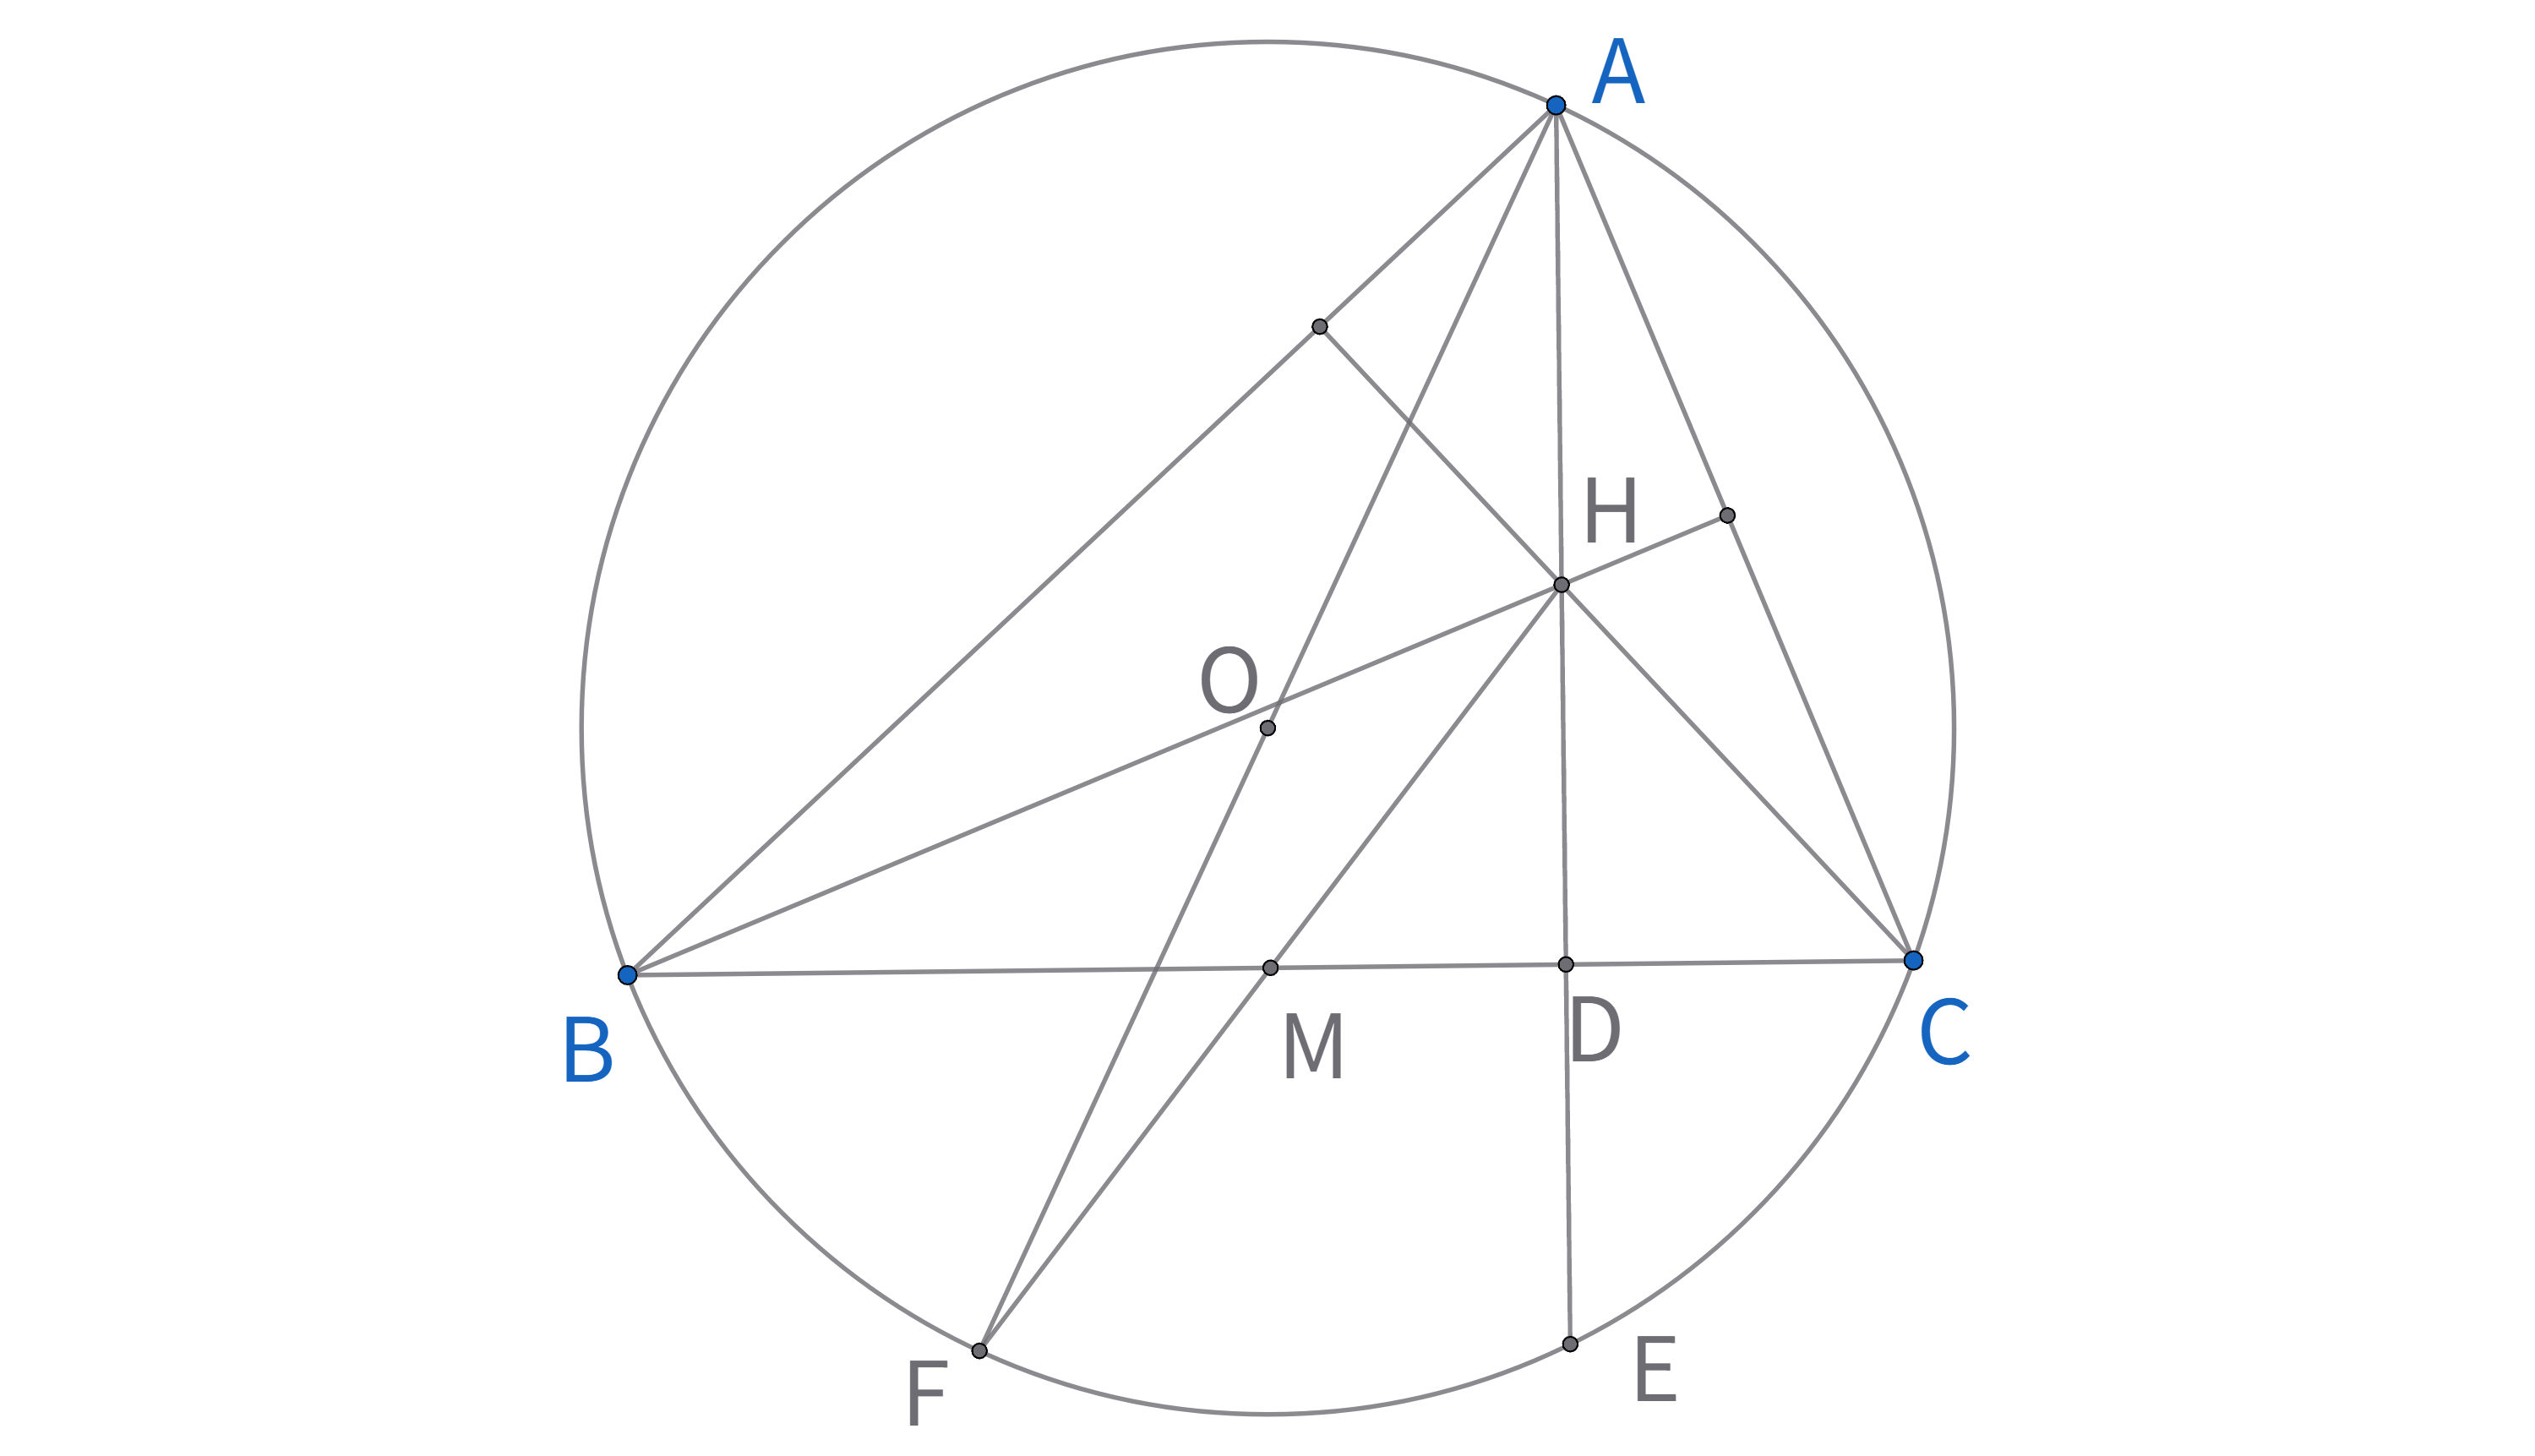
\includegraphics[width=0.8\linewidth]{figures/三角形五心/垂心的对称性质.png}
    \caption{垂心性质}
\end{figure}

\begin{theorem}[垂心的对称性质]
    设$H$是$\triangle ABC$的垂心,设$E$ 是 $H$ 关于$BC$的对称点, $F$ 是$H$ 关于 $BC$中点$M$的对称点。

    (1) $E$在$\triangle ABC$的外接圆$O$上。


    (2) $F$在$\triangle ABC$的外接圆$O$上。

    (3) $A, O, F$ 三点共线。

    (4) (卡诺定理) 顶点到垂心距离是外心到对边距离的2倍,即$AH = 2OM.$
   
    (5) H是外心O关于$\triangle ABC$的等角共轭点,即
    $$\angle BAO = \angle CAH, \quad 
    \angle ACO = \angle BCH, \quad 
    \angle CBO = \angle ABH.$$
\end{theorem}

% \begin{figure}[H]
%     \centering
%     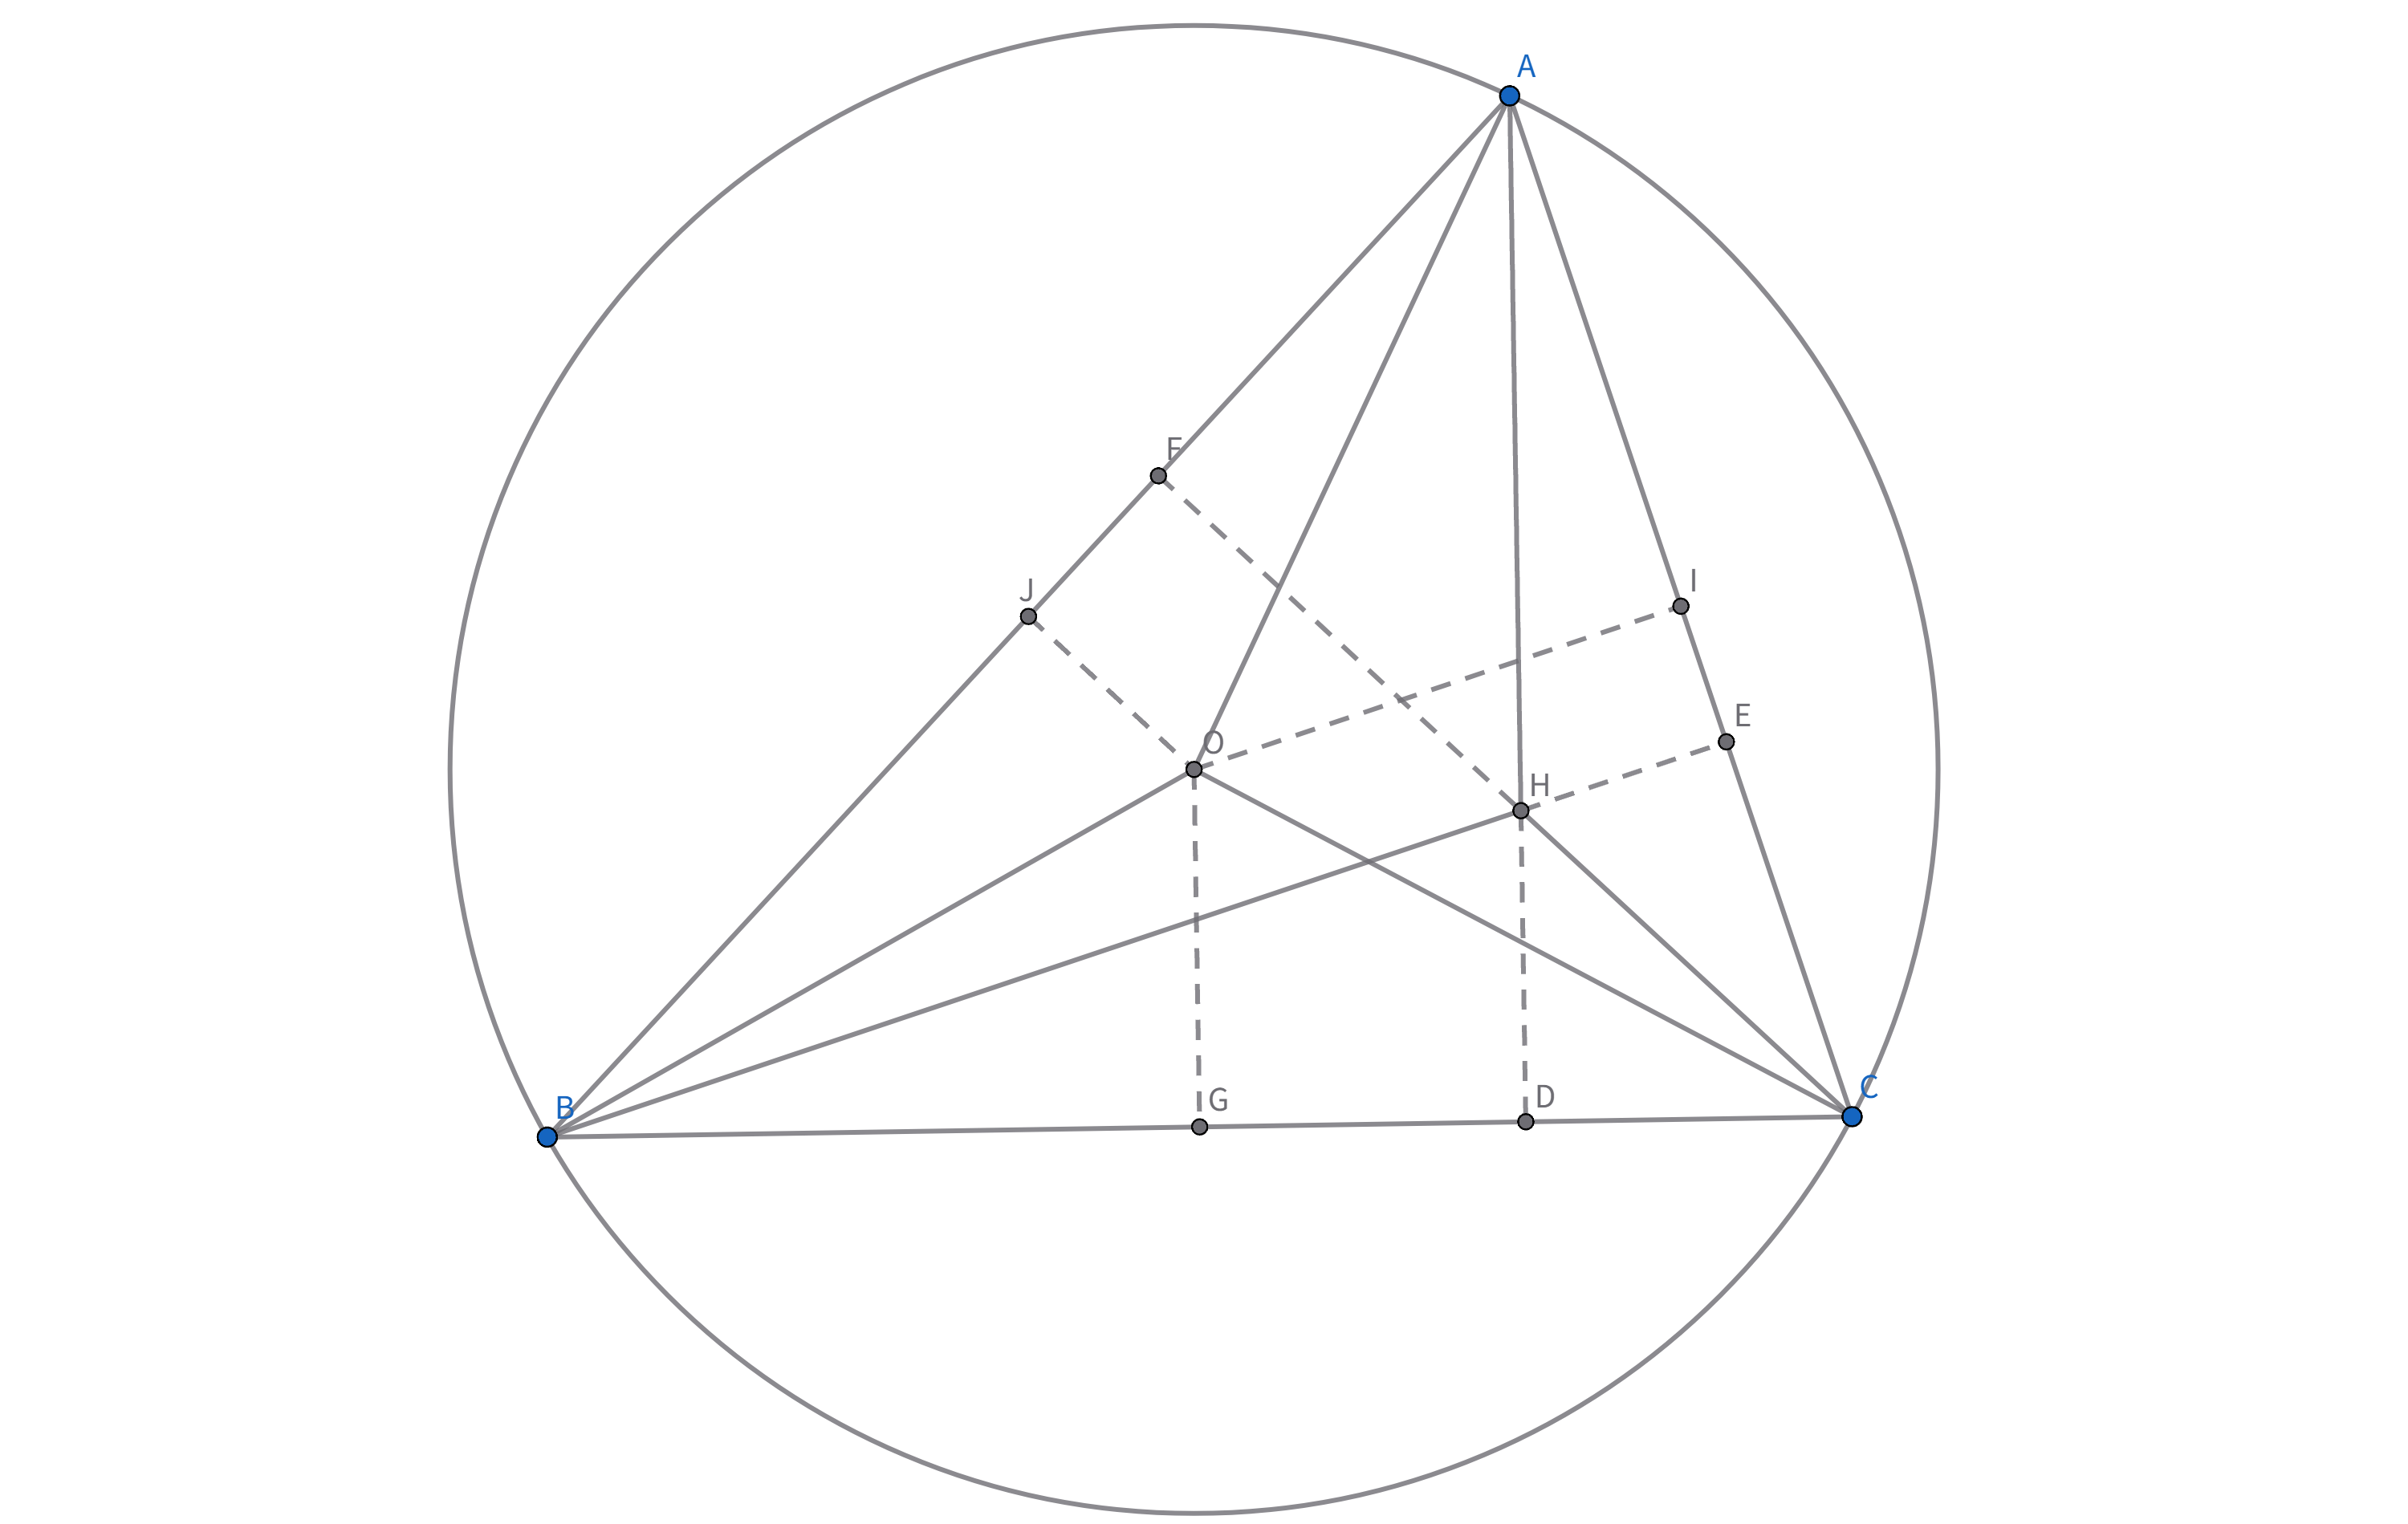
\includegraphics[width=0.5\linewidth]{figures/三角形五心/外心垂心等角共轭.png}
%     \caption{外心垂心等角共轭}
% \end{figure}


%-----------------------------------------------------------------------------------------
\newpage
\section{重心}
\begin{definition}[重心]
    三角形三条中线的交点称为三角形的重心,通常使用G表示。
\end{definition}

\begin{figure}[H]
    \centering
    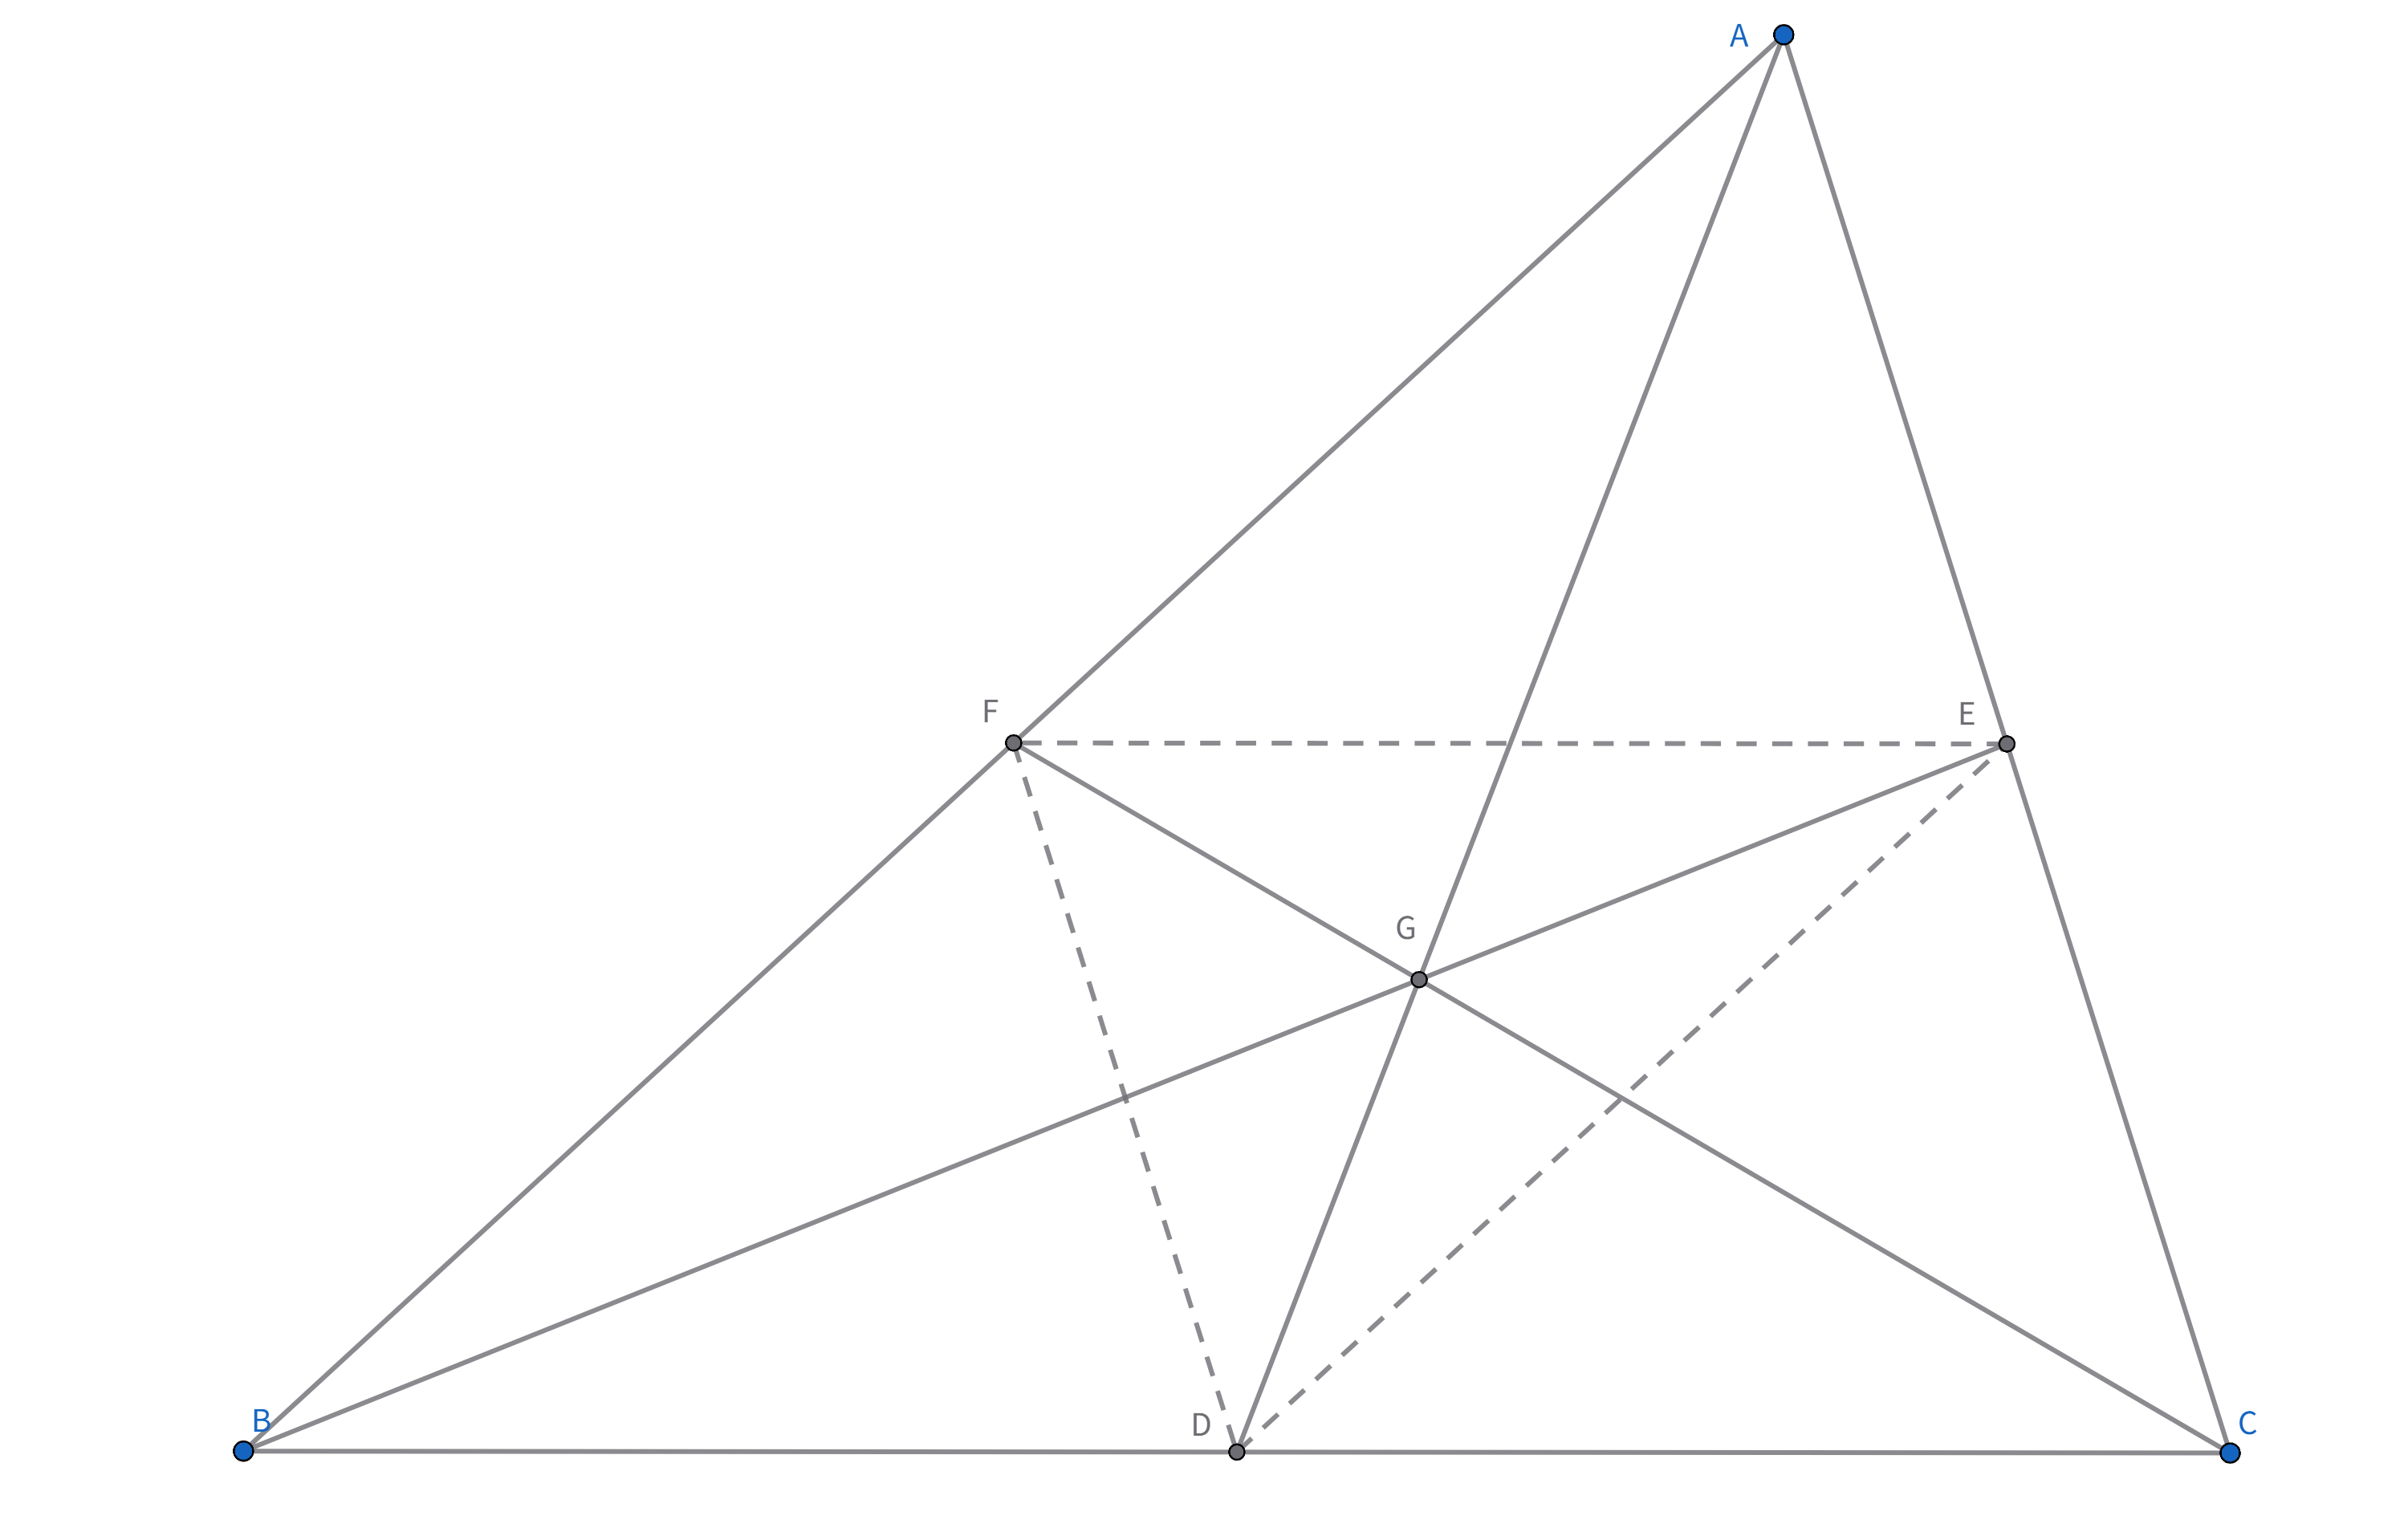
\includegraphics[width=0.8\linewidth]{figures/重心.png}
    \caption{重心}
\end{figure}

\begin{proposition}[重心性质]
    三角形重心具有如下性质。
    
    (1) 重心G为三条中线的三等分点,满足
    $$AG=2GD,\quad 
    BG=2GE,\quad
    CG=2GF.$$

    (2) 三边与重心组成的三角形面积相等,即
    $$S_{\triangle ABG} = S_{\triangle BCG}=S_{\triangle CAG}.$$

    (3) $\triangle ABC \sim \triangle DEF$,且相似比为2.
\end{proposition}
%-------------------------------------------------------------
\begin{exercise}
    证明:$2AD^2=AB^2+AC^2-\frac{1}{2}BC^2.$
\end{exercise}
\begin{exercise}
    证明:在平面直角坐标系中,重心$G$的坐标可以表示为三顶点坐标的算术平均值。
\end{exercise}


\newpage
\section{旁心}
\begin{definition}[旁心]
    与三角形一边外侧相切,又与另两边的延长线相切的圆叫做三角形的旁切圆,通常用J,或者$I_a,I_b,I_c$表示。    
\end{definition}

\begin{figure}[H]
    \centering
    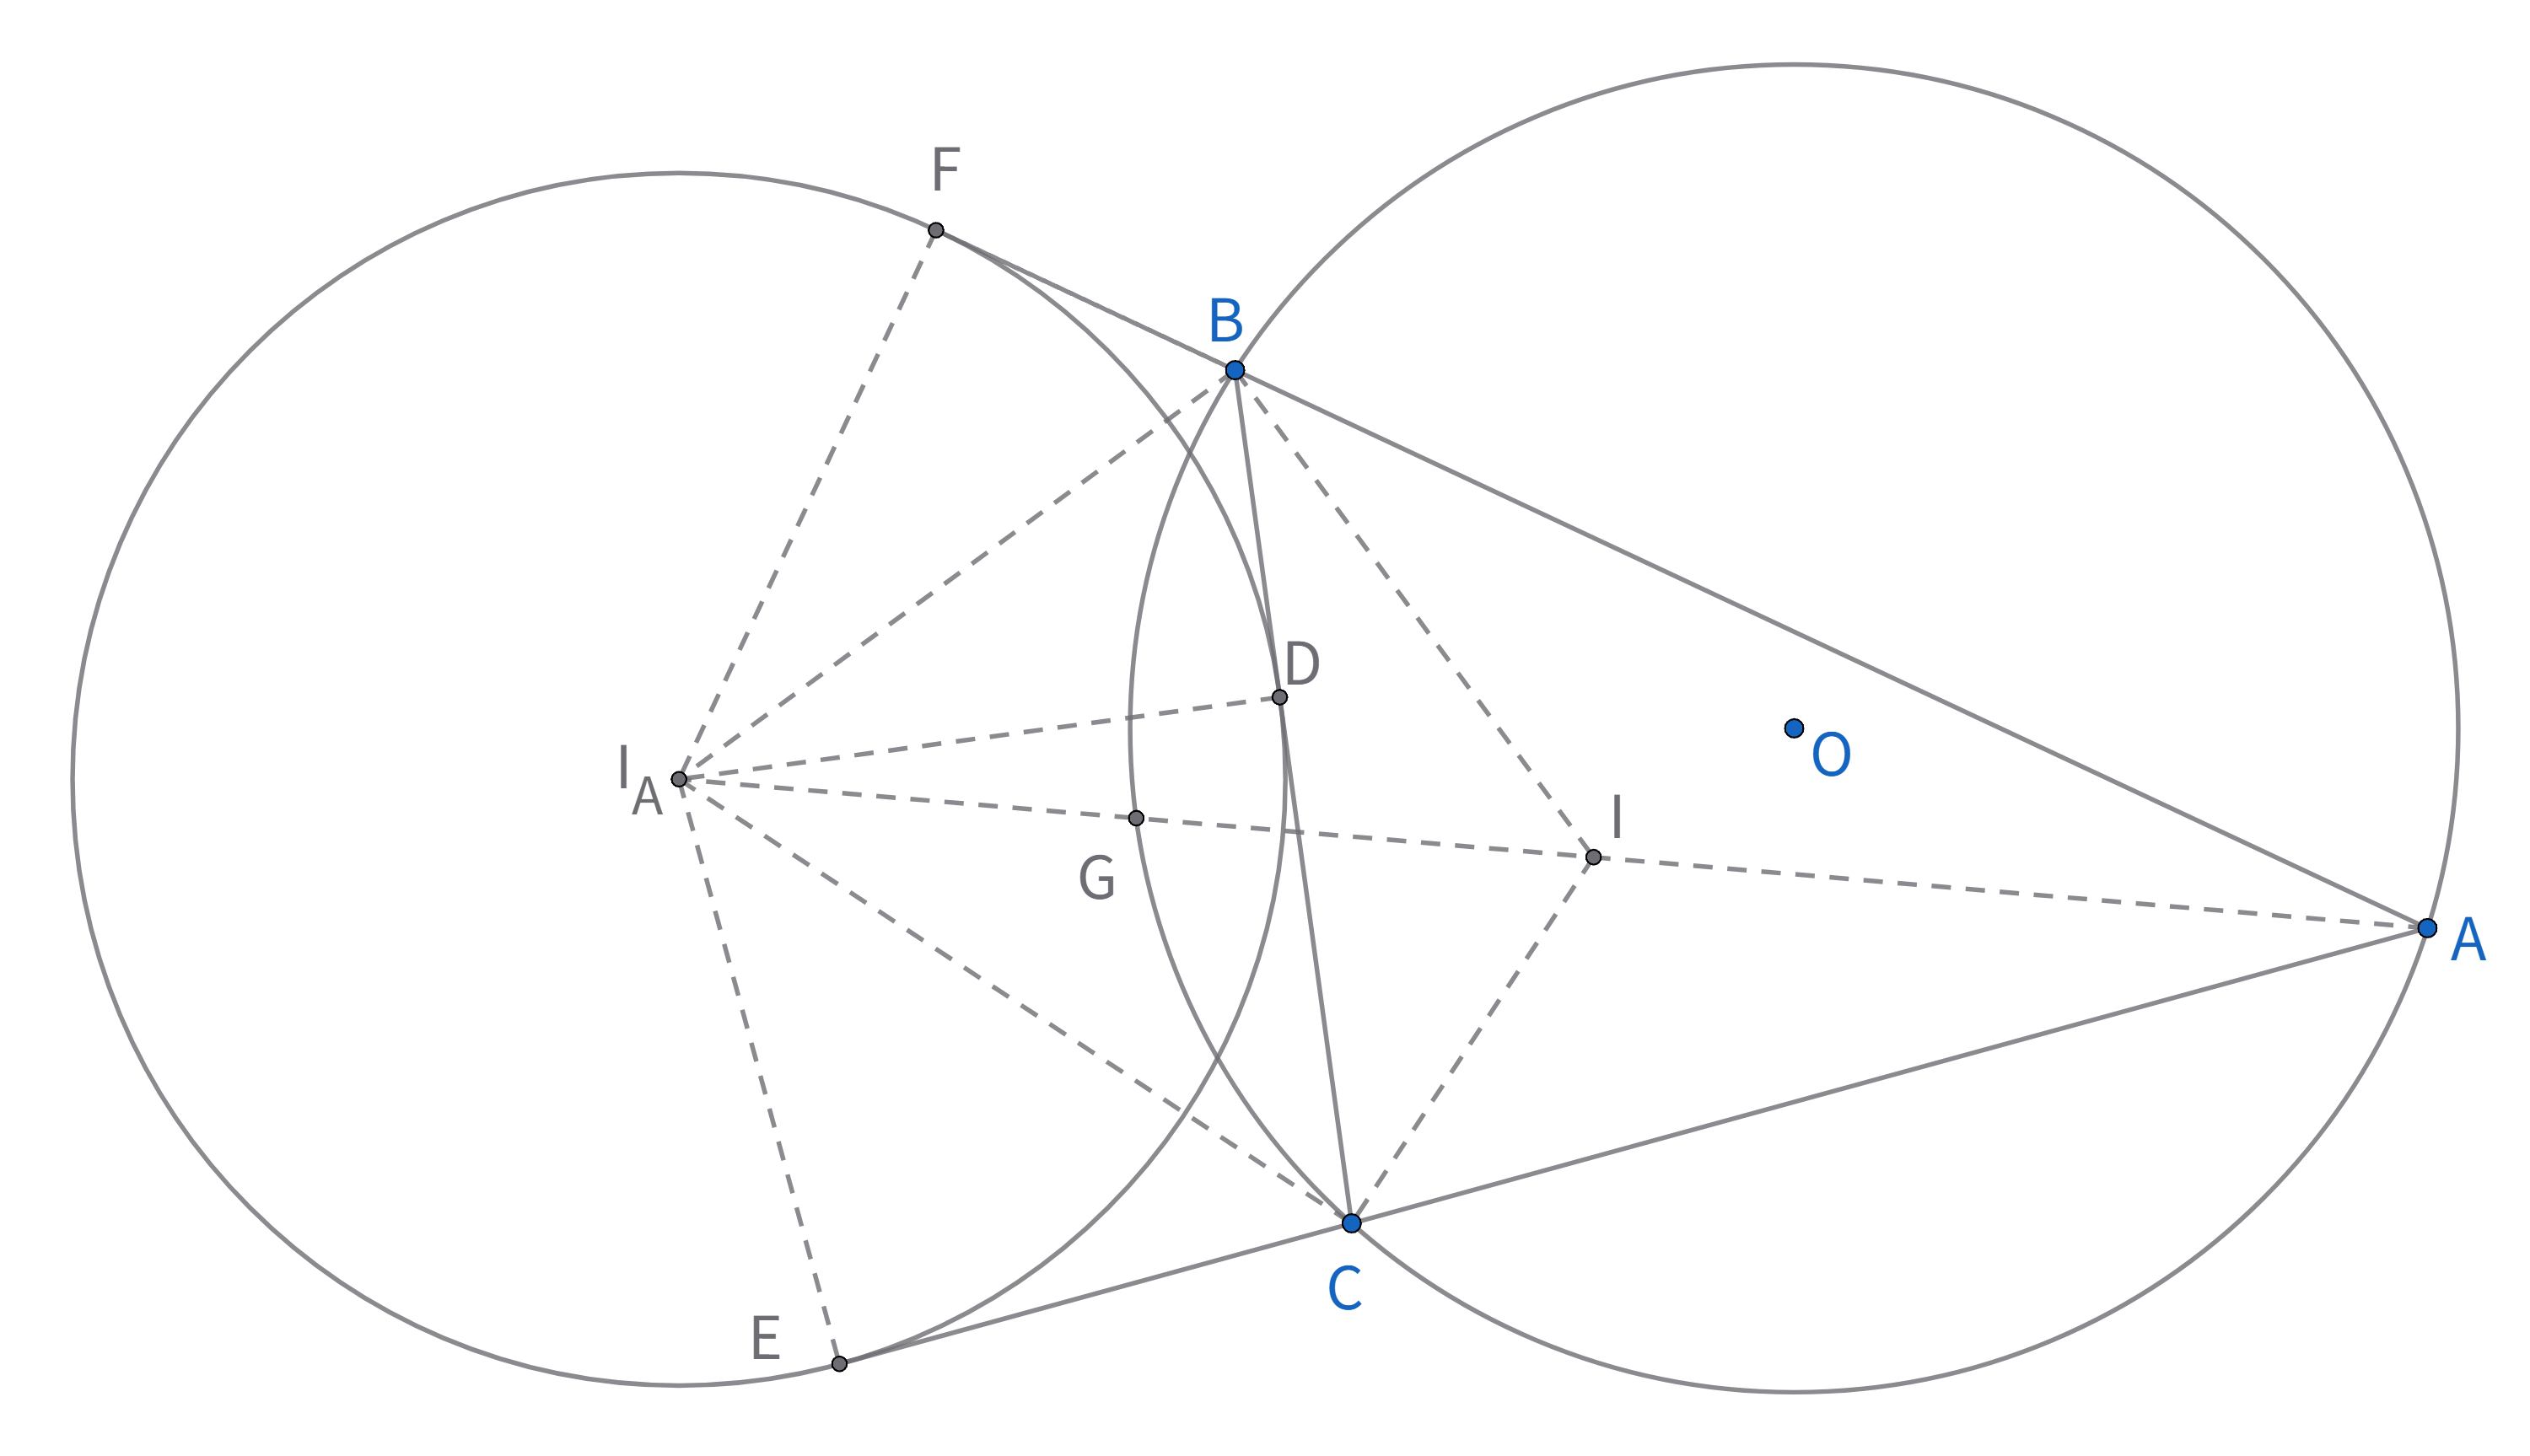
\includegraphics[width=0.6\linewidth]{figures/三角形五心/旁心.png}
    \caption{旁心}
\end{figure}


\begin{proposition}[旁心性质]
    三角形旁心具有如下性质。
    
    (1) 旁心是三角形一内角平分线及其他两角外角平分线的交点。

    (2) 旁心到三角形三边的距离相等。

    (3) $\angle I_ABC = 90^\circ - \frac{1}{2}B, \angle I_ACB = 90^\circ - \frac{1}{2}C, \angle BI_AC=90 - \frac{1}{2}A.$

    (4) $IB\perp BI_A, \quad IC\perp CI_A.$
\end{proposition}

\begin{proposition}[切线长性质]
    设D、E、F分别为旁切圆$I_A$在BC、CA、AB上的切点,则
    $$
    \begin{aligned}
    AE&=AF= s = \frac{1}{2}(a+b+c),\\
    BF&=BD=s - c =\frac{1}{2}(a+b-c),\\
    CD&=CE=s - b= \frac{1}{2}(a+c-b).
    \end{aligned}
    $$
\end{proposition}


\newpage 
\subsection{鸡爪定理}
\begin{theorem}[鸡爪定理]
    对平面内任意$\triangle ABC$,$I,J$ 分别为其内心和A-旁心,设$AI$延长线与圆$O$相交于$D$,则D为$\overset{{\frown}}{BC}$的中点,$IJ$的中点,并且为$IBJC$外接圆的圆心。
\end{theorem}

\begin{figure}[H]
    \centering
    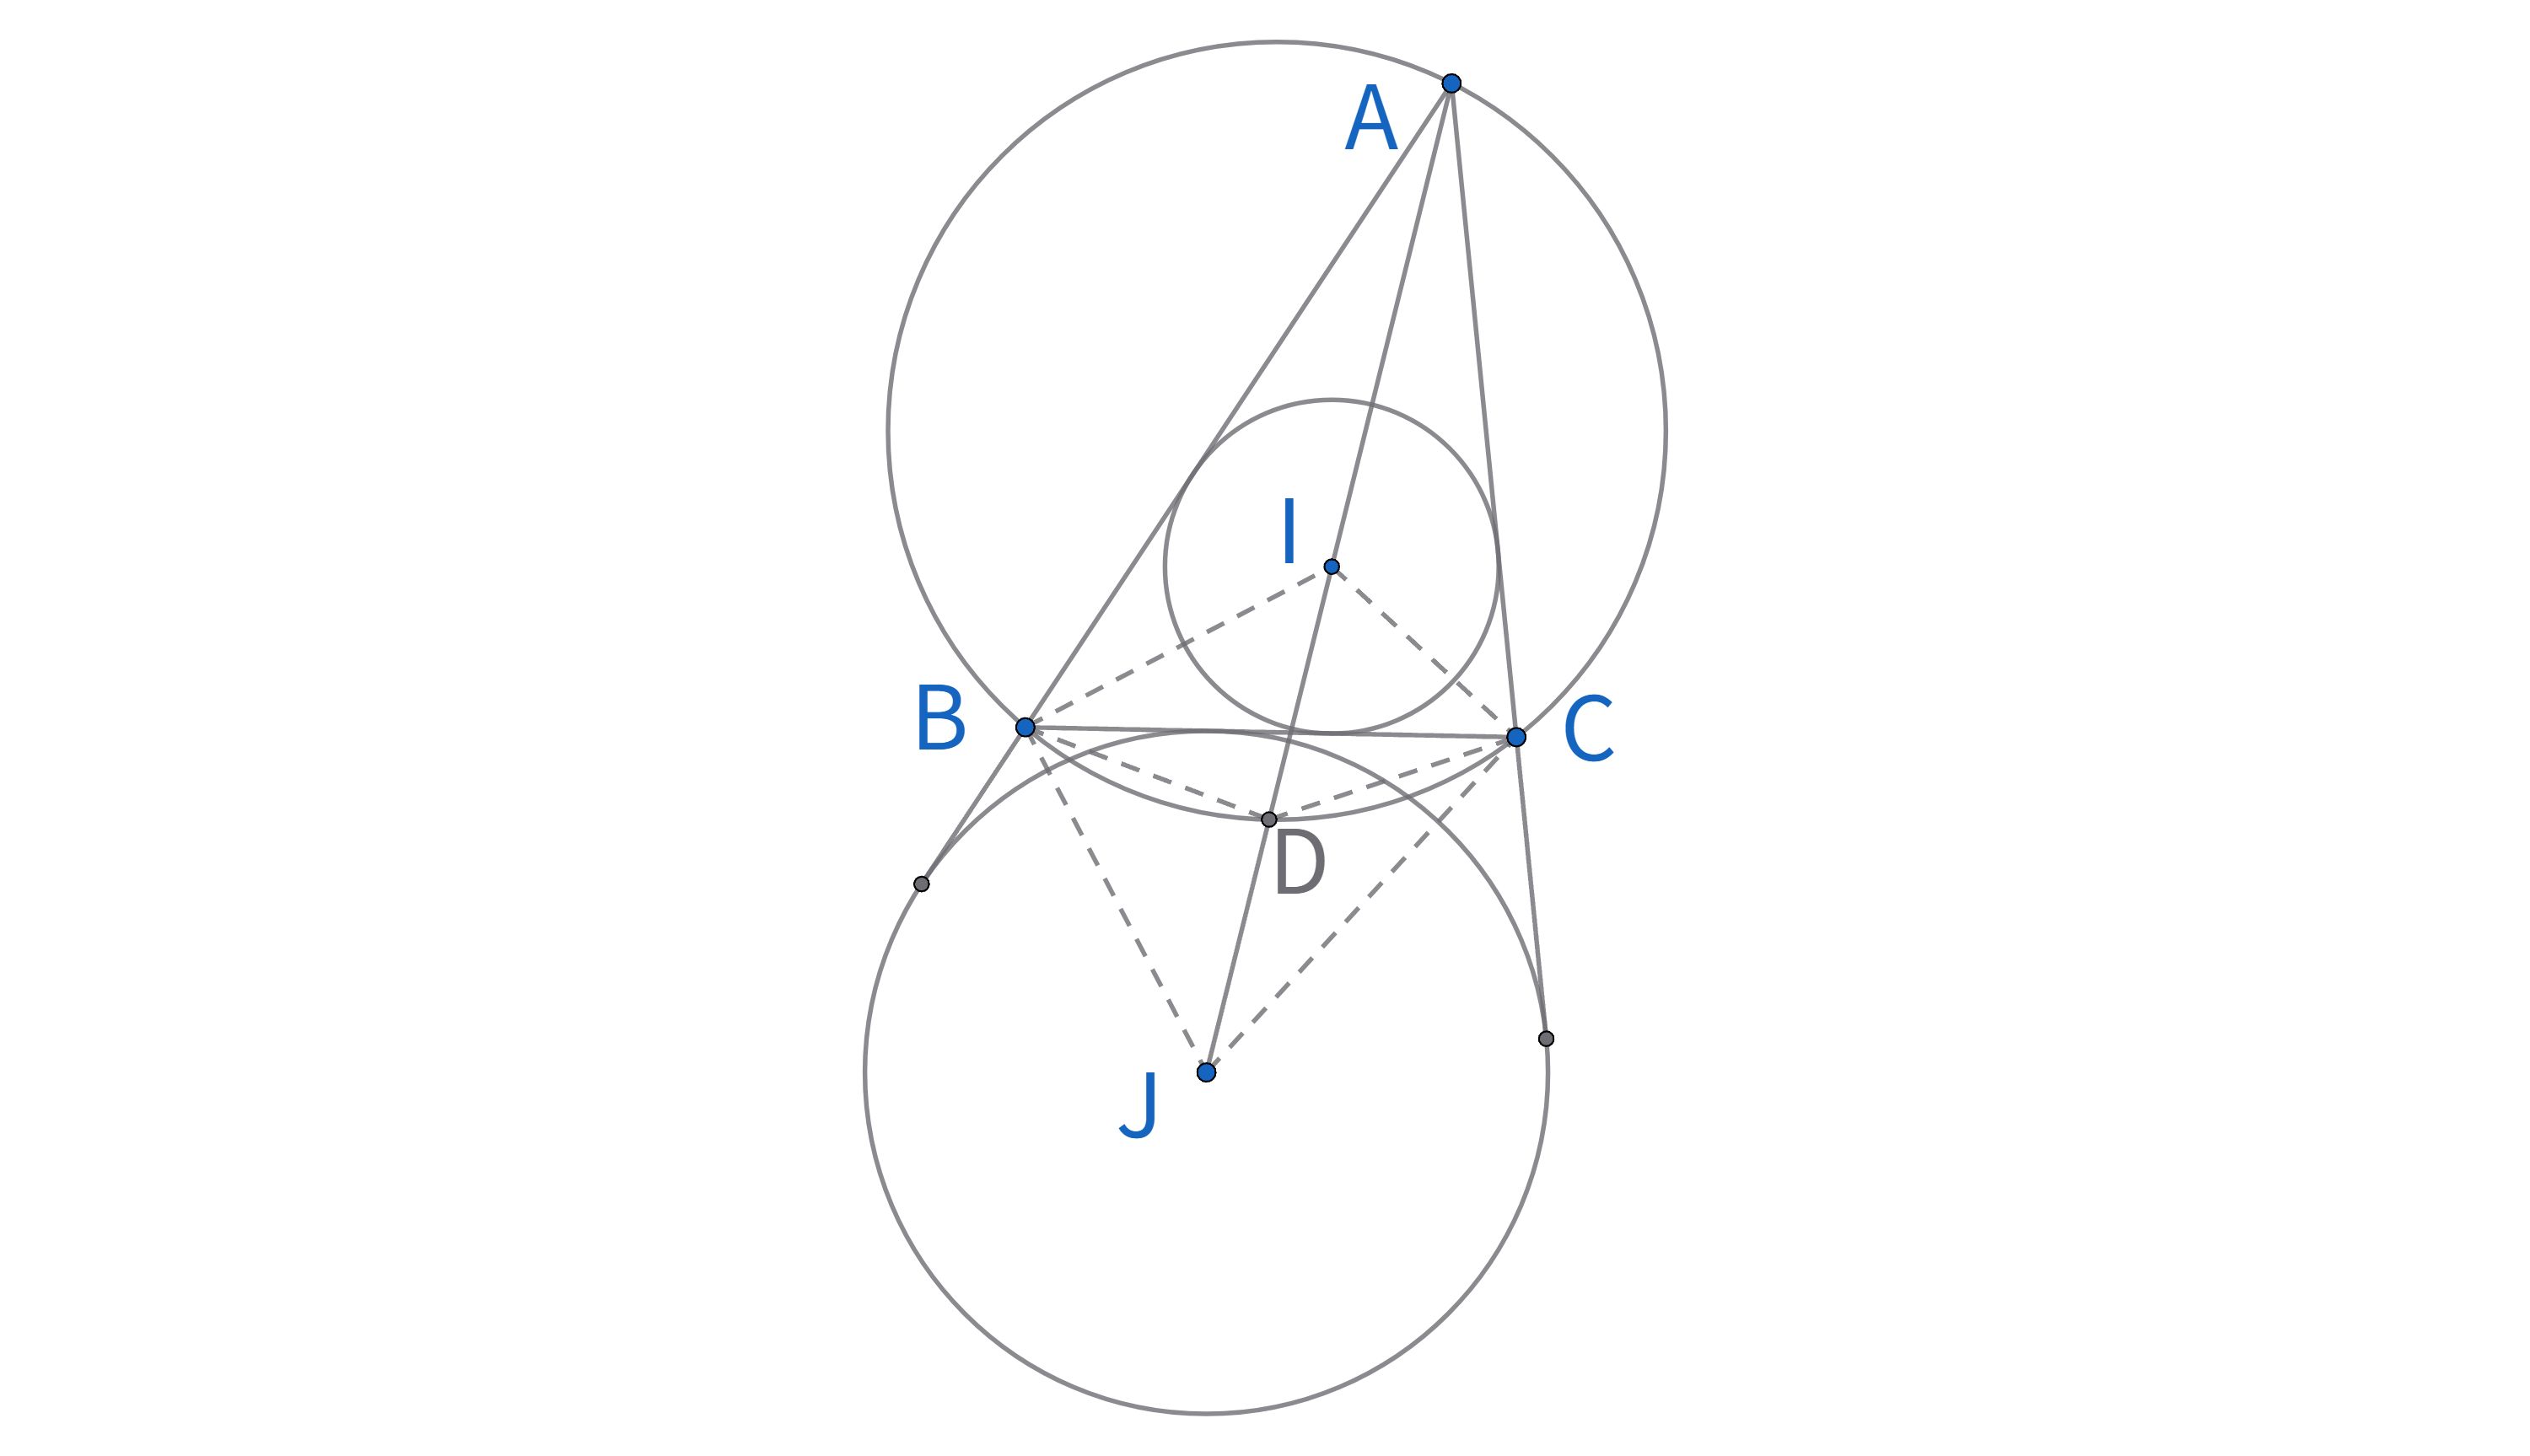
\includegraphics[width=\linewidth]{figures/三角形五心/鸡爪定理2.png}
    \caption{鸡爪定理}
\end{figure}

\begin{exercise}
    计算$\angle BIJ, \angle CIJ, \angle IBD, \angle ICD$。
\end{exercise}
\begin{exercise}
    计算$IJ$。
\end{exercise}
\begin{exercise}[旁切圆半径]
    证明:A-旁切圆的半径为$r_a = \frac{s}{s-a}r.$
\end{exercise}


\begin{exercise}
    设 $\triangle ABC$ 的内切圆和 $A$-旁切圆在 $BC$ 上的切点分别是 $D, X$。证明:$BX = CD, BD = CX$。
\end{exercise}



\newpage 
\subsection{旁心三角形}
\begin{proposition}[旁心三角形]
    对平面内任意$\triangle ABC$,$I, I_A,I_B,I_C$ 为其内心和三旁心。则$I$是旁心所构成$\triangle I_AI_BI_C$ 的垂心,$\triangle ABC$是其垂足三角形。
\end{proposition}

\begin{figure}[H]
    \centering
    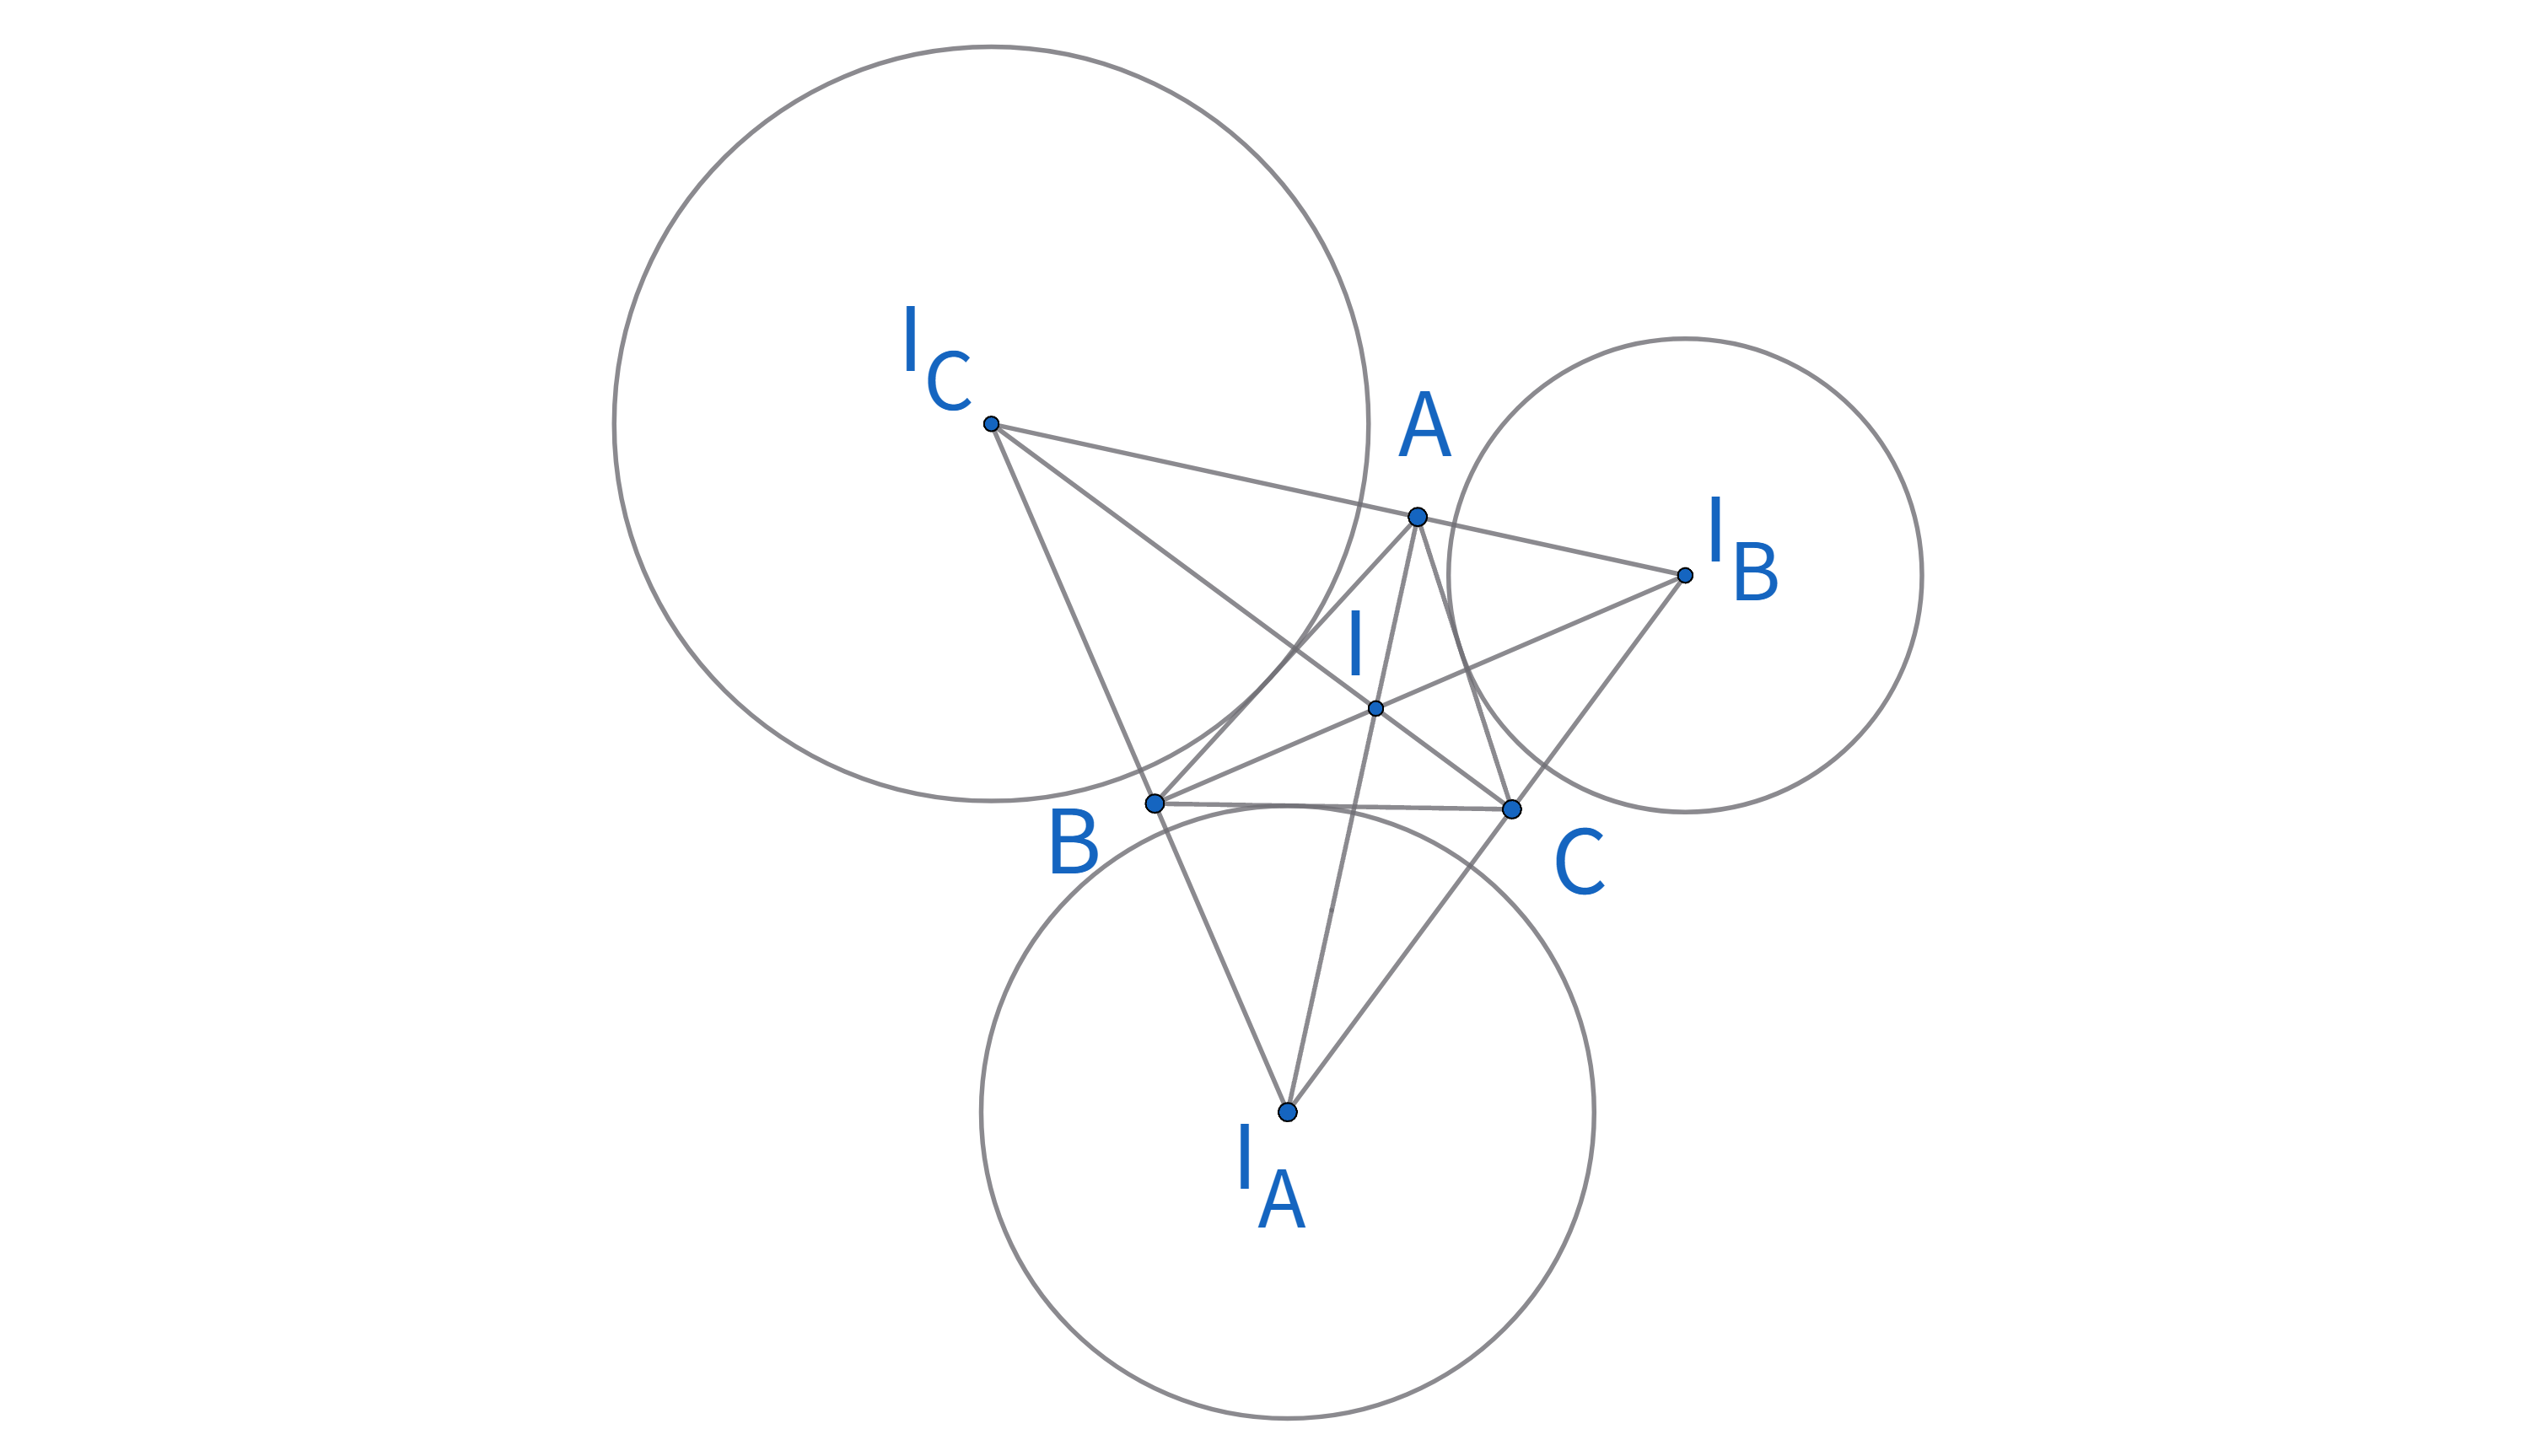
\includegraphics[width=\linewidth]{figures/三角形五心/旁心三角形.png}
    \caption{旁心三角形}
\end{figure}





% \part{圆幂与根心}
% 相交弦定理





\section{圆幂}
\begin{definition}[圆幂]
    定义$P$点到圆$O$的圆幂为
    $$\text{Pow}_O(P) = OP^2 - R^2,$$
    其中$R$为圆$O$的半径,$OP$为点$P$到圆心的距离。
\end{definition}


% 圆幂定理
\begin{theorem}[圆幂定理]
    假设平面内有一半径为R的圆O,P为平面内任意一点。
    
    (1) $\text{Pow}_O(P)$根据$P$在圆外,圆上或圆内分别取正值、零、负值。

    (2) 若直线$l$经过点$P$,与圆$O$相交于两点$A$和$B$,则
    $$PA \cdot PB = |\text{Pow}_O(P)|$$

    (3) 若$P$在圆外,$PA$与圆相切于点A,则
    $$PA^2 = |\text{Pow}_O(P)|$$
\end{theorem}
\begin{figure}[H]
    \centering
    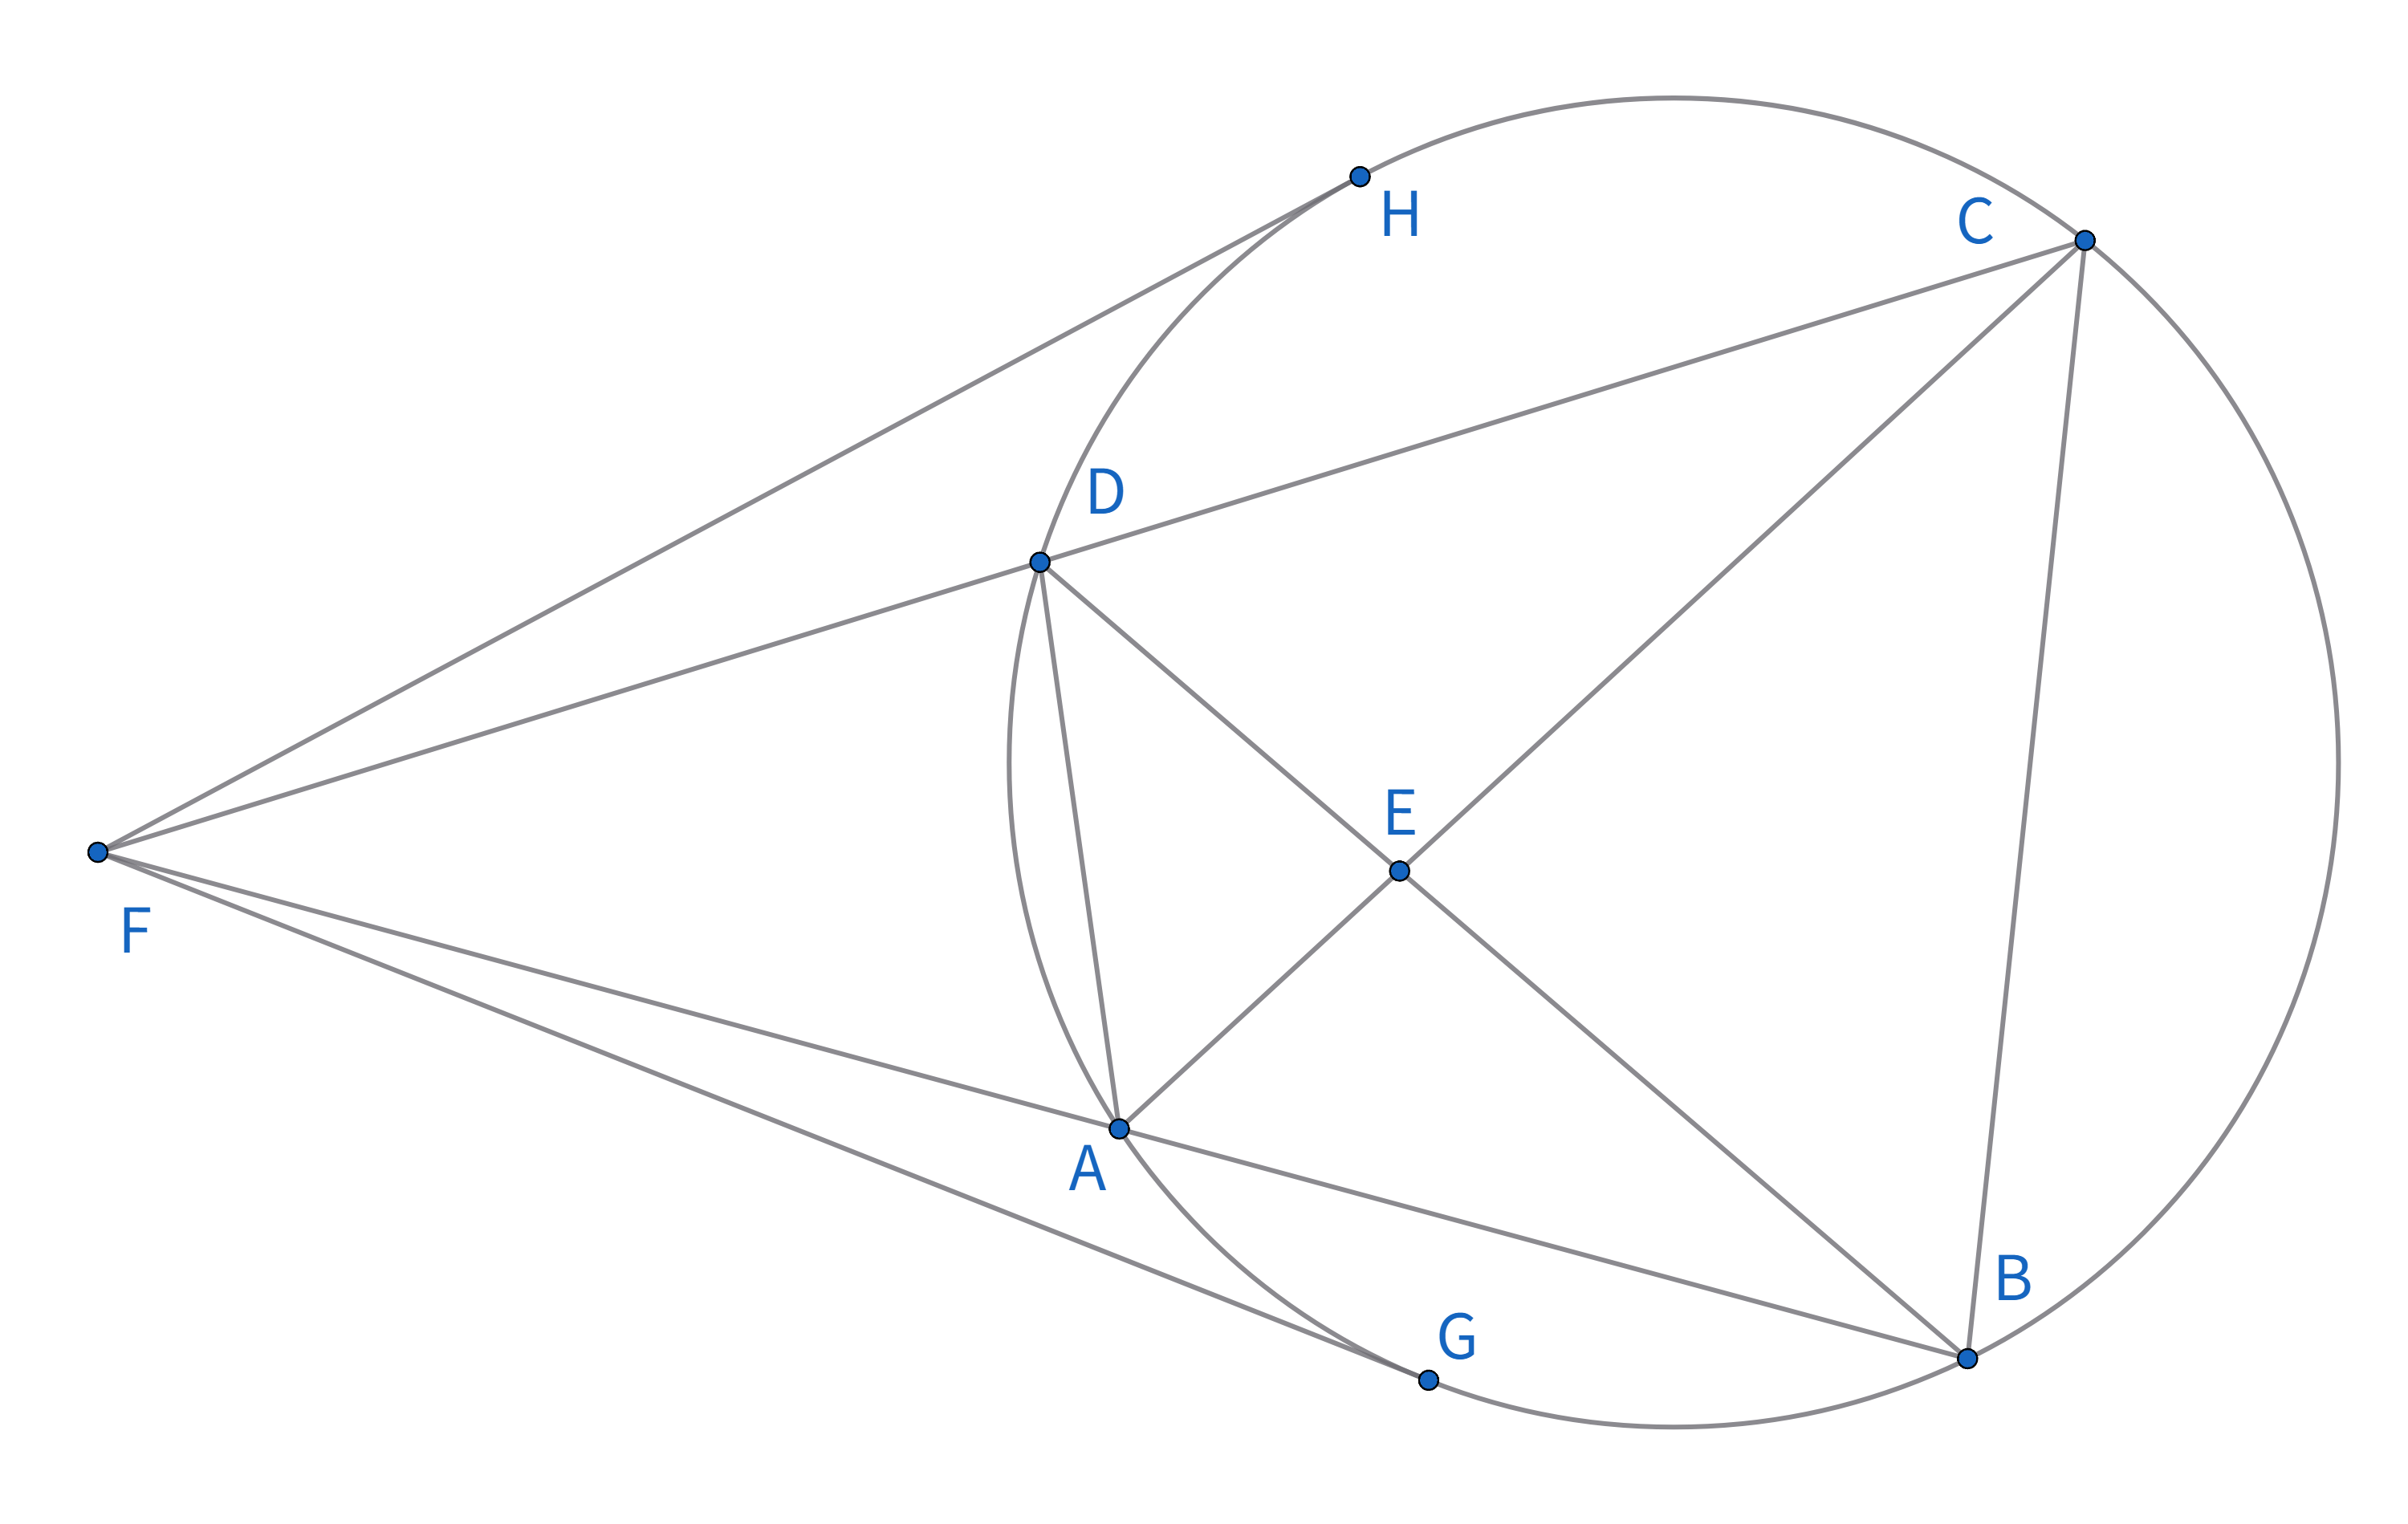
\includegraphics[width=0.7\linewidth]{figures/圆幂定理.png}
    \caption{圆幂定理}
\end{figure}
\begin{remark}
    定点到定圆的圆幂是一个定值,与割线的取法无关。
\end{remark}


\begin{theorem}[圆幂逆定理]
    设 $A, B, C, D$ 是平面上四个不同的点,直线 $AB$ 和 $CD$ 相交于 $P$。假设 $P$ 或者同时在两条线段 $AB$ 和 $CD$ 内,或者同时在两条线段外。若 $PA \cdot PB = PC \cdot PD$,则 $A, B, C, D$ 四点共圆。
\end{theorem}

%-------------------------------------------------------------
\newpage 
\section{根轴}
\begin{theorem}[根轴]
    对于两已知圆有等幂点的轨迹,为一条垂直于连心线的直线。
\end{theorem}
\begin{figure}[H]
    \centering
    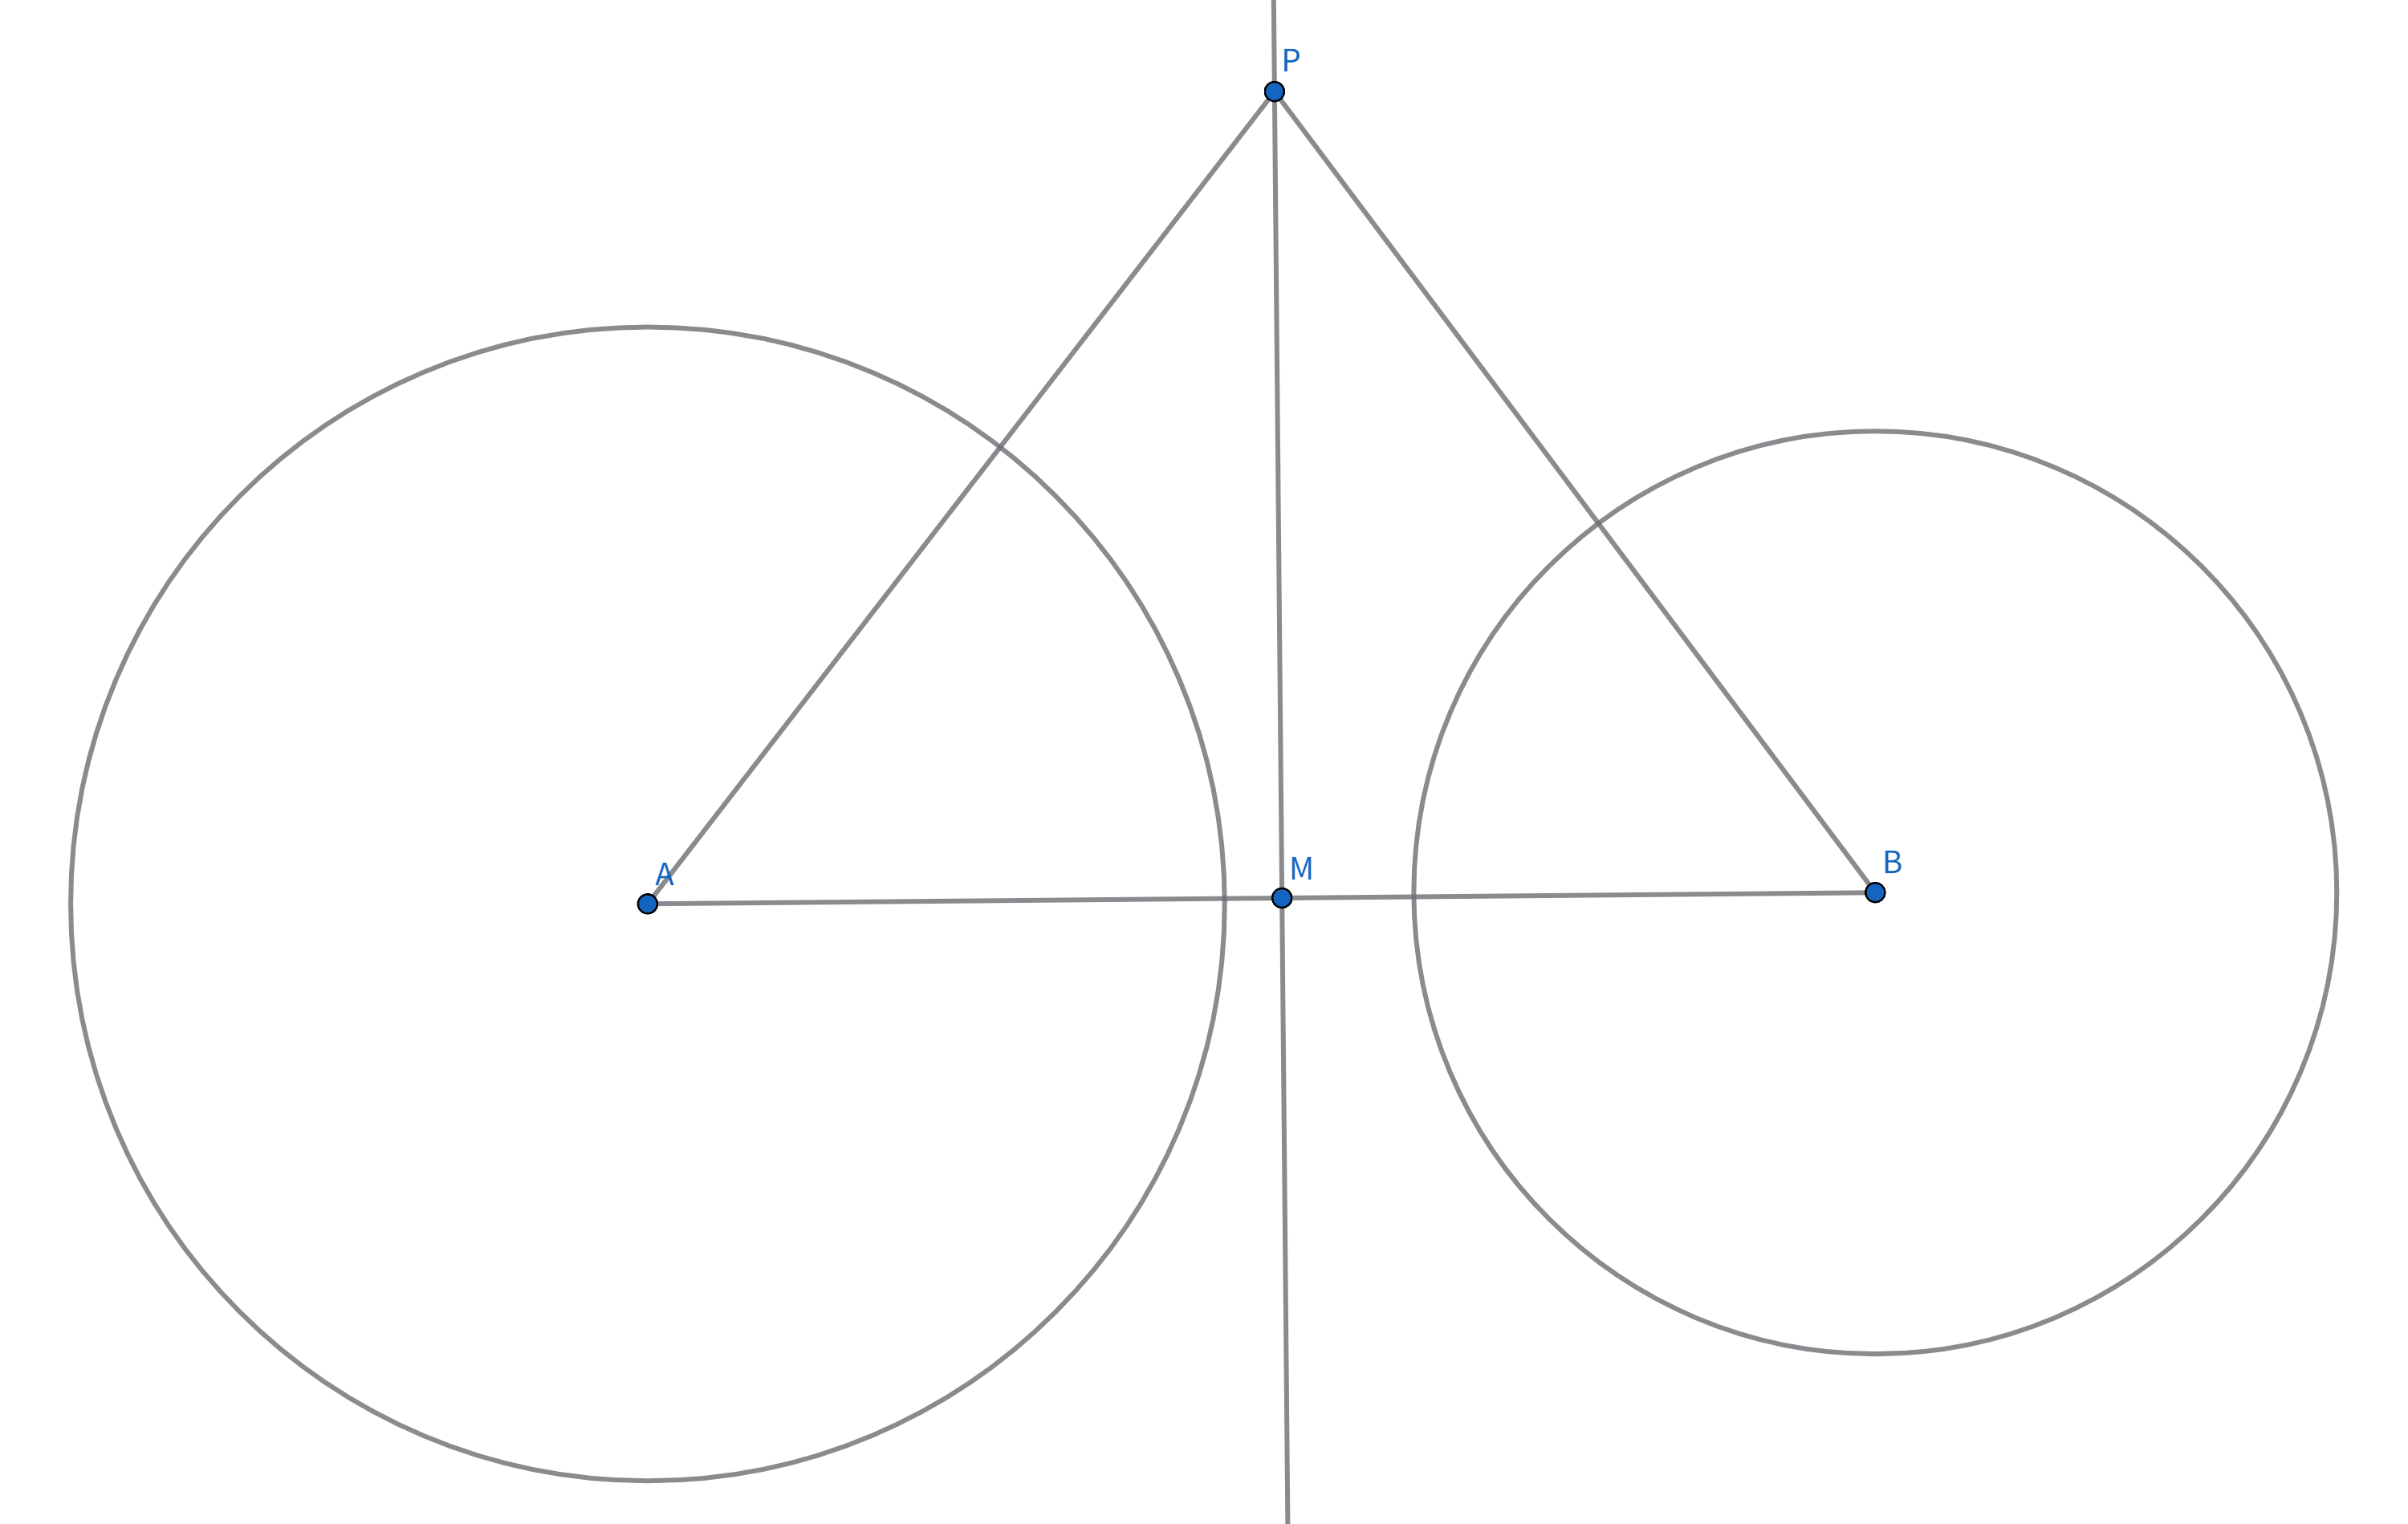
\includegraphics[width=0.7\linewidth]{figures/根轴.png}
    \caption{根轴}
\end{figure}

\begin{proposition}[根轴性质]
    两圆的根轴有如下性质:
    
    (1) 若两圆相交,其根轴就是公共弦所在的直线。
    
    (2) 若两圆相切(内切或外切),其根轴就是过两圆切点的公切线。
    
    (3) 若两圆外离,则两圆的四条公切线的中点在根轴上。
\end{proposition}
\begin{figure}[H]
    \centering
    \hfill % 添加一些水平间距
    \begin{minipage}[t]{0.3\textwidth}
        \centering
        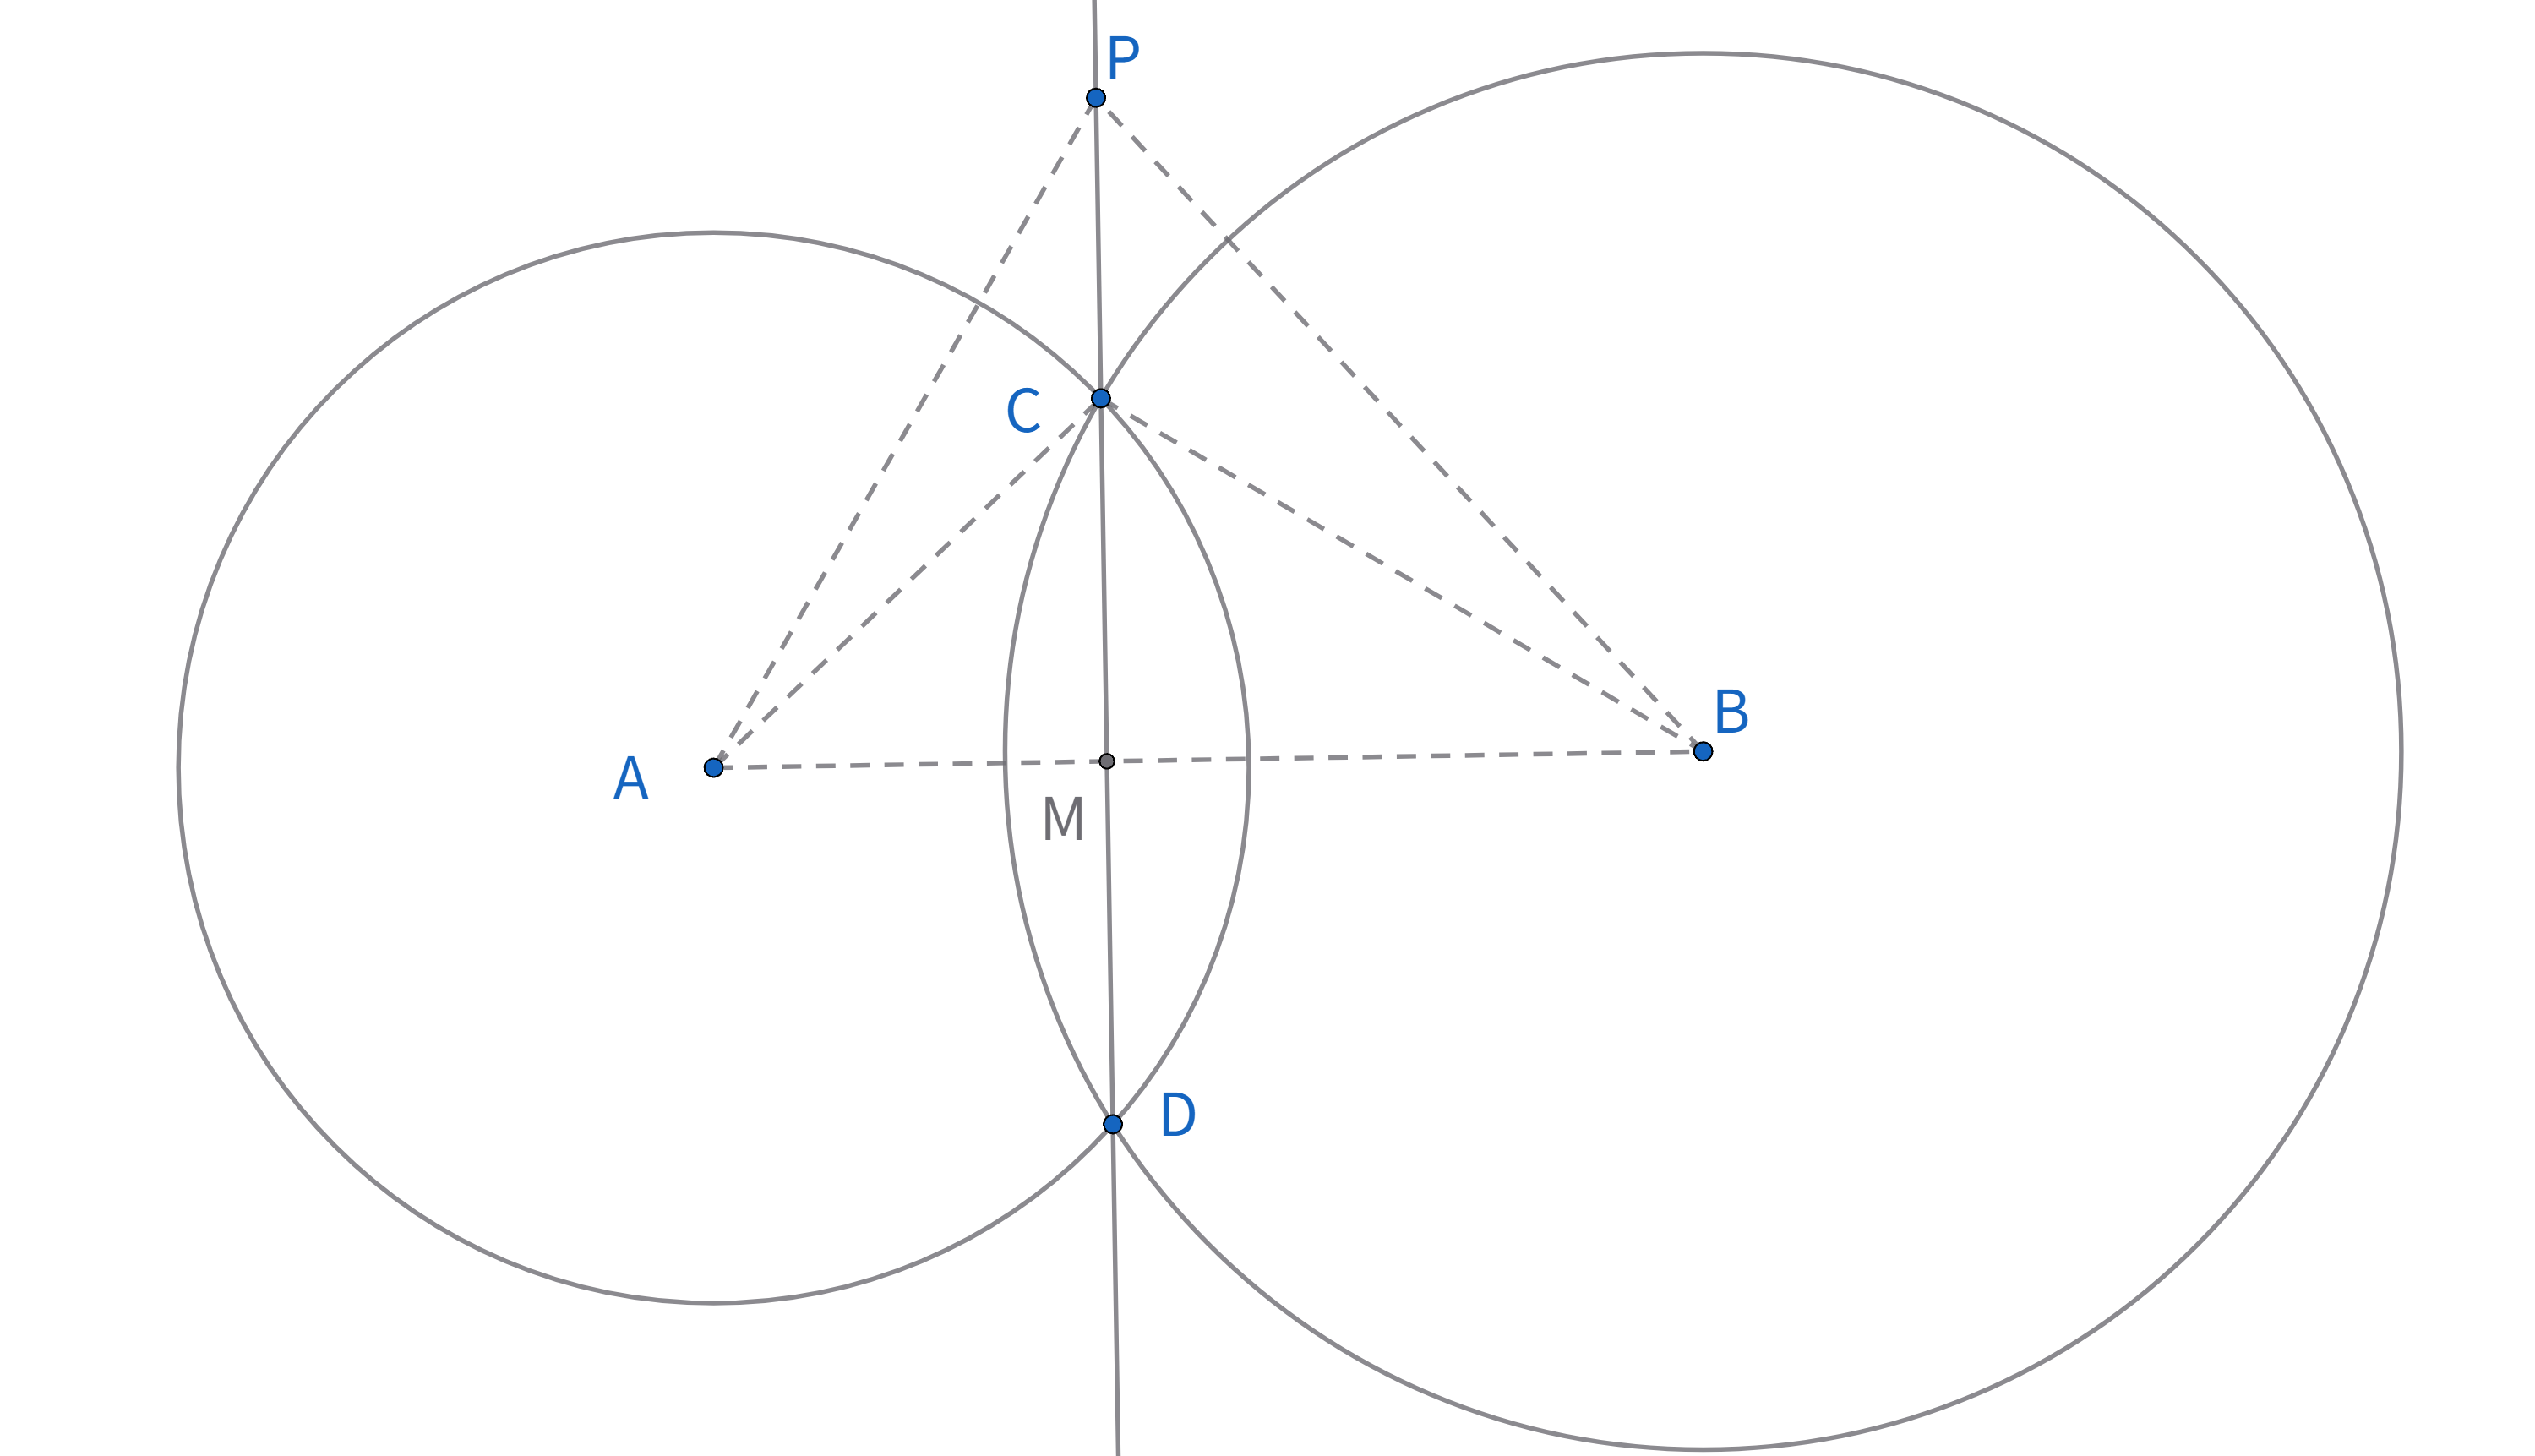
\includegraphics[width=\linewidth]{figures/相交圆根轴.png}
        \caption{相交圆根轴}
    \end{minipage}
    \hfill % 添加一些水平间距
    \begin{minipage}[t]{0.3\textwidth}
    \centering
    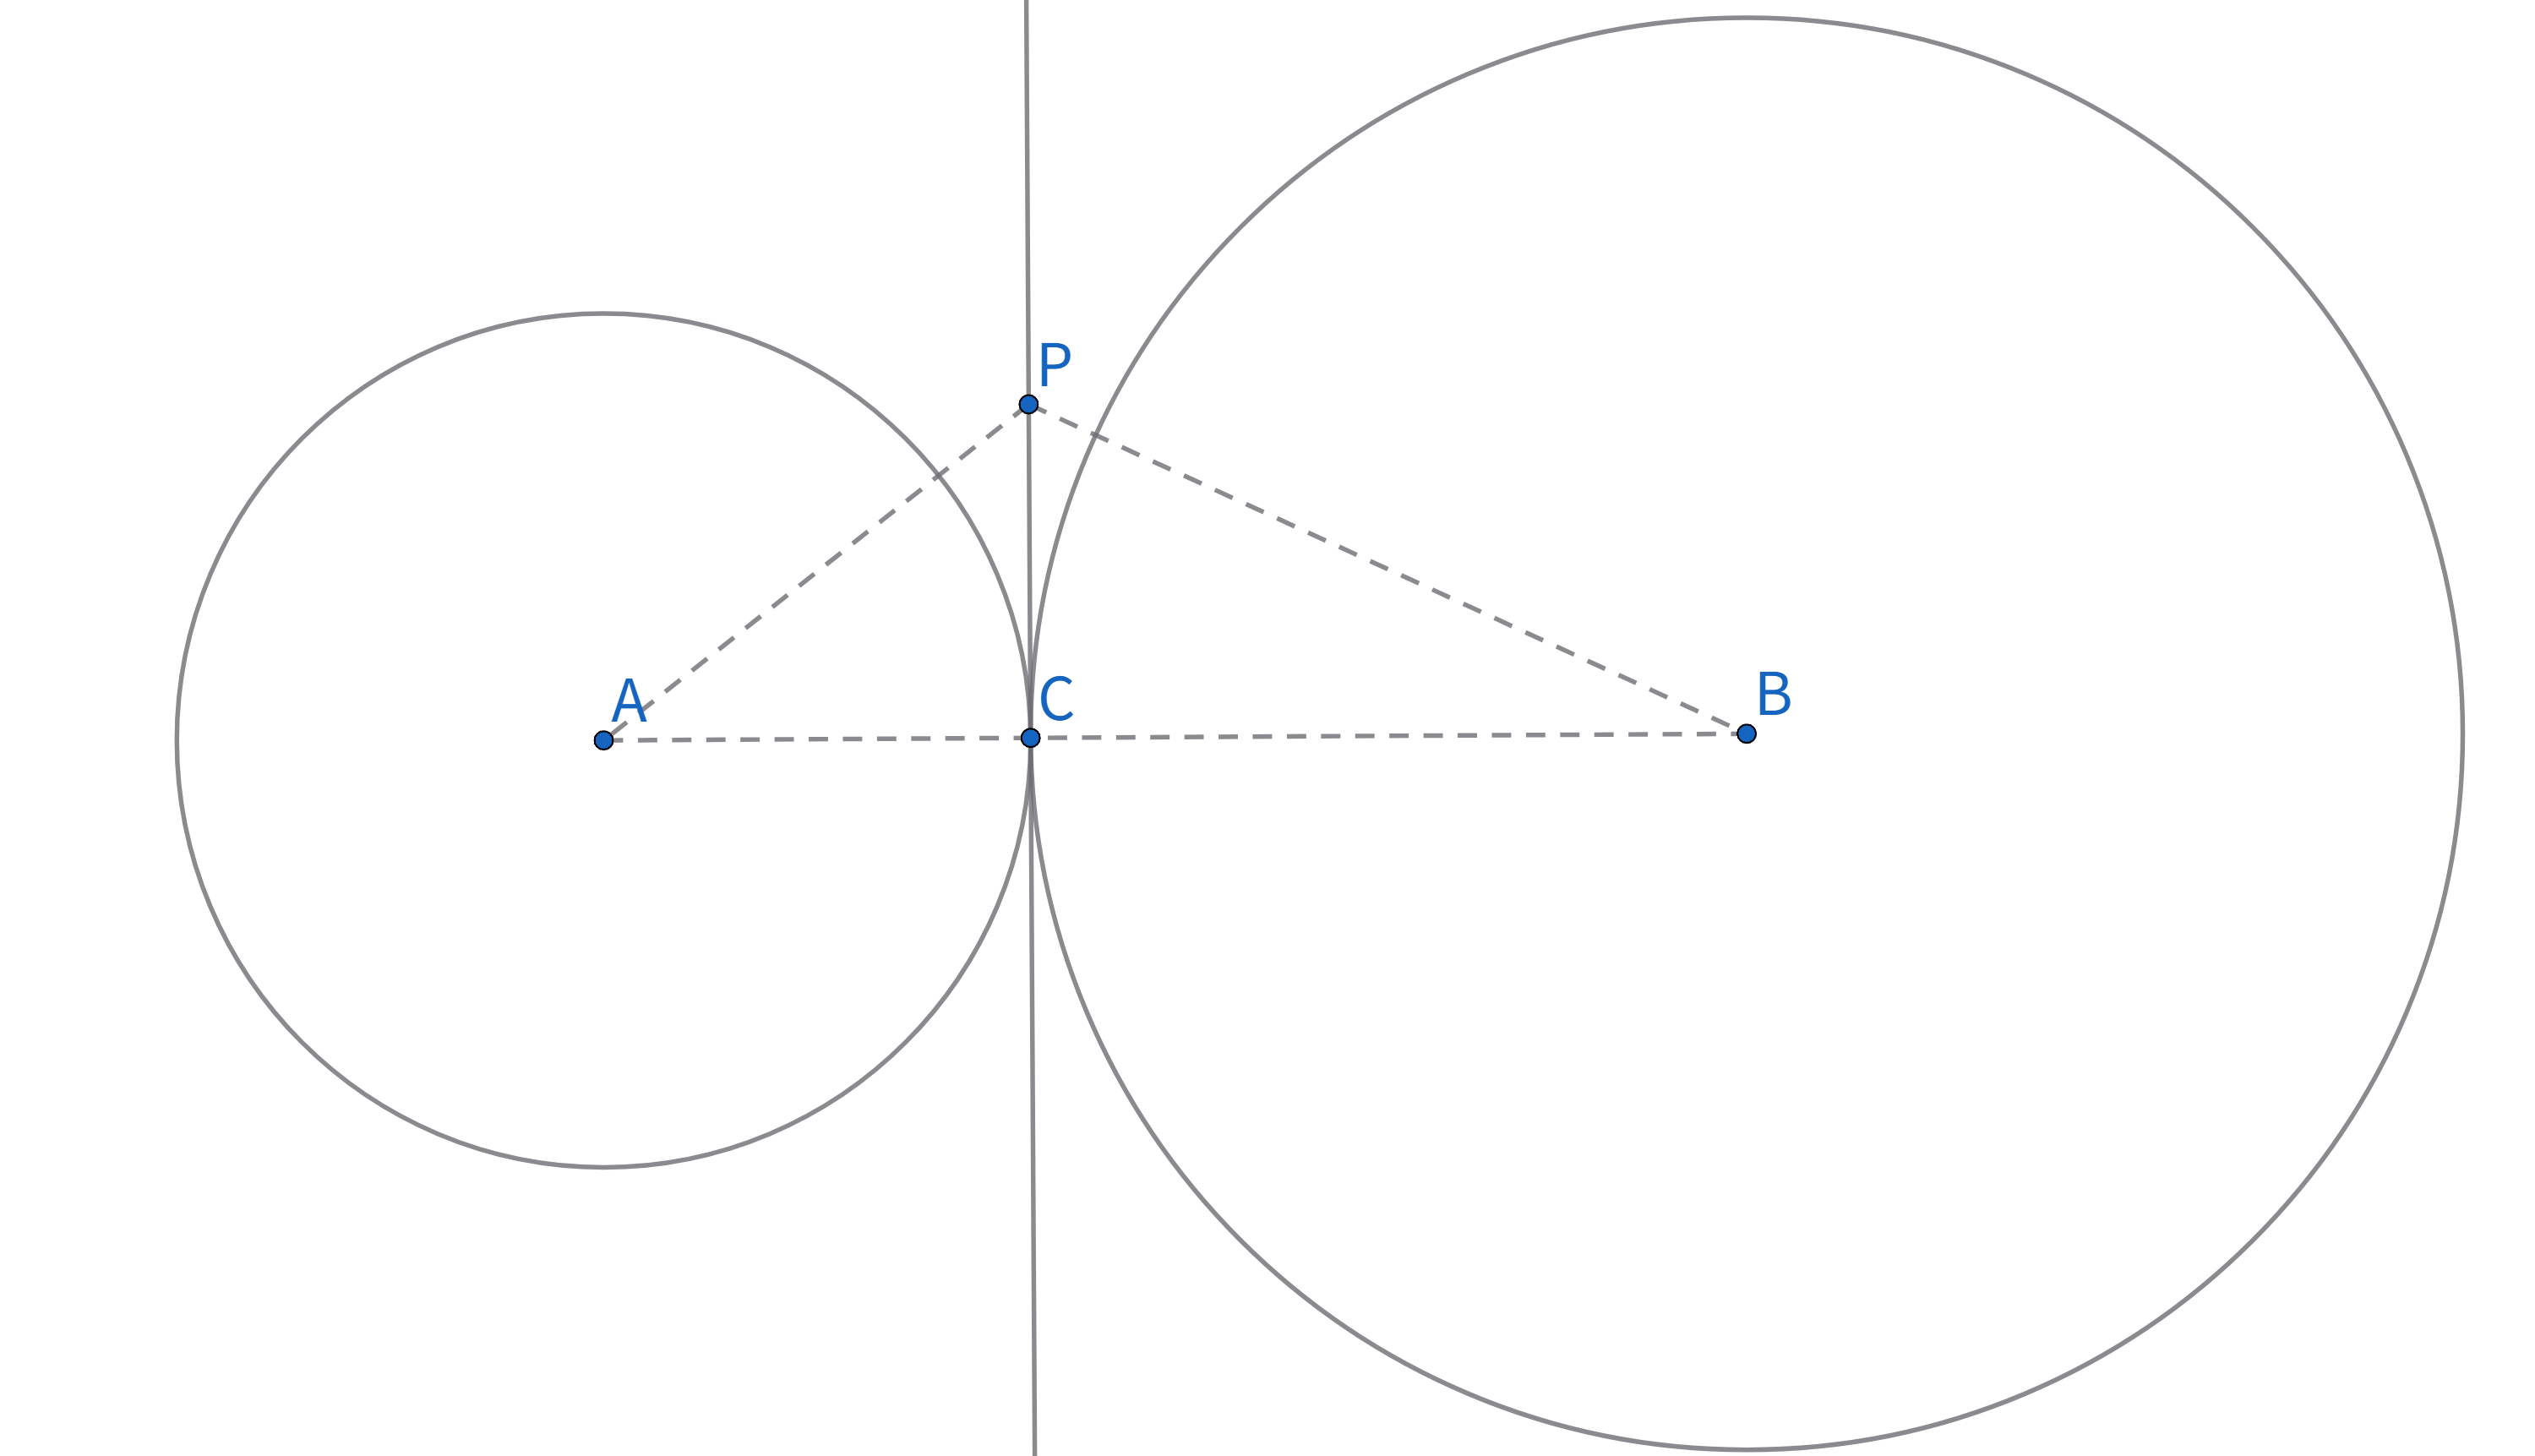
\includegraphics[width=\linewidth]{figures/相切圆根轴.png}
    \caption{相切圆根轴}
    \end{minipage}
    \begin{minipage}[t]{0.3\textwidth}
    \centering
    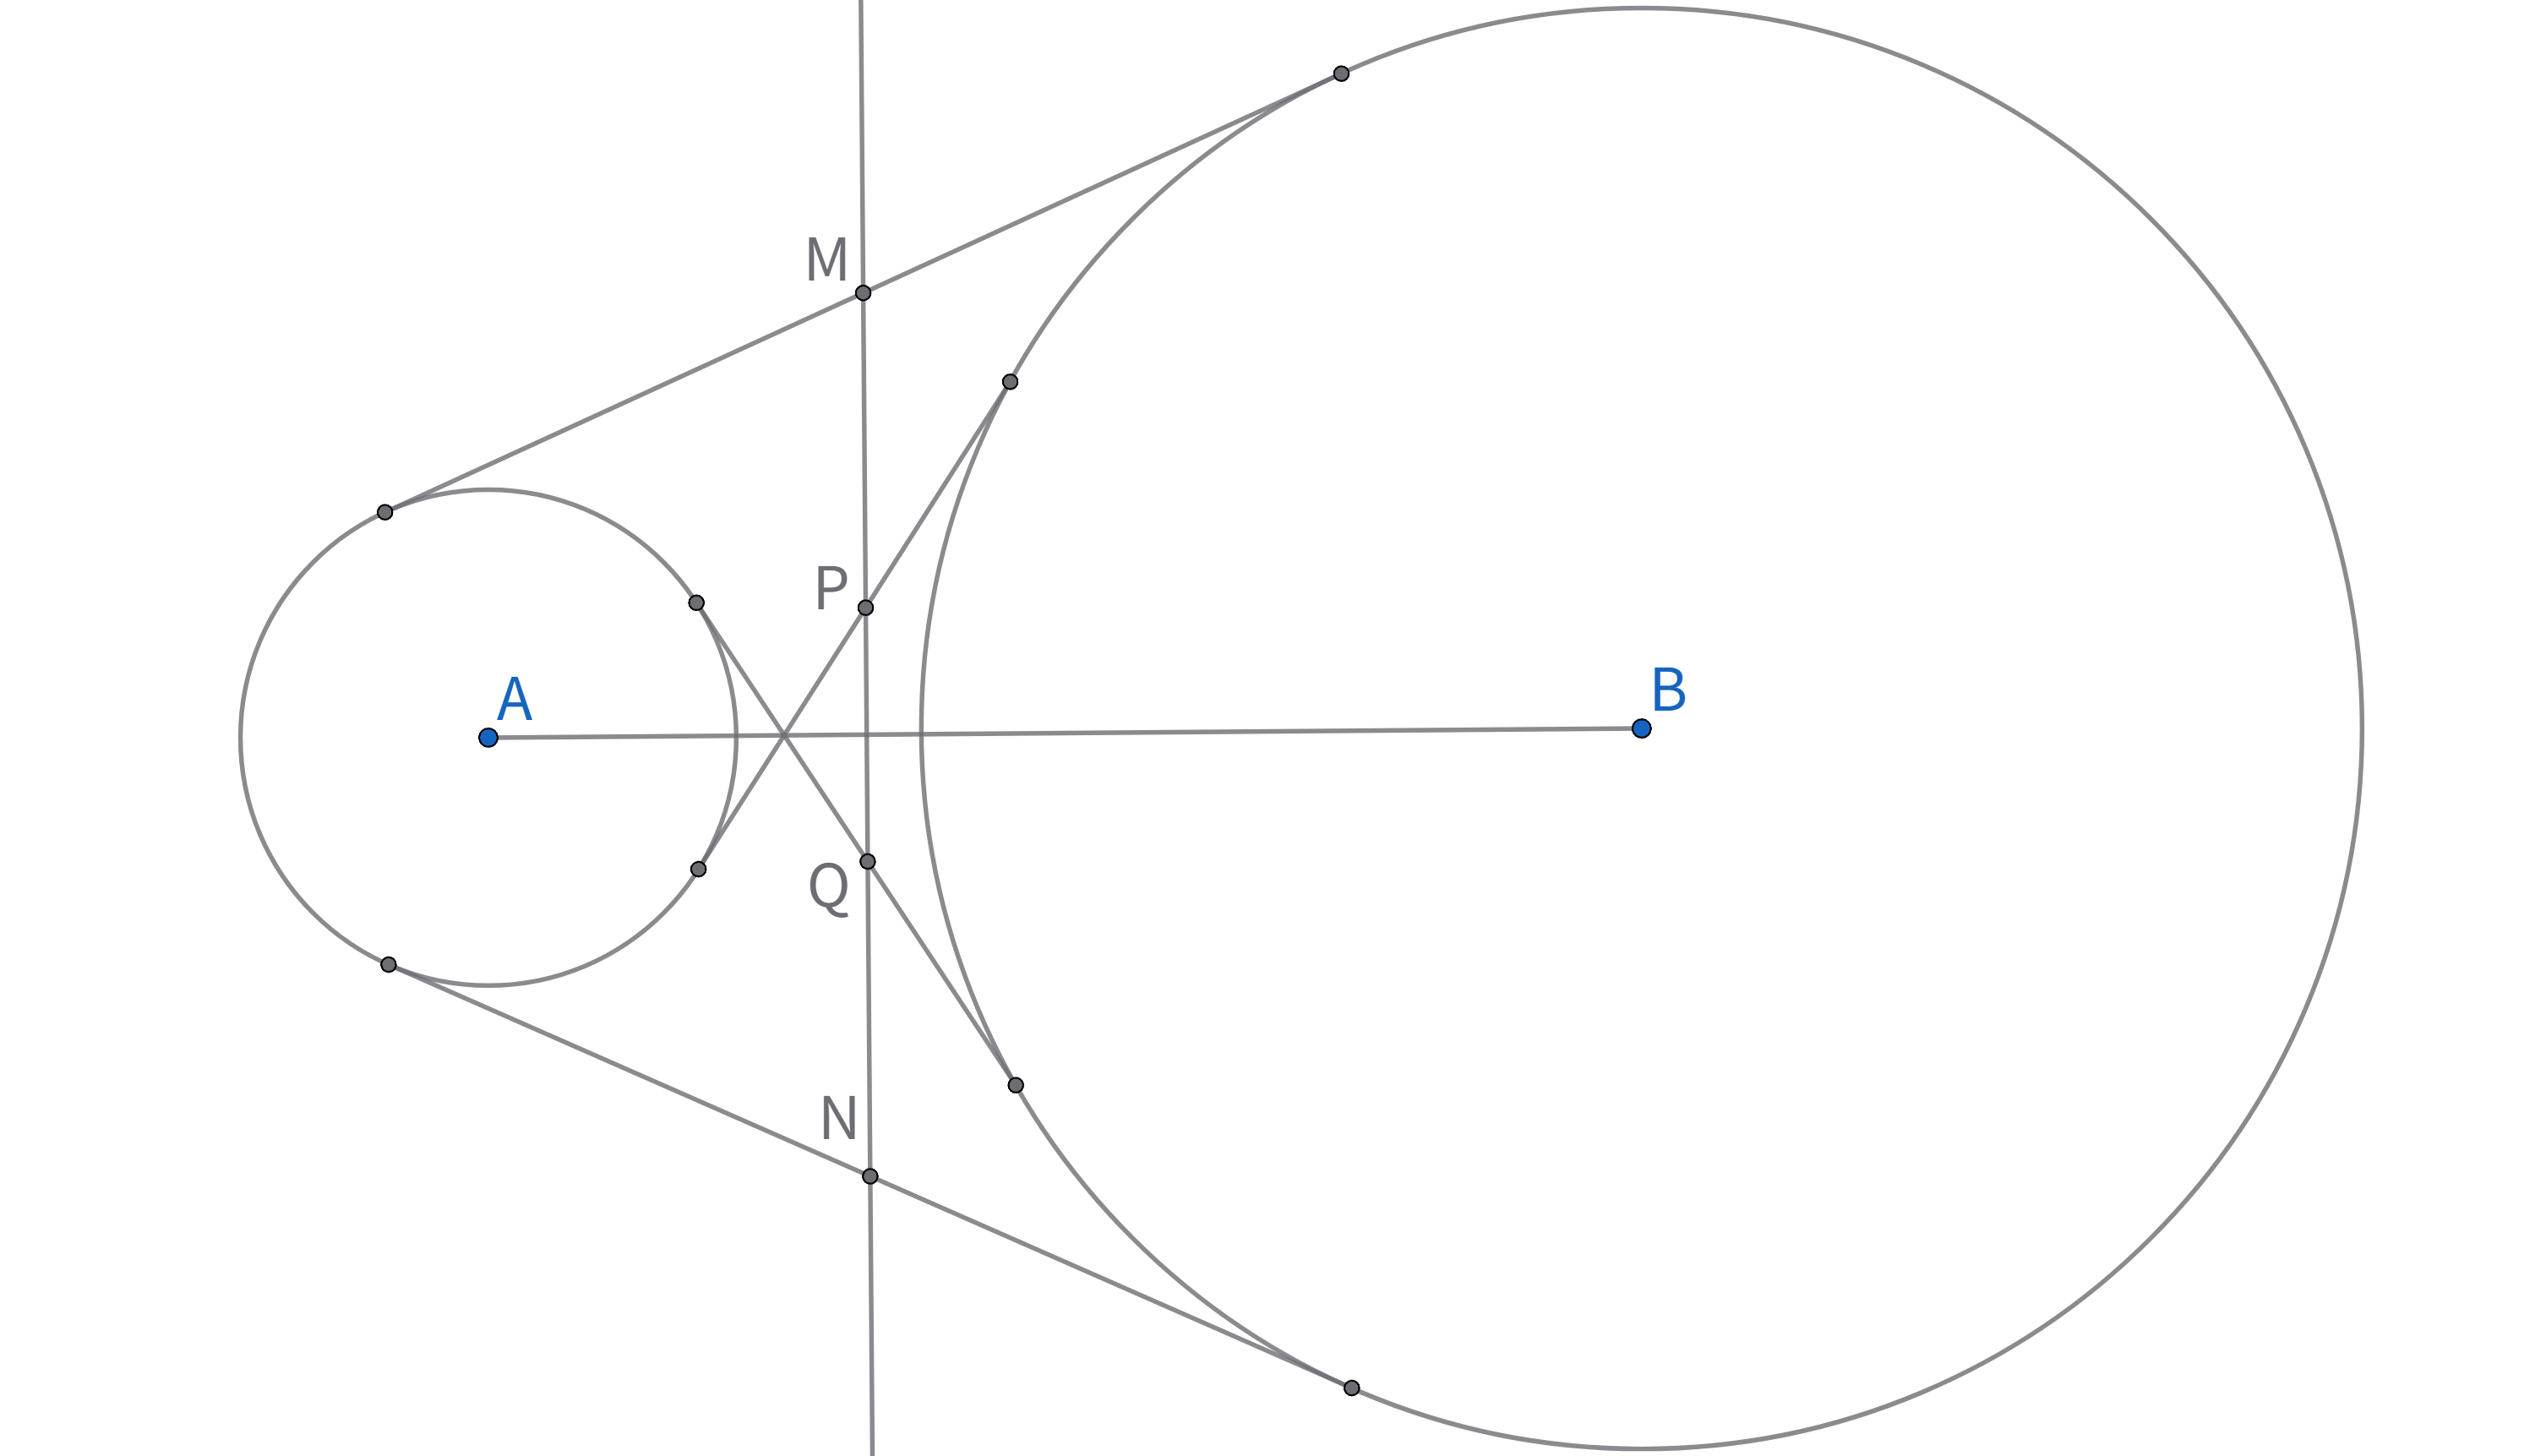
\includegraphics[width=\linewidth]{figures/相离圆根轴.png}
    \caption{相离圆根轴}
    \end{minipage}
\end{figure}


\begin{exercise}
    设 $P$ 在 $\triangle ABC$ 的内部,假设 $BC$ 与 $\triangle ABP$ 和 $\triangle ACP$ 的外接圆均相切。证明:射线 $AP$ 平分 $\overline{BC}$。
\end{exercise}

\begin{exercise}
    用根轴证明三角形的垂心存在,也就是说,若 $AD, BE, CF$ 是 $\triangle ABC$ 的三个高,证明它们共点。
\end{exercise}



%-------------------------------------------------------------
\newpage 
\section{根心}
\begin{theorem}[根心定理]
    平面内的三个定圆,他们两两的根轴或相交于一点,或互相平行。
\end{theorem}
\begin{figure}[H]
    \centering
    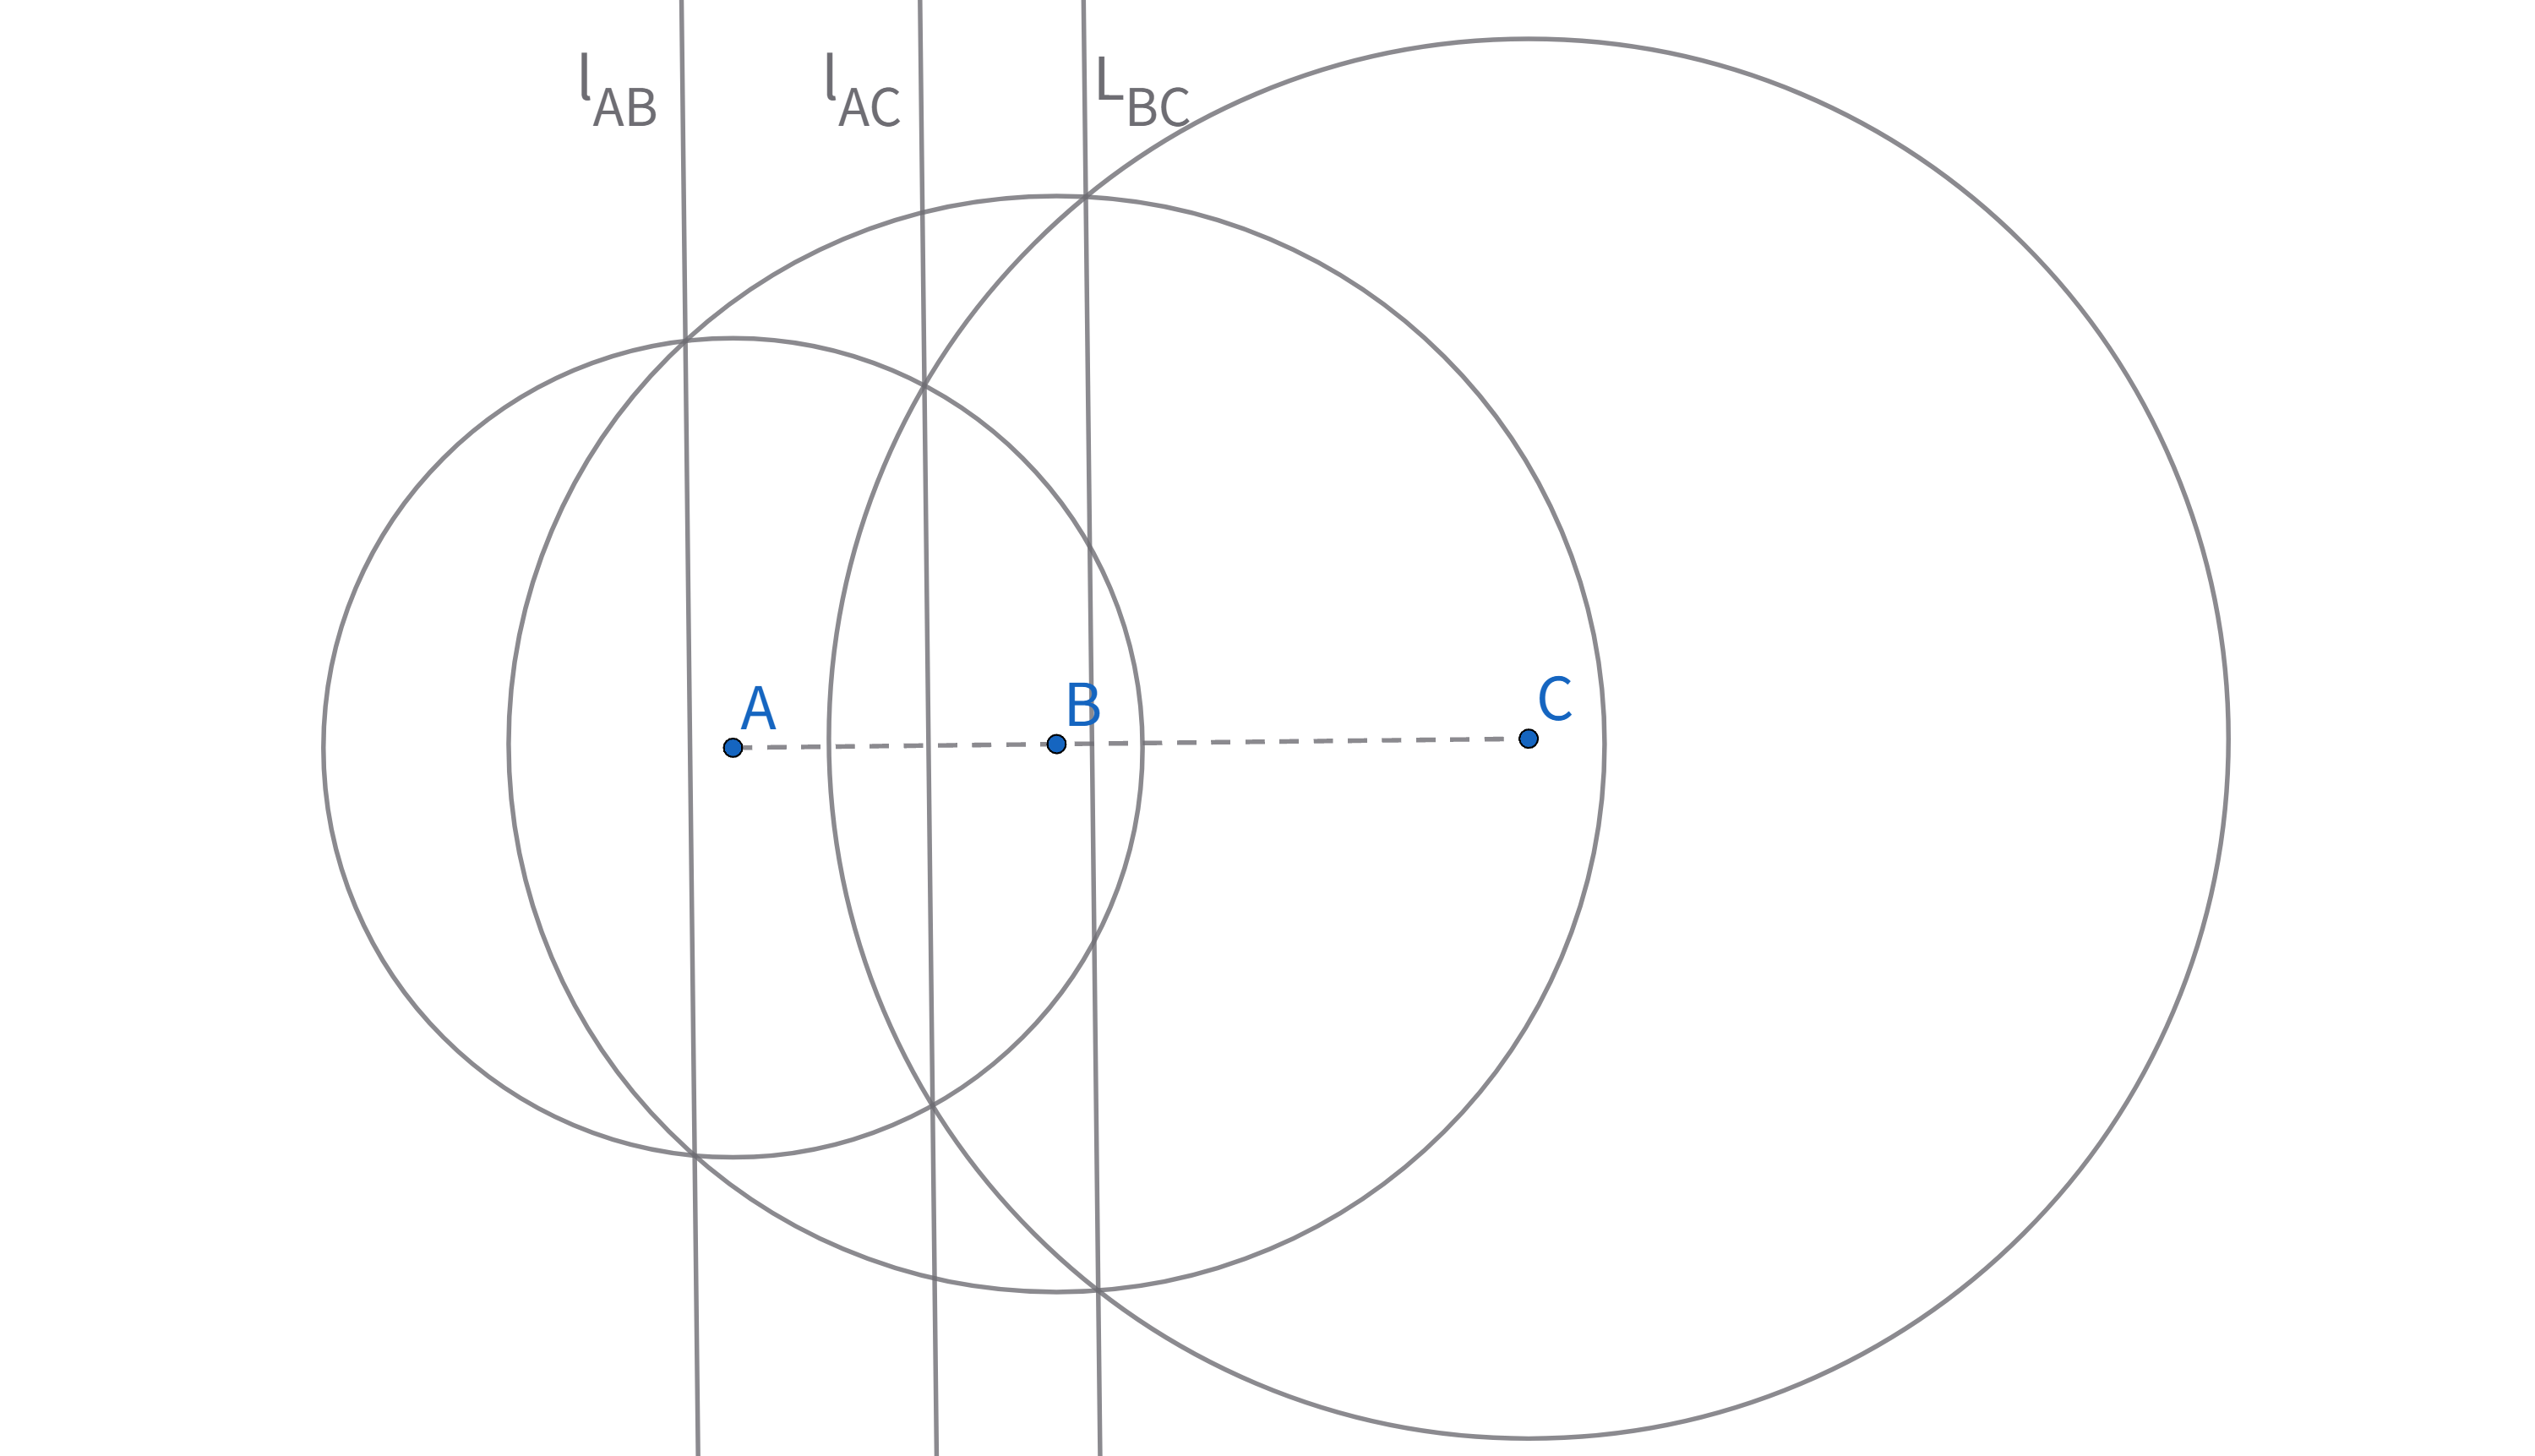
\includegraphics[width=0.8\linewidth]{figures/平行根轴.png}
    \caption{平行根轴}
\end{figure}
\begin{figure}[H]
    \centering
    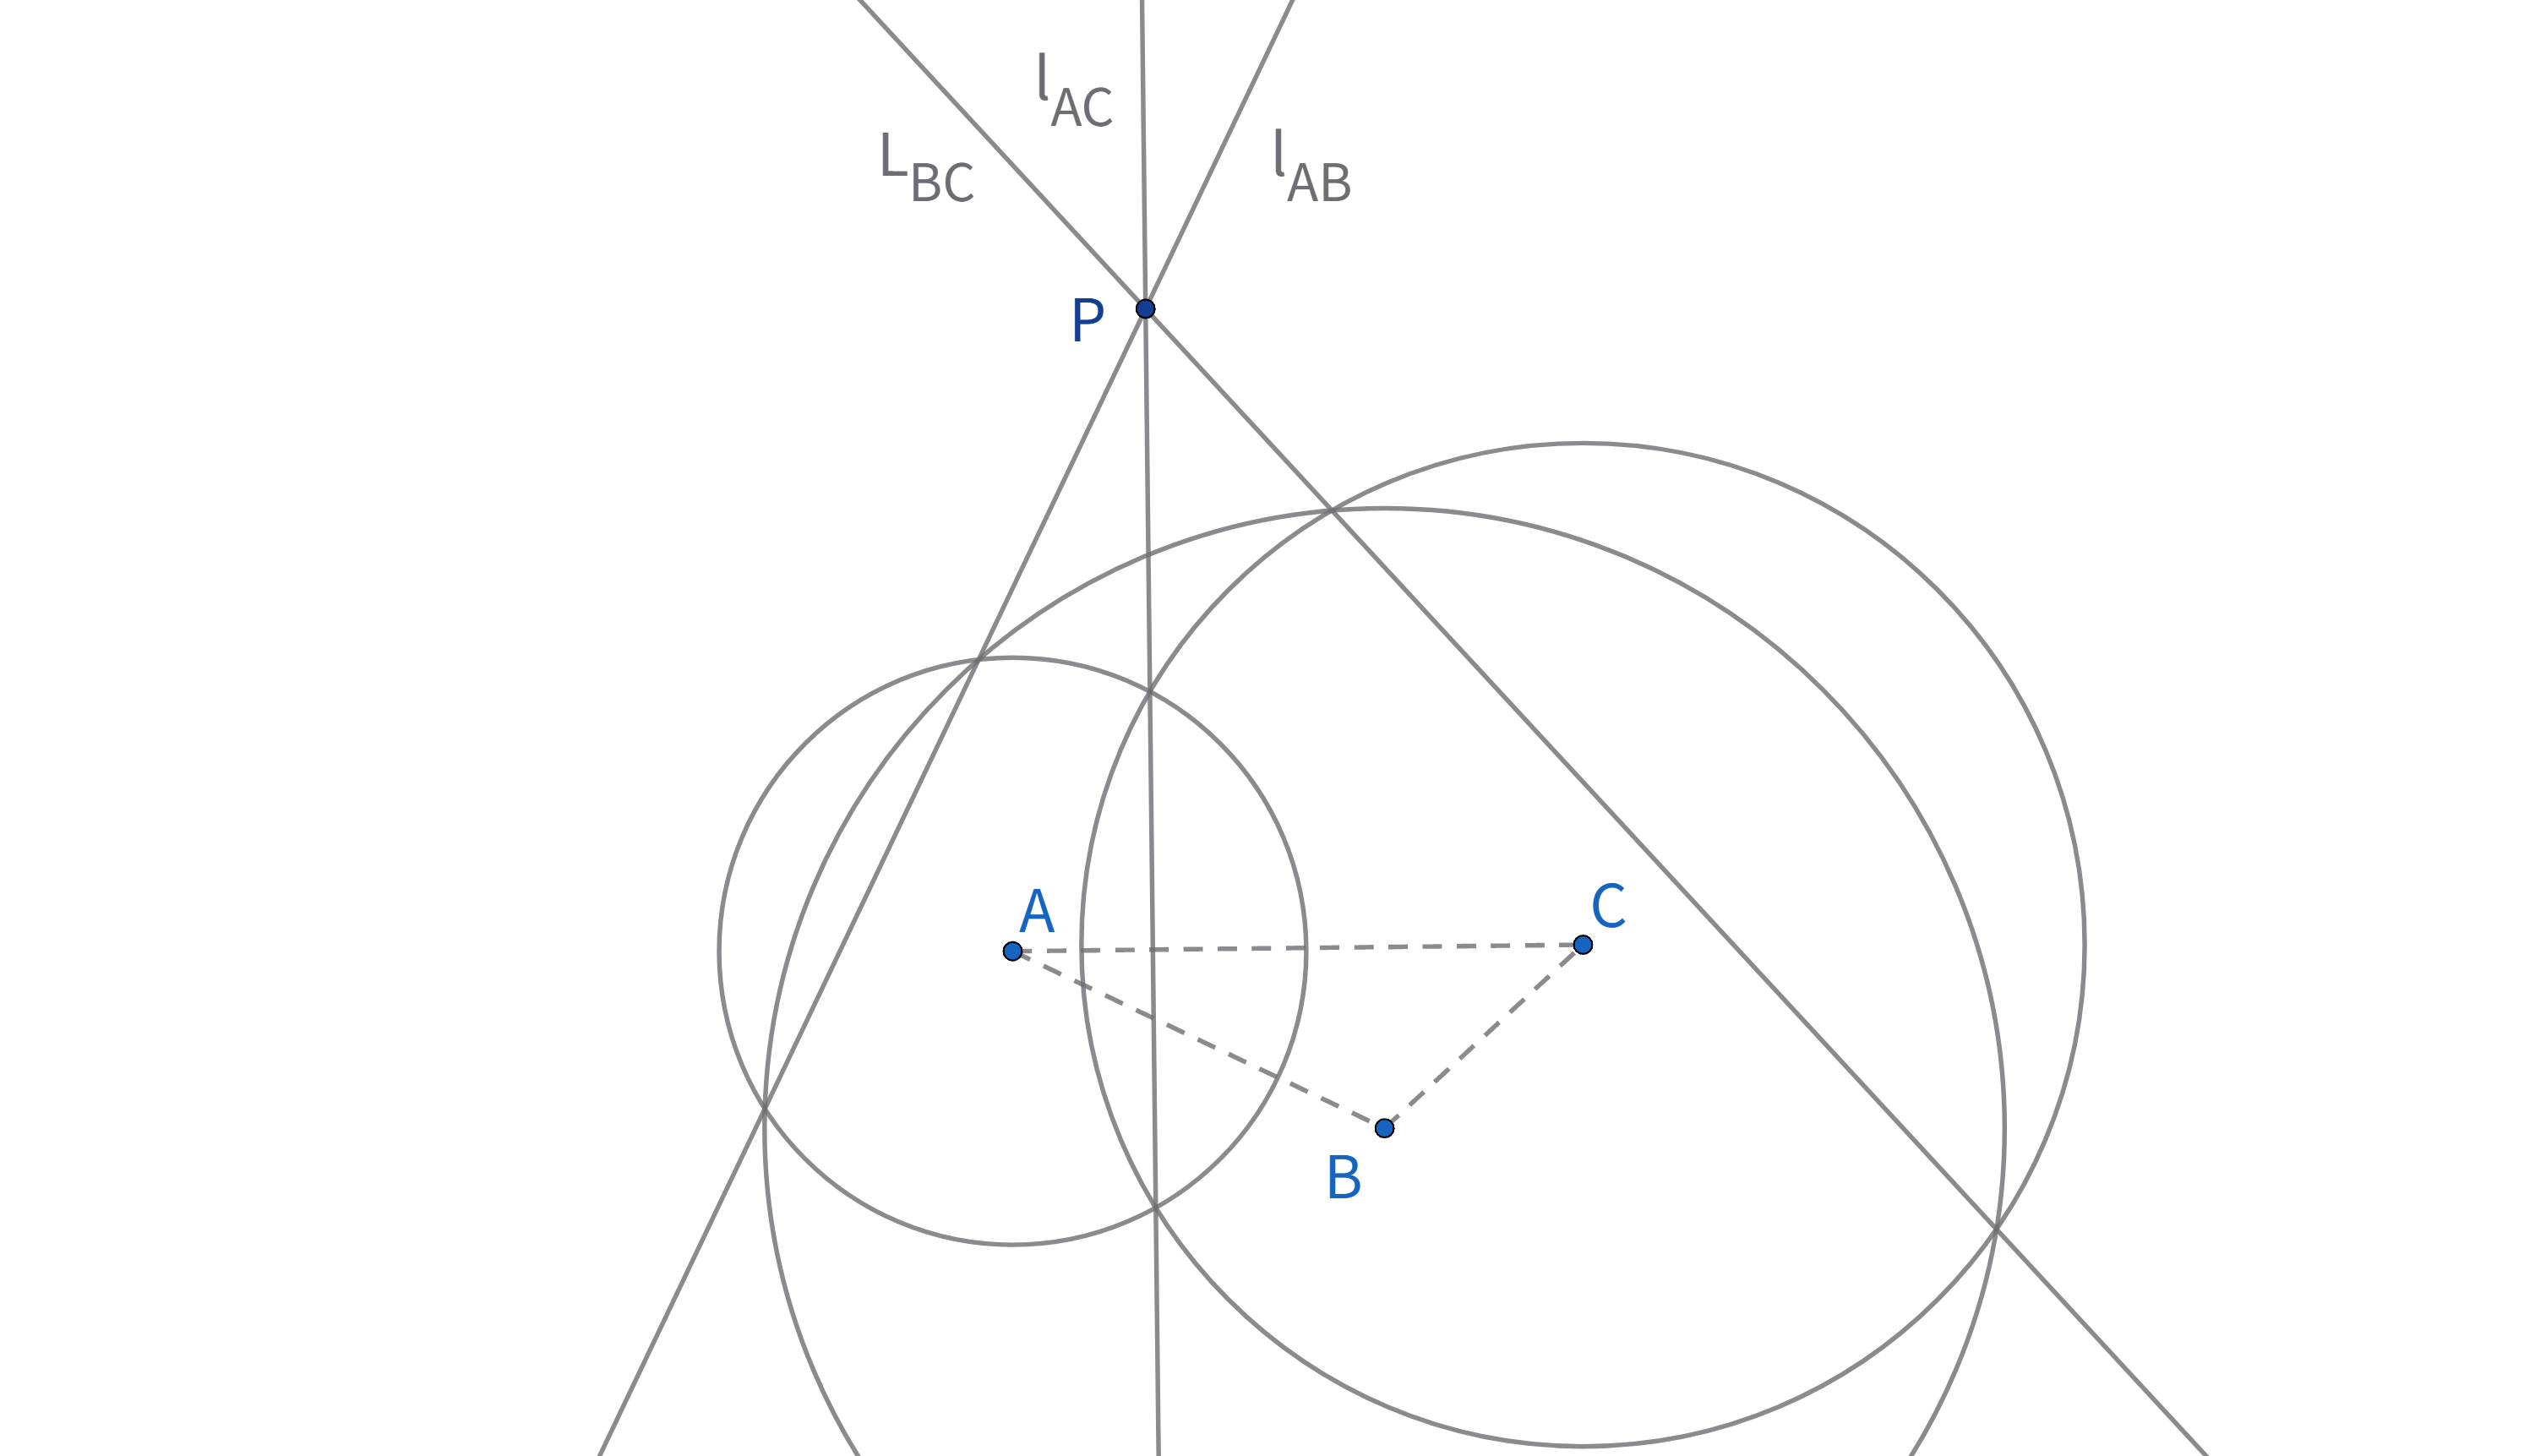
\includegraphics[width=0.8\linewidth]{figures/根心.png}
    \caption{根心}
\end{figure}

% \part{四点共圆}
\section{判定方法}
\begin{proposition}[四点共圆判定方法]
    四边形ABCD顶点均在圆O上,等价于下列任一条件成立。

    (1) A、B、C、D到同一点O的距离相同。

    (2) 存在一组对角互补。

    (3) 有一边与另两点构成的顶角度数相同。

    (4) 对角线交于F点,$AF\cdot FC = BF\cdot FD$。

    (5) 有一组对边AB、CD的延长线相交于E,若$EA\cdot EB = ED\cdot EC$。
\end{proposition}
\begin{figure}[H]
    \centering
    \includegraphics[width=\linewidth]{figures/四点共圆.png}
    % \caption{Caption}
    % \label{fig:enter-label}
\end{figure}




% 蝴蝶定理
\section{蝴蝶定理}
\begin{theorem}
    设M为圆内弦PQ的中点,过M作弦AB和CD。设AD和BC各相交PQ弦于点X和Y,则M是XY的中点。
\end{theorem}

\begin{figure}[H]
    \centering
    \hfill % 添加一些水平间距
    \begin{minipage}[t]{0.45\textwidth}
    \centering
    \includegraphics[width=\linewidth]{figures/蝴蝶定理.png}
    \end{minipage}
    \hfill % 添加一些水平间距
    \begin{minipage}[t]{0.45\textwidth}
    \centering
    \includegraphics[width=\linewidth]{figures/蝴蝶定理辅助线.png}
    \end{minipage}
\end{figure}



\section{托勒密(Ptolemy)定理}
\begin{theorem}
    圆的内接四边形对角线乘积等于两组对边乘积之和。
    $$AC \cdot BD = AB \cdot CD + BC \cdot AD.$$
\end{theorem}
\begin{figure}[H]
    \centering
    \includegraphics[width=0.7\linewidth]{figures/托勒密定理.png}
    \caption{托勒密定理}
\end{figure}


% \include{Exercises/圆与圆.tex}
% 


% \section{计算法}
\subsection{面积法}
\begin{proposition}
    对任意 $\triangle ABC$,设$BC=a,AC=b,AB=c$。其面积可以表示为
    $$S_{\triangle ABC} =\frac{1}{2}bc\sin A=\frac{1}{2}ac\sin B=\frac{1}{2}ab\sin C$$
\end{proposition}
\begin{proof}
    过点A作BC的垂线交BC于D点,由三角形面积公式可知
    $$S_{\triangle ABC} = \frac{1}{2} BC \cdot AD = \frac{1}{2} a \cdot (\sin B \cdot AB) = \frac{1}{2} ac \sin B.$$
    其他同理可以证明。
\end{proof}


\subsection{三角法}
\begin{proposition}
    给定$0<\alpha_1,\alpha_2,\beta_1,\beta_2<180^\circ$,满足$\alpha_1+\beta_1=\alpha_2+\beta_2 < 180^\circ$,若
    $$
    \frac{\sin\alpha_1}{\sin\beta_1}= \frac{\sin\alpha_2}{\sin\beta_2},
    $$
    则一定有$\alpha_1=\alpha_2,\quad \beta_1 =\beta_2$。
\end{proposition}


\newpage 
\subsection{分角线定理}
\begin{theorem}[分角线定理]
    在$\triangle ABC$中,D是BC所在直线上异于B、C的一点,连结AD,则有
    $$
    \frac{BD}{DC} = \frac{AB\sin \angle BAD}{AC \sin \angle CAD}.
    $$
\end{theorem}
\begin{figure}[ht]
    \centering
    \includegraphics[width=0.7\linewidth]{figures/分角线定理.png}
    \caption{分角线定理}
\end{figure}
\begin{proposition}[角平分线定理]
在$\triangle ABC$中,$\angle A$的角平分线交BC边于D,则有
    $$
    \frac{BD}{DC} = \frac{AB}{AC}.
    $$
\end{proposition}

\begin{proposition}[中线定理]
    在$\triangle ABC$中,$\angle A$的角平分线交BC边于D,则有
    $$
    \frac{AC}{AB} = \frac{\sin \angle BAD}{\sin \angle CAD}.
    $$
\end{proposition}

\begin{figure}[htbp]
    \centering
    \hfill % 添加一些水平间距
    \begin{minipage}[t]{0.45\textwidth}
    \centering
    \includegraphics[width=\linewidth]{figures/分角线定理 -角平分线.png}
    \end{minipage}
    \hfill % 添加一些水平间距
    \begin{minipage}[t]{0.45\textwidth}
    \centering
    \includegraphics[width=\linewidth]{figures/分角线定理-中线.png}
    \end{minipage}
\end{figure}

\newpage 
\subsection{共边三角形}
\begin{proposition}
    $\triangle ABC,\triangle ABD$共用BC边,有下列等式成立:
    $$
    \frac{\sin\angle BAC}{\sin\angle BAD} = \frac{BC}{BD}\cdot \frac{\sin\angle ACB}{\sin\angle ADB}.
    $$
\end{proposition}
\begin{figure}[ht]
    \centering
    \includegraphics[width=0.7\linewidth]{figures/共边三角形.png}
    \caption{共边三角形}
\end{figure}



\newpage 
\subsection{托勒密(Ptolemy)定理}
\begin{theorem}[托勒密定理]
    圆的内接四边形对角线乘积等于两组对边乘积之和。
    $$AC \cdot BD = AB \cdot CD + BC \cdot AD.$$
\end{theorem}
\begin{figure}[ht]
    \centering
    \includegraphics[width=0.7\linewidth]{figures/托勒密定理.png}
    \caption{托勒密定理}
\end{figure}

\subsubsection{三弦定理}
\begin{theorem}[三弦定理]
    如果A是圆上任意一点,AB、ACAD是该圆上顺次的三条弦,则
    $$
    AC\cdot \sin \angle BAD = AB\cdot \sin \angle CAD+AD\cdot \sin \angle CAB
    $$
\end{theorem}

\newpage 
\subsubsection{直线上的托勒密定理}
\begin{theorem}[直线上的托勒密定理]
    若A、B、C、D为一条直线上依次排列的四点,则
    $$AC \cdot BD = AB \cdot CD + BC \cdot AD.$$
\end{theorem}
\subsubsection{托勒密不等式}
\begin{theorem}[托勒密不等式]
    ABCD为任意凸四边形,则
    $$AB \cdot CD + BC \cdot AD\leq AC \cdot BD.$$
    当且仅当ABCD四点共圆时取得等号。
\end{theorem}
\begin{figure}[htbp]
    \centering
    \includegraphics[width=0.7\linewidth]{figures/托勒密不等式.png}
    \caption{托勒密不等式}
\end{figure}

\newpage 
\subsection{斯特瓦尔特(Stewart)定理}
\begin{theorem}[斯特瓦尔特定理]
    B、P、C依次分别为A点引出的三条射线上的点,则等式
    $$
    AB^2\cdot PC+AC^2\cdot PB = AP^2\cdot BC + PB\cdot PC\cdot BC.
    $$
    等价于B、P、C三点共线。
\end{theorem}
\begin{figure}[ht]
    \centering
    \includegraphics[width=0.7\linewidth]{figures/斯特瓦尔特定理.png}
    \caption{斯特瓦尔特定理}
\end{figure}


\newpage
\subsection{定差幂线}
\begin{theorem}[定差幂线定理]
    设MN、PQ是两条线段,则$MN\perp PQ$的充分必要条件是
    $$PM^2-PN^2 = QM^2-QN^2$$.
\end{theorem}
\begin{figure}[ht]
    \centering
    \includegraphics[width=0.7\linewidth]{figures/定差幂线.png}
    \caption{定差幂线}
\end{figure}


\newpage 
\subsection{张角定理}
\begin{theorem}[张角(Spread Angle)定理]
    A、C、B依次分别是平面内一点P所引三条射线上的点,AC、CB对P的张角分别为$\alpha,\beta$,并且$\alpha+\beta<180^circ$,则A、C、B共线的充分必要条件是
    $$
    \frac{\sin(\alpha+\beta)}{PC}
    = \frac{\sin\alpha}{PB}
    +\frac{\sin\beta}{PA}.
    $$
\end{theorem}
\begin{figure}[ht]
    \centering
    \includegraphics[width=0.7\linewidth]{figures/张角定理.png}
    \caption{张角定理}
\end{figure}


\newpage 
\subsection{定差幂线}
\begin{definition}
    
\end{definition}



% ------------------------------------------------------------------------------
% Reference and Cited Works
% ------------------------------------------------------------------------------

% \bibliographystyle{IEEEtran}
% \bibliography{References.bib}

% ------------------------------------------------------------------------------

\end{document}
